%% parts/p03.tex --- Part 3 driver
\hbpartidentity{p03}
\begin{inheritedrestorationscope}{SRC-06049-06069}
\part{Model Theory}
\label{part:model-theory}

\chapter{Maps, Substructures, and Elementarity}
\label{ch:maps-elementarity}

This part assumes the Axiom of Choice in the ambient set theory.  A signature means a
single-sorted first-order signature with equality, and all structures have a
nonempty domain.  The definitions extend to many-sorted signatures by requiring
each map to preserve sorts.  The main references are
\cite{ChangKeisler1990,Hodges1993,Marker2002}.

\begin{convention}[Status of results]
Each major result in this part carries one of three status statements.
``Complete proof'' means that all substantive steps are supplied here.
``Proof sketch'' identifies the construction and the missing verification.
``Cited theorem'' records a theorem with exact hypotheses but refers to the
given source for its proof.  These descriptions concern this text only; they do
not rank the formal-logical importance of the results.
\end{convention}


\end{inheritedrestorationscope}

\begin{inheritedrestorationscope}{SRC-06070-06137}
\section{Homomorphisms, embeddings, and isomorphisms}
\label{sec:maps-elementarity-01}

Let \(\Lang\) be a signature, and let \(\mathcal M\) and \(\mathcal N\) be
\(\Lang\)-structures with domains \(M\) and \(N\).

\begin{definition}[Homomorphism]
A \emph{homomorphism} from \(\mathcal M\) to \(\mathcal N\) is a function
\(h:M\to N\) such that:
\begin{enumerate}
  \item \(h(c^{\mathcal M})=c^{\mathcal N}\) for every constant symbol \(c\);
  \item
  \[
    h\bigl(f^{\mathcal M}(a_1,\ldots,a_n)\bigr)
    =f^{\mathcal N}\bigl(h(a_1),\ldots,h(a_n)\bigr)
  \]
  for every \(n\)-ary function symbol \(f\) and all
  \(a_1,\ldots,a_n\in M\); and
  \item if
  \(\mathcal M\entails R(a_1,\ldots,a_n)\), then
  \(\mathcal N\entails R(h(a_1),\ldots,h(a_n))\), for every relation symbol
  \(R\).
\end{enumerate}
The third clause preserves relations only in the forward direction.
\end{definition}

\begin{definition}[Embedding]
An \emph{embedding} \(h:\mathcal M\to\mathcal N\) is an injective
homomorphism that also reflects every relation symbol:
\[
  \mathcal M\entails R(\bar a)
  \quad\Longleftrightarrow\quad
  \mathcal N\entails R(h\bar a).
\]
Here \(h\bar a\) denotes the coordinatewise image of the finite tuple
\(\bar a\).  Because equality is logical identity, injectivity is exactly the
reflection condition for equality.
\end{definition}

\begin{definition}[Isomorphism and automorphism]
An \emph{isomorphism} is a surjective embedding.  An \emph{automorphism} of
\(\mathcal M\) is an isomorphism from \(\mathcal M\) to itself.
\end{definition}

\begin{lemma}[Preservation of terms]
\label{lem:term-preservation}
If \(h:\mathcal M\to\mathcal N\) is a homomorphism, \(t(\bar x)\) is a
\(\Lang\)-term, and \(\bar a\in M\), then
\[
  h\bigl(t^{\mathcal M}(\bar a)\bigr)
  =t^{\mathcal N}(h\bar a).
\]
\textit{Status: complete proof.}
\end{lemma}

\begin{proof}
Induct on the construction of \(t\).  A variable is immediate, and a constant
uses the constant clause in the definition of homomorphism.  If
\(t=f(t_1,\ldots,t_n)\), apply the induction hypothesis to each \(t_i\), then
apply preservation of \(f\).
\end{proof}

\begin{warning}
A homomorphism need not preserve negated atomic formulas, and an embedding need
not preserve formulas with quantifiers.  Elementarity is the additional
condition that preserves all first-order formulas.
\end{warning}


\end{inheritedrestorationscope}

\begin{inheritedrestorationscope}{SRC-06138-06242}
\section{Substructures}
\label{sec:maps-elementarity-02}

Substructure, elementary substructure, and the Tarski--Vaught test were
introduced for the first-order metatheory in
\cref{sec:fol-cardinality-normalforms-01}.  This chapter restates them once
in its map-based framework; the definitions agree, and the restatement is
recorded here rather than at each item.

\begin{definition}[Substructure]
The structure \(\mathcal M\) is a \emph{substructure} of \(\mathcal N\),
written \(\mathcal M\subseteq\mathcal N\), iff \(M\subseteq N\), the
inclusion map is an embedding, and therefore:
\begin{enumerate}
  \item every constant of \(\mathcal N\) lies in \(M\);
  \item \(M\) is closed under every function of \(\mathcal N\); and
  \item every relation of \(\mathcal M\) is the restriction to \(M\) of the
        corresponding relation of \(\mathcal N\).
\end{enumerate}
\end{definition}

Suppose that \(A\subseteq N\) is nonempty, or that \(\Lang\) has a constant
symbol.  The \emph{substructure generated by \(A\)} is the intersection of all
substructures of \(\mathcal N\) whose domains contain \(A\).  Its domain
consists exactly of values \(t^{\mathcal N}(\bar a)\), where \(t\) is a term
and \(\bar a\) is a finite tuple from \(A\), including the values of constant
terms.  If structures are required to be nonempty, \(A=\varnothing\), and the
signature has no constant, a least substructure need not exist; the phrase
``generated by \(\varnothing\)'' then requires a separate convention.

\begin{example}[A substructure that is not elementary]
In the relational signature \(\Lang=\{<\}\), the standard order
\((\N,<)\) is a substructure of \((\Z,<)\).  It is not elementary.  With the
parameter \(0\in\N\),
\[
  (\Z,<)\entails\exists y\,(y<0),
  \qquad
  (\N,<)\notentails\exists y\,(y<0).
\]
This example also shows why agreement on atomic formulas does not imply
agreement on quantified formulas.
\end{example}

\begin{lemma}[Isomorphism invariance of satisfaction]
\label{lem:iso-invariance}
Let \(h:\mathcal M\to\mathcal N\) be an isomorphism.  Then, for every
formula \(\varphi(x_1,\ldots,x_k)\) and all \(a_1,\ldots,a_k\in M\),
\[
  \mathcal M\entails\varphi(\bar a)
  \quad\Longleftrightarrow\quad
  \mathcal N\entails\varphi(h\bar a).
\]
In particular, isomorphic structures satisfy the same sentences.
\textit{Status: complete proof.}
\end{lemma}
\begin{proof}
Induct on \(\varphi\).  For an equality atom \(t_1=t_2\),
\cref{lem:term-preservation} gives
\(h(t_i^{\mathcal M}(\bar a))=t_i^{\mathcal N}(h\bar a)\) for both terms,
and injectivity of \(h\) yields
\(t_1^{\mathcal M}(\bar a)=t_2^{\mathcal M}(\bar a)\) iff
\(t_1^{\mathcal N}(h\bar a)=t_2^{\mathcal N}(h\bar a)\).  For a relation
atom \(R(t_1,\ldots,t_l)\), \cref{lem:term-preservation} reduces the claim
to the preservation and reflection of \(R\) required of an embedding.
The Boolean cases follow from the induction hypotheses and the
satisfaction clauses.  For \(\exists y\,\psi\): a witness \(a'\in M\) on
the left maps to the witness \(h(a')\) on the right by the induction
hypothesis; conversely, a witness \(b\in N\) equals \(h(a')\) for some
\(a'\in M\) by surjectivity, and the induction hypothesis returns the
witness \(a'\).  The universal case is dual, using the same surjectivity.
\end{proof}

\begin{lemma}[Image of an embedding]
\label{lem:embedding-image}
Let \(h:\mathcal M\to\mathcal N\) be an embedding.  Then \(h(M)\)
contains \(c^{\mathcal N}\) for every constant symbol \(c\) and is closed
under \(f^{\mathcal N}\) for every function symbol \(f\).  The structure
\(h[\mathcal M]\) with domain \(h(M)\), with the constants
\(c^{\mathcal N}\), with the restrictions of the functions
\(f^{\mathcal N}\), and with the relations \(R^{\mathcal N}\) restricted
to \(h(M)\) is a substructure of \(\mathcal N\), and \(h\), taken with
codomain \(h(M)\), is an isomorphism from \(\mathcal M\) to
\(h[\mathcal M]\).
\textit{Status: complete proof.}
\end{lemma}
\begin{proof}
By the homomorphism clauses,
\(c^{\mathcal N}=h(c^{\mathcal M})\in h(M)\), and
\(f^{\mathcal N}(h\bar a)=h(f^{\mathcal M}(\bar a))\in h(M)\) for every
tuple \(h\bar a\) from \(h(M)\); so \(h(M)\) is closed as claimed and the
definition of \(h[\mathcal M]\) is legitimate.  Its interpretations are by
construction the restrictions of those of \(\mathcal N\), so the
inclusion map preserves and reflects atomic formulas, and
\(h[\mathcal M]\subseteq\mathcal N\) in the sense of the substructure
definition above.  The map \(h\) with codomain \(h(M)\) is injective,
because \(h\) is, and surjective by construction.  It is a homomorphism
into \(h[\mathcal M]\), since the interpretations there are the
restrictions of those of \(\mathcal N\) to a set containing every
required value, and it reflects every relation symbol \(R\) because the
relation of \(h[\mathcal M]\) interpreting \(R\) is the restriction of
\(R^{\mathcal N}\) to tuples from \(h(M)\) while \(h\) reflects
\(R^{\mathcal N}\).  Hence the corestricted map is a surjective
embedding, which is an isomorphism by definition.
\end{proof}


\end{inheritedrestorationscope}

\begin{inheritedrestorationscope}{SRC-06243-06331}
\section{Elementary maps and elementary substructures}
\label{sec:maps-elementarity-03}

\begin{definition}[Elementary map]
Let \(A\subseteq M\).  A map \(h:A\to N\) is \emph{elementary} iff, for every
\(\Lang\)-formula \(\varphi(x_1,\ldots,x_n)\) and every
\(a_1,\ldots,a_n\in A\),
\[
  \mathcal M\entails\varphi(a_1,\ldots,a_n)
  \quad\Longleftrightarrow\quad
  \mathcal N\entails\varphi(h(a_1),\ldots,h(a_n)).
\]
When \(A=M\), the map is an \emph{elementary embedding}.
\end{definition}

\begin{definition}[Elementary substructure]
If \(\mathcal M\subseteq\mathcal N\) and the inclusion map is elementary,
then \(\mathcal M\) is an \emph{elementary substructure} of \(\mathcal N\),
written \(\mathcal M\preccurlyeq\mathcal N\).  The structure
\(\mathcal N\) is then an \emph{elementary extension} of \(\mathcal M\).
\end{definition}

\begin{remark}
The symbols \(\subseteq\) and \(\preccurlyeq\) express different claims.
The first concerns the interpretations of the signature symbols; the second
concerns all formulas with parameters from the smaller domain.
\end{remark}

\begin{theorem}[Tarski--Vaught test]
\label{thm:tarski-vaught}
Let \(\mathcal M\subseteq\mathcal N\).  Then
\(\mathcal M\preccurlyeq\mathcal N\) iff, for every formula
\(\varphi(y,\bar x)\) and every finite tuple \(\bar a\) from \(M\),
\[
  \mathcal N\entails\exists y\,\varphi(y,\bar a)
  \quad\Longrightarrow\quad
  \mathcal N\entails\varphi(b,\bar a)
  \text{ for some }b\in M.
\]
\textit{Status: complete proof.}
\end{theorem}

This restates \cref{thm:tarski-vaught-fol} in the map-based framework of
this chapter; the proof is repeated so that the present part remains
self-contained.

\begin{proof}
Suppose first that \(\mathcal M\preccurlyeq\mathcal N\) and that the
displayed existential formula is satisfied in \(\mathcal N\).  By
elementarity it is satisfied in
\(\mathcal M\), so a witness \(b\in M\) exists.  Elementarity again gives
\(\mathcal N\entails\varphi(b,\bar a)\).

Conversely, assume the witness condition.  We prove by induction on formulas
\(\psi(\bar x)\) that, for every \(\bar a\) from \(M\),
\[
  \mathcal M\entails\psi(\bar a)
  \quad\Longleftrightarrow\quad
  \mathcal N\entails\psi(\bar a).
\]
Atomic formulas agree because \(\mathcal M\subseteq\mathcal N\), using
\cref{lem:term-preservation}.  Boolean connectives follow from the induction
hypothesis.  For the existential step, if
\(\mathcal M\entails\exists y\,\varphi(y,\bar a)\), a witness in \(M\) and the
induction hypothesis give the same existential statement in \(\mathcal N\).
In the reverse direction, the assumed witness condition supplies \(b\in M\)
with \(\mathcal N\entails\varphi(b,\bar a)\); the induction hypothesis yields
\(\mathcal M\entails\varphi(b,\bar a)\).  For a universal formula
\(\forall y\,\varphi(y,\bar x)\): if
\(\mathcal N\entails\forall y\,\varphi(y,\bar a)\), then for each
\(b\in M\) the instance \(\varphi(b,\bar a)\) is satisfied in
\(\mathcal N\), and the induction hypothesis transfers it to
\(\mathcal M\).  Conversely, if
\(\mathcal N\notentails\forall y\,\varphi(y,\bar a)\), the satisfaction
clauses give \(\mathcal N\entails\exists y\,\neg\varphi(y,\bar a)\); the
witness condition supplies \(b\in M\) with
\(\mathcal N\entails\neg\varphi(b,\bar a)\), the induction hypothesis for
\(\varphi\) gives \(\mathcal M\entails\neg\varphi(b,\bar a)\), and hence
\(\mathcal M\notentails\forall y\,\varphi(y,\bar a)\).
\end{proof}

\begin{example}[Applying the test]
Let \(K\subseteq L\) be algebraically closed fields in the language of rings.
The later quantifier-elimination theorem for algebraically closed fields
implies \(K\preccurlyeq L\).  Without that theorem, closure under the ring
operations establishes only \(K\subseteq L\); algebraic closure alone does
not yield the Tarski--Vaught witness condition without further argument.
\end{example}


\end{inheritedrestorationscope}

\begin{inheritedrestorationscope}{SRC-06332-06421}
\section{Diagrams and their embedding tests}
\label{sec:maps-elementarity-04}
\label{sec:diagrams}

\begin{definition}[Constants for parameters]
\label{def:parameter-expansion}
If \(A\subseteq M\), let
\[
  \Lang(A)=\Lang\cup\{c_a:a\in A\},
\]
where the \(c_a\) are pairwise distinct new constant symbols, and let
\(\mathcal M_A\) be the \(\Lang(A)\)-expansion of \(\mathcal M\) in which
\(c_a^{\mathcal M_A}=a\).  The notation is needed to distinguish formulas
that may name members of \(A\) from formulas in the original signature.  It
names a signature expansion and an interpreted structure, not a theory, and it
will be used both for diagrams and for types over parameters.
\end{definition}

\begin{definition}[Atomic and elementary diagrams]
\label{def:diagrams}
For a \(\Lang\)-structure \(\mathcal M\), its \emph{atomic diagram}
\(\operatorname{Diag}(\mathcal M)\) is the set of all atomic and negated
atomic \(\Lang(M)\)-sentences true in \(\mathcal M_M\).  Its
\emph{elementary diagram} is
\[
  \operatorname{ElDiag}(\mathcal M)
  =\Th_{\Lang(M)}(\mathcal M_M),
\]
the set of all \(\Lang(M)\)-sentences true in \(\mathcal M_M\).  Both
objects are sets of sentences.  The atomic diagram records exactly the
quantifier-free atomic information needed to test embeddings, whereas the
elementary diagram records every formula needed to test elementary
embeddings; the two names are therefore not interchangeable, and the two
tests below use the distinction.
\end{definition}

\begin{theorem}[Diagram tests for embeddings]
\label{thm:diagram-tests}
Let \(\mathcal M\) and \(\mathcal N\) be \(\Lang\)-structures.
\begin{enumerate}
  \item There is an embedding \(h:\mathcal M\to\mathcal N\) iff
        \(\mathcal N\) has a \(\Lang(M)\)-expansion \(\mathcal N'\) such
        that \(\mathcal N'\entails\operatorname{Diag}(\mathcal M)\).
  \item There is an elementary embedding
        \(h:\mathcal M\to\mathcal N\) iff
        \(\mathcal N\) has a \(\Lang(M)\)-expansion \(\mathcal N'\) such
        that \(\mathcal N'\entails\operatorname{ElDiag}(\mathcal M)\).
\end{enumerate}
\textit{Status: complete proof.}
\end{theorem}

\begin{proof}
Given an embedding \(h\), expand \(\mathcal N\) by interpreting
\(c_a^{\mathcal N'}=h(a)\).  Preservation and reflection of atomic formulas
then make every sentence in \(\operatorname{Diag}(\mathcal M)\) true in
\(\mathcal N'\).  Conversely, suppose such an expansion is given and define
\(h(a)=c_a^{\mathcal N'}\).  For \(a\ne b\), the sentence
\(c_a\ne c_b\) belongs to the atomic diagram, so \(h\) is injective.  The
atomic sentences specifying constants and function values show that \(h\)
preserves those symbols, and the positive and negated relation instances show
that it preserves and reflects relations.  Hence \(h\) is an embedding.

The same expansion constructed from an elementary embedding satisfies every
sentence in the elementary diagram.  Conversely, if
\(\mathcal N'\entails\operatorname{ElDiag}(\mathcal M)\), the map just
defined is an embedding by the first part.  For every formula
\(\varphi(\bar x)\) and tuple \(\bar a\) from \(M\), exactly one of
\(\varphi(\bar c_{\bar a})\) and
\(\neg\varphi(\bar c_{\bar a})\) belongs to the elementary diagram.
Satisfaction of that sentence by \(\mathcal N'\) gives
\[
  \mathcal M\entails\varphi(\bar a)
  \quad\Longleftrightarrow\quad
  \mathcal N\entails\varphi(h\bar a),
\]
so \(h\) is elementary.
\end{proof}

For diagrams and the two embedding tests, see
\cite{Hodges1993,Marker2002}.

\begin{example}[The two diagrams make different tests]
For the inclusion \((\N,<)\subseteq(\Z,<)\), interpret each new constant
\(c_n\) by the integer \(n\).  The resulting expansion of \((\Z,<)\)
satisfies the atomic diagram of \((\N,<)\), in agreement with the fact that
the inclusion is an embedding.  It does not satisfy the elementary diagram:
\(\neg\exists y\,(y<c_0)\) is true in \((\N,<)_{\N}\) and false in the
expanded integer order.
\end{example}


\end{inheritedrestorationscope}

\begin{inheritedrestorationscope}{SRC-06422-06431}
\begin{exercise}
\label{ex:maps-elementarity-01}
\label{ex:diagram-test}
Let \(\mathcal M\) be a substructure of \(\mathcal N\).  Prove directly that
the canonical \(\Lang(M)\)-expansion of \(\mathcal N\) satisfies
\(\operatorname{Diag}(\mathcal M)\).  Show that it satisfies
\(\operatorname{ElDiag}(\mathcal M)\) iff
\(\mathcal M\preccurlyeq\mathcal N\).
\end{exercise}


\end{inheritedrestorationscope}

\begin{inheritedrestorationscope}{SRC-06432-06493}
\section{Elementary chains}
\label{sec:maps-elementarity-05}

\begin{definition}[Elementary chain]
Let \(\delta\) be a limit ordinal.  A sequence
\(\langle\mathcal M_i:i<\delta\rangle\) is an \emph{elementary chain} iff
\(\mathcal M_i\preccurlyeq\mathcal M_j\) whenever \(i<j<\delta\).
Its union \(\bigcup_{i<\delta}\mathcal M_i\) has domain
\(\bigcup_{i<\delta}M_i\), with each symbol interpreted by the compatible
union of its interpretations in the chain.
\end{definition}

\begin{theorem}[Elementary chain theorem]
\label{thm:elementary-chain}
If \(\langle\mathcal M_i:i<\delta\rangle\) is an elementary chain and
\(\mathcal M=\bigcup_{i<\delta}\mathcal M_i\), then
\(\mathcal M_i\preccurlyeq\mathcal M\) for every \(i<\delta\).
\textit{Status: complete proof.}
\end{theorem}

\begin{proof}
We prove simultaneously, by induction on formulas \(\psi(\bar x)\), that for
every \(i<\delta\) and every tuple \(\bar a\) from \(M_i\),
\[
  \mathcal M_i\entails\psi(\bar a)
  \quad\Longleftrightarrow\quad
  \mathcal M\entails\psi(\bar a).
\]
Atomic formulas agree because all interpretations are compatible; Boolean
cases follow from the induction hypothesis.  For the existential case, a
witness in \(M_i\) remains a witness in the union by the induction hypothesis.
Conversely, suppose
\(\mathcal M\entails\exists y\,\varphi(y,\bar a)\), and choose a witness
\(b\in M\).  Some \(j\geq i\) contains \(b\).  Applying the induction
hypothesis to the strictly simpler formula \(\varphi\), now at stage \(j\),
gives \(\mathcal M_j\entails\varphi(b,\bar a)\).  Therefore
\(\mathcal M_j\entails\exists y\,\varphi(y,\bar a)\), and
\(\mathcal M_i\preccurlyeq\mathcal M_j\) yields the existential statement in
\(\mathcal M_i\).

For a universal formula \(\forall y\,\varphi(y,\bar x)\): if
\(\mathcal M\entails\forall y\,\varphi(y,\bar a)\), then for every
\(b\in M_i\) the induction hypothesis at stage \(i\) transfers the
instance \(\varphi(b,\bar a)\) from \(\mathcal M\) to
\(\mathcal M_i\), so \(\mathcal M_i\entails\forall y\,\varphi(y,\bar a)\).
If \(\mathcal M\notentails\forall y\,\varphi(y,\bar a)\), choose
\(b\in M\) with \(\mathcal M\notentails\varphi(b,\bar a)\) and
\(j\geq i\) with \(b\in M_j\); the induction hypothesis at stage \(j\)
gives \(\mathcal M_j\notentails\varphi(b,\bar a)\), so
\(\mathcal M_j\notentails\forall y\,\varphi(y,\bar a)\), and
\(\mathcal M_i\preccurlyeq\mathcal M_j\) transfers this failure to
\(\mathcal M_i\).  This completes the induction and proves elementarity of
every stage in the union.
\end{proof}

\begin{warning}[A frequent chain error]
The union of an increasing chain of substructures is a substructure, but it
need not be an elementary extension of every stage.  Elementarity of the
transition maps is the hypothesis that supports
\cref{thm:elementary-chain}.
\end{warning}


\end{inheritedrestorationscope}

\begin{inheritedrestorationscope}{SRC-06494-06509}
\begin{exercise}
\label{ex:maps-elementarity-02}
Let \(\mathcal M\preccurlyeq\mathcal N\) and let \(A\subseteq M\).  Prove that
the expansion \((\mathcal M,a)_{a\in A}\) is an elementary substructure of
\((\mathcal N,a)_{a\in A}\) in the language with a constant symbol for every
member of \(A\).
\end{exercise}

\begin{exercise}
\label{ex:maps-elementarity-03}
Give an increasing chain of substructures
\(\mathcal M_0\subseteq\mathcal M_1\subseteq\cdots\) such that
\(\mathcal M_0\not\preccurlyeq\bigcup_n\mathcal M_n\).  Identify a formula
and parameters witnessing failure of elementarity.
\end{exercise}


\end{inheritedrestorationscope}

% OPEN: generated/audit-p03 is deliberately off the reader route.  Its current
% generator scans byte-retained but unreachable historical P3 files and would
% therefore publish dead labels and statuses.  It must remain unrouted until a
% reachability- and admission-backed generator is implemented and reviewed.
\begin{inheritedrestorationscope}{SRC-06510-06629}
\chapter{Types, Saturation, and Ultraproducts}
\label{ch:types-ultraproducts}

\section{Types over parameter sets}
\label{sec:types-ultraproducts-01}

Let \(\mathcal M\) be a \(\Lang\)-structure and \(A\subseteq M\).  Use the
parameter expansion \(\Lang(A)\) and \(\mathcal M_A\) fixed in
\cref{def:parameter-expansion}.

\begin{definition}[Type]
Let \(\bar x=(x_1,\ldots,x_n)\) be a finite tuple of distinct variables.  An
\emph{\(n\)-type over \(A\) consistent with \(\mathcal M\)} is a set
\(p(\bar x)\) of \(\Lang(A)\)-formulas whose free variables are among
\(\bar x\) such that
\[
  \Th_{\Lang(A)}(\mathcal M_A)\cup
  \set{\varphi(\bar c):\varphi(\bar x)\in p}
\]
is satisfiable, where \(\bar c\) is a new tuple of constants.  The type is
\emph{complete} iff, for every \(\Lang(A)\)-formula \(\varphi(\bar x)\),
exactly one of \(\varphi\) and \(\neg\varphi\) belongs to \(p\).  The
phrase \emph{consistent with} is the standard model-theoretic term and is
defined here semantically, by satisfiability; by soundness and completeness
of the fixed first-order calculus, this sense agrees with consistency in
the registered derivability sense.  That departure is declared once here
and governs types over parameter sets and over theories.
\end{definition}

\begin{definition}[Types over a theory and type spaces]
\label{def:type-space}
Let \(T\) be a satisfiable \(\Lang\)-theory.  An \emph{\(n\)-type
consistent with \(T\)} is a set \(p(\bar x)\) of \(\Lang\)-formulas whose
free variables are among the distinct variables in \(\bar x\), such that
\[
  T\cup\{\varphi(\bar c):\varphi(\bar x)\in p\}
\]
is satisfiable for a new \(n\)-tuple of constants \(\bar c\).  It is complete
when it contains exactly one of \(\varphi\) and \(\neg\varphi\) for every
\(\Lang\)-formula \(\varphi(\bar x)\).  Let \(S_n(T)\) be the set of all
complete \(n\)-types consistent with \(T\).  For each formula
\(\varphi(\bar x)\), put
\[
  [\varphi]=\{p\in S_n(T):\varphi\in p\}.
\]
The sets \([\varphi]\) form a basis of clopen sets because
\([\varphi]\cap[\psi]=[\varphi\land\psi]\) and
\(S_n(T)\setminus[\varphi]=[\neg\varphi]\).  The set \(S_n(T)\) with this
topology is the \emph{\(n\)-type space of \(T\)}.  The topology is required
to express isolation and compactness of complete descriptions; it is not the
set of tuples realized in one chosen model.  This distinction is used below
in the omitting-types theorem and the Ryll--Nardzewski theorem.
\end{definition}

\begin{theorem}[Compactness of type spaces]
\label{thm:type-space-compact}
Assume the Axiom of Choice in the ambient set theory.  If \(T\) is satisfiable, then
\(S_n(T)\) is compact, Hausdorff, and has a
basis of clopen sets.
\textit{Status: complete proof.}
\end{theorem}

\begin{proof}
The displayed basis in \cref{def:type-space} consists of clopen sets.  If
\(p\ne q\), choose \(\varphi\in p\setminus q\); completeness gives
\(\neg\varphi\in q\), so the disjoint neighborhoods \([\varphi]\) and
\([\neg\varphi]\) separate them.

For compactness it suffices to consider a cover by basic open sets: an
arbitrary open cover refines to one by basic sets, because every point of an
open set lies in a basic set contained in that open set, and a finite
subfamily of the basic refinement yields a finite subcover of the original
cover upon replacing each basic set by a member of the original cover
containing it.

So let \(\set{[\varphi_i]:i\in I}\) cover \(S_n(T)\) and suppose, toward a
contradiction, that no finite subfamily covers \(S_n(T)\).  Let \(\bar c\)
be a new \(n\)-tuple of constants and consider the set
\[
  T\cup\set{\neg\varphi_i(\bar c):i\in I}.
\]
Every finite subset of the displayed set is contained in
\(T\cup\set{\neg\varphi_j(\bar c):j\in J}\) for some finite \(J\subseteq I\).
Since \(\set{[\varphi_j]:j\in J}\) is a finite subfamily, it does not cover
\(S_n(T)\), so there is a complete type \(p\in S_n(T)\) with
\(\varphi_j\notin p\) for every \(j\in J\); completeness of \(p\) gives
\(\neg\varphi_j\in p\).  By \cref{def:type-space},
\(T\cup\set{\psi(\bar c):\psi\in p}\) is satisfiable, and any model of it is
a model of \(T\cup\set{\neg\varphi_j(\bar c):j\in J}\).

By first-order compactness (\cref{thm:fol-compactness}, clause 1, applied in
the signature expanded by the constants \(\bar c\)), the displayed set has a
model \(\mathcal N\); let \(\bar b\) be the interpretation of \(\bar c\).
The complete-type step, which here plays the role of the Lindenbaum lemma,
extracts a point of \(S_n(T)\) from \(\mathcal N\): let \(q\) be the set of
all \(\Lang\)-formulas \(\psi(\bar x)\) with free variables among \(\bar x\)
such that \(\mathcal N\entails\psi(\bar b)\).  For every \(\Lang\)-formula
\(\psi(\bar x)\), exactly one of \(\psi\) and \(\neg\psi\) is satisfied by
\(\bar b\) in \(\mathcal N\), so \(q\) contains exactly one of them; and
\(\mathcal N\) itself is a model of \(T\cup\set{\psi(\bar c):\psi\in q}\),
because it satisfies \(T\) and interprets \(\bar c\) as \(\bar b\).  Hence
\(q\) is a complete \(n\)-type consistent with \(T\), that is,
\(q\in S_n(T)\).  For every \(i\in I\), the model \(\mathcal N\) satisfies
\(\neg\varphi_i(\bar b)\), so \(\varphi_i\notin q\) and
\(q\notin[\varphi_i]\).  This contradicts the assumption that
\(\set{[\varphi_i]:i\in I}\) covers \(S_n(T)\).
\end{proof}

\begin{example}[A finite type space]
Let \(T=\Th(\mathcal M)\), where \(\mathcal M\) is a two-element structure in
the equality-only signature.  Every model of \(T\) has exactly two
elements and is isomorphic to \(\mathcal M\), so every complete type
consistent with \(T\) is realized in \(\mathcal M\).  Its one-type space
has one point, since the two
elements are exchanged by an automorphism.  Its two-type space has exactly two
points: the complete type containing \(x_1=x_2\) and the complete type
containing \(x_1\ne x_2\).  Both points are clopen, so this type space is
discrete.
\end{example}


\end{inheritedrestorationscope}

\begin{inheritedrestorationscope}{SRC-06630-06639}
\begin{exercise}
\label{ex:types-ultraproducts-01}
\label{ex:type-space-basis}
For formulas \(\varphi(\bar x)\) and \(\psi(\bar x)\), verify directly that
\([\varphi]\cap[\psi]=[\varphi\land\psi]\) and that
\(S_n(T)\setminus[\varphi]=[\neg\varphi]\).  Compute the one- and two-type
spaces in the preceding example and exhibit every singleton as a basic open
set.
\end{exercise}


\end{inheritedrestorationscope}

\begin{inheritedrestorationscope}{SRC-06640-06693}
\begin{definition}[Realization]
A tuple \(\bar b\in M^n\) \emph{realizes} \(p(\bar x)\) in
\(\mathcal M\) iff \(\mathcal M\entails\varphi(\bar b)\) for every
\(\varphi(\bar x)\in p\).  The structure \(\mathcal M\) \emph{omits}
\(p\) iff no tuple in \(M^n\) realizes \(p\) in \(\mathcal M\).
\end{definition}

\begin{example}[A finitely satisfiable type not realized]
Work in the parameter expansion of \((\N,<)\) having the previously defined
constant \(c_n\) for each \(n\in\N\), and let
\[
  p(x)=\set{c_n<x:n\in\N}.
\]
Thus every displayed member is a formula of the fixed parameter language.
Every finite subset is realized in \(\N\), but
the whole type is not.  Assuming the Axiom of Choice in the ambient set theory,
compactness shows that \(p\) is realized in an elementary
extension of \((\N,<)\).  Such a realization is greater than every standard
natural number.
\end{example}

\begin{definition}[Saturation]
Let \(\kappa\) be an infinite cardinal.  The structure \(\mathcal M\) is
\emph{\(\kappa\)-saturated} iff, whenever \(A\subseteq M\) has
\(\abs{A}<\kappa\), every complete type in finitely many variables over
\(A\) consistent with \(\mathcal M\) is realized in \(\mathcal M\).
An infinite structure is \emph{saturated} iff it is
\(\abs{M}\)-saturated.  This reference does not apply the unqualified term
``saturated'' to a finite structure, because \(\kappa\)-saturation has just
been defined only for infinite \(\kappa\).
\end{definition}

\begin{remark}
Some sources allow tuples of length less than \(\kappa\) in the definition of
\(\kappa\)-saturation.  This reference uses finite tuples.  The convention must
be restated before applying a theorem quoted from a source using the stronger
version.
\end{remark}

\begin{theorem}[Existence of saturated elementary extensions]
\label{thm:saturated-extension}
Assume the Axiom of Choice in the ambient set theory.  Let \(\mathcal M\) be a
structure and let \(\kappa\) be an infinite cardinal.
There is a \(\kappa\)-saturated elementary extension
\(\mathcal N\succcurlyeq\mathcal M\).
\textit{Status: cited theorem.}
\end{theorem}

See \cite{Marker2002} for a complete proof.
The construction iterates elementary extensions realizing all types over
small parameter sets, and takes unions at limit stages using
\cref{thm:elementary-chain}.  Producing a specified cardinal bound requires
additional cardinal-arithmetic bookkeeping and is not asserted here.


\end{inheritedrestorationscope}

\begin{inheritedrestorationscope}{SRC-06694-06782}
\section{Homogeneity}
\label{sec:types-ultraproducts-02}
\label{sec:homogeneity}

\begin{definition}[Homogeneity]
\label{def:homogeneity}
Let \(\kappa\) be an infinite cardinal.  A structure \(\mathcal M\) is
\emph{\(\kappa\)-homogeneous} iff, whenever \(A\subseteq M\) has
\(\abs{A}<\kappa\), \(h:A\to M\) is an elementary map, and \(b\in M\),
there is an elementary map \(h':A\cup\{b\}\to M\) extending \(h\).  This is
a property of a structure, not a new kind of map.  It records extension of
partial elementary self-maps, whereas saturation records realization of
types; the notions are therefore not definitionally redundant.  The theorem
below relates them, and the later back-and-forth method uses the extension
property in both directions.
\end{definition}

\begin{theorem}[Saturation supplies homogeneity]
\label{thm:saturation-homogeneity}
Assume the Axiom of Choice in the ambient set theory.
Every \(\kappa\)-saturated structure is \(\kappa\)-homogeneous.
\textit{Status: complete proof.}
\end{theorem}

\begin{proof}
Let \(h:A\to M\) be elementary with \(\abs{A}<\kappa\) and let \(b\in M\).
If \(b\in A\), take \(h'=h\).  So suppose \(b\notin A\), and let \(p(x)\)
be the complete type of \(b\) over \(A\): the set of
\(\Lang(A)\)-formulas \(\varphi(x)\) with
\(\mathcal M_A\entails\varphi(b)\).  For an \(\Lang(A)\)-formula
\(\varphi\), let \(h(\varphi)\) be the \(\Lang(h[A])\)-formula obtained by
replacing each parameter constant \(c_a\) by \(c_{h(a)}\), and put
\(q(x)=\set{h(\varphi):\varphi\in p}\).  Every \(\Lang(h[A])\)-formula
\(\psi(x)\) has the form \(h(\varphi)\), and
\(h(\neg\varphi)=\neg h(\varphi)\), so \(q\) contains \(\psi\) or
\(\neg\psi\) for every such \(\psi\).

The set \(q\) is a type over \(h[A]\) consistent with \(\mathcal M\); this
is the compactness appeal.  Fix a new constant \(c\).  By the type
definition, the claim is that
\[
  \Th_{\Lang(h[A])}(\mathcal M_{h[A]})\cup\set{h(\varphi)(c):\varphi\in p}
\]
is satisfiable.  Every finite subset of the displayed set is contained in
\(\Th_{\Lang(h[A])}(\mathcal M_{h[A]})\cup
\set{h(\varphi_1)(c),\ldots,h(\varphi_k)(c)}\) for some
\(\varphi_1,\ldots,\varphi_k\in p\).  Since \(b\) satisfies each
\(\varphi_i\), the structure \(\mathcal M_A\) satisfies
\(\exists x(\varphi_1\land\cdots\land\varphi_k)\).  Write this sentence as
\(\exists x\,\chi(x,c_{a_1},\ldots,c_{a_m})\) with \(\chi\) an
\(\Lang\)-formula and \(a_1,\ldots,a_m\in A\); then
\(\mathcal M\entails\exists x\,\chi(x,a_1,\ldots,a_m)\), and elementarity
of \(h\) gives
\(\mathcal M\entails\exists x\,\chi(x,h(a_1),\ldots,h(a_m))\), that is,
\(\mathcal M_{h[A]}\entails
\exists x(h(\varphi_1)\land\cdots\land h(\varphi_k))\).  Interpreting
\(c\) as such a witness expands \(\mathcal M_{h[A]}\) to a model of the
finite subset.  By first-order compactness (\cref{thm:fol-compactness},
clause 1, applied in the signature \(\Lang(h[A])\) expanded by \(c\)), the
displayed set is satisfiable; this appeal is the step that uses the Axiom
of Choice assumed in the statement.  In particular \(q\) never contains
both \(\psi\) and \(\neg\psi\), so with the previous paragraph \(q\) is a
complete type over \(h[A]\) consistent with \(\mathcal M\).

Since \(\abs{h[A]}\leq\abs{A}<\kappa\), saturation supplies a realization
\(d\in M\) of \(q\).  Define \(h'(b)=d\) and let \(h'\) agree with \(h\) on
\(A\).  For every \(\Lang\)-formula \(\chi(x,\bar y)\) and tuple \(\bar a\)
from \(A\), exactly one of \(\chi(x,c_{a_1},\ldots,c_{a_m})\) and its
negation belongs to \(p\), and \(d\) satisfies its image under \(h\);
hence \(\mathcal M\entails\chi(b,\bar a)\) iff
\(\mathcal M\entails\chi(d,h(a_1),\ldots,h(a_m))\).  A tuple from
\(A\cup\{b\}\) arises from a tuple from \(A\) by inserting \(b\) into some
coordinates, and replacing those coordinates by one fresh variable reduces
the elementarity condition for \(h'\) to the displayed equivalence.  Thus
\(h'\) is elementary.
\end{proof}

See \cite{Marker2002} for the general saturation--homogeneity development.

\begin{example}[What homogeneity adds]
The cited saturated-extension theorem produces, for any structure
\(\mathcal M\) and infinite \(\kappa\), an elementary extension
\(\mathcal N\) in which every type over fewer than \(\kappa\) parameters is
realized.  By \cref{thm:saturation-homogeneity}, every elementary map from
fewer than \(\kappa\) elements of \(N\) can then be extended to include any
one further domain element.  This extension claim is the homogeneity content;
it is not part of the definition of saturation.
\end{example}


\end{inheritedrestorationscope}

\section{Resplendence, Definability, and Atomic Compactness}
\label{sec:p03-resplendence-atomic-compactness}

An expansion interprets new symbols on the existing domain. Compactness
with an elementary diagram initially supplies an elementary extension,
not such an expansion. The witness-selection construction below is the
step which brings the interpretations back to the fixed model. Its
countable recursive-language presentation follows the actual Henkin
argument of \cite[\S1.6, Definition~1.22 and Theorem~1.23, pp.~17--18]
{Engstrom2004Expansions}, with a finite-tuple version and an explicit
recursive-saturation schedule supplied here. Atomic compactness has a
different parameter and variable scope; we reconstruct the diagram and
retraction argument in \cite[\S2, pp.~100--102]{Delhomme1999AtomicGraphs}.
The recursive-language expansion presentation and the atomic-system
presentation retain their different language, parameter and variable scopes.

\subsection{Effective syntax and fixed-model expansion}

\begin{hbconvention}{def:p03-resplendence-coding}{External recursive syntax, not a computable model}
For the effective assertions let \(L\) be a countable, one-sorted,
finitary first-order language with nonempty domains, whose symbol codes,
arities and term/formula syntax are recursive subsets of \(\mathbb N\).
Fix a recursive coding of finite strings and a recursively checkable sound
and complete first-order proof calculus with equality. A recursive extension
\(L^+\) has the same sort and effectively coded new symbols; it may be
countable. Parameter tuples are finite. Their additional constant codes
are formal names, not a computable numbering of the domain of \(M\).
Apart from the expressly shared names for \(\bar a\), the names later
adjoined for members of \(M\) lie in a tagged namespace disjoint from
all new \(L^+\)-symbols. A displayed \(c_k\) in the named-model example
is a base-language symbol, not one of these additional parameter names.
Recursive and computably enumerable refer to these external standard
natural-number codes. Neither \(\operatorname{Th}(M)\), the elementary
diagram, the presentation of \(M\), nor the choices in the construction
are assumed decidable. We work in \(\mathsf{ZF}+\mathsf{AC}\), using
\cref{thm:fol-completeness,thm:fol-compactness,thm:downward-ls,thm:elementary-chain}
at their stated scope. The atomic-compactness results later require no
recursive-language hypothesis.
\end{hbconvention}

\begin{hbdefinition}{def:p03-resplendence-recursive-saturation}{Recursive saturation over finite parameters}
The model \(M\) is recursively saturated if every recursive set
\(p(\bar x,\bar a)\) of formulas in a fixed finite variable block,
with a fixed finite tuple \(\bar a\) from \(M\), which is finitely
satisfiable in \(M\), has a simultaneous realization in \(M\).
Membership means membership of the syntactic formulas before the formal
parameter names are interpreted. Types need not be complete.
\end{hbdefinition}

\begin{hblemma}{thm:p03-resplendence-padding}{proved=annex:p03-resplendence-padding}{Computably enumerable types can be made recursive}
Every computably enumerable type over a fixed finite parameter tuple has
a recursive type with exactly the same realizations, in the same finite
variable block. Thus recursive saturation realizes the former as well.
\end{hblemma}

\begin{hbdefinition}{def:p03-resplendence-expansion}{Two declared expansion properties}
The recursive-theory resplendence convention used in
\cite[Definition~1.22]{Engstrom2004Expansions} is this: for every finite
\(\bar a\in M\), recursive extension \(L^+\supseteq L(\bar a)\), and
recursive \(L^+\)-theory \(T\) consistent with
\(\operatorname{Th}_{L(\bar a)}(M,\bar a)\), an \(L^+\)-expansion
\(M^+\) of \((M,\bar a)\) satisfies \(T\).
We also explicitly distinguish finite-sentence resplendence: the same
requirement for a sentence in a language with finitely many new symbols.
The theorem below proves the recursive-theory property, and therefore
the finite-sentence property, from a separate realization hypothesis.
The definition itself is not an existence proof.
\end{hbdefinition}

\begin{hblemma}{thm:p03-resplendence-diagram}{proved=annex:p03-resplendence-diagram}{The finite-parameter theory and the full elementary diagram}
Let \(S\) be any expanded-language theory mentioning only finitely many
names from \(M\), collected in \(\bar a\). Then
\(S\cup\operatorname{Th}(M,\bar a)\) is consistent if and only if
\(S\cup\operatorname{ElDiag}(M)\) is consistent. A model of the second
theory contains an elementary copy of \(M\); it need not have that copy
as its whole domain.
\end{hblemma}

\begin{hblemma}{thm:p03-resplendence-witness}{proved=annex:p03-resplendence-witness}{Actual witnesses from a recursively saturated model}
Let \(M\) be recursively saturated, \(S\) a computably enumerable
\(L^+\)-theory with finite parameter footprint in \(M\), and
\(p(\bar x,\bar a)\) a computably enumerable expanded-language type
with finite parameter footprint. If
\[
 \operatorname{ElDiag}(M)\cup S\cup p(\bar d,\bar a)
\]
is consistent for fresh constants \(\bar d\), then there is an actual
tuple \(\bar b\in M\) such that
\(\operatorname{ElDiag}(M)\cup S\cup p(\bar b,\bar a)\) is consistent.
This includes the one-formula Henkin witness case; it does not assume
that \(M\) is fully saturated.
\end{hblemma}

\begin{hbtheorem}{thm:p03-resplendence-countable}{proved=annex:p03-resplendence-countable}{Countable recursive saturation supplies resplendence}
For countable \(M\) in the declared recursive language, recursive
saturation is equivalent to recursive-theory resplendence. More strongly,
if \(M\) is recursively saturated and \(T\) is a computably enumerable
theory in a recursive extension \(L^+\supseteq L(\bar a)\), with
\(\operatorname{Th}(M,\bar a)\cup T\) consistent, there is a
\emph{recursively saturated} expansion \(M^+\models T\) on exactly
the domain of \(M\), with the old symbols and \(\bar a\) unchanged.
The annex schedules both Henkin witnesses and all recursive expanded
types; it does not delegate that last assertion to a satisfaction class.
\end{hbtheorem}

\begin{hbtheorem}{thm:p03-resplendence-extension}{proved=annex:p03-resplendence-extension}{Building countable recursively saturated elementary extensions}
Every countable model in a recursive language has a countable recursively
saturated elementary extension. Combined with the preceding theorem this
gives a recursively resplendent elementary extension. The union-of-chains
construction is explicit; it does not assert that the original model was
already resplendent or that an arbitrary prescribed expansion is recursively
saturated. This supplies the countable case of
\cite[Proposition~1.4, p.~10]{Engstrom2004Expansions}.
\end{hbtheorem}

\subsection{Homogeneity and a parameter-sensitive definability criterion}

\begin{hbtheorem}{thm:p03-resplendence-homogeneity}{proved=annex:p03-resplendence-homogeneity}{Finite elementary maps extend, and countable back-and-forth}
In a recursively saturated model, if finite tuples \(\bar a,\bar b\)
have the same complete \(L\)-type, then for each \(c\in M\) there is
\(d\in M\) with
\(\operatorname{tp}(\bar a,c)=\operatorname{tp}(\bar b,d)\).
For countable \(M\), every finite elementary self-map extends to an
automorphism. The proof uses recursive comparisons of formulas with
the actual tuple \((\bar a,\bar b,c)\), not a claim that its complete
type is recursive \cite[Proposition~1.6, pp.~10--11]{Engstrom2004Expansions}.
\end{hbtheorem}

\begin{hbtheorem}{thm:p03-resplendence-definability}{proved=annex:p03-resplendence-definability}{Definability when the relation expansion is recursively saturated}
Let \(M\) be countable in recursive \(L\), let \(R\subseteq M^n\),
where \(n\) is finite, and assume the \emph{given} expansion \((M,R)\)
is recursively saturated. For a finite parameter tuple \(\bar a\),
the relation \(R\) is definable by an \(L(\bar a)\)-formula if and
only if every automorphism of the \(L\)-reduct fixing \(\bar a\)
preserves \(R\). The annex constructs the finite Boolean combination
of base formulas, or else realizes two equal-base-type tuples with
different \(R\)-membership and constructs a separating automorphism.
This is the declared local criterion; it is not an assertion that
arbitrary automorphism-invariant subsets are definable.
\end{hbtheorem}

\subsection{Atomic systems, purity, and actual retractions}

\begin{hbdefinition}{def:p03-resplendence-atomic}{Atomic and positive compactness}
Here \(L\) may be any set-sized finitary one-sorted language.
Let \(A\) be a nonempty \(L\)-structure, let \(t_1,t_2\) be
\(L(A)\)-terms of its object sort, and let \(C,D\) denote structures.
In Delhomme's native atomic presentation, \(t_1\equiv t_2\) is a
logical identity atom: its interpretation compares those two terms'
object values in their sort.
An atom is either \(t_1\equiv t_2\) or \(R(t_1,\ldots,t_k)\).
This term/object use of \(\equiv\) is distinct from
\(C\equiv D\) with \emph{structures} as operands, which denotes
elementary equivalence. Ordinary metamathematical \(=\) between values,
maps or sets retains its existing meaning. The native identity atom is
preserved in this presentation and its homomorphism diagram; its comparison
with the host logical atom \(t_1=t_2\) is proved below.
A system
\(\Phi(X)\) is a set of formulas with parameters from \emph{all} of
\(A\), and free variables from an arbitrary set \(X\). Each formula
has finitely many variables, but \(X\) and the parameter set need not be
finite or countable. The system is finitely solvable if every finite
subsystem has an assignment in \(A\), and solvable if one assignment
in \(A^X\) satisfies all its members. Atomic compactness requires this
implication for atomic systems. Positive compactness requires it for
systems built from atomic formulas by \(\land,\lor,\exists,\forall\),
without negation. Positive primitive (pp) formulas use \(\land,\exists\)
only. These are the scopes of \cite[\S2]{Delhomme1999AtomicGraphs}.
Atomic compactness is not atomicity of a model (isolation of its types).
\end{hbdefinition}

\begin{hbdefinition}{def:p03-resplendence-purity}{Pure extensions and retractions}
An inclusion \(A\subseteq B\) is pure if every pp formula with a finite
tuple of parameters from \(A\) true in \(B\) is true in \(A\).
A retraction is an \(L\)-homomorphism \(r:B\to A\) fixing \(A\)
pointwise. Homomorphisms commute with functions and preserve relations;
they need not reflect relations, be injective, or be elementary.
Every elementary extension is pure. Our retractions are onto because
they fix \(A\); surjectivity matters for universal positive formulas.
\end{hbdefinition}

\begin{hblemma}{thm:p03-resplendence-positive-maps}{proved=annex:p03-resplendence-positive-maps}{Positive formulas under homomorphisms}
Every homomorphism preserves positive existential formulas. Every onto
homomorphism preserves all positive formulas. In particular a retraction
returns a solution of any positive system with parameters in \(A\)
from its extension to \(A\).
For any structure \(C\), assignment \(s\), and same-sort terms,
the native and host identity atoms have the satisfaction bridge
\[
 C,s\models(t_1\equiv t_2)
 \quad\Longleftrightarrow\quad t_1^C(s)=t_2^C(s)
 \quad\Longleftrightarrow\quad C,s\models(t_1=t_2).
\]
The middle equality is identity of object values in the metatheory;
the outside expressions are satisfaction of two declared logical atoms.
\end{hblemma}

\begin{hbtheorem}{thm:p03-resplendence-atomic-retractions}{proved=annex:p03-resplendence-atomic-retractions}{The diagram construction for atomic compactness}
For any \(A\), the following are equivalent: atomic compactness;
being a retract of every pure extension; being a retract of every
elementary extension; and positive compactness. The construction introduces
one unknown for each element of an extension and writes every function,
relation and fixed-parameter constraint. Solving that atomic system
produces the retraction. Conversely compactness first realizes a finitely
solvable system in an elementary extension, and the actual retraction
returns it to \(A\) \cite[\S2, p.~101]{Delhomme1999AtomicGraphs}.
\end{hbtheorem}

\begin{hbtheorem}{thm:p03-resplendence-topological}{proved=annex:p03-resplendence-topological}{Compact topological structures give atomic solutions}
If \(A\) has a compact Hausdorff topology, every basic relation is closed
and every function is continuous, then \(A\) is atomic compact.
This includes finite structures with discrete topology and the Boolean
algebra \(\{0,1\}^{\mathbb N}\) with coordinatewise operations and
product topology. The proof works for arbitrary set-sized unknowns, not
just finitely many variables \cite[\S2, pp.~101--102]{Delhomme1999AtomicGraphs}.
\end{hbtheorem}

\begin{hbdefinition}{def:p03-resplendence-reduced-power}{The filter quotient used by the atomic argument}
Let \(I\ne\varnothing\) be a set and \(F\) a proper filter on
\(\mathcal P(I)\). For \(u,v\in A^I\), put
\(u\sim_F v\) if \(\{i:u(i)=v(i)\}\in F\). Interpret functions
coordinatewise on equivalence classes, and interpret a basic relation by
\[
 A^I/F\models R([u_1],\ldots,[u_k])
 \quad\Longleftrightarrow\quad
 \{i:A\models R(u_1(i),\ldots,u_k(i))\}\in F.
\]
This includes nullary relations. The diagonal sends \(a\) to its constant
function class. An ultrapower uses an ultrafilter. The proof below verifies
the quotient and the required pp truth calculation before using purity.
\end{hbdefinition}

\begin{hbtheorem}{thm:p03-resplendence-atomic-powers}{proved=annex:p03-resplendence-atomic-powers}{Reduced-power and ultrapower witnesses}
Atomic compactness is also equivalent to \(A\) being a retract of every
diagonally embedded reduced power \(A^I/F\), for proper filters \(F\),
and equivalent to the analogous assertion for every ultrapower.
The annex proves the pp reduction and constructs a solution from finite
subsystem witnesses and the cone filter; it does not invoke a false
full first-order \L o\'s theorem for arbitrary reduced products.
\end{hbtheorem}

\subsection{Worked expansions and separating failures}

\begin{hbtheorem}{thm:p03-resplendence-examples}{proved=annex:p03-resplendence-examples}{Fixed domains and the two different compactness demands}
The following examples have the stated full constructions.
\begin{enumerate}
\item The equality-only model on \(\mathbb N\) is recursively saturated.
On that same domain the new function \(f\) and predicate \(P\), given
by \(f(2k)=2k+1\), \(f(2k+1)=2k\), and \(P=2\mathbb N\), satisfy
\(f^2=\mathrm{id}\), \(f(x)\ne x\), and
\(P(f(x))\leftrightarrow\neg P(x)\). This is a fixed-model expansion,
not an elementary extension. Neither \(P\) nor the graph of \(f\)
is definable in the equality reduct over a finite parameter tuple.
\item In the recursive language with a constant \(c_k\) for every
\(k\in\mathbb N\), interpret \(c_k=k\) on \(\mathbb N\).
The recursive type \(\{x\ne c_k:k\in\mathbb N\}\) is finitely
satisfiable but omitted. Adding a new constant to realize it is consistent
with the complete theory, yet impossible on this fixed named domain.
This model is nevertheless atomic compact. Every subset is invariant
under its automorphisms; an infinite coinfinite subset is not definable
over finite parameters. Invariance without the expansion hypothesis
of the definability theorem is insufficient.
\item A countable recursively saturated elementary extension of
\((\mathbb N,0,S,<)\) exists by the actual chain construction above.
It is recursively resplendent, but not atomic compact: the atomic
system \(\{a<x:a\in M\}\) is finitely solvable and has no solution.
Allowing all parameters is the decisive difference.
\end{enumerate}
\end{hbtheorem}

\begin{proofboundary}{def:p03-resplendence-original-boundary}{Countability and limits of the constructions}
The countable recursive construction, parameter-sensitive criterion, and
arbitrary atomic systems have their distinct hypotheses. Countability is
used to schedule all named-domain requirements; no uncountable recursive
saturation-to-resplendence assertion is made. The recursive-theory theorem
does not assert expandability for arbitrary theories without its coding
and finite-parameter conditions. The retraction characterization assumes
atomic compactness of the base; it does not construct a pure-injective
hull or establish a hull's minimality or uniqueness. The sufficient compact
topology condition is not asserted necessary for atomic compactness.
\end{proofboundary}

\begin{inheritedrestorationscope}{SRC-06783-06791}
\begin{exercise}
\label{ex:types-ultraproducts-02}
\label{ex:homogeneity-back-step}
Let \(\mathcal M\) be \(\kappa\)-homogeneous, let \(h:A\to M\) be elementary
with \(\abs{A}<\kappa\), and let \(d\in M\).  Apply homogeneity to the inverse
map on \(h[A]\) to prove that \(h\) has an elementary extension whose range
contains \(d\).
\end{exercise}


\end{inheritedrestorationscope}

\begin{inheritedrestorationscope}{SRC-06792-06845}
\section{Omitting types}
\label{sec:types-ultraproducts-03}
\label{sec:omitting-types}

\begin{definition}[Principal and nonprincipal types]
\label{def:principal-type}
Let \(p(\bar x)\) be a type consistent with a theory \(T\).  The type is
\emph{principal over \(T\)} iff some formula \(\theta(\bar x)\) satisfies
\begin{enumerate}
  \item \(T\cup\{\exists\bar x\,\theta(\bar x)\}\) is satisfiable; and
  \item for every \(\varphi(\bar x)\in p\),
        \(T\entails\forall\bar x(\theta\to\varphi)\).
\end{enumerate}
If no such formula exists, \(p\) is \emph{nonprincipal over \(T\)}.  This is
a property of a type relative to a theory, not a claim that a selected model
realizes or omits it.  It distinguishes a type forced by one consistent
formula from a merely finitely satisfiable collection, and that distinction is
the hypothesis of the theorem below.  When \(p\) is complete, it is principal
iff its point is isolated in \(S_n(T)\): an isolating formula
\(\theta\) gives \(\{p\}=[\theta]\), and a basic open singleton gives such a
formula.
\end{definition}

\begin{theorem}[Omitting types theorem]
\label{thm:omitting-types}
Let \(T\) be a satisfiable theory in a countable signature, and let
\(p_0,p_1,\ldots\) be a countable family of nonprincipal types consistent
with \(T\), each in a finite tuple of variables.  Then \(T\) has a countable
model that omits every \(p_n\).
\textit{Status: complete proof at \cref{annex:p3.vaught.partial-omission}.}
\end{theorem}

The complete partial-type construction is
\cref{thm:p03-vaught-partial-omission}; it includes incomplete theories,
function signatures and zero-arity types. The independently attributed
presentations are \cite{Hodges1993,Marker2002}. The Henkin construction
enumerates both witness requirements and pairs consisting of a term tuple and
a type \(p_n\).  At the latter requirement, nonprincipality permits adding the
negation of some formula in \(p_n\) at that tuple without destroying finite
satisfiability.  The term model therefore witnesses the theory while no tuple
realizes every formula of any listed type.

\begin{example}[A type that a countable model omits]
Take a signature with constants \(c_0,c_1,\ldots\), and let
\[
  T=\{c_m\ne c_n:m\ne n\},
  \qquad
  p(x)=\{x\ne c_n:n\in\N\}.
\]
The type is consistent and nonprincipal over \(T\).  The model whose domain
consists exactly of the distinct interpretations of the constants satisfies
\(T\) and omits \(p\), while a model with one additional unnamed element
realizes \(p\).  Thus omission is a property of a model, whereas
nonprincipality is the syntactic-semantic condition on the type used by
\cref{thm:omitting-types}.
\end{example}

\end{inheritedrestorationscope}

\begin{inheritedrestorationscope}{SRC-06846-06854}
\begin{exercise}
\label{ex:types-ultraproducts-03}
\label{ex:omit-constant-type}
Prove the two assertions in the example.  For nonprincipality, use the fact
that a single formula contains only finitely many of the constant symbols; for
omission, show that every element of the displayed countable model is the
interpretation of some \(c_n\).
\end{exercise}


\end{inheritedrestorationscope}

\begin{inheritedrestorationscope}{SRC-06855-06941}
\section{Filters and ultrafilters}
\label{sec:types-ultraproducts-04}

\begin{definition}[Filter]
Let \(I\) be a nonempty set.  A \emph{filter} on \(I\) is a set
\(\mathcal F\subseteq\Pow(I)\) such that:
\begin{enumerate}
  \item \(I\in\mathcal F\) and \(\varnothing\notin\mathcal F\);
  \item if \(X,Y\in\mathcal F\), then \(X\cap Y\in\mathcal F\); and
  \item if \(X\in\mathcal F\) and \(X\subseteq Y\subseteq I\), then
        \(Y\in\mathcal F\).
\end{enumerate}
An \emph{ultrafilter} is a filter \(\mathcal U\) such that, for every
\(X\subseteq I\), exactly one of \(X\) and \(I\setminus X\) belongs to
\(\mathcal U\).  The requirement that exactly one of \(X\) and
\(I\setminus X\) belong to \(\mathcal U\) is cited below as the
\emph{ultrafilter alternative}.
\end{definition}

An ultrafilter is \emph{principal} iff it has the form
\(\set{X\subseteq I:i_0\in X}\) for some \(i_0\in I\).  A subset
\(X\subseteq I\) is \emph{cofinite} iff \(I\setminus X\) is finite.

\begin{lemma}[Existence of nonprincipal ultrafilters]
\label{lem:nonprincipal-ultrafilter}
Assume the Ultrafilter Lemma in the ambient set theory.  Let \(I\) be an
infinite set.
\begin{enumerate}
  \item The cofinite subsets of \(I\) form a filter on \(I\), the
        \emph{Fr\'echet filter} on \(I\).
  \item Some ultrafilter on \(I\) contains the Fr\'echet filter, and every
        ultrafilter containing it is nonprincipal.
  \item An ultrafilter on \(I\) is nonprincipal iff it contains every
        cofinite subset of \(I\).
\end{enumerate}
In particular, there is a nonprincipal ultrafilter on \(\N\).
\textit{Status: complete proof.}
\end{lemma}

\begin{proof}
For clause 1, check the three filter conditions.  \(I\setminus
I=\varnothing\) is finite, so \(I\) is cofinite, while
\(I\setminus\varnothing=I\) is infinite, so \(\varnothing\) is not.  If
\(X\) and \(Y\) are cofinite, then
\(I\setminus(X\cap Y)=(I\setminus X)\cup(I\setminus Y)\) is a union of two
finite sets, hence finite, so \(X\cap Y\) is cofinite.  If \(X\) is
cofinite and \(X\subseteq Y\subseteq I\), then
\(I\setminus Y\subseteq I\setminus X\) is finite, so \(Y\) is cofinite.

For clause 2, the Fr\'echet filter satisfies the two displayed conditions
of the Ultrafilter Lemma (\cref{def:ultrafilter-lemma}); these are exactly
the filter conditions just verified.  The assumed principle therefore
supplies an ultrafilter containing the Fr\'echet filter.  Now let
\(\mathcal U\) be any ultrafilter containing the Fr\'echet filter and let
\(i_0\in I\).  The set \(I\setminus\set{i_0}\) is cofinite, so it belongs
to \(\mathcal U\); it omits \(i_0\), so
\(\mathcal U\ne\set{X\subseteq I:i_0\in X}\).  Since \(i_0\) was
arbitrary, \(\mathcal U\) is nonprincipal.

For clause 3, right to left, an ultrafilter containing every cofinite
subset contains the Fr\'echet filter and is nonprincipal by clause 2.
Left to right, argue contrapositively in three steps that an ultrafilter
\(\mathcal U\) containing some finite set is principal.  First, if
\(X\cup Y\in\mathcal U\), then \(X\in\mathcal U\) or \(Y\in\mathcal U\):
otherwise the ultrafilter alternative would put \(I\setminus X\) and
\(I\setminus Y\) in \(\mathcal U\), hence also
\((I\setminus X)\cap(I\setminus Y)=I\setminus(X\cup Y)\), and the
alternative would then exclude \(X\cup Y\), contrary to assumption.
Second, by induction on \(m\geq 1\): if \(F\in\mathcal U\) is finite with
\(\abs{F}=m\), then \(\set{i}\in\mathcal U\) for some \(i\in F\).  For
\(m=1\) the set \(F\) is itself a singleton.  For the step from \(m\) to
\(m+1\), choose \(i\in F\) and write
\(F=(F\setminus\set{i})\cup\set{i}\); the first step gives
\(\set{i}\in\mathcal U\), in which case the claim holds, or
\(F\setminus\set{i}\in\mathcal U\), a finite member of size \(m\) to which
the induction hypothesis applies.  Third, if \(\set{i_0}\in\mathcal U\),
then \(\mathcal U=\set{X\subseteq I:i_0\in X}\): every \(X\) with
\(i_0\in X\) includes \(\set{i_0}\) and belongs to \(\mathcal U\) by
upward closure, and no \(X\) with \(i_0\notin X\) belongs to
\(\mathcal U\), since otherwise \(X\cap\set{i_0}=\varnothing\) would lie
in \(\mathcal U\).  Contrapositively, a nonprincipal ultrafilter contains
no finite set, and the ultrafilter alternative then puts the complement of
every finite set, that is every cofinite set, into it.

The final claim is clause 2 applied to the infinite set \(\N\).
\end{proof}


\end{inheritedrestorationscope}

\begin{inheritedrestorationscope}{SRC-06942-07134}
\section{Ultraproducts}
\label{sec:types-ultraproducts-05}

Throughout this section, assume the Axiom of Choice in the ambient
metatheory.  It supplies an element of every Cartesian product of the
nonempty domains below and supplies the coordinatewise witness functions used
in the quantifier cases of \L o\'s's theorem.  This is a metatheoretic
assumption, not a first-order axiom of any factor structure.

Let \(\langle\mathcal M_i:i\in I\rangle\) be \(\Lang\)-structures and let
\(\mathcal U\) be an ultrafilter on \(I\).  On the Cartesian product
\(\prod_{i\in I}M_i\), define
\[
  a\sim_{\mathcal U}b
  \quad\Longleftrightarrow\quad
  \set{i\in I:a(i)=b(i)}\in\mathcal U.
\]

\begin{definition}[Ultraproduct]
The \emph{ultraproduct}
\[
  \prod_{i\in I}\mathcal M_i/\mathcal U
\]
has as its domain the set of \(\sim_{\mathcal U}\)-equivalence classes
\([a]_{\mathcal U}\).  Constants and functions are interpreted
coordinatewise.  For an \(n\)-ary relation symbol \(R\), define
\[
  R([a_1]_{\mathcal U},\ldots,[a_n]_{\mathcal U})
  \quad\Longleftrightarrow\quad
  \set{i\in I:\mathcal M_i\entails R(a_1(i),\ldots,a_n(i))}
  \in\mathcal U.
\]
When all \(\mathcal M_i\) are the same structure \(\mathcal M\), the result is
the \emph{ultrapower} \(\mathcal M^I/\mathcal U\).
\end{definition}

\begin{lemma}
The relation \(\sim_{\mathcal U}\) is an equivalence relation, and the
coordinatewise interpretations in the ultraproduct do not depend on the
chosen representatives.
\textit{Status: complete proof.}
\end{lemma}

\begin{proof}
Reflexivity and symmetry are immediate.  For transitivity, intersect the two
\(\mathcal U\)-large equality sets and use upward closure.  For
well-definedness, if representatives agree on \(\mathcal U\)-large sets, then
their common intersection is \(\mathcal U\)-large.  On that intersection the
corresponding function values agree, and the truth values of each relation
instance agree.  Upward closure completes both verifications.
\end{proof}

\begin{lemma}[Term evaluation in an ultraproduct]
\label{lem:los-terms}
Let \(t(x_1,\ldots,x_n)\) be a \(\Lang\)-term and let
\(a_1,\ldots,a_n\in\prod_{i\in I}M_i\).  Define
\(b_t\in\prod_{i\in I}M_i\) by
\[
  b_t(i)=t^{\mathcal M_i}(a_1(i),\ldots,a_n(i)).
\]
Then
\[
  t^{\prod_i\mathcal M_i/\mathcal U}
  ([a_1]_{\mathcal U},\ldots,[a_n]_{\mathcal U})
  =[b_t]_{\mathcal U}.
\]
\textit{Status: complete proof.}
\end{lemma}

\begin{proof}
Induct on \(t\).  For a variable \(x_j\), both sides are
\([a_j]_{\mathcal U}\).  For a constant, the claim is the coordinatewise
definition of its ultraproduct interpretation.  If
\(t=f(t_1,\ldots,t_m)\), apply the induction hypothesis to every \(t_j\) and
then use the coordinatewise definition of \(f\) in the ultraproduct.
\end{proof}

\begin{theorem}[\L o\'s's theorem]
\label{thm:los}
Assume the Axiom of Choice in the ambient set theory, as fixed for this
section.  Let \(\varphi(x_1,\ldots,x_n)\) be a first-order
\(\Lang\)-formula and let
\(a_1,\ldots,a_n\in\prod_{i\in I}M_i\).  Then
\[
  \prod_{i\in I}\mathcal M_i/\mathcal U
  \entails\varphi([a_1]_{\mathcal U},\ldots,[a_n]_{\mathcal U})
\]
iff
\[
  \set{i\in I:\mathcal M_i\entails
  \varphi(a_1(i),\ldots,a_n(i))}\in\mathcal U.
\]
\textit{Status: complete proof.}
\end{theorem}

The original source is \cite{Los1955Ultraproducts}.

\begin{proof}
We prove the displayed equivalence by structural induction for every formula
and every tuple of representatives for its free variables.  Brackets on a
tuple are coordinatewise, so
\([\bar a]_{\mathcal U}=([a_1]_{\mathcal U},\ldots,[a_n]_{\mathcal U})\).
For such a formula \(\theta\), write
\[
  X_\theta(\bar a)=
  \set{i\in I:\mathcal M_i\entails\theta(\bar a(i))}.
\]

If \(\theta\) is \(t=s\), \cref{lem:los-terms} and the definition of the
quotient give
\[
  \prod_i\mathcal M_i/\mathcal U\entails
  t([\bar a]_{\mathcal U})=s([\bar a]_{\mathcal U})
  \quad\Longleftrightarrow\quad
  \set{i:t^{\mathcal M_i}(\bar a(i))
               =s^{\mathcal M_i}(\bar a(i))}\in\mathcal U.
\]
For \(R(t_1,\ldots,t_m)\), the term lemma followed by the definition of the
ultraproduct relation gives the required equivalence.  For \(\bottom\), both
sides are false because \(X_{\bottom}=\varnothing\notin\mathcal U\).

For negation,
\(X_{\neg\alpha}=I\setminus X_\alpha\), and the ultrafilter alternative says
that this complement is large iff \(X_\alpha\) is not large.  For
conjunction,
\(X_{\alpha\land\beta}=X_\alpha\cap X_\beta\); a filter contains this
intersection iff it contains both factors.  For disjunction,
\(X_{\alpha\lor\beta}=X_\alpha\cup X_\beta\), and an ultrafilter contains a
finite union iff it contains at least one member.  Indeed, if it
contained neither, it would contain both complements and hence the complement
of the union.  Finally,
\[
  X_{\alpha\to\beta}=(I\setminus X_\alpha)\cup X_\beta.
\]
The union property and the ultrafilter alternative make this set large iff
\(X_\alpha\) is not large or \(X_\beta\) is large.  In each of these four
cases, the induction hypotheses and the corresponding truth clause in the
ultraproduct give the desired equivalence.

Suppose \(\theta(\bar x)=\exists y\,\psi(y,\bar x)\).  If the ultraproduct
has a witness \([b]_{\mathcal U}\), the induction hypothesis makes
\(X_\psi(b,\bar a)\) large.  This set is contained in
\(X_\theta(\bar a)\), so the latter is large.  Conversely, if
\(X_\theta(\bar a)\in\mathcal U\), choose for each index in that set a
witness \(b(i)\in M_i\), and choose any \(b(i)\in M_i\) at every remaining
index.  Then \(X_\psi(b,\bar a)\) contains \(X_\theta(\bar a)\) and is large;
the induction hypothesis makes \([b]_{\mathcal U}\) a witness in the
ultraproduct.

Suppose \(\theta(\bar x)=\forall y\,\psi(y,\bar x)\).  If
\(X_\theta(\bar a)\) is large, then for every \(b\in\prod_iM_i\) it is
contained in \(X_\psi(b,\bar a)\).  Upward closure and the induction
hypothesis show that every \([b]_{\mathcal U}\) satisfies \(\psi\), so the
ultraproduct satisfies \(\theta\).  Conversely, suppose the ultraproduct
satisfies \(\theta\) but \(X_\theta(\bar a)\notin\mathcal U\).  Its complement
is large.  At each index in that complement choose \(b(i)\) for which
\(\psi(b(i),\bar a(i))\) is false, and choose any value elsewhere.  If
\(X_\psi(b,\bar a)\) were large, its intersection with the large complement
of \(X_\theta(\bar a)\) would be empty and large, a contradiction.  Thus the
induction hypothesis says that \(\psi([b]_{\mathcal U},[\bar a]_{\mathcal U})\)
is false in the ultraproduct, contradicting its universal statement.  The two
quantifier cases use the stated Axiom of Choice and the stipulated
nonemptiness of every \(M_i\).
\end{proof}

\begin{corollary}[Diagonal elementary embedding]
\label{cor:diagonal-ultrapower}
The map \(d:M\to M^I/\mathcal U\) sending \(a\) to the class of the constant
function with value \(a\) is an elementary embedding.
\textit{Status: complete proof.}
\end{corollary}

\begin{proof}
For a formula with parameters from \(M\), its truth set under constant
representatives is either all of \(I\) or empty.  Apply
\cref{thm:los}.
\end{proof}

\begin{example}[An infinite ultraproduct of finite structures]
Let \(\mathcal M_n\) be the finite linear order
\(\{0,\ldots,n-1\}\), and let \(\mathcal U\) be a nonprincipal ultrafilter on
\(\N\setminus\{0\}\).  The ultraproduct is infinite: for each \(k\), the
sentence asserting that at least \(k\) distinct elements exist holds in all
\(\mathcal M_n\) with \(n\geq k\), a cofinite set of indices.  By
\cref{thm:los}, it holds in the ultraproduct.
\end{example}

\begin{warning}[First-order scope]
\L o\'s's theorem applies to first-order formulas.  The property ``the domain
is finite'' is not first-order definable over all structures, and the example
above must not be read as a contradiction.
\end{warning}

\end{inheritedrestorationscope}

\section*{Choice assumptions and the original ultraproduct source}
\addcontentsline{toc}{section}{Choice assumptions and the original ultraproduct source}

\begin{proofboundary}{def:p03-ultrafilter-choice-boundary}{Boolean prime ideals, ultrafilters, and Choice}
Over \(\mathsf{ZF}\), the Boolean Prime Ideal Theorem is equivalent to the
Ultrafilter Lemma and is strictly weaker than the full Axiom of Choice, relative
to the usual consistency assumptions \cite{HowardRubin1998}.  Applied to the
cofinite filter on \(\mathbb N\), it suffices for the existence of a
nonprincipal ultrafilter.

The exact inherited development is written under the handbook's ambient
\(\mathsf{AC}\) convention.  Its assumption map is:
\begin{itemize}
  \item extending the cofinite filter to a nonprincipal ultrafilter needs only
        the Ultrafilter Lemma;
  \item the inherited type-space compactness proof invokes the already stated
        first-order compactness theorem in its ambient metatheory rather than
        claiming a new \(\mathsf{ZF}+\mathsf{BPI}\) calibration;
  \item the existential step in Los's theorem selects witnesses across the
        relevant index set, so the displayed proof retains full Choice;
  \item compactness via ultraproducts uses an ultrafilter on finite subtheories
        and also selects one model for each finite subtheory, so the displayed
        proof likewise retains full Choice; and
  \item the Keisler--Shelah theorem is used, under the ambient Choice
        convention, in the form Shelah published it; its hypotheses, and
        those of Keisler's earlier conditional theorems, are reconstructed in
        the next two paragraphs.
\end{itemize}

The original hypotheses of the cited ultrapower-isomorphism theorem are
these \cite[224--225]{Shelah1971Ultrapowers}.  An infinite cardinal
\(\lambda\) is fixed, and \(\mu\) is the least cardinal with
\(\lambda^\mu>\lambda\); the base of the exponent is \(\lambda\), not \(2\).
The index set of every ultrapower in the theorem is \(\lambda\) itself.  A
single ultrafilter \(D\) over \(\lambda\) is produced before any model is
considered, and it serves all models at once: for any two elementarily
equivalent models \(M\) and \(N\) of power less than \(\mu\), the ultrapowers
\(M^\lambda/D\) and \(N^\lambda/D\) are isomorphic.  The result is proved
without the generalized continuum hypothesis \cite[224]{Shelah1971Ultrapowers}.
The construction of \(D\) is a
transfinite recursion that begins by enumerating the pairs of models to be
handled and the \(\lambda\)-sequences from their universes in order type
\(2^\lambda\) \cite[230]{Shelah1971Ultrapowers}.  Such an enumeration is a
well-ordering of a set of functions on \(\lambda\), which the ambient Choice
supplies; no Choice-free version is claimed.  The full statement, the
cardinal computations, and the distinction between elementary equivalence,
isomorphic ultrapowers and isomorphism of the given models are in
\cref{sec:p03-w03-p03-018-shelah-ultrapowers}.

Keisler's earlier theorems have different hypotheses, read from his article
\cite{Keisler1961ElementaryClasses}.  The Axiom of Choice is assumed
throughout, with the well-ordering principle and the maximal principle
\cite[479]{Keisler1961ElementaryClasses}.  For the ultraproduct theorem, a
cardinal \(\alpha\) is fixed with \(\alpha\ge\omega\), with at least as many
elements as there are predicate symbols, and with
\(\varkappa(2^\alpha)=\alpha^+\), a single instance of the continuum
hypothesis (Keisler writes \(\varkappa(X)\) for the cardinality of \(X\) and
\(2^\alpha\) for the set of functions from \(\alpha\) to \(2\)).  The index set \(I\) has cardinality \(\alpha\), and every factor
has cardinality at most \(\varkappa(2^\alpha)\).  The conclusion supplies two
ultrafilters \(D\) and \(E\) on \(I\), each containing every subset of \(I\)
whose complement has fewer than \(\alpha\) elements, so neither is principal;
they are built after the factors are given and may differ
\cite[484--486]{Keisler1961ElementaryClasses}.  For ultrapowers the index set
is \(\alpha\) itself and the two structures have cardinality at most
\(\varkappa(2^\alpha)\) \cite[486]{Keisler1961ElementaryClasses}.  The
existential form, that elementarily equivalent structures have some
isomorphic ultrapowers, is stated under the full generalized continuum
hypothesis \cite[487]{Keisler1961ElementaryClasses}.  A single ultrafilter
\(D\) on \(\beta\), in a class \(Q(\beta^+)\) fixed before the structures,
appears only in results that the article announces without proof
\cite[490--492]{Keisler1961ElementaryClasses}; Shelah's summary of Keisler's
theorem \cite[224]{Shelah1971Ultrapowers} matches that announced form.  The
choices in Keisler's proof are the enumerations of the products of the
universes in order type \(\alpha^+\) by the well-ordering principle, a maximal
chain of pairs of sequences by the maximal principle, the choice of witnesses
at each step and in the disjoint-refinement lemma, and two applications of
the Ultrafilter Theorem, which is the Ultrafilter Lemma above.  These
hypotheses, the proofs from them, and the comparison with Shelah's are in
\cref{sec:p03-w03-p03-018-keisler}.


The distinctions are metatheoretic assumption boundaries, not new axioms of
the object theories.
\index{Boolean Prime Ideal Theorem}\index{Ultrafilter Lemma}\index{Axiom of Choice}
\end{proofboundary}

\begin{proofboundary}{def:p03-los-source-correction}{Original source of the ultraproduct theorem}
The ultraproduct construction and fundamental theorem occur in
\L o\'s's \emph{Quelques remarques, th\'eor\`emes et probl\`emes
sur les classes d\'efinissables d'alg\`ebres}, pages 98--113 of
\emph{Mathematical Interpretation of Formal Systems}
\cite{Los1955Ultraproducts}. The theorem applies to all first-order formulas;
the preceding assumption map specifies the Choice used by the proof given here.
\end{proofboundary}

\begin{inheritedrestorationscope}{SRC-07135-07149}
\begin{exercise}
\label{ex:types-ultraproducts-04}
Let \(\mathcal U\) be principal at \(i_0\).  Construct an explicit isomorphism
\[
  \prod_{i\in I}\mathcal M_i/\mathcal U\cong\mathcal M_{i_0}.
\]
\end{exercise}

\begin{exercise}
\label{ex:types-ultraproducts-05}
Use an ultrapower of \((\N,0,S,+,\times,<)\) by a nonprincipal ultrafilter to
produce an element greater than every diagonal image \(d(n)\).  Verify the
claim with \cref{thm:los}.
\end{exercise}


\end{inheritedrestorationscope}

%% Separately attributed additions retained after exact source restoration.
\section*{Editorial supplement to the restored chapter}
\addcontentsline{toc}{section}{Editorial supplement to the restored chapter}
\noindent\textit{Reader note.} The following two results are separately
authored additions retained from the historical draft.  The
Keisler--Shelah statement is controlled by its original source, and the
compactness theorem is accompanied by a complete ultraproduct proof in the
Part~III annex.  Neither result alters or replaces the exact inherited chapter
above \cite{Shelah1971Ultrapowers,ChangKeisler1990}.

\begin{hbtheorem}{thm:p03-keisler-shelah}{cited=Shelah1971Ultrapowers}{Keisler--Shelah isomorphism theorem}
For structures \(\mathcal M\) and \(\mathcal N\) in the same signature,
\(\mathcal M\equiv\mathcal N\) if and only if some ultrapower of
\(\mathcal M\) is isomorphic to some ultrapower of \(\mathcal N\).
No fixed index set, ultrafilter, nonprincipality condition, or cardinal bound
is asserted.  The reverse implication follows from \L o\'s's theorem and
isomorphism invariance; the forward implication is Shelah's theorem.
\end{hbtheorem}

\begin{hbtheorem}{thm:p03-compactness-ultraproduct}{proved=annex:p3.types.8}{Compactness via ultraproducts}
Assume the Axiom of Choice in the ambient set theory.  If every finite subset
of a set \(\Gamma\) of first-order \(\Lang\)-sentences is satisfiable, then
\(\Gamma\) is satisfiable.  The derivation in the annex uses the finite-subset
index set, extends its generated proper filter by the Ultrafilter Lemma, and
then applies \L o\'s's theorem; no choice-free claim is made.
\end{hbtheorem}

%% Consumer-corrected derivative of the historical A-162 notation tail.
\section{Model-theory notation lookup}
\label{sec:p03-model-symbols}

Table~\ref{tab:p03-model-symbols} is a separately authored lookup of the
registry's existing model-theory assignments.  In particular,
\(\cong\), never the Kleene-equality symbol reserved for Part~4, denotes
isomorphism here.
\index{elementary equivalence}

\begingroup\small
\begin{longtable}{@{}p{0.29\textwidth}p{0.61\textwidth}@{}}
\caption{Model-theory symbol subtable.}
\label{tab:p03-model-symbols}\\
\toprule
Notation & Registered meaning \\
\midrule
\endfirsthead
\caption[]{Model-theory symbol subtable (continued)}\\
\toprule
Notation & Registered meaning \\
\midrule
\endhead
\midrule\multicolumn{2}{r}{\emph{continued on next page}}\\
\endfoot
\endlastfoot
\(\mathcal M\preccurlyeq\mathcal N\) &
  \(\mathcal M\) is an elementary substructure of \(\mathcal N\). \\
\addlinespace
\(\mathcal M\equiv\mathcal N\) &
  \(\mathcal M\) and \(\mathcal N\) satisfy exactly the same
  \(\Lang\)-sentences (elementary equivalence). \\
\addlinespace
\(\operatorname{Diag}(\mathcal M)\) &
  Atomic and negated atomic \(\Lang(M)\)-sentences true in \(\mathcal M_M\). \\
\addlinespace
\(\operatorname{ElDiag}(\mathcal M)\) &
  All \(\Lang(M)\)-sentences true in \(\mathcal M_M\). \\
\addlinespace
\(S_n(T)\) &
  Space of complete \(n\)-types over the empty set consistent with \(T\), with
  its Stone topology; see Definition~\ref{def:type-space}. \\
\addlinespace
\(\displaystyle\prod_{i\in I}\mathcal M_i/\mathcal U\) &
  Ultraproduct of the family \(\langle\mathcal M_i:i\in I\rangle\) modulo
  the ultrafilter \(\mathcal U\); see
  Sections~\ref{sec:types-ultraproducts-04}
  and~\ref{sec:types-ultraproducts-05}. \\
\addlinespace
\(\mathcal M\cong\mathcal N\) &
  \(\mathcal M\) and \(\mathcal N\) are isomorphic. \\
\bottomrule
\end{longtable}
\endgroup

% Separately attributed quotient toolkit; original Hodges chapter closure is
% recorded outside the reader text in edition-2026-p03-imaginaries.md.
\section{Imaginaries and Quotient Interpretations}
\label{sec:p03-imaginaries-quotient-interpretations}

A definable quotient need not have a definable set of representatives.
An interpretation therefore specifies equality on representatives as well
as the domain and operations. This chapter gives that construction in arbitrary
finite dimensions and for many target sorts. The quotient account of
interpretation and translation is described by Hodges
\cite[\S2, paragraphs on interpretation]{Hodges2020ModelTheorySEP};
the quotient-sort and uniform-coding presentations are separately described in
\cite[Lecture 15, pp.~1--4]{Speirs2013Imaginaries} and
\cite[slides~6--8]{Baldwin2023Imaginaries}. The proofs below are explicit local
derivations of the declared presentation, not attributions of an unread
original proof to those sources.

\subsection{Definable domains, quotient equality, and translation}

\begin{hbconvention}{def:p03-imaginaries-standing}{Signatures, parameters, and dimensions}
The source language \(L\) and the interpreted language \(K\) are set-sized
first-order languages with finite-arity functions, relations, and logical
equality. Either may have many sorts; every home sort is nonempty.
Carriers retain their sort tags, and equality compares elements within one
sort only; identical underlying sets do not identify two sort symbols.
Let \(T\) be an \(L\)-theory. A finite tuple of parameters is handled by
naming its coordinates in \(L\), and by declaring the corresponding theory
in that expanded language before making a uniform claim.

For every \(K\)-sort \(s\), choose a finite, possibly empty, list of
\(L\)-sorts and a variable block \(\bar x_s\) of those sorts. Its length
\(n_s\) is the dimension, not the number of quotient classes. The empty
product contains its one empty tuple. Quantification over a block of length
zero performs no quantifier operation. All representative variables introduced
below are fresh, and bound variables are renamed before composition.
\end{hbconvention}

\begin{hbdefinition}{def:p03-imaginaries-interpretation}{A many-sorted definable quotient interpretation}
An interpretation \(I\) specifies, for each sort \(s\), formulas
\(D_s(\bar x_s)\) and \(E_s(\bar x_s,\bar y_s)\). Require
\(T\models\exists\bar x_s D_s\), and require \(T\) to imply that
\(E_s\) is an equivalence relation on \(D_s\).
For \(M\models T\), the interpreted sort is
\[
             I(M)_s=D_s(M)/E_s(M).
\]
Write \(q_s:D_s(M)\to I(M)_s\) for the set-theoretic quotient map.
It is not a chosen section or a new partial term of \(L\).

Each \(K\)-relation is assigned an \(L\)-formula on the corresponding
representative blocks, invariant under replacing any block by an equivalent
one. A nullary relation is assigned a sentence. For each function
\(f:s_1\times\cdots\times s_k\to t\), specify a graph formula
\(G_f(\bar x_1,\ldots,\bar x_k,\bar z)\), invariant in every block,
such that, on domain representatives, an output in \(D_t\) exists and any
two outputs are \(E_t\)-equivalent. Constants use the same condition with
\(k=0\). These conditions are required consequences of \(T\).
The graph is thus total and single-valued on quotient classes, not necessarily
single-valued on representatives. If \(U\) is the target theory, also require
\(T\models\sigma^I\) for each axiom \(\sigma\) of \(U\), using the
translation below.
\index{interpretation!definable quotient}\index{quotient equality}
\end{hbdefinition}

\begin{hbdefinition}{def:p03-imaginaries-translation}{Term values and formula pullback}
For a \(K\)-term \(t\) of sort \(s\), define
\(V_t^I(\bar x,\bar z)\), for \(\bar z\in D_s\), recursively.
A variable uses \(E_s\) between its input block and \(\bar z\);
a constant uses its graph. For a compound term use
\[
 V_{f(t_1,\ldots,t_k)}^I(\bar x,\bar z)
 =\exists\bar u_1\cdots\bar u_k
 \left(\bigwedge_{i=1}^k
       (D_{s_i}(\bar u_i)\land V_{t_i}^I(\bar x,\bar u_i))
       \land G_f(\bar u_1,\ldots,\bar u_k,\bar z)\right).
\]
An atomic relation \(R(t_1,\ldots,t_k)\) is translated by existentially
choosing domain representatives for each term value and applying the formula
assigned to \(R\). For equality \(t=u\), apply the assigned \(E_s\)
to the two chosen values. Translation commutes with Boolean connectives and
\[
 (\exists v_s\,\varphi)^I
   =\exists\bar x_s(D_s(\bar x_s)\land\varphi^I),\qquad
 (\forall v_s\,\varphi)^I
   =\forall\bar x_s(D_s(\bar x_s)\to\varphi^I).
\]
The variables free in \(\varphi^I\) are representative blocks for the
free target variables. Their domain conditions are hypotheses on assignments,
not silently appended axioms of the source structure.
\end{hbdefinition}

\begin{hbtheorem}{thm:p03-imaginaries-quotient-truth}{proved=annex:p03-imaginaries-quotient-truth}{Well-defined quotient structures and the truth lemma}
The data of \cref{def:p03-imaginaries-interpretation} define a
\(K\)-structure on the stated quotient sorts. For every domain assignment
\(\bar a\) and every \(K\)-formula \(\varphi\),
\[
 I(M)\models\varphi(q\bar a)
       \quad\Longleftrightarrow\quad M\models\varphi^I(\bar a).
\]
Every term-value formula selects exactly the representatives of its interpreted
term value. In particular, changing representatives changes no formula truth,
and \(I(M)\models U\) under the stated axiom-translation condition.
No definable selector and no infinite choice of representatives is required.
\end{hbtheorem}

\begin{hbtheorem}{thm:p03-imaginaries-elementarity}{proved=annex:p03-imaginaries-elementarity}{Elementary maps and elementary-chain quotients}
An elementary map \(h:M\to N\) between source models induces an elementary
map \(h^I:I(M)\to I(N)\) given in sort \(s\) by
\(q_s(\bar a)\mapsto q_s(h\bar a)\).
Let \((M_i)_{i<\delta}\) be a nonempty set-indexed elementary chain and
\(M_\infty=\bigcup_{i<\delta}M_i\). The canonical directed limit of
the \(I(M_i)\) is isomorphic to \(I(M_\infty)\), and each canonical
map into that limit is elementary.
\end{hbtheorem}

The word ``canonical'' matters: \([\bar a]_{E_s(M_i)}\) and
\([\bar a]_{E_s(M_j)}\) need not be the same set. The maps above, not
literal inclusion of equivalence classes, identify the successive quotient
structures. This is a genuine difference from the actual-identity
interpretations of \cref{def:p03-vaught-relative-interpretation}.

\begin{hbtheorem}{thm:p03-imaginaries-composition}{proved=annex:p03-imaginaries-composition}{Composition without representative selectors}
Suppose \(J\) interprets an \(H\)-theory in \(T\), and \(I\)
interprets a \(K\)-theory in that \(H\)-theory. Replace each coordinate
of an \(I\)-representative by its \(J\)-representative block. The
flattened domain is the conjunction of those block domains and \(D_s^I\)
translated by \(J\); flattened equality is \((E_s^I)^J\), on that
domain. Translate the relation and function-graph formulas in the same way.
These data define \(I\circ J\), with a canonical isomorphism
\[
                 (I\circ J)(M)\cong I(J(M)).
\]
The formula translation agrees with iterated translation on domain assignments,
up to renaming fresh variables. Dimensions multiply blockwise and add across
different coordinate sorts; quotient equality is not replaced by actual equality.
\end{hbtheorem}

\subsection{Imaginary sorts and canonical parameters}

\begin{hbdefinition}{def:p03-imaginaries-eq-expansion}{The many-sorted imaginary expansion}
For every parameter-free \(L\)-formula \(E\) that \(T\) proves to be
an equivalence relation on a finite product of home sorts, add a distinct sort
\(S_E\), interpreted as that product modulo \(E\), and a total
projection \(q_E\). Retain all home sorts and their original symbols.
Also include each parameter-free definable relation on finite products of these
sorts whose pullback to home representatives is an \(L\)-formula invariant
under the relevant equivalences. This specifies \(L^{\mathrm{eq}}\)
and its structure \(M^{\mathrm{eq}}\); an element \(q_E(\bar a)\)
is an imaginary. Equality on a home sort is one of the equivalences, but an
arbitrary \(S_E\) is not identified with that home sort.
Each formula uses only finitely many sorts and finite representative blocks.
\index{imaginary element}\index{Meq@\(M^{\mathrm{eq}}\)}
\end{hbdefinition}

\begin{hbtheorem}{thm:p03-imaginaries-eq-pullback}{proved=annex:p03-imaginaries-eq-pullback}{Pullback, parameter fibers, and quotients of imaginary sorts}
Every \(L^{\mathrm{eq}}\)-formula pulls back to an \(L\)-formula on
home representatives, with the same truth and elementary preservation.
For a definable \(D\) and equivalence \(E\) on \(D\), extend it to
the whole representative product by
\[
 E^*(\bar x,\bar y)=
 (D(\bar x)\land D(\bar y)\land E(\bar x,\bar y))
 \lor(\neg D(\bar x)\land\neg D(\bar y)\land\bar x=\bar y).
\]
Then \(D/E\) is a definable subset of \(S_{E^*}\). An empty \(D\)
gives an empty definable subset, not an empty home sort.

A parameter-definable equivalence is likewise a fiber of a parameter-free
imaginary sort after the parameters are included as extra representative
coordinates. Finally, a parameter-free definable equivalence on a definable
set of finite tuples from \(M^{\mathrm{eq}}\) has its quotient
definably isomorphic to a definable subset of one of the existing imaginary
sorts. This does not say that such a quotient is a real definable set of \(M\).
\end{hbtheorem}

\begin{hbdefinition}{def:p03-imaginaries-canonical-parameter}{Canonical parameter of a definable family}
For an \(L\)-formula \(\varphi(\bar x,\bar y)\), put
\[
 E_\varphi(\bar y,\bar z)
       =\forall\bar x(\varphi(\bar x,\bar y)
                        \leftrightarrow\varphi(\bar x,\bar z)).
\]
The canonical parameter of \(X=\varphi(M,\bar a)\) is
\(e_X=q_{E_\varphi}(\bar a)\). This parameter belongs to the indicated
imaginary sort, not to an unspecified real tuple. The formula and its
parameter-variable sorts are part of this presentation of the family.
\end{hbdefinition}

\begin{hbtheorem}{thm:p03-imaginaries-canonical-code}{proved=annex:p03-imaginaries-canonical-code}{Canonical parameters and their automorphisms}
The set \(X\) is definable from \(e_X\) in \(M^{\mathrm{eq}}\):
\[
 \bar x\in X\quad\Longleftrightarrow\quad
 \exists\bar y(q_{E_\varphi}(\bar y)=e_X\land\varphi(\bar x,\bar y)).
\]
Every automorphism of \(M\) extends uniquely to the declared
\(M^{\mathrm{eq}}\), and it fixes \(e_X\) exactly when it preserves
\(X\) setwise. These assertions also hold over a named parameter set with
automorphisms fixing that set.
\end{hbtheorem}

\subsection{Real codes, weak elimination, and uniform elimination}

\begin{hbdefinition}{def:p03-imaginaries-real-codes}{Definable and algebraic real codes}
For a parameter set \(A\) in \(M^{\mathrm{eq}}\), an element belongs
to \(\operatorname{dcl}^{\mathrm{eq}}(A)\) if a formula with finitely
many parameters from \(A\) has it as its unique solution in its sort.
It belongs to \(\operatorname{acl}^{\mathrm{eq}}(A)\) if such a
formula has finitely many solutions including it. For tuples these conditions
are coordinatewise, equivalently witnessed by a finite tuple solution set.

A real definable code for \(e\), over \(A\), is a finite tuple
\(\bar c\) of home-sort elements with
\[
 e\in\operatorname{dcl}^{\mathrm{eq}}(A\bar c),\qquad
 \bar c\in\operatorname{dcl}^{\mathrm{eq}}(Ae).
\]
A weak real code replaces the second condition by
\(\bar c\in\operatorname{acl}^{\mathrm{eq}}(Ae)\).
Thus finite ambiguity of an ordered real code is allowed in the weak
condition, but not in interdefinability. Pointwise full elimination means existence
of definable real codes for all imaginaries in the declared models; weak
elimination means existence of weak codes. Neither definition alone asserts
one formula uniform across all models.
\end{hbdefinition}

\begin{hbdefinition}{def:p03-imaginaries-uniform-ei}{Uniform elimination for a theory and a quotient}
For a fixed \(D,E\), uniform elimination over \(T\) means that there
are fixed home-sort output blocks \(\bar z\) and a fixed formula
\(\chi_E(\bar x,\bar z)\) defining, in every \(M\models T\), a
function \(f_E:D(M)\to M^{\bar z}\) with
\[
       E(\bar x,\bar y)\quad\Longleftrightarrow\quad
                         f_E(\bar x)=f_E(\bar y).
\]
Uniform elimination of imaginaries requires this for every declared definable
quotient. A zero-length output block is allowed for a one-class quotient.
The defining formula depends on the equivalence presentation, not on the
choice of model or an individual class. This is the uniformity explicitly
required by Hodges's correction at printed p.~158
\cite[p.~2]{Hodges1993Corrigenda2011}; the lecture presentation also distinguishes
this terminology \cite[pp.~1--2]{Speirs2013Imaginaries}.
\end{hbdefinition}

\begin{hbtheorem}{thm:p03-imaginaries-uniform-codes}{proved=annex:p03-imaginaries-uniform-codes}{Uniform codes, selectors, and the finite-ambiguity boundary}
A uniform \(f_E\) induces a definable bijection from \(D/E\) to its
definable image and gives a definable real code for every class. In particular
it gives a weak code. If a definable selector \(s:D\to D\) satisfies
\(E(\bar x,s(\bar x))\) and is constant on each \(E\)-class, then
\(s\) is a uniform code. Merely choosing one witness separately for each
parameter does not assert that selector's invariance.
Interdefinable codes have the same stabilizer over \(A\); an algebraic
tuple has only a finite orbit under automorphisms fixing \(A\).
\end{hbtheorem}

\begin{hbtheorem}{thm:p03-imaginaries-unordered-pairs}{proved=annex:p03-imaginaries-unordered-pairs}{A weak code that is not a definable real code}
In an infinite pure set \(M\), let \(D=\{(x,y):x\ne y\}\) and let
\(E\) identify the two orderings of the same two-element subset. For
distinct \(a,b\), the imaginary \(e=\{a,b\}\) has weak real code
\((a,b)\) over the empty parameter set, but no definable real code there.
If \(M\) is instead equipped with a linear order, the ordered pair
\((\min(a,b),\max(a,b))\) is a uniform real code for this quotient.
This last conclusion concerns this quotient, not every imaginary of every
ordered theory.
\end{hbtheorem}

\begin{hbtheorem}{thm:p03-imaginaries-infinite-classes}{proved=annex:p03-imaginaries-infinite-classes}{A quotient without even a weak real code}
Let \(M=\mathbb N\times\mathbb N\) in the language of one equivalence
relation \(R\), with \(R((i,j),(k,l))\) iff \(i=k\).
For the class imaginary \(e=q_R((0,0))\), no weak real code over the
empty parameter set exists. A quotient sort still exists: failure of real
coding is not failure of the quotient construction.
\end{hbtheorem}

\subsection{Worked group and field quotients}

\begin{hbtheorem}{thm:p03-imaginaries-quotient-group}{proved=annex:p03-imaginaries-quotient-group}{Interpreting a normal-subgroup quotient}
Let \(G\) be a group and let \(N\) be a definable normal subgroup in
the declared parameter language. On \(D=G\) put
\(E(x,y)\) iff \(x^{-1}y\in N\). The formulas
\[
 G_{\cdot}(x,y,z)=E(xy,z),\qquad
 G_{\mathrm{inv}}(x,z)=E(x^{-1},z),\qquad C_1(z)=E(1,z)
\]
give a quotient interpretation of the group \(G/N\).
Normality is essential to invariance of the multiplication graph: an arbitrary
subgroup gives a coset set, not this quotient group.
\end{hbtheorem}

\begin{hbtheorem}{thm:p03-imaginaries-fraction-field}{proved=annex:p03-imaginaries-fraction-field}{A field interpreted by a two-dimensional quotient}
Let \(R\) be a nonzero commutative integral domain with identity in the
ring language. On \(D=\{(a,b):b\ne0\}\) put
\[
        (a,b)E(c,d)\quad\Longleftrightarrow\quad ad=cb.
\]
The operations on classes are
\[
 [a,b]+[c,d]=[ad+bc,bd],\qquad
 [a,b][c,d]=[ac,bd],\qquad -[a,b]=[-a,b],
\]
with \(0=[0,1]\), \(1=[1,1]\), and inverse \([b,a]\) for a nonzero
\([a,b]\). Their graphs are first-order definable on representatives by
using \(E\) to compare the displayed output to an output variable.
They make \(D/E\) a field and give an injective ring map
\(R\to D/E\), \(a\mapsto[a,1]\).
If \(R\) is already a field, \(f_E(a,b)=z\) defined by \(bz=a\)
is a uniform real code for this quotient. For a general integral domain the
quotient-field construction does not assert a real coding function in \(R\).
\end{hbtheorem}

The public opening of Hodges's original interpretations chapter uses the
two-dimensional construction of complex numbers from real pairs
\cite[Chapter~5, public opening summary]{Hodges1993}. The following local
calculation supplies the field-construction part explicitly, without replacing
the different quotient-field construction above.

\begin{hbtheorem}{thm:p03-imaginaries-complexification}{proved=annex:p03-imaginaries-complexification}{The two-dimensional field construction}
For an ordered field \(F\), use the definable domain \(F^2\), actual
coordinatewise equality, and
\[
 (a,b)+(c,d)=(a+c,b+d),\qquad
 (a,b)(c,d)=(ac-bd,ad+bc),
\]
with zero \((0,0)\), one \((1,0)\), and negation \((-a,-b)\).
These define a field containing the copy \(a\mapsto(a,0)\) of \(F\).
The element \((0,1)\) squares to \((-1,0)\); the inverse of a nonzero
\((a,b)\) is
\[
       \left(\frac{a}{a^2+b^2},\frac{-b}{a^2+b^2}\right),
\]
whose graph is definable by clearing its nonzero denominator. In particular
this gives the usual \(\mathbb C\) from \(\mathbb R\).
The field axioms alone do not establish algebraic closure for an arbitrary
ordered \(F\); no such conclusion is asserted here.
\end{hbtheorem}

\begin{proofboundary}{def:p03-imaginaries-source-boundary}{What a quotient construction does not establish}
Neither adding imaginary sorts nor proving the truth lemma proves elimination
of imaginaries in the original home sorts. The group and field quotients above
do not assert that every group interprets every field, that all theories have
real codes, or that model-dependent codes furnish a uniform theory-level
formula. The original Hodges interpretations presentation includes distinct
relativisation, pseudo-elementary, broad-interpretability and totally
transcendental developments \cite[Chapter~5 contents]{Hodges1993}; these are
not identified with the quotient construction just proved.
\end{proofboundary}

% Disjoint FV authoring packet; source-version and whole-source duties remain separate.
\chapter{Feferman--Vaught Composition and Boolean Powers}
\label{sec:p03-feferman-vaught-boolean-powers}

The truth of a formula in a direct product is not, in general, the assertion
that the same formula is true in every factor. The Feferman--Vaught method
instead produces finitely many factor formulas and a first-order condition
on their truth sets in the Boolean algebra of indices. The existential step
must construct compatible local witnesses, not merely name a composition
theorem. The partition/patching mechanism is explicitly treated in
\cite[\S2.5, Lemma~2.9 and Theorem~2.10]{DaquinoMacintyre2023FVPreprint};
that source's ring/idempotent presentation is distinct from the arbitrary
signature construction given below. The historical general source is
\textcite{FefermanVaught1959}, and the bounded Boolean-power presentation is
\cite[IV\S5]{BurrisSankappanavar2012}.

\section{Products, local truth sets, and the Boolean language}

\begin{hbconvention}{def:p03-fv-standing}{Domains, sorts, and Choice}
Let \(L\) be a set-sized first-order signature with finite-arity functions
and relations and logical equality. Many sorts are allowed, with the same
sort and arity declarations in every factor. Every sort of every
\(L\)-structure \(M_i\), \(i\in I\), is nonempty, and \(I\) is a set.
The full-product theorem is proved in \(\mathsf{ZF}+\mathsf{AC}\).
Choice supplies nonempty product sorts and the coordinate witness functions
in the existential step; it is a metatheoretic assumption, not an axiom in
the factor theories. Only the finitely many symbols occurring in the input
formula affect its reduction; neither the signature nor the index set is
required to be finite.

Empty products are included. Their sort domains are the singleton empty
tuples. Accordingly the Boolean algebra of indices may be trivial:
\(\mathcal P(\varnothing)\) has \(0=1\). Boolean logical falsity below
is written \(0\ne0\), not \(0\ne1\), so that this edge case does not
change the meaning of falsity.
\end{hbconvention}

\begin{hbdefinition}{def:p03-fv-product}{Indexed product and local truth set}
The sort \(s\) of \(M=\prod_{i\in I}M_i\) is
\(\prod_i(M_i)_s\). Constants and functions are interpreted coordinatewise.
For a relation symbol \(R\), including arity zero,
\[
 M\models R(\bar a)\quad\Longleftrightarrow\quad
          (\forall i\in I)\,M_i\models R(\bar a(i)).
\]
For any factor formula \(\psi(\bar x)\) and appropriately sorted product
tuple \(\bar a\), define its local truth set
\[
 [\![\psi(\bar a)]\!]:=
           \{i\in I:M_i\models\psi(\bar a(i))\}\in\mathcal P(I).
\]
The bracket denotes factor satisfaction; it does not assert satisfaction
of \(\psi\) in the product. Free tuples may be empty.
\end{hbdefinition}

\begin{hblemma}{thm:p03-fv-coordinate-terms}{proved=annex:p03-fv-coordinate-terms}{Coordinate evaluation and atomic satisfaction}
Every \(L\)-term evaluates coordinatewise:
\(t^M(\bar a)(i)=t^{M_i}(\bar a(i))\). For every atomic formula
\(\alpha\), including equality, product satisfaction is equivalent to
\([\![\alpha(\bar a)]\!]=I\). This is an atomic fact, not the same
assertion for all first-order formulas.
\end{hblemma}

\begin{hbdefinition}{def:p03-fv-boolean-language}{Boolean conditions and finite partitions}
Use the Boolean-algebra language \(L_B=\{\wedge,\vee,\neg,0,1,=\}\),
interpreted in \(\mathcal P(I)\) by intersection, union, complement,
\(\varnothing,I\). Its first-order quantifiers range over subsets of \(I\).
In particular, this is first-order logic of a Boolean algebra, not merely
a propositional connective combination of truth bits. Write
\(X\le Y\) for the equation \(X\wedge Y=X\).
For a finite set \(F\), define
\[
 \operatorname{Part}_F((Z_f)_{f\in F})
 :=\left(\bigvee_{f\in F}Z_f=1\right)
       \land\bigwedge_{f\ne g}(Z_f\wedge Z_g=0).
\]
Zero cells are permitted. Joins and meets in this display are finite Boolean
terms and finite logical conjunctions respectively. Boolean complement of
a term and logical negation of a Boolean-language formula retain their
different typed roles despite the source's shared \(\neg\) glyph.
\end{hbdefinition}

\section{The effective recursive reduction}

\begin{hbdefinition}{def:p03-fv-reduction}{A reduction sequence and its clauses}
A reduction for \(\varphi(\bar x)\) consists of finitely many
factor formulas \(\psi_1(\bar x),\ldots,\psi_m(\bar x)\) and an
\(L_B\)-formula \(\Theta(X_1,\ldots,X_m)\).
All bound variables are freshened in their own sorts before forming a
clause, and Boolean term substitution is capture-avoiding. In particular,
the newly quantified \(Z_\sigma\) names are fresh for every existing
Boolean binder in \(\Theta\); their repeated schematic names do not
authorize capture across recursive steps. Enumerate bit patterns in a fixed
lexicographic order when forming the finite lists.
An atomic \(\alpha\) uses \(m=1\), \(\psi_1=\alpha\),
\(\Theta(X_1)=(X_1=1)\). Logical falsity uses no factor formulas and
\(\Theta=(0\ne0)\). For logical negation retain the factor list and
negate \(\Theta\) as a formula. For conjunction concatenate the two
factor lists, rename their Boolean variables disjointly, and conjoin their
Boolean conditions. Other Boolean connectives use these clauses; universal
quantification uses \(\forall y\,\chi:=\neg\exists y\,\neg\chi\).

For the decisive existential clause, suppose \(\chi(\bar x,y_s)\)
has reduction \((\psi_1,\ldots,\psi_m;\Theta)\).
For each bit pattern \(\sigma\in\{0,1\}^m\), put
\[
 \delta_\sigma(\bar x,y_s)
  :=\bigwedge_{\sigma_j=1}\psi_j(\bar x,y_s)
                  \land\bigwedge_{\sigma_j=0}\neg\psi_j(\bar x,y_s),
 \qquad
 \eta_\sigma(\bar x):=\exists y_s\,\delta_\sigma(\bar x,y_s).
\]
Empty conjunction is truth. For the new factor list \((\eta_\sigma)_\sigma\),
and Boolean input variables \((Y_\sigma)_\sigma\), define
\[
\begin{split}
 \Theta_\exists((Y_\sigma)_\sigma):=\exists(Z_\sigma)_\sigma\bigg[
 &\operatorname{Part}_{\{0,1\}^m}((Z_\sigma)_\sigma)
       \land\bigwedge_\sigma(Z_\sigma\le Y_\sigma)\\
 &\land\Theta\left(
          \bigvee_{\sigma_1=1}Z_\sigma,\ldots,
          \bigvee_{\sigma_m=1}Z_\sigma\right)\bigg].
\end{split}
\]
Each \(Z_\sigma\) is a Boolean variable, not a product element.
When \(m=0\), there is one empty pattern; the same clause uses its
single partition cell and the existing zero-input Boolean condition.
\end{hbdefinition}

\begin{hbtheorem}{thm:p03-fv-direct-reduction}{proved=annex:p03-fv-direct-reduction}{Feferman--Vaught reduction for every fixed first-order formula}
The recursion terminates and gives a finite reduction sequence for every
fixed \(L\)-formula \(\varphi(\bar x)\), such that for every family
and tuple satisfying the standing assumptions,
\[
 \prod_{i\in I}M_i\models\varphi(\bar a)
 \quad\Longleftrightarrow\quad
 \mathcal P(I)\models\Theta_{\varphi}
 \bigl([\![\psi_1(\bar a)]\!],\ldots,
                    [\![\psi_m(\bar a)]\!]\bigr).
\]
In the existential direction a Boolean partition is converted into an
actual coordinate witness \(b\in\prod_i(M_i)_s\), including the
selected truth pattern at every index. The theorem supplies a syntactic
reduction, not a decision procedure for arbitrary factor theories or a
complexity bound for evaluating the resulting conditions.
\end{hbtheorem}
\begin{hbtheorem}{thm:p03-fv-worked-existential}{proved=annex:p03-fv-worked-existential}{A worked existential with a genuinely global negation}
For binary \(R\) and unary \(P\), set
\[
 U=[\![\exists y(R(x,y)\land\neg P(y))]\!],\qquad
 V=[\![\exists y(R(x,y)\land P(y))]\!].
\]
Then the product satisfies \(\exists y(R(x,y)\land\neg P(y))\)
exactly when \(U\vee V=1\) and \(U\ne0\) in its index Boolean algebra.
The first condition supplies an \(R\)-witness at every index; the second
requires failure of \(P\) at some index, not at every index.
\end{hbtheorem}

\section{Finite-partition Boolean powers}

\begin{hbdefinition}{def:p03-fv-partition-power}{Boolean partitions with base-structure labels}
Let \(A\) be a nonempty \(L\)-structure and \(B\) any Boolean algebra,
possibly trivial. In sort \(s\), a presentation is a finite list
\(((b_r,a_r))_{r=1}^k\), where \(a_r\in A_s\), the \(b_r\) are
pairwise disjoint and \(\bigvee_r b_r=1_B\). Zero coefficients are
allowed; the empty list is permitted precisely when \(0_B=1_B\).
Two presentations \(((b_r,a_r))\), \(((c_t,d_t))\) represent the same
element if
\[
                  a_r\ne d_t\quad\Longrightarrow\quad b_r\wedge c_t=0_B
                    \quad\text{for every }r,t.
\]
Write \(A[B]_{\mathrm{part}}\) for the quotient sorts of these presentations.
This is a finite-partition presentation, to be compared explicitly with the
source's bounded continuous-function power \(A[B]^*\), not silently
identified with a full Cartesian power.

To apply a function symbol to finitely many presented inputs, refine their
partitions by all intersections of input coefficients and label each cell
by the function applied in \(A\) to its input labels. A constant uses the
single cell \(1_B\) with its constant label. For a relation symbol \(R\),
require that the join of refined cells on which the label tuple satisfies
\(R\) in \(A\) is \(1_B\). This includes nullary relations, using the
single empty-input cell.
\end{hbdefinition}

\begin{hbtheorem}{thm:p03-fv-power-structure}{proved=annex:p03-fv-power-structure}{Equivalence, refinement, and formula-valued Boolean elements}
Presentation equality is an equivalence relation and the declared operations
and relations are independent of presentations, so they define an
\(L\)-structure. For every factor formula \(\psi(\bar x)\), define
\([\![\psi(\bar a)]\!]_B\) by refining the parameter partitions and
joining exactly those cells whose label tuple satisfies \(\psi\) in \(A\).
This is a well-defined element of \(B\), even for formulas with quantifiers
in \(A\). It is not defined as truth in the power itself.
\end{hbtheorem}

\begin{hbtheorem}{thm:p03-fv-power-reduction}{proved=annex:p03-fv-power-reduction}{The same reduction with finite Boolean-power witnesses}
For every fixed \(\varphi\), use exactly the reduction sequence above.
Then
\[
 A[B]_{\mathrm{part}}\models\varphi(\bar a)
 \quad\Longleftrightarrow\quad
 B\models\Theta_\varphi
    ([\![\psi_1(\bar a)]\!]_B,\ldots,[\![\psi_m(\bar a)]\!]_B).
\]
The existential witness is a finite partition labeled by finitely many
actual witnesses in \(A\). The construction and proof need only finite
choice, provable in classical \(\mathsf{ZF}\), not an independent selection
at every ultrafilter or index. No Boolean completeness assumption is used.
\end{hbtheorem}

\begin{hbdefinition}{def:p03-fv-represented-power}{A field-of-subsets presentation}
For a Boolean subalgebra \(\mathcal B\subseteq\mathcal P(I)\), the
represented bounded power consists in each sort of finite-range functions
\(a:I\to A_s\) whose fibers \(a^{-1}(d)\) belong to \(\mathcal B\).
Its operations are pointwise and its relations require truth at every index.
Every finite tuple of such functions has a common finite partition into
\(\mathcal B\)-cells on which its values are constant.
\end{hbdefinition}

\begin{hbtheorem}{thm:p03-fv-power-representations}{proved=annex:p03-fv-power-representations}{Finite-range and Stone-space representations}
The represented bounded power is isomorphic to
\(A[\mathcal B]_{\mathrm{part}}\). If \(X\) is a compact Stone space
and \(A_s\) has the discrete topology, a function \(X\to A_s\) is
continuous exactly when it has finite range and clopen fibers. Thus, under
the Boolean Prime Ideal Theorem and the Stone representation of
\cref{thm:p10-stone-representation},
\[
             A[B]_{\mathrm{part}}\cong A[B]^*,
\]
where the source's \(A[B]^*\) consists of continuous functions on \(X_B\)
with pointwise operations. For relational signatures the all-point relation
interpretation is the explicitly proved extension used here. For trivial
\(B\), the Stone space is empty and every power sort has one element.
\end{hbtheorem}

\begin{hbtheorem}{thm:p03-fv-power-elementarity}{proved=annex:p03-fv-power-elementarity}{Exact elementary-preservation consequences}
If \(A\preccurlyeq A'\), the label inclusion gives
\(A[B]_{\mathrm{part}}\preccurlyeq A'[B]_{\mathrm{part}}\).
If \(B\preccurlyeq C\) as Boolean algebras, the coefficient inclusion gives
\(A[B]_{\mathrm{part}}\preccurlyeq A[C]_{\mathrm{part}}\).
Also \(A\equiv A'\) and \(B\equiv B'\) imply
\(A[B]_{\mathrm{part}}\equiv A'[B']_{\mathrm{part}}\).
In particular the finite-range substructure of \(A^I\) is elementary in
the full Cartesian power when \(B=\mathcal P(I)\). The constant diagonal
is not thereby asserted to be elementary.
\end{hbtheorem}

\begin{hbtheorem}{thm:p03-fv-patching-characterization}{proved=annex:p03-fv-patching-characterization}{The source's intrinsic bounded-power criterion}
Let \(X\) be a compact Stone space and \(A\) a nonempty discrete carrier.
A subset \(S\subseteq A^X\) is exactly the set of continuous functions
\(X\to A\) if and only if it contains every constant function,
the equality set of every two of its elements is clopen, and it is closed
under binary patching \(f|_C\cup g|_{X\setminus C}\) for every clopen
\(C\subseteq X\). Compactness changes that binary mixing condition into
the required finite partition construction. This is the carrier-level
criterion of \cite[IV\S5, Theorem~5.6, pp.~143--144]{BurrisSankappanavar2012}.
\end{hbtheorem}

\section{Boundary examples and source distinctions}

\begin{hbtheorem}{thm:p03-fv-boundaries}{proved=annex:p03-fv-boundaries}{What product composition does not permit}
The following boundaries hold.
\begin{enumerate}
\item Product negation is not pointwise universal negation. Two factors can
      make \(R\) true at one coordinate and false at another: the product
      satisfies \(\neg R\), although not every factor does.
\item For a two-element pure equality structure \(A\), the power over
      the two-element Boolean algebra is \(A\), but the power over
      \(\mathcal P(\{0,1\})\) has four elements. The sentence asserting
      three distinct elements separates them, so the constant diagonal
      embedding is not elementary in general.
\item With \(A=\mathbb N\) in the pure equality language and
      \(I=\mathbb N\), finite-range functions form a proper elementary
      substructure of the full power. On the noncompact discrete space
      \(\mathbb N\), the identity function is locally constant but not
      finite-range; compactness cannot be dropped from that equivalence.
\item A Boolean algebra of coefficients is external data in this construction.
      It is not automatically the algebra of all idempotents of a ring power:
      a nonconnected base ring can already contain additional idempotents.
\item Without coordinate witness choice, nonempty product domains alone
      do not justify the existential step of the full-product theorem.
\end{enumerate}
\end{hbtheorem}

\begin{proofboundary}{def:p03-fv-source-boundary}{Direct products, powers, and wider source presentations}
The direct-product Boolean condition, the formal finite-partition power,
and the Stone continuous-function realization have their stated distinct
assumptions. The ring-specific idempotent axioms of the 2023 source are not
asserted for arbitrary \(L\)-structures. Filtered/reduced products,
restricted-support products and enrichments by finite-set predicates require
their own modified constructions; their hypotheses are not borrowed from
the full-product theorem. The complete original Hodges product/Horn,
presentation/word, Feferman--Vaught and Boolean-power sections and their
original examples, exercises and corrections remain separate source duties
\cite[Chapter~9]{Hodges1993}.
\end{proofboundary}

% Continuation of the existing direct-product and bounded-power treatment.
\section{Reduced products and further Boolean-power constructions}
\label{sec:p03-fv-reduced-composition}

The Boolean reduction of Definition~\ref{def:p03-fv-reduction} also
computes truth in a reduced product. Its Boolean algebra is now a quotient
of the algebra of index sets. A partition in that quotient must be realized
by actual index sets before it can supply a product witness. This finite
lifting step is the difference between a complete construction and an
unjustified appeal to the ultraproduct theorem. The classical construction
below is separate from the real-valued metric construction of
\cite[\S2.3 and \S3]{Ghasemi2016MetricFVv3}; the latter explicitly records
the classical quotient-Boolean-algebra theorem on p.~1. The notation
\(\Omega,I,A_\gamma,\pi_I\) retains that source's index/ideal roles.
In particular \(I\) here is an ideal, not the index set denoted \(I\)
in Definition~\ref{def:p03-fv-product}.

\begin{hbdefinition}{def:p03-fv-reduced-standing}{Classical reduced products over an ideal}
Let \(\Omega\) be a nonempty set and let \(I\) be a proper ideal of
\(\mathcal P(\Omega)\): it contains \(\varnothing\), is closed under
subsets and finite unions, and does not contain \(\Omega\).
The dual proper filter is
\(F_I=\{S\subseteq\Omega:\Omega\setminus S\in I\}\).
All \(A_\gamma\), \(\gamma\in\Omega\), have the same finitary
many-sorted first-order signature \(L\), with nonempty sort domains.
The construction of the full sorts and the witness selection below take
place in \(\mathsf{ZF}+\mathsf{AC}\).

In each sort identify product elements \(a,b\) when
\(\{\gamma:a(\gamma)\ne b(\gamma)\}\in I\). Write \(\pi_I(a)\)
for the class and \(A_I=\prod_I A_\gamma\) for the quotient structure.
Constants and functions descend from coordinatewise interpretation.
For every relation symbol, including a nullary one, set
\[
 A_I\models R(\pi_I(\bar a))
 \quad\Longleftrightarrow\quad
 \{\gamma:A_\gamma\not\models R(\bar a(\gamma))\}\in I.
\]
This is the ordinary two-valued interpretation. For discrete metric
structures with distance zero on equality and one on inequality, and a
predicate valued zero on truth and one on falsity, the source's
\(I\)-limsup atomic interpretation has exactly this zero condition.
It does not identify arbitrary non-atomic classical satisfaction with a
coordinate limsup.

In the Boolean algebra \(\mathcal P(\Omega)/I\), two subsets have the
same class when their symmetric difference belongs to \(I\).
Write \([S]_I\) for their class. Boolean operations are induced by the
ordinary finite set operations. For a factor formula define
\[
 X_\psi(\bar a)=\{\gamma:A_\gamma\models\psi(\bar a(\gamma))\},
 \qquad [X_\psi(\bar a)]_I\in\mathcal P(\Omega)/I.
\]
The local value refers to satisfaction in the factors, not in \(A_I\).
\end{hbdefinition}

\begin{hblemma}{thm:p03-fv-finite-partition-lift}{proved=annex:p03-fv-finite-partition-lift}{Lifting a finite Boolean partition}
Let \(h:B\to C\) be a surjective Boolean-algebra homomorphism and
let \(c_1,\ldots,c_n\) be a finite partition of \(1_C\), with
\(n\ge1\) and zero cells allowed. There is a partition
\(b_1,\ldots,b_n\) of \(1_B\) such that \(h(b_k)=c_k\).
Consequently every finite partition in \(\mathcal P(\Omega)/I\)
has representatives that partition \(\Omega\) exactly, not merely
modulo \(I\).
\end{hblemma}

\begin{hblemma}{thm:p03-fv-reduced-well-defined}{proved=annex:p03-fv-reduced-well-defined}{Quotient interpretations and local formula classes}
The element equivalence, the coordinatewise functions and the declared
relations define an \(L\)-structure. Every local formula class
\([X_\psi(\bar a)]_I\) is independent of representatives of the
finite parameter tuple. Terms evaluate as their coordinatewise classes.
For every atomic \(\alpha\),
\[
 A_I\models\alpha(\pi_I(\bar a))
 \quad\Longleftrightarrow\quad
 [X_\alpha(\bar a)]_I=1.
\]
This does not assert the same equivalence for arbitrary \(\alpha\).
\end{hblemma}

\begin{hbdefinition}{def:p03-fv-reduced-reduction}{The quotient-index Boolean condition}
For an input \(\varphi(\bar x)\), use the finite factor list and
Boolean formula \((\psi_1,\ldots,\psi_m;\Theta_\varphi)\) computed
in Definition~\ref{def:p03-fv-reduction}. Its atomic clause is \(X=1\);
falsity is \(0\ne0\); negation negates the Boolean \emph{formula};
conjunction concatenates the lists after disjoint renaming. Boolean
quantifiers now range over \(\mathcal P(\Omega)/I\).
In the existential clause the local formulas are the complete signed
patterns \(\delta_\sigma(\bar x,y)\) and their availability formulas
\(\eta_\sigma(\bar x)=\exists y\,\delta_\sigma(\bar x,y)\),
for \(\sigma\in\{0,1\}^m\). The condition is
\[
 \exists(Z_\sigma)_\sigma\left[
 \operatorname{Part}_{\{0,1\}^m}((Z_\sigma)_\sigma)
 \land\bigwedge_\sigma Z_\sigma\le Y_\sigma
 \land\Theta\left(\bigvee_{\sigma_1=1}Z_\sigma,\ldots,
                         \bigvee_{\sigma_m=1}Z_\sigma\right)\right],
\]
with \(Y_\sigma=[X_{\eta_\sigma}(\bar a)]_I\).
The partition cells and the availability values are Boolean classes.
They must not be confused with chosen subsets or factor witnesses.
All Boolean binders and factor binders are freshened capture-avoidantly
as in the direct-product construction. The one empty pattern when
\(m=0\) is retained.
\end{hbdefinition}

\begin{hbtheorem}{thm:p03-fv-reduced-reduction}{proved=annex:p03-fv-reduced-reduction}{Composition theorem for arbitrary proper-ideal reduced products}
For every fixed first-order formula the effective finite reduction just
specified satisfies
\[
 A_I\models\varphi(\pi_I(\bar a))
 \quad\Longleftrightarrow\quad
 \mathcal P(\Omega)/I\models
 \Theta_\varphi([X_{\psi_1}(\bar a)]_I,\ldots,
                           [X_{\psi_m}(\bar a)]_I).
\]
Its existential implication constructs an actual representative witness
outside one \(I\)-small exceptional set, fills that set with arbitrary
elements, and then passes to its class. No ultrafilter alternative, Boolean
completeness, atomlessness, or countability of \(\Omega\) is assumed.
The case \(I=\{\varnothing\}\) is the direct-product theorem.
An improper ideal and an empty index set are outside this proper-filter
formulation; the separate empty-direct-product convention remains as stated
in Definition~\ref{def:p03-fv-standing}.
\end{hbtheorem}

\begin{hbcorollary}{thm:p03-fv-reduced-elementarity}{proved=annex:p03-fv-reduced-elementarity}{Factorwise elementarity and theory transfer}
For the same \(\Omega,I\), if \(A_\gamma\preccurlyeq B_\gamma\)
for every index, the induced inclusion of reduced products is elementary.
If instead \(A_\gamma\equiv B_\gamma\) for every index, their reduced
products are elementarily equivalent. In the inclusion assertion each sort
is included as a subset; the corresponding statement for specified elementary
embeddings uses their coordinatewise map. The Boolean coefficient algebra
is held fixed. Merely changing to an isomorphic or elementarily equivalent
coefficient algebra does not provide a map between arbitrary varying-factor
products without additional data.
\end{hbcorollary}

\begin{hbtheorem}{thm:p03-fv-reduced-example}{proved=annex:p03-fv-reduced-example}{A worked witness and a failure of unrestricted \L o\'s transfer}
For binary \(R\) and unary \(P\), let
\[
 U=[X_{\exists y(R(x,y)\land\neg P(y))}(a)]_I,
 \qquad V=[X_{\exists y(R(x,y)\land P(y))}(a)]_I.
\]
Then \(A_I\models\exists y(R(x,y)\land\neg P(y))(\pi_I(a))\)
exactly when \(U\vee V=1\) and \(U\ne0\).
For example, on \(\Omega=\mathbb N\) modulo the finite-set ideal,
let every factor have domain \(\{0,1\}\), let \(R\) hold on every pair,
and let \(P\) be empty at even indices and universal at odd indices.
Every tuple in the reduced product fails \(P\); its negation is true,
although the local negation truth set is the even numbers and is not
cofinite. Thus the arbitrary-formula assertion
\(A_I\models\psi\Longleftrightarrow X_\psi\in F_I\) is false
for this proper filter. The atomic criterion and composition theorem
remain true. An ultrafilter excludes this particular obstruction because
its quotient Boolean algebra has exactly two elements.
\end{hbtheorem}

\subsection{Product, iteration, and quotient laws for bounded Boolean powers}

\begin{hbconvention}{def:p03-fv-source-power-standing}{The bounded algebra power and its Stone notation}
The following laws concern the bounded power \(A[B]^*\) of
\cite[IV\S5, Theorem~5.4 and Exercises~1--3, pp.~141--145]{BurrisSankappanavar2012},
not arbitrary full function powers. In that source \(B^*\) is the compact
Stone space of ultrafilters of \(B\), and \(A[B]^*\) consists of
continuous maps \(B^*\to A\), with \(A\) discrete. Here \(A\)
is a nonempty algebra of a finitary functional signature, just as in the
source. Stone representation uses the Boolean Prime Ideal Theorem.
The equivalent partition presentation and its finite refinements were
proved in Theorem~\ref{thm:p03-fv-power-representations}.
Write \(C(X,A)\) for the algebra of continuous functions from a compact
Stone space \(X\) to the discrete algebra \(A\), with pointwise operations.
It is the same bounded construction when \(X=B^*\).
The basic clopen attached to \(b\in B\) is
\(N_b=\{U\in B^*:b\in U\}\), in the source's notation.
\end{hbconvention}

\begin{hbtheorem}{thm:p03-fv-source-power-products}{proved=annex:p03-fv-source-power-products}{The bounded-power product laws}
If \(B\) is nontrivial, evaluation at every point of \(B^*\) is
surjective, and constants embed \(A\) in \(A[B]^*\). Thus it is
a subdirect power of \(A\). Also
\[
 A[\mathbf 2]^*\cong A,
 \qquad
 A[B_1\times B_2]^*\cong A[B_1]^*\times A[B_2]^*,
 \qquad
 (A_1\times A_2)[B]^*\cong A_1[B]^*\times A_2[B]^*.
\]
The coefficient-product isomorphism restricts a function to the two
clopen components of \((B_1\times B_2)^*\); the base-product
isomorphism takes its two coordinate functions. The trivial coefficient
algebra \(\mathbf1\) has empty Stone space and gives a one-element
power. In that case the evaluation/subdirect assertion has no nonempty
index set and constants need not embed a nontrivial base.
\end{hbtheorem}

\begin{hbdefinition}{def:p03-fv-stone-product-coefficients}{The source's coefficient operation \(B_1*B_2\)}
For a Boolean space \(X\), write \(X^*\) for its Boolean algebra of
clopen subsets; for a Boolean algebra \(B\), \(B^*\) is its Stone
space. These are opposite typed uses of the star, not exponentiation.
The source's operation is
\[
                 B_1*B_2=(B_1^*\times B_2^*)^*.
\]
This is distinct from the direct product \(B_1\times B_2\), whose
Stone space is a disjoint union rather than a Cartesian product.
The inner algebra \(A[B_1]^*\) is given the discrete topology when
it is used as the base for the next bounded power.
\end{hbdefinition}

\begin{hbtheorem}{thm:p03-fv-iterated-power}{proved=annex:p03-fv-iterated-power}{Iteration of bounded powers}
There are natural algebra isomorphisms
\[
       (A[B_1]^*)[B_2]^*\cong A[B_1*B_2]^*
              \cong (A[B_2]^*)[B_1]^*.
\]
The first map sends \(g:B_2^*\to A[B_1]^*\) to the function
\((x,y)\mapsto g(y)(x)\). Conversely a continuous function on the
product has only finitely many distinct continuous slices, and their
slice classes are clopen in \(B_2^*\). The inverse therefore really
belongs to the \emph{bounded} iterated power; an arbitrary function-space
currying identity would not establish this condition.
\end{hbtheorem}

\begin{hbdefinition}{def:p03-fv-power-filter-quotient}{The source's filter congruence}
Let \(F\) be a filter of a Boolean algebra \(B\), with the improper
filter \(F=B\) permitted in this source presentation.
Write \(q_F:B\to B/F\) for the quotient by
\[
 b\equiv_F c\quad\Longleftrightarrow\quad
              (b\wedge c)\vee(\neg b\wedge\neg c)\in F.
\]
The closed subset \(F^*\subseteq B^*\) consists of the ultrafilters
containing \(F\). For power elements \(a,b\), the source defines
\[
             (a,b)\in\theta_F
             \quad\Longleftrightarrow\quad
             [\![a=b]\!]\supseteq F^*,
\]
where the bracket now denotes their clopen equalizer in \(B^*\).
Equivalently its corresponding Boolean element belongs to \(F\).
The finite-partition presentation uses the same equalizer as the join
of all common-refinement cells whose labels agree.
\end{hbdefinition}

\begin{hbtheorem}{thm:p03-fv-power-quotient}{proved=annex:p03-fv-power-quotient}{Quotient of a bounded power}
The relation \(\theta_F\) is an algebra congruence and
\[
                    A[B]^*/\theta_F\cong A[B/F]^*.
\]
On finite labeled partitions the inducing surjection sends each coefficient
\(b_r\) to \(q_F(b_r)\) without changing its base label. Its kernel
is exactly \(\theta_F\), and finite partition lifting proves
surjectivity. Hence this is a proved algebra quotient, not a mere
analogy with a reduced product. No claim of elementary preservation under
this arbitrary quotient is made. If \(F=B\), its closed Stone subspace
is empty, the congruence is universal, and both quotient powers have one
element, including when \(B\) itself is trivial.
\end{hbtheorem}

\begin{hbtheorem}{thm:p03-fv-power-cardinality}{proved=annex:p03-fv-power-cardinality}{Size of an infinite bounded Boolean power}
Assume Choice, \(A\) has at least two elements and \(B\) is a
nontrivial Boolean algebra. If either cardinal \(|A|\) or \(|B|\)
is infinite, then
\[
                 |A[B]^*|=|A|\cdot|B|=\max(|A|,|B|).
\]
The restriction to the bounded finite-partition power matters: the full
Cartesian power can be much larger. The assumption on \(A\) cannot
be removed, since the power of a one-element algebra has one element
even over an infinite \(B\).
\end{hbtheorem}

% Necessity: three exact inherited named theorems have no source labels, so the
% final named-theorem index otherwise has no statement destinations for them.
% Definition: hbsourcep3theorem counts theorem-environment openings only inside
% the two immediately governed wrappers; the labelled hooks attach one
% navigation anchor to the second theorem of SRC-07150 and to the third/fourth
% theorems of SRC-07295, then are removed.
% Standing: the counter and hook tags are build/navigation controls, not
% logical symbols, theorem aliases, or alterations of the inherited artifacts.
% Nonredundancy: wrapper-start labels would not target the exact statements,
% while editing the byte-exact artifacts would destroy source fidelity.
% Use: the generated named-theorem index links the three public theorem names
% to these exact anchors.
\newcounter{hbsourcep3theorem}
\setcounter{hbsourcep3theorem}{0}
\AddToHook{env/theorem/begin}[hb-p3-acf-anchor]{%
  \stepcounter{hbsourcep3theorem}%
  \ifnum\value{hbsourcep3theorem}=2
    \phantomsection\label{thm:algebraically-closed-fields}%
  \fi}
\begin{inheritedrestorationscope}{SRC-07150-07294}
\chapter{Quantifier Elimination and Categoricity}
\label{ch:qe-categoricity}

\section{Quantifier elimination}
\label{sec:qe-categoricity-01}

\begin{definition}[Quantifier elimination]
A theory \(T\) in a signature \(\Lang\) \emph{eliminates quantifiers} iff,
for every \(\Lang\)-formula \(\varphi(\bar x)\), there is a quantifier-free
\(\Lang\)-formula \(\psi(\bar x)\) such that
\[
  T\entails\forall\bar x\,
  \bigl(\varphi(\bar x)\leftrightarrow\psi(\bar x)\bigr).
\]
The equivalence is relative to the models of \(T\); it is not asserted in all
\(\Lang\)-structures.
\end{definition}

\begin{method}[One-quantifier reduction]
To prove quantifier elimination, it suffices to give an explicit reduction of
every formula
\(\exists y\,\theta(y,\bar x)\), with \(\theta\) quantifier-free, to a
quantifier-free formula modulo \(T\).  Boolean induction, replacement of
\(\forall y\,\theta\) by \(\neg\exists y\,\neg\theta\), and renaming of
bound variables then remove all quantifiers from arbitrary formulas.
\end{method}

\begin{theorem}[Dense linear orders]
\label{thm:dlo-qe}
Let \(\mathsf{DLO}\) be the first-order theory of nonempty dense linear orders
without endpoints in the signature \(\{<\}\).  Then \(\mathsf{DLO}\)
eliminates quantifiers.
\textit{Status: cited theorem.}
\end{theorem}

\begin{remark}[Construction underlying the cited theorem]
Put a quantifier-free matrix in disjunctive normal form and distribute the
existential quantifier over the finite disjunction.  In one conjunction,
separate literals involving \(y\) into lower bounds \(t_i<y\), upper bounds
\(y<r_j\), equalities \(y=u_k\), and disequalities.  An equality substitutes
its term for \(y\).  Without an equality, density and the absence of endpoints
show that a witness exists iff every required lower bound is below
every required upper bound, subject to the finitely many equalities and
disequalities among parameters.  Writing those finite compatibility conditions
gives a quantifier-free formula.  A complete proof verifies all inconsistent
literal combinations and then applies the one-quantifier reduction method; see
\cite{Marker2002}.
\end{remark}

\begin{example}[Eliminating one quantifier in \(\mathsf{DLO}\)]
Modulo \(\mathsf{DLO}\),
\[
  \exists y\,(x<y\land y<z)
  \quad\longleftrightarrow\quad x<z.
\]
The forward implication uses transitivity.  The reverse implication is exactly
density.
\end{example}

\begin{definition}[Deductive completeness, semantic completeness, and model completeness]
\label{def:theory-completeness}
A theory \(T\) is \emph{deductively complete} iff, for every sentence
\(\sigma\) in its signature, either \(T\derives\sigma\) or
\(T\derives\neg\sigma\).  It is \emph{semantically complete} iff, for every
such \(\sigma\), either \(T\entails\sigma\) or
\(T\entails\neg\sigma\).  Because derivability in this reference is taken
in the
first-order calculus fixed by
\cref{thm:fol-soundness,thm:fol-completeness},
\[
  T\derives\sigma\quad\Longleftrightarrow\quad T\entails\sigma,
\]
so these two properties are equivalent here.  The fixed term for the
derivability property is ``deductively complete,'' and the fixed term for the
semantic property is ``semantically complete.''

A theory is \emph{model complete} iff every embedding between its models is
elementary.  This is not either decision property above: it concerns formulas
with parameters along embeddings, and later results require that distinction.
\end{definition}

\begin{lemma}[Reduction to substructure inclusions]
\label{lem:model-completeness-reduction}
Let \(T\) be a theory such that
\(\mathcal M\preccurlyeq\mathcal N\) whenever
\(\mathcal M\subseteq\mathcal N\) are both models of \(T\).  Then \(T\)
is model complete.
\textit{Status: complete proof.}
\end{lemma}
\begin{proof}
Let \(h:\mathcal M\to\mathcal N\) be an embedding between models of
\(T\).  By \cref{lem:embedding-image}, \(h\) factors as the isomorphism
\(h_0:\mathcal M\to h[\mathcal M]\) obtained by corestriction, followed
by the inclusion \(h[\mathcal M]\subseteq\mathcal N\).  By
\cref{lem:iso-invariance}, \(h[\mathcal M]\) satisfies the same sentences
as \(\mathcal M\), so \(h[\mathcal M]\) is a model of \(T\).  The
hypothesis applied to \(h[\mathcal M]\subseteq\mathcal N\) gives
\(h[\mathcal M]\preccurlyeq\mathcal N\).  Then, for every formula
\(\varphi(x_1,\ldots,x_k)\) and every tuple \(\bar a\) from \(M\),
\[
  \mathcal M\entails\varphi(\bar a)
  \quad\Longleftrightarrow\quad
  h[\mathcal M]\entails\varphi(h\bar a)
  \quad\Longleftrightarrow\quad
  \mathcal N\entails\varphi(h\bar a),
\]
the first equivalence by \cref{lem:iso-invariance} applied to \(h_0\) and
the second because the inclusion is elementary.  Hence \(h\) is
elementary, and \(T\) is model complete.
\end{proof}

\begin{corollary}
The theory \(\mathsf{DLO}\) is deductively complete (equivalently,
semantically complete) and model complete.
\textit{Status: proof sketch.}
\end{corollary}

\begin{proofplan}
A sentence is equivalent modulo \(\mathsf{DLO}\) to a quantifier-free sentence.
The signature has no constant symbols, so there are no closed atomic
formulas; every quantifier-free sentence is a truth-functional combination
of \(\bottom\), and its truth value is fixed by the semantics of the
connectives alone.  Hence any two models of
\(\mathsf{DLO}\) satisfy the same sentences.  Thus the theory is semantically
complete and therefore deductively complete by
\cref{def:theory-completeness}.
If \(\mathcal M\subseteq\mathcal N\) are models of \(\mathsf{DLO}\), they agree
on quantifier-free formulas with parameters from \(M\).  Quantifier elimination
therefore gives agreement on all formulas, so
\(\mathcal M\preccurlyeq\mathcal N\).  By
\cref{lem:model-completeness-reduction}, every embedding between models
of \(\mathsf{DLO}\) is elementary; this is model completeness.
The omitted literal-case verification is the one described in the remark
following \cref{thm:dlo-qe}.
\end{proofplan}

\begin{theorem}[Algebraically closed fields]
For each characteristic \(p\), where \(p=0\) or \(p\) is prime, the theory
\(\mathsf{ACF}_p\) of algebraically closed fields of characteristic \(p\)
eliminates quantifiers in the language of rings.
\textit{Status: cited theorem.}
\end{theorem}

See \cite{Marker2002} for a complete proof.


\end{inheritedrestorationscope}

\RemoveFromHook{env/theorem/begin}[hb-p3-acf-anchor]
\setcounter{hbsourcep3theorem}{0}
\AddToHook{env/theorem/begin}[hb-p3-categoricity-anchors]{%
  \stepcounter{hbsourcep3theorem}%
  \ifnum\value{hbsourcep3theorem}=3
    \phantomsection\label{thm:ryll-nardzewski}%
  \fi
  \ifnum\value{hbsourcep3theorem}=4
    \phantomsection\label{thm:morley-categoricity}%
  \fi}
\begin{inheritedrestorationscope}{SRC-07295-07468}
\section{Categoricity}
\label{sec:qe-categoricity-02}

\begin{definition}[Categoricity]
Let \(T\) be a theory and let \(\kappa\) be an infinite cardinal.  The theory
\(T\) is \emph{\(\kappa\)-categorical} iff \(T\) has a model of cardinality
\(\kappa\) and any two models of \(T\) of cardinality \(\kappa\) are
isomorphic.
\end{definition}

\begin{warning}
Categoricity at one cardinal is not categoricity at every cardinal.  The
L\"owenheim--Skolem theorems imply that a first-order theory with an infinite
model has models in multiple infinite cardinalities, subject to the language
bound.  They do not preclude uniqueness up to isomorphism separately within
each cardinality.  For example, the equality-only theory asserting that there
are at least \(n\) elements for every \(n\geq1\) is
\(\kappa\)-categorical for every infinite cardinal \(\kappa\): any two pure
equality structures of size \(\kappa\) are isomorphic.  A transfer theorem
such as Morley's theorem requires additional hypotheses before categoricity at
one cardinal implies categoricity at others.
\end{warning}

\begin{definition}[Finite partial isomorphism]
A \emph{finite partial isomorphism} from \(\mathcal M\) to \(\mathcal N\) is a
finite injective map \(f:A\to N\), with \(A\subseteq M\), that preserves and
reflects all atomic formulas on tuples from \(A\).
\end{definition}

\begin{method}[Back-and-forth]
\label{method:back-and-forth}
For countable structures, build an isomorphism as the union of an increasing
sequence of finite partial isomorphisms.  At each ``forth'' stage extend the
domain to contain the next enumerated element of the first structure; at each
``back'' stage extend the range to contain the next enumerated element of the
second.  The name denotes this alternating proof method, not a new map or
relation.  It differs from the one-sided extension property in
\cref{def:homogeneity} because it enforces totality and surjectivity together.
The next theorem gives the exact hypotheses, and the dense-order proof then
uses them.
\end{method}

\begin{theorem}[Back-and-forth test]
\label{thm:back-and-forth-test}
Let \(\mathcal M\) and \(\mathcal N\) be countable structures.  Suppose
\(\mathcal F\) is a nonempty set of finite partial isomorphisms from
\(\mathcal M\) to \(\mathcal N\) such that, for every \(f\in\mathcal F\):
\begin{enumerate}
  \item for every \(a\in M\), some \(g\in\mathcal F\) extends \(f\) and has
        \(a\) in its domain; and
  \item for every \(b\in N\), some \(g\in\mathcal F\) extends \(f\) and has
        \(b\) in its range.
\end{enumerate}
Then, for every \(f_0\in\mathcal F\), there is an isomorphism
\(h:\mathcal M\to\mathcal N\) with \(f_0\subseteq h\), extension taken as
sets of ordered pairs; in particular \(\mathcal M\cong\mathcal N\).
\textit{Status: complete proof.}
\end{theorem}

\begin{proof}
Enumerate \(M=\{a_0,a_1,\ldots\}\) and
\(N=\{b_0,b_1,\ldots\}\), and let \(f_0\) be the given member of
\(\mathcal F\).
Recursively use clause 1 at stage \(2n\) to put \(a_n\) into the domain and
clause 2 at stage \(2n+1\) to put \(b_n\) into the range, obtaining an
increasing sequence \(f_0\subseteq f_1\subseteq f_2\subseteq\cdots\) in
\(\mathcal F\).  The union \(h=\bigcup_{k\in\N}f_k\) of the
resulting increasing sequence is a function because the maps extend one
another, and it is injective because every stage is.  The alternating
requirements make it total and surjective.  Every atomic instance involves
only finitely many arguments and is therefore already preserved and reflected
at some stage.  The union is an isomorphism.  Since
\(f_0\subseteq f_1\subseteq\cdots\) and \(h=\bigcup_{k\in\N}f_k\), the
isomorphism extends \(f_0\).
\end{proof}

See \cite{Hodges1993,Marker2002} for further back-and-forth applications.

\begin{corollary}[Countable saturated structures]
Assume the Axiom of Choice in the ambient set theory.
If \(\mathcal M\) is countable and \(\aleph_0\)-saturated, every finite
elementary map from \(\mathcal M\) to itself extends to an automorphism of
\(\mathcal M\).
\textit{Status: complete proof.}
\end{corollary}

\begin{proof}
Let \(f\) be the given finite elementary map, and let \(\mathcal F\) be
the set of finite elementary maps from \(\mathcal M\) to itself that
extend \(f\).  The set is nonempty, because \(f\in\mathcal F\).  Every
member is a finite partial isomorphism from \(\mathcal M\) to
\(\mathcal M\): elementary maps preserve and reflect all atomic formulas,
and they reflect equality, hence are injective.  Clause 1 of
\cref{thm:back-and-forth-test} holds within \(\mathcal F\): given
\(g\in\mathcal F\) and \(a\in M\), \cref{thm:saturation-homogeneity}
extends \(g\) to an elementary map whose domain also contains \(a\), and
this extension still extends \(f\).  Clause 2 holds by applying the same
theorem to \(g^{-1}\), which is elementary because the inverse of a
finite elementary self-map is elementary: extend \(g^{-1}\) to an
elementary map whose domain contains the prescribed element \(b\) and
invert the result, obtaining a member of \(\mathcal F\) that extends
\(g\supseteq f\) and has \(b\) in its range.
\Cref{thm:back-and-forth-test}, applied with \(f_0\defeq f\), yields an
isomorphism \(h:\mathcal M\to\mathcal M\) with \(f\subseteq h\): an
automorphism extending \(f\).
\end{proof}

\begin{theorem}[Countable categoricity of dense linear order]
\label{thm:dlo-countable-categorical}
Any two countable dense linear orders without endpoints are isomorphic.
Consequently, \(\mathsf{DLO}\) is \(\aleph_0\)-categorical.
\textit{Status: complete proof.}
\end{theorem}

\begin{proof}
Let \(\mathcal M\) and \(\mathcal N\) be countable models, with enumerations
\(M=\{m_0,m_1,\ldots\}\) and \(N=\{n_0,n_1,\ldots\}\).  Construct a chain of
finite order-preserving bijections between finite subsets, starting with
\(f_0=\varnothing\):
\[
  f_0\subseteq f_1\subseteq f_2\subseteq\cdots.
\]
For the extension step, let \(g:A\to B\) be the current finite
order-preserving bijection, where \(A\subseteq M\) and \(B\subseteq N\),
and choose \(a\in M\setminus A\).  Define the finite subsets of \(N\)
\[
 L=\{g(x):x\in A,\ x<^{\mathcal M}a\},\qquad
 U=\{g(x):x\in A,\ a<^{\mathcal M}x\}.
\]
Linearity and \(a\notin A\) give \(L\cap U=\varnothing\) and
\(L\cup U=B\).  Every element of \(L\) is below every element of
\(U\), because \(g\) preserves order.  The following four cases supply
an image \(b\) in \(N\).
\begin{enumerate}
  \item If \(L\ne\varnothing\) and \(U\ne\varnothing\), their
        finiteness gives \(\ell=\max L\) and \(u=\min U\), with
        \(\ell<^{\mathcal N}u\).  Density gives
        \(\ell<^{\mathcal N}b<^{\mathcal N}u\).
  \item If \(L\ne\varnothing\) and \(U=\varnothing\), let
        \(\ell=\max L\).  Since \(\mathcal N\) has no greatest
        element, choose \(b\) with \(\ell<^{\mathcal N}b\).
  \item If \(L=\varnothing\) and \(U\ne\varnothing\), let
        \(u=\min U\).  Since \(\mathcal N\) has no least
        element, choose \(b\) with \(b<^{\mathcal N}u\).
  \item If \(L=U=\varnothing\), then \(B=\varnothing\).
        Choose any \(b\in N\), using the nonempty-domain convention.
\end{enumerate}
In each case \(b\notin B\): it is strictly above every element of
\(L\) and strictly below every element of \(U\), and those sets
partition \(B\).  Therefore \(g\cup\{(a,b)\}\) is an injective
extension.  For every old domain element \(x\), its position below or
above \(a\) agrees exactly with the position of \(g(x)\) below or
above \(b\).  Old pairs retain their order relations, so the extension
preserves and reflects order and is a bijection onto \(B\cup\{b\}\).

At an even stage apply this construction to the first \(m_i\) outside
the current domain.  At an odd stage apply the same four cases to the
inverse current map and the first \(n_i\) outside its domain, using
density and absence of endpoints in \(\mathcal M\); then invert the
extension.  This adds the required \(n_i\) to the range while retaining
every previously assigned pair.  This is the back-and-forth method.

The union \(f=\bigcup_{n\in\N}f_n\) is a function and is injective
because the finite maps form an increasing chain.  Choosing the first
unused enumerated element ensures that every \(m_i\) eventually belongs
to its domain and every \(n_i\) eventually belongs to its range.  Any
two domain elements occur together at some finite stage; their order is
preserved and reflected there and hence by \(f\).  Thus \(f\) is an
isomorphism.  Finally, \((\Q,<)\) is a countably infinite model of
\(\mathsf{DLO}\): rationals are enumerated by integer/positive-integer
pairs, the arithmetic mean lies strictly between two distinct rationals,
and \(q-1<q<q+1\) supplies both endpoint conditions.  Existence at
\(\aleph_0\), together with the isomorphism just constructed, proves
the stated categoricity.
\end{proof}

\begin{hbtheorem}{thm:p03-acfp-uncountable-categorical}{cited=Steinitz1910}{Uncountable categoricity of algebraically closed fields}
Assume the Axiom of Choice in the ambient set theory, and fix \(p=0\) or
a prime.  For every uncountable cardinal \(\kappa\), there is an
algebraically closed field of characteristic \(p\) and cardinality
\(\kappa\), and any two such fields are isomorphic.  Thus
\(\mathsf{ACF}_p\) is \(\kappa\)-categorical for every uncountable
\(\kappa\).  It is not \(\aleph_0\)-categorical.
\end{hbtheorem}

The \emph{prime field} is the smallest subfield; it is isomorphic to
\(\Q\) in characteristic zero and to \(\mathbb Z/p\mathbb Z\) in
characteristic \(p>0\).  A \emph{transcendence basis} over that prime
field is a subset of the given field, algebraically independent over the
prime field, such that the given field is algebraic over the subfield they
generate.  Its cardinality is the \emph{absolute transcendence degree}.
The controlling result is Steinitz's classification by characteristic and
absolute transcendence degree, together with his cardinality calculation
\cite[\S23(6), pp.~300--301, and \S24, p.~301]{Steinitz1910}.
It says that an algebraically closed field is
determined up to isomorphism by these two invariants.  His cardinality
calculation makes the absolute transcendence degree equal to \(\kappa\)
for every uncountable field of cardinality \(\kappa\).  A bijection
between bases, together with the characteristic-preserving isomorphism of
prime fields, induces an isomorphism of their rational-function fields,
and uniqueness of algebraic closures extends it to the closed fields
\cite[\S21(9), p.~287, and \S22(5), p.~289]{Steinitz1910}.

Existence at each uncountable \(\kappa\) uses the source's construction
of a rational-function field over the prime field in \(\kappa\)
independent indeterminates, followed by an algebraic closure.  The same
cardinality calculation gives that closure size \(\kappa\).
Finite or countably infinite transcendence bases instead give countable
algebraically closed fields, and different degrees give nonisomorphic
ones.  In particular, algebraic closures of the prime field and of its
one-indeterminate rational-function field have degrees zero and one.
They are countably infinite: there are only countably many polynomials
over a countable field, each nonzero polynomial has finitely many roots,
and an algebraically closed field cannot be finite.  This explains the
countable-model qualification.  The field classification, existence and
closure theorems are the cited dependencies; their full proofs are not
reproduced in this explanatory application
\cite[\S\S21--24, especially pp.~287--289 and 300--301]{Steinitz1910}.

\begin{theorem}[Ryll--Nardzewski]
Let \(T\) be a deductively complete theory in a countable signature with an infinite
model.  The following are equivalent:
\begin{enumerate}
  \item \(T\) is \(\aleph_0\)-categorical;
  \item for every \(n\geq1\), \(T\) has only finitely many complete
        \(n\)-types over \(\varnothing\); and
  \item for every \(n\geq1\), there are, up to equivalence modulo
        \(T\), only finitely many formulas whose free variables are among
        \(x_1,\ldots,x_n\).
\end{enumerate}
\textit{Status: cited theorem.}
\end{theorem}

See \cite{Hodges1993} for a complete proof.

\begin{theorem}[Morley's categoricity theorem]
Let \(T\) be a deductively complete theory in a countable signature.  If \(T\) is
categorical in one uncountable cardinal, then \(T\) is categorical in every
uncountable cardinal.
\textit{Status: cited theorem.}
\end{theorem}

See \cite{Marker2002} for a complete proof.

\begin{warning}[Completeness versus categoricity]
A deductively complete theory may have many nonisomorphic models of the same
cardinality.  By \cref{def:theory-completeness}, its equivalent semantic
condition says that its models agree on sentences; categoricity says that
models of a specified size are isomorphic.
\end{warning}

\end{inheritedrestorationscope}

\RemoveFromHook{env/theorem/begin}[hb-p3-categoricity-anchors]
\begin{inheritedrestorationscope}{SRC-07469-07493}
\begin{exercise}
\label{ex:qe-categoricity-01}
Prove directly that every countable model of \(\mathsf{DLO}\) is isomorphic to
\((\Q,<)\).
\end{exercise}

\begin{exercise}
\label{ex:qe-categoricity-02}
Let \(T\) eliminate quantifiers, and let \(\mathcal M\subseteq\mathcal N\) be
models of \(T\).  Prove that \(\mathcal M\preccurlyeq\mathcal N\).  Explain
why the assumption that both structures model \(T\) cannot be omitted.
\end{exercise}

\begin{exercise}
\label{ex:qe-categoricity-03}
\label{ex:back-and-forth-equivalence}
Show that the theory of an equivalence relation with infinitely many
classes, all infinite---axiomatized by the equivalence axioms together with,
for every \(n\), the sentences asserting that there are at least \(n\)
pairwise inequivalent elements and that every element is equivalent to at
least \(n\) distinct elements---is
\(\aleph_0\)-categorical.  Give an explicit back-and-forth argument
rather than invoking Ryll--Nardzewski.
\end{exercise}


\end{inheritedrestorationscope}

% This separately attributed derivative contains only the audited,
% nonoverlapping historical QE additions; the exact inherited chapter above
% remains the source presentation.
%% parts/p03/qe-categoricity-games-supplement.tex
%% Separately attributed derivative of historical additions.
\noindent\textit{Reader note.} The following separately authored material
retains the nonoverlapping additions from the preserved historical QE draft in
their original order.  Its displayed citations and proof boundaries control
its claims; it supplements the preceding
\emph{Quantifier Elimination and Categoricity} chapter.

%% BEGIN AUDITED QE BODY SLICE 104-212
The characteristic is part of the theory: the union customarily called
``ACF'' without a fixed characteristic is not complete.  Real closed fields,
by contrast, have literal elimination in the \emph{ordered}-ring language;
Presburger arithmetic needs congruence or divisibility predicates before an
elimination theorem is literal.  These language boundaries are made explicit
in the two catalogs below \cite{Marker2002,Presburger1929}.

\begin{hbdefinition}{def:p03-definable-skolem-functions}{Definable Skolem functions}
A theory \(T\) has \emph{definable Skolem functions} if, for every formula
\(\varphi(\bar x,y)\), some formula \(\theta(\bar x,y)\) satisfies
\[
 T\entails\forall\bar x\Bigl(
   \exists y\,\varphi(\bar x,y)\to
   \exists!y\,[\varphi(\bar x,y)\land\theta(\bar x,y)]\Bigr).
\]
This is a property of a theory: \(\theta\) uniformly chooses a definable
witness on every nonempty fiber.  It is separated here because neither
quantifier elimination nor model completeness alone supplies such a choice;
the next catalog uses the distinction.
\index{definable Skolem functions}
\end{hbdefinition}

For the last complexity cell of Table~\ref{tab:p03-qe-catalog},
\(\mathrm{STA}(s,t,a)\) denotes the class accepted by alternating Turing
machines using space \(O(s(n))\), time \(O(t(n))\), and at most \(O(a(n))\)
alternations; an asterisk leaves that resource unrestricted.  This
metalinguistic abbreviation is needed to report Kozen's exact Boolean-algebra
classification and is not a synonym for \(\mathsf{PSPACE}\).

In both tables below, the \emph{Boolean-algebra signature} means a five-symbol
nonlogical signature with two nullary constants, two fresh binary operation
symbols, and one fresh unary complement symbol, all disjoint from the logical
alphabet and interpreted as \(0,1\), meet, join, and complement.

\begin{landscape}
\begingroup\tiny\setlength{\tabcolsep}{3pt}
\begin{longtable}{@{}p{1.15in}p{1.05in}p{.62in}p{.65in}p{.95in}p{2.64in}@{}}
\caption{First-order theories master table.  ``Complete''
means deductively complete in the displayed language; conditional negative
entries expose their consistency assumptions.}
\label{tab:p03-first-order-theories}\\
\toprule
Theory and exact language & Complete? & Decidable? & Literal QE? & Categoricity summary & Exact scope or caveat \\
\midrule\endfirsthead
\caption[]{First-order theories master table.  ``Complete''
means deductively complete in the displayed language; conditional negative
entries expose their consistency assumptions (continued)}\\
\toprule
Theory and exact language & Complete? & Decidable? & Literal QE? & Categoricity summary & Exact scope or caveat \\
\midrule\endhead
\midrule\multicolumn{6}{r}{\emph{continued on next page}}\\
\endfoot
\endlastfoot
\(\mathsf{DLO}\) in \(\{<\}\) & Yes & Yes & Yes & \(\aleph_0\)-categorical & Not categorical in any uncountable cardinal. \\
\addlinespace
\(\mathsf{ACF}_p\), fixed \(p=0\) or prime, in \(\{0,1,+,-,\mathbin{\cdot}\}\) & Yes & Yes & Yes & Uncountably categorical & Categorical in every uncountable cardinal; not \(\aleph_0\)-categorical. \\
\addlinespace
\(\mathsf{RCF}\) in \(\{0,1,+,-,\mathbin{\cdot},<\}\) & Yes & Yes & Yes & No infinite categoricity & The order symbol is essential to the literal QE entry. \\
\addlinespace
\(\operatorname{Th}(\N;0,1,+,<)\) (Presburger arithmetic) & Yes & Yes & No & No infinite categoricity & QE holds after adding all congruence, equivalently divisibility, predicates. \\
\addlinespace
\(\operatorname{Th}(\N;S)\) in \(\{S\}\) & Yes & Yes & No & Uncountably categorical & Not \(\aleph_0\)-categorical; naming the unique initial point yields QE. \\
\addlinespace
Atomless Boolean algebras in the Boolean-algebra signature just fixed & Yes & Yes & Yes & \(\aleph_0\)-categorical & Not categorical in uncountable cardinals. \\
\addlinespace
\(\mathsf{PA}\) in \(\{0,S,+,\times\}\) & No, if consistent & No, if consistent & No, if consistent & No infinite categoricity, if consistent & Effective axiomatizability and arithmetic strength activate incompleteness. \\
\addlinespace
True arithmetic \(\operatorname{Th}(\N;0,1,+,\times,<)\) & Yes, by definition & No; not c.e. & No & No infinite categoricity & It has nonstandard elementary equivalents; completeness is not categoricity. \\
\addlinespace
\(\mathsf{ZFC}\) in \(\{\in\}\) & No, if consistent & No, if consistent & No, if consistent & No infinite categoricity, conditional on consistency & The row presupposes that the consistency/model condition is met. \\
\bottomrule
\end{longtable}
\endgroup
\end{landscape}

The DLO, fixed-characteristic ACF, and RCF classifications are standard
consequences of their elimination theorems; the arithmetic negative rows use
the effective and incompleteness boundaries developed elsewhere in the
handbook.  Sources for the table include
  \cite{Marker2002,Steinitz1910,Hodges1993,Presburger1929,Shoenfield1967,Godel1931,
FerranteRackoff1979,Kozen1980}.  No row infers categoricity merely from
completeness.

\begin{landscape}
\begingroup\tiny\setlength{\tabcolsep}{2pt}
\begin{longtable}{@{}p{.65in}p{1.10in}p{1.20in}p{.60in}p{.70in}p{.80in}p{2.10in}@{}}
\caption{Quantifier-elimination catalog.  An em dash in the
definable-choice column records that this entry deliberately makes no claim;
it does not mean failure.}
\label{tab:p03-qe-catalog}\\
\toprule
Theory & Base language and literal QE & Eliminating expansion or witness & Model complete? & Definable Skolem functions? & Complete / decidable? & Calibrated complexity statement \\
\midrule\endfirsthead
\caption[]{Quantifier-elimination catalog.  An em dash in the
definable-choice column records that this entry deliberately makes no claim;
it does not mean failure (continued)}\\
\toprule
Theory & Base language and literal QE & Eliminating expansion or witness & Model complete? & Definable Skolem functions? & Complete / decidable? & Calibrated complexity statement \\
\midrule\endhead
\midrule\multicolumn{7}{r}{\emph{continued on next page}}\\
\endfoot
\endlastfoot
\(\mathsf{DLO}\) & \(\{<\}\): yes & Finite lower/upper-bound order types & Yes & No: automorphisms fixing \(x\) prevent a definable choice above \(x\) & Yes / yes & Validity is \(\mathsf{PSPACE}\)-complete \cite{Kozen2006}. \\
\addlinespace
\(\mathsf{ACF}_p\) & Ring language, fixed \(p\): yes & Algebraic-geometric elimination; resultants witness the procedure & Yes & No: conjugate roots cannot be uniformly selected & Yes / yes & Grigor'ev's bound is polynomial in \(L^{n^{2a+1}}\), parameterized by formula length \(L\), variables \(n\), and alternations \(a\); no unqualified polynomial-time claim \cite{Grigoriev1987}. \\
\addlinespace
\(\mathsf{RCF}\) & Ordered-ring language: yes; pure-ring language: no literal claim & Sign conditions and Tarski--Seidenberg projection & Yes & Yes: semialgebraic definable choice & Yes / yes & Some QE outputs require doubly exponential time and space; this is not an exact decision-class classification \cite{DavenportHeintz1988}. \\
\addlinespace
Presburger & \(\{0,1,+,<\}\): no & Add congruence/divisibility predicates; Cooper-style elimination & Yes & --- & Yes / yes & Fischer--Rabin give a doubly exponential lower bound in formula length in their computation model \cite{FischerRabin1974}. \\
\addlinespace
\(\operatorname{Th}(\N;S)\) & \(\{S\}\): no & Add the initial-point constant \(0\); predecessor existence becomes \(x\ne0\) & No in the base language; yes after naming \(0\) & --- & Yes / yes & The one-successor theory in \(\{S\}\) is \(\mathsf{PSPACE}\)-complete \cite{FerranteRackoff1979}. \\
\addlinespace
Atomless Boolean algebras & Boolean-algebra signature: yes & Split finite Boolean combinations into their Boolean atoms & Yes & --- & Yes / yes & Complete under log-space reductions for \(\bigcup_{c<\omega}\mathrm{STA}(*,2^{cn},n)\), including the atomless theory; do not relabel this class \(\mathsf{PSPACE}\) \cite{Kozen1980}. \\
\bottomrule
\end{longtable}
\endgroup
\end{landscape}

The shift embedding \(n\mapsto n+1\) maps \((\N,S)\) onto a substructure
whose first element has no predecessor internally but does have one in the
ambient structure; hence the bare successor theory is not model complete.
Naming \(0\) blocks that embedding, and quantifier elimination in
\(\{0,S\}\) gives model completeness.  The three em dashes in the choice
column keep that independent property open rather than manufacturing it from
QE.

%% END AUDITED QE BODY SLICE 104-212

%% BEGIN AUDITED QE BODY SLICE 326-329
\begin{hbtheorem}{thm:p03-vaught-two-cardinal}{cited=Vaught1965CardinalsFarApart}{Vaught's two-cardinal theorem}
Let \(T\) be a countable first-order theory in a language containing a unary
predicate \(U\). If \(T\) has a model \(M\) with
\(|M|>|U^M|\ge\aleph_0\), then \(T\) has a model \(N\) with
\(|N|=\aleph_1\) and \(|U^N|=\aleph_0\). The countability of the language and
the distinguished unary predicate are part of the statement; the theorem does
not prescribe arbitrary pairs of infinite cardinals.
\end{hbtheorem}

\noindent\emph{Method sketch.}
Expand the theory so that a long indiscernible sequence lies outside the
distinguished predicate while Skolem closure over countably many parameters
keeps the predicate part countable. Compactness supplies finite pieces, and an
Ehrenfeucht--Mostowski construction stretches the sequence to length
\(\aleph_1\). This records the mechanism but not every Skolemization and
indiscernibility lemma; the theorem's proof status remains the cited one.
%% END AUDITED QE BODY SLICE 326-329

%% BEGIN AUDITED QE BODY SLICE 331-451
\section{Ehrenfeucht--Fra\"iss\'e games}
\label{sec:p03-ef-games}

\begin{hbdefinition}{def:p03-quantifier-rank}{Quantifier rank and bounded agreement}
The \emph{quantifier rank} \(\operatorname{qr}(\varphi)\) is defined
recursively: atomic formulas and \(\bottom\) have rank \(0\); negation preserves rank; a
binary Boolean connective takes the maximum rank of its arguments; and
\(\exists x\,\varphi\) and \(\forall x\,\varphi\) have rank
\(\operatorname{qr}(\varphi)+1\).  Two structures \emph{agree through rank
\(k\)} if they satisfy the same first-order sentences of quantifier rank at
most \(k\).  This metalinguistic relation is needed to state the finite-round
game theorem and is weaker than elementary equivalence, which quantifies over
sentences of every finite rank.
\index{quantifier rank}
\end{hbdefinition}

\begin{hbdefinition}{def:p03-ef-game}{Ehrenfeucht--Fra\"iss\'e game}
Fix a finite relational signature \(\tau\), two \(\tau\)-structures
\(\mathcal A,\mathcal B\), and \(k\in\N\).  In each of \(k\) rounds,
Spoiler chooses an element in either structure and Duplicator responds with an
element of the other.  Record every pair as \(a_i\mapsto b_i\), regardless of
which structure Spoiler chose from.  Duplicator wins exactly when the resulting
pairing is a finite partial isomorphism: it respects repetitions/equality and
preserves and reflects every relation symbol on selected tuples.  The finite
relational vocabulary is fixed; function symbols require a separate
relationalization or closure formulation.
\index{Ehrenfeucht--Fraisse game@Ehrenfeucht--Fra\"iss\'e game}
\end{hbdefinition}

\begin{hbtheorem}{thm:p03-ef}{cited=Ehrenfeucht1961}{Ehrenfeucht--Fra\"iss\'e theorem}
For structures \(\mathcal A\) and \(\mathcal B\) in the same fixed finite
relational signature, Duplicator has a winning strategy in the \(k\)-round
Ehrenfeucht--Fra\"iss\'e game if and only if \(\mathcal A\) and
\(\mathcal B\) agree through rank \(k\).
\end{hbtheorem}

The theorem converts syntactic rank into a combinatorial invariant; it does
not turn one fixed finite game into full elementary equivalence.  The game,
rank induction, and its finite-model applications are developed in
\cite{Ehrenfeucht1961,Libkin2004}.

\begin{hbcorollary}{thm:p03-ef-inexpressibility}{cited=Libkin2004}{Game criterion}
Let \(\mathcal C\) be an isomorphism-closed class of finite structures in one
fixed finite relational signature.  If, for every \(k\), there are finite
\(\mathcal A_k\in\mathcal C\) and \(\mathcal B_k\notin\mathcal C\) on which
Duplicator wins the \(k\)-round game, then no first-order sentence defines
\(\mathcal C\) on finite structures.
\end{hbcorollary}

\begin{figure}[htbp]
\centering
\begin{tikzpicture}[
  x=1.35cm,y=1.25cm,
  point/.style={circle,draw,minimum size=6.5mm,inner sep=1pt,font=\small},
  chosen/.style={circle,draw,double,minimum size=7.5mm,inner sep=1pt,font=\small},
  order/.style={-{Latex[length=2mm]}},
  pair/.style={dashed,thick}
]
  \node[point]  (a0) at (0,1.7) {\(a_0\)};
  \node[chosen] (a1) at (1,1.7) {\(a_1\)};
  \node[chosen] (a2) at (2,1.7) {\(a_2\)};
  \draw[order] (a0) -- (a1);
  \draw[order] (a1) -- (a2);
  \node[left=5mm of a0,font=\small] {\(\mathcal A\)};

  \node[point]  (b0) at (-.5,0) {\(b_0\)};
  \node[chosen] (b1) at (.5,0) {\(b_1\)};
  \node[point]  (b2) at (1.5,0) {\(b_2\)};
  \node[chosen] (b3) at (2.5,0) {\(b_3\)};
  \draw[order] (b0) -- (b1);
  \draw[order] (b1) -- (b2);
  \draw[order] (b2) -- (b3);
  \node[left=5mm of b0,font=\small] {\(\mathcal B\)};

  \draw[pair] (a1) -- node[left,font=\footnotesize] {round 1} (b1);
  \draw[pair] (a2) -- node[right,font=\footnotesize] {round 2} (b3);
\end{tikzpicture}
\caption{A two-round EF position on the three- and four-element linear orders.
Spoiler first chose \(a_1\), answered by \(b_1\), and
then chose \(b_3\), answered by \(a_2\).  The selected pairing preserves
equality and order.  This board illustrates one play of a fixed-round strategy;
it is not the uniform family needed for the parity result.}
\label{fig:p03-ef-board}
\end{figure}

For the full two-round strategy in Figure~\ref{fig:p03-ef-board}, Duplicator
answers an endpoint by the corresponding endpoint and an interior first move
by an interior point.  On round two, the response repeats the paired element
when Spoiler repeats a move, and otherwise lies on the same side of the first
selected point.  With only two selected points this preserves their complete
order type.

\begin{hbexample}{def:p03-ef-parity}{Finite order parity is not first-order definable}
For \(k\geq1\), compare the linear orders of sizes \(2^k\) and \(2^k+1\).
With \(r\) rounds remaining, Duplicator maintains that the selected pairing is
order-preserving and every pair of corresponding gaps either has the same size
below \(2^r-1\), or both gaps have size at least \(2^r-1\).  Initially the
invariant holds.  A repeated selection receives its existing mate.  In equal
small gaps Duplicator copies the exact offset.
In two large gaps, if Spoiler leaves fewer than \(2^{r-1}-1\) points on one
side, Duplicator copies that smaller side; otherwise Duplicator chooses a point
leaving at least \(2^{r-1}-1\) points on both sides.  Thus the invariant
survives, and at \(r=0\) the selected map preserves equality and order.  The
\(k=0\) game is vacuous.  Hence every rank has an even/odd pair that agrees
through that rank, so Corollary~\ref{thm:p03-ef-inexpressibility} shows that no
first-order sentence defines even cardinality on finite linear orders.
\end{hbexample}

\begin{hbexample}{def:p03-ef-connectivity}{Finite graph connectivity is not first-order definable}
For each \(k\), let \(C_m\) denote the simple undirected cycle on \(m\)
vertices, and compare \(C_{2m}\) with the disjoint union \(C_m\sqcup C_m\)
for sufficiently large \(m\).  The cited EF argument matches the bounded
neighborhoods of selected vertices: with \(r\) rounds left it preserves all
distances below \(2^r\), while points outside those neighborhoods are answered
outside the corresponding neighborhoods.  For sufficiently large \(m\), the
responses remain available through \(k\) rounds.  One graph is connected and
the other is not, so connectivity is not first-order definable on finite
graphs.  The full invariant and response lemma are cited from
\cite{Libkin2004}; the preceding parity example supplies the fully expanded
strategy pattern used by this entry.
\end{hbexample}
%% END AUDITED QE BODY SLICE 331-451

%% parts/p03/classification-theory.tex --- P3 prime/atomic models,
%% indiscernibles, and the Phase-4 classification-theory survey.
\chapter{Prime Models and Classification Theory}
\label{sec:p03-classification-theory}

\noindent\textit{Reader note.}  This is a separately authored survey after the
exact inherited model-theory chapters.  Its prime/atomic, indiscernibility, and
classification entries follow \cite{Marker2002,Hodges1993}; they do not replace
or alter the inherited categoricity theorems.

This chapter fixes the minimal vocabulary needed to distinguish prime and
atomic models and the principal modern dividing lines.  The survey entries do
not replace the hypotheses of the theorems they cite; in particular,
completeness, countability, parameter sets, and the chosen ambient model are
always explicit.

Throughout this chapter,
\[
  \abs T\defeq\max(\abs\Lang,\aleph_0)
\]
for a complete \(\Lang\)-theory \(T\).  This is a metalinguistic size
abbreviation, not the cardinality of the set of theorems after an arbitrary
coding; it is used in the EM spectrum and local-character bounds below.

\section{Fra\"iss\'e classes and the random graph}
\label{sec:p03-fraisse}

\begin{hbdefinition}{def:p03-age-fraisse}{Ages and Fra\"iss\'e classes}
Fix a countable relational signature \(\tau\).  The \emph{age}
\(\operatorname{Age}(M)\) of a countable \(\tau\)-structure \(M\) is the
class, up to isomorphism, of its finite induced substructures.  A nonempty
isomorphism-closed class \(\mathcal K\) of finite \(\tau\)-structures is a
\emph{Fra\"iss\'e class} when it has countably many isomorphism types,
contains structures of arbitrarily large finite cardinality, and satisfies:
\begin{enumerate}
  \item the \emph{hereditary property}: every induced substructure of a
        member of \(\mathcal K\) belongs to \(\mathcal K\);
  \item the \emph{joint-embedding property}: any two members embed into one
        member of \(\mathcal K\); and
  \item the \emph{amalgamation property}: for embeddings
        \(f_i:A\to B_i\) with \(A,B_1,B_2\in\mathcal K\), there are
        \(C\in\mathcal K\) and embeddings \(g_i:B_i\to C\) satisfying
        \(g_1f_1=g_2f_2\).
\end{enumerate}
The age is needed to record exactly the finite configurations of one
structure; a Fra\"iss\'e class is instead a class satisfying the three
extension conditions from which a structure can be reconstructed.  Both are
metalinguistic classes of finite structures, not first-order theories.  Their
difference is used by the existence-and-uniqueness theorem below.
\index{age of a structure}\index{Fraisse class@Fra\"iss\'e class}
\index{amalgamation property}
\end{hbdefinition}

\begin{hbdefinition}{def:p03-ultrahomogeneous}{Ultrahomogeneous structure}
A countable relational structure \(M\) is \emph{ultrahomogeneous} when every
isomorphism between finite induced substructures of \(M\) extends to an
automorphism of \(M\).  This is an extension property for finite
\emph{isomorphisms}; it is stronger than the order-indiscernibility of a
chosen sequence and different from the elementary-map homogeneity of
Definition~\ref{def:homogeneity}.  The distinction is needed because the
Fra\"iss\'e limit is characterized by this finite structural extension
property.
\index{ultrahomogeneous structure}
\end{hbdefinition}

\begin{hbtheorem}{thm:p03-fraisse-limit}{cited=Fraisse1954}{Fra\"iss\'e's theorem}
Every Fra\"iss\'e class \(\mathcal K\) is the age of a countably infinite
ultrahomogeneous structure \(F\).  Any two countable ultrahomogeneous
structures having age \(\mathcal K\) are isomorphic.
\end{hbtheorem}

For existence, enumerate all finite embedding problems in \(\mathcal K\) and
build an increasing chain that solves the next problem at each stage; JEP
starts the chain and AP makes each extension compatible with what has already
been built.  Its union has age \(\mathcal K\) and the required one-point
extension property.  For uniqueness, enumerate two candidate limits and run
back-and-forth, using that extension property to enlarge each finite partial
isomorphism.  This also explains why HP, JEP, and AP do different work in the
theorem rather than serving as three names for one closure condition
\cite{Fraisse1954,Hodges1993}.

\begin{hbtheorem}{thm:p03-random-graph}{cited=Rado1964}{The countable random graph}
There is, up to isomorphism, exactly one countable simple graph \(R\) with the
following extension property: whenever \(U,V\subseteq R\) are disjoint and
finite, some vertex outside \(U\cup V\) is adjacent to every vertex in \(U\)
and to no vertex in \(V\).  It is the Fra\"iss\'e limit of the class of all
finite simple graphs, is ultrahomogeneous, and its complete theory is
\(\aleph_0\)-categorical.
\end{hbtheorem}

Indeed, all finite graphs have HP, JEP by disjoint union, and AP by taking the
free amalgam with no new cross-edges.  The displayed extension property is
the resulting one-point extension property.  Back-and-forth proves uniqueness
of its countable model; equivalently, the extension axioms together with the
graph axioms form an \(\aleph_0\)-categorical theory.  This deterministic
characterization is what ``the random graph'' means below; it does not name a
probability distribution on finite graphs \cite{Rado1964,Marker2002}.
\index{random graph}

\section{Prime and atomic models}
\label{sec:p03-prime-atomic}

\begin{hbdefinition}{def:p03-atomic-prime}{Atomic and prime models}
Let \(T\) be a complete satisfiable theory.  A model \(\mathcal M\entails T\) is
\emph{atomic} when every finite tuple from \(\dom\mathcal M\) realizes an
isolated complete type over the empty set, where ``isolated'' is the
principal-complete-type condition of
Definition~\ref{def:principal-type}.  It is \emph{prime} when, for every
\(\mathcal N\entails T\), there is an elementary embedding
\(\mathcal M\to\mathcal N\).  Atomicity classifies which types are realized
inside one model; primeness compares that model with every model of \(T\).
The notions are therefore not definitionally redundant, and the countability
theorem below is what identifies them in its stated range.
\index{atomic model}
\index{prime model}
\end{hbdefinition}

\begin{hbtheorem}{thm:p03-prime-atomic}{proved=annex:p3.vaught.overview-prime}{Prime--atomic model package}
Let \(T\) be a complete satisfiable theory in a countable language.
\begin{enumerate}
  \item For every \emph{countable} \(\mathcal M\entails T\), the model
        \(\mathcal M\) is prime if and only if it is atomic.
  \item The theory \(T\) has a prime model if and only if, for every
        \(n<\omega\), the isolated types are dense in \(S_n(T)\).
\end{enumerate}
The countability restriction belongs to clause~1: an arbitrary atomic model
need not be prime.
\end{hbtheorem}

The complete construction below supplies the prime-to-atomic direction by
omitting a nonisolated type, while the atomic-to-prime direction enumerates
the countable model and realizes successive isolating formulas in the target.
The overview proof treats finite models and function languages separately;
\cite{Marker2002} gives its independently attributed presentation.
The Ryll--Nardzewski theorem stated in
Section~\ref{sec:qe-categoricity-02} gives the sharper package: if the
countable complete theory \(T\) has infinite
models, then \(T\) is \(\aleph_0\)-categorical exactly when every
\(S_n(T)\) is finite, equivalently when every complete \(n\)-type is isolated.
In that setting the unique countable model is both prime and saturated
\cite{RyllNardzewski1959,Engeler1959,Svenonius1959}.  None of these conclusions
is asserted after dropping completeness or the displayed countability
hypotheses.

\section{Vaught's Formula-Algebra Construction of Countable Models}
\label{sec:p03-n-a-003-01}

Vaught's original account begins with Boolean algebras of formulas and
their dual prime ideals. It constructs models that simultaneously omit
specified types and control which formulas their finite tuples satisfy.
The elementary embedding arguments then identify prime and atomic models,
and the saturation construction treats a countable family of relative
interpretations at once \cite[Secs.~1--4, pp.~304--314]{Vaught1961}.
This presentation keeps those constructions and their original
countability conditions explicit.

\subsection{The source's language and formula algebras}
\label{sec:p03-vaught-formula-algebras}

\begin{hbconvention}{def:p03-vaught-standing}{Standing theory and meaning of countability}
Unless a result explicitly changes the setting, \(T\) is a complete
satisfiable theory in an at most countable language \(L\) of finite-arity
relations and individual constants, with logical identity, and has an
infinite model. Completeness then implies that every model is infinite.
Vaught's denumerable models are countably infinite.
The variables are \(v_0,v_1,\ldots\); all substitutions avoid capture.
The constructions use the ambient Choice assumption of
\cref{thm:fol-compactness}.
For theories in these constructions, consistency is satisfiability;
first-order completeness supplies the equivalent syntactic condition.
Countable enumeration here is a set-theoretic enumeration; no algorithm
for deciding consistency or finding isolators is asserted.
The source prints \(\bigvee v_i\) for existential and
\(\bigwedge v_i\) for universal quantification; the displays here
write \(\exists v_i\) and \(\forall v_i\), with the same binding
and truth clauses. These quantifier signs do not denote infinitary
Boolean disjunction or conjunction.
\end{hbconvention}

\begin{hbdefinition}{def:p03-vaught-formula-algebra}{Formulas, validity, atoms and atomistic algebras}
Let \(F_n(T)\) be the formulas with free variables among
\(v_0,\ldots,v_{n-1}\). In this source presentation
\(\vdash_T\varphi\) means validity of the universal closure in every
model of \(T\). Write \(\varphi\approx_T\psi\) when
\(\vdash_T(\varphi\leftrightarrow\psi)\).
The quotient \(\mathbb B_n(T)=F_n(T)/{\approx_T}\), with conjunction,
disjunction and negation, is a Boolean algebra.
We also use the source's \(F_n(T)\) for the corresponding formula
prealgebra, retaining its equivalence relation.

A formula is nonzero, or consistent with \(T\), when
\(T\cup\{\exists v_0\cdots\exists v_{n-1}\varphi\}\) is satisfiable.
An \emph{atom} is a consistent \(\alpha\in F_n(T)\) such that,
for each \(\varphi\in F_n(T)\), consistency of
\(\alpha\land\varphi\) implies \(\vdash_T\alpha\to\varphi\).
An \emph{atomless element} is a consistent \(\beta\) with no atom
\(\alpha\) satisfying \(\vdash_T\alpha\to\beta\).
The algebra is \emph{atomistic} if every consistent formula has an
atom below it. These properties refer to the quotient order; they
do not say that a particular tuple realizes a type.
\end{hbdefinition}

\begin{hbdefinition}{def:p03-vaught-prime-ideals}{The source's dual prime ideals and realized tuples}
A dual prime ideal \(P\) is a nonempty proper subset of \(F_n(T)\),
closed under conjunction and upward under \(T\)-implication, that
contains either \(\varphi\) or \(\neg\varphi\) for every \(\varphi\).
Exactly one of those alternatives belongs to \(P\).
The source calls this a prime ideal; its direction is the one usually
called an ultrafilter. Let \(\mathcal P_n(T)\) be the set of these \(P\).
It is principal if
\[
 P=\{\varphi:\vdash_T\alpha\to\varphi\}
\]
for some consistent \(\alpha\). For \(\mathcal M\models T\), put
\[
 P(\mathcal M)=\{\bar a\in(\dom\mathcal M)^n:
                         \mathcal M\models\varphi(\bar a)
                         \text{ for every }\varphi\in P\}.
\]
Repeated coordinates are allowed.

With distinct new constants \(c_0,\ldots,c_{n-1}\), write
\(\overline\varphi=\varphi(c_0,\ldots,c_{n-1})\) and
\(\overline P=T\cup\{\overline\varphi:\varphi\in P\}\).
The latter is a complete theory in the language with those named
coordinates.
\end{hbdefinition}

\begin{hblemma}{thm:p03-vaught-algebra-types}{proved=annex:p3.vaught.algebra-types}{Atoms, complete types and named expansions}
The dual prime ideals are exactly the consistent complete \(n\)-types
over the empty set, identifying \(\mathcal P_n(T)\) with \(S_n(T)\).
Their source principality agrees with \cref{def:principal-type}.
A principal complete type contains an atom and is isolated by it.
For a \emph{consistent} \(\alpha\), being an atom is equivalent to all
its realizations yielding elementarily equivalent named expansions.
The basic sets \([\varphi]=\{P:\varphi\in P\}\) form the Stone topology;
atomisticity is equivalent to density of isolated types.
\(F_0(T)\) has exactly two equivalence classes and one complete type.
\end{hblemma}

\subsection{The simultaneous Henkin and omission construction}
\label{sec:p03-vaught-simultaneous}

\begin{hbdefinition}{def:p03-vaught-henkin-data}{New constants and witness requirements}
Let \(C=\{c_i:i<\omega\}\) be distinct symbols outside \(L\).
At a finite stage let \(\Gamma_s\) be the conjunction of all accumulated
sentences, consistent with the starting theory.
Enumerate every formula \(\varphi_s(v_0)\) of \(L(C)\) with at most
the displayed free variable. Choose \(c_{\nu_s}\) with least index
absent from \(\varphi_s,\Gamma_s\), and use
\[
 W_s=(\exists v_0\varphi_s)\to\varphi_s(c_{\nu_s}).
\]
Different constants may denote the same element.
An existential block of length zero makes no quantification.
\end{hbdefinition}

\begin{hblemma}{thm:p03-vaught-henkin-naming}{proved=annex:p3.vaught.henkin-naming}{Fresh witnesses, projections and a fully named model}
Adding \(W_s\) preserves consistency at the finite stage.
Replacing distinct new constants by free variables, after freshening
binders, equates consistency of their sentence instance with consistency
of its existential closure.
Any consistent theory in \(L(C)\) containing witnesses for every such
formula has a model whose \(L\)-domain consists of the \(C\)-values.
The named part is elementary in a model of that witness theory.
Thus every consistent countable relational/constant theory has an
at most countable model, and an infinite one when its axioms force
infinitude.
In the fresh-witness construction each \(C\)-value has infinitely
many distinct constant symbols naming it.
\end{hblemma}

\begin{hbtheorem}{thm:p03-vaught-simultaneous-construction}{proved=annex:p3.vaught.simultaneous}{The full original simultaneous construction}
Let \((P_j)_{j\in J}\), \(J\subseteq\omega\), be any specified finite
or countably infinite family of nonprincipal complete types
\(P_j\in\mathcal P_{r_j}(T)\), with finite arities.
The source's \(p_j+1\) is this total arity \(r_j\).
There is a countably infinite \(\mathcal M\models T\) such that:
\begin{enumerate}
\item Every finite tuple satisfies either an atom or an atomless formula
      of its corresponding \(F_n(T)\).
\item \(P_j(\mathcal M)=\varnothing\) for every \(j\in J\).
\end{enumerate}
Either condition may be imposed alone. Arity zero needs no omission
requirement, since its sole complete type is principal.
This is the simultaneous content of source Theorem~2.1, not merely
the existence of a model omitting one type.
\end{hbtheorem}

\begin{hbmethod}{def:p03-vaught-two-branch-construction}{The source's two branches at one stage}
Enumerate every requirement \(\Pi_s=(P,d_0,\ldots,d_{r-1})\), where the
\(d_i\) are distinct \(C\)-symbols and either \(P=\varnothing\) or
\(P\) is a listed type of arity \(r\geq1\).
Pair this enumeration with the witness enumeration.
Let \(\gamma_s=\Gamma_s\land W_s\).
Write \(\bar d\) for the task tuple and \(\bar e\) for the other
occurring \(C\)-symbols, disjoint from \(\bar d\).
Replace these two tuples by free slots \(\bar v,\bar w\), after
freshening binders, obtaining \(\theta_s(\bar v,\bar w)\) in \(L\).
Put \(\beta_s(\bar v)=\exists\bar w\,\theta_s(\bar v,\bar w)\).
It is consistent.

If an atom \(\alpha\) lies below \(\beta_s\), add
\(\alpha(\bar d)\land\gamma_s\).
If \(\beta_s\) is atomless and \(P=\varnothing\), add \(\gamma_s\).
If \(\beta_s\) is atomless and \(P\ne\varnothing\), choose
\(\delta\notin P\) with \(\beta_s\land\delta\) consistent and add
\(\delta(\bar d)\land W_s\), retaining all previous sentences.
The annex proves that this choice always exists and that each branch
preserves consistency. The infinitely many aliases, rather than a
restriction to tuples of distinct elements, allow these syntactically
distinct constant requirements to cover every tuple.
\end{hbmethod}

\begin{hbcorollary}{thm:p03-vaught-automatic-omission}{proved=annex:p3.vaught.automatic-omission}{Further omitted types in the closure of isolated points}
A model with the first property of the simultaneous theorem omits
every nonprincipal complete type whose every neighborhood contains
an isolated point. In this countable formula language these are exactly
the nonprincipal points which are limits of a sequence of distinct
isolated types. This automatically omitted collection may be uncountable;
the separately specified omission list remains countable.
\end{hbcorollary}

\subsection{Elementary maps, prime models and atomic models}
\label{sec:p03-vaught-prime-atomic}

\begin{hbdefinition}{def:p03-vaught-model-notions}{Atomicity, primeness, universality and homogeneity}
An \(\mathcal A\models T\) is atomic when each finite tuple satisfies
an atom of its formula algebra. It is prime when it elementarily embeds
in every model of \(T\). These agree with
\cref{def:p03-atomic-prime} by the algebra/type identification.
The elementary-embedding condition is Vaught's stated prime notion;
his introductory footnote~3 distinguishes earlier ordinary-embedding
variants.
It is \(\aleph_0\)-universal, in the source's convention, when it is
countably infinite and every countably infinite \(T\)-model
elementarily embeds in it.

It is homogeneous when any two finite tuples with the same complete
type are carried one to the other by an automorphism.
Here the data are full first-order types, not just finite relational
isomorphism patterns. An elementary tuple map preserves the truth of
every formula, including identity, with those tuple entries as parameters.
Repeated entries therefore must correspond to repeated entries.
\end{hbdefinition}

\begin{hblemma}{thm:p03-vaught-prefix-embedding}{proved=annex:p3.vaught.prefix-embedding}{The source's complete-prefix embedding criterion}
Suppose \(\dom\mathcal A=\{a_i:i<\omega\}\), allowing repetitions,
and \(\bar b=(b_i)_{i<\omega}\) is in \(\mathcal B\models T\).
If, for every \(n\), \((a_0,\ldots,a_{n-1})\) and
\((b_0,\ldots,b_{n-1})\) have the same complete type, then
\(a_i\mapsto b_i\) is well defined and injective, respects every
constant and relation, and is an elementary embedding.
\end{hblemma}

\begin{hblemma}{thm:p03-vaught-atomic-parameters}{proved=annex:p3.vaught.atomic-parameters}{Naming a finite tuple preserves atomicity}
If \(\mathcal A\) is atomic and \(\bar a\) is a finite tuple from it,
the expansion \((\mathcal A,\bar a)\), considered as a model of its
complete named theory, is atomic. Isolation in that expansion is
over the specified finite parameters; it is not isolation over
an arbitrary infinite parameter set.
\end{hblemma}

\begin{hblemma}{thm:p03-vaught-atomic-embedding}{proved=annex:p3.vaught.atomic-embedding}{Original Lemma 3.1 with its prescribed tuple}
Let \(\mathcal A\) be countably infinite and atomic, and let
\(\mathcal B\) be any \(T\)-model, of any cardinality.
There is an elementary embedding \(\mathcal A\to\mathcal B\).
If finite tuples \(\bar a,\bar b\) have the same complete type,
the embedding can be chosen to send \(\bar a\) to \(\bar b\).
The construction uses atoms of successive source tuples; it imposes
no atomicity or saturation hypothesis on the target.
\end{hblemma}

\begin{hbtheorem}{thm:p03-vaught-atomic-uniqueness}{proved=annex:p3.vaught.atomic-uniqueness}{Original Theorem 3.2: uniqueness by full back-and-forth}
Two countably infinite atomic models of \(T\) are isomorphic.
An elementary correspondence between prescribed finite tuples
can be extended to such an isomorphism.
\end{hbtheorem}

\begin{hbtheorem}{thm:p03-vaught-atomic-homogeneity}{proved=annex:p3.vaught.atomic-homogeneity}{Original Theorem 3.3: elementary homogeneity}
Every countably infinite atomic model of \(T\) is homogeneous
in the stated complete-type sense.
\end{hbtheorem}

\begin{hbtheorem}{thm:p03-vaught-prime-atomic}{proved=annex:p3.vaught.prime-atomic}{Original Theorem 3.4: prime exactly when countable and atomic}
A model of the standing \(T\) is prime if and only if it is
countably infinite and atomic.
In particular, atomicity of an uncountable model does not imply primeness.
Any two prime models are isomorphic.
\end{hbtheorem}

\begin{hbtheorem}{thm:p03-vaught-isolation-density}{proved=annex:p3.vaught.isolation-density}{Original Theorem 3.5: the full existence equivalence}
The following are equivalent:
\begin{enumerate}
\item \(T\) has a prime model.
\item \(T\) has an atomic model, without a cardinal restriction here.
\item Every \(F_n(T)\) is atomistic.
\item For every \(n<\omega\), isolated types are dense in \(S_n(T)\).
\end{enumerate}
The atomic model in clause 2 can have any size; the existence of a
countably infinite atomic model then follows from the simultaneous
construction. This existence equivalence does not assert that the
original arbitrary-sized atomic model itself is prime.
\end{hbtheorem}

\begin{hblemma}{thm:p03-vaught-nonprincipal-algebra}{proved=annex:p3.vaught.nonprincipal-algebra}{Original fact 3.6 with its complete algebra proof}
The countable Boolean algebra \(\mathbb B_n(T)\) has infinitely many
elements if and only if it has a nonprincipal dual prime ideal.
Equivalently, infinitely many inequivalent \(n\)-variable formulas
force a nonisolated complete \(n\)-type.
\end{hblemma}

\begin{hbtheorem}{thm:p03-vaught-finite-formulas-categoricity}{proved=annex:p3.vaught.finite-formulas-categoricity}{The source section 3 consequence of the construction}
For the standing complete countable-language \(T\), the following
are equivalent:
\begin{enumerate}
\item All countably infinite models of \(T\) are isomorphic.
\item Each \(F_n(T)\) has only finitely many inequivalent formulas.
\item Each \(\mathcal P_n(T)\) is finite.
\item Every complete finite-tuple type is principal.
\end{enumerate}
This is the finite-formula characterization discussed after source
Theorem~3.5; its proof uses the supplied atomic and omission constructions.
The original Ryll-Nardzewski, Engeler and Svenonius presentations
remain distinct from this derivation in Vaught's account.
\end{hbtheorem}

\subsection{The exact saturation and parameter scopes}
\label{sec:p03-vaught-saturation}

\begin{hbdefinition}{def:p03-vaught-saturation}{Weak saturation and the source's one-coordinate extension}
A model is weakly saturated when \(P(\mathcal M)\ne\varnothing\)
for every \(P\in\mathcal P_n(T)\) and every finite \(n\).
It is saturated in Vaught's sense when it is weakly saturated and,
whenever \(P\in\mathcal P_n(T)\), \(Q\in\mathcal P_{n+1}(T)\),
\(P\subseteq Q\) under the inclusion of the first \(n\) variable slots,
and \(\bar a\in P(\mathcal M)\), some \(b\) satisfies
\((\bar a,b)\in Q(\mathcal M)\).
Since \(P\) is complete, \(P\subseteq Q\) means
\(Q\cap F_n(T)=P\).

In modern parameter notation, \(\kappa\)-saturation means realization
of every complete finite-tuple type over each parameter set \(A\)
of cardinality less than the specified infinite \(\kappa\).
For \(\kappa=\aleph_0\), this concerns finite parameter sets.
Homogeneity remains the automorphism property of finite elementary
tuple maps defined above; it is not introduced as a synonym for saturation.
\end{hbdefinition}

\begin{hblemma}{thm:p03-vaught-saturation-parameters}{proved=annex:p3.vaught.saturation-parameters}{The finite-parameter meaning of the source definition}
Vaught saturation is equivalent to realization of every complete
finite-tuple type over every finite parameter set, relative to the
complete theory with those parameters named.
After naming an \(m\)-tuple, its complete \(r\)-types inject into
\(\mathcal P_{m+r}(T)\), extending that tuple's fixed type.
Thus smallness of the empty-parameter type spaces also bounds
the spaces over each finite parameter tuple.
For an infinite countable model this does not imply realization
over arbitrary countable parameter sets: a consistent type asking
for a new element different from every existing element is omitted.
\end{hblemma}

\subsection{Relative interpretations and the full original construction}
\label{sec:p03-vaught-relative-saturation}

\begin{hbdefinition}{def:p03-vaught-relative-interpretation}{The source's definable-domain interpretations}
Here \(T_1\) denotes a countable relational/constant target theory.
The interpretation formulas have no external parameters; fixed
parameters must first be named in that target language.
A relative interpretation \(I\) of \(T\) in \(T_1\) specifies a
formula \(D(x)\) for a nonempty domain, a formula \(\rho_R(\bar x)\)
for each relation of \(L\), and a unique distinguished element
in that domain for each individual constant.
Require \(T_1\models\exists x\,D(x)\).
The distinguished element may be given by a target constant or
by a formula \(K_d(x)\) with
\[
                 T_1\models\exists!x\,(D(x)\land K_d(x)).
\]
Equality is actual identity on the domain, not a quotient relation.
Translate quantifiers by
\[
 (\exists x\varphi)^I=\exists x(D(x)\land\varphi^I),\qquad
 (\forall x\varphi)^I=\forall x(D(x)\to\varphi^I),
\]
relations by their specified formulas, and Boolean operations
compositionally. For a defined distinguished element, use a fresh
existential variable satisfying its unique defining formula in the
atomic translation. This also treats repeated constant occurrences
coherently. The interpretation requirement is that
\(T_1\models\sigma^I\) for every axiom \(\sigma\) of \(T\).

In \(\mathcal B\models T_1\), denote the resulting \(T\)-structure
on \(D(\mathcal B)\) by \(I(\mathcal B)\).
These are the definable-domain relative interpretations of source
section 1, with distinguished-element details written explicitly.
\end{hbdefinition}

\begin{hblemma}{thm:p03-vaught-interpretation-preservation}{proved=annex:p3.vaught.interpretation-preservation}{Truth, elementary maps and unions under interpretation}
For assignments in the interpreted domain,
\[
 I(\mathcal B)\models\varphi(\bar a)
                 \quad\Longleftrightarrow\quad
 \mathcal B\models\varphi^I(\bar a).
\]
If \(\mathcal B\preccurlyeq\mathcal B'\), then
\(I(\mathcal B)\preccurlyeq I(\mathcal B')\).
For an elementary increasing chain, interpretation commutes
with its union, including the defined distinguished elements.
\end{hblemma}

\begin{hblemma}{thm:p03-vaught-interpreted-extension}{proved=annex:p3.vaught.interpreted-extension}{Original Lemma 4.1: one extension with its elementary diagram}
Let \(\mathcal B\models T_1\) be countably infinite,
\(\mathcal A=I(\mathcal B)\), and
\(\bar a\in P(\mathcal A)\) with
\(P\in\mathcal P_n(T)\), \(P\subseteq Q\in\mathcal P_{n+1}(T)\).
There is a countably infinite elementary extension
\(\mathcal B^*\succeq\mathcal B\) such that, in
\(\mathcal A^*=I(\mathcal B^*)\), some \(b\) has
\((\bar a,b)\in Q(\mathcal A^*)\).
The empty-prefix case \(n=0\) is included.
\end{hblemma}

\begin{hbtheorem}{thm:p03-vaught-saturated-existence}{proved=annex:p3.vaught.saturated-existence}{Full original Theorem 4.2 for a family of interpretations}
Suppose every \(\mathcal P_n(T)\) is countable.
Let \(T_1\) be a consistent countable theory and let
\((I_i)_{i\in J}\), for a nonempty finite or countable \(J\), be
relative interpretations of \(T\) in \(T_1\).
There is a countably infinite \(\mathcal B\models T_1\) for which
every \(I_i(\mathcal B)\) is a saturated \(T\)-model.
The construction first fills every extension requirement of one
countable stage, and then repeats this operation over an outer
elementary chain to cover new tuples.
The target theory need not be complete.
With the identity interpretation this supplies a countably infinite
saturated model of \(T\).
\end{hbtheorem}

\subsection{Universality, uniqueness and the smallness criterion}
\label{sec:p03-vaught-universality}

\begin{hblemma}{thm:p03-vaught-saturated-embedding}{proved=annex:p3.vaught.saturated-embedding}{Original Lemma 4.3 with a prescribed finite map}
Let \(\mathcal B\) be countably infinite and saturated, and let
\(\mathcal A\models T\) be any countably infinite model.
There is an elementary embedding \(\mathcal A\to\mathcal B\);
it can extend any prescribed correspondence of finite tuples
with the same complete type.
\end{hblemma}

\begin{hbtheorem}{thm:p03-vaught-saturated-uniqueness}{proved=annex:p3.vaught.saturated-uniqueness}{Original Theorem 4.4: uniqueness of the countable saturated model}
Any two countably infinite saturated models of \(T\) are isomorphic.
An elementary correspondence of finite tuples extends to an isomorphism.
\end{hbtheorem}

\begin{hblemma}{thm:p03-vaught-saturated-homogeneity}{proved=annex:p3.vaught.saturated-homogeneity}{Original Lemma 4.5: homogeneous countable saturated models}
Every countably infinite saturated model is homogeneous
in the stated finite complete-type sense.
\end{hblemma}

\begin{hbtheorem}{thm:p03-vaught-saturation-characterization}{proved=annex:p3.vaught.saturation-characterization}{All directions of original Theorem 4.6}
For a countably infinite \(\mathcal A\models T\), the following are
equivalent:
\begin{enumerate}
\item \(\mathcal A\) is saturated.
\item It is \(\aleph_0\)-universal and homogeneous.
\item It is weakly saturated and homogeneous.
\end{enumerate}
The third clause's homogeneity condition is part of the equivalence;
weak realization over the empty set has not been substituted for
the specified finite-parameter extension property.
\end{hbtheorem}

\begin{hbdefinition}{def:p03-vaught-smallness}{The type-counting condition and its stronger neighbor}
The standing theory is \emph{small} when every \(\mathcal P_n(T)\),
\(n<\omega\), is countable. In contrast, \(\omega\)-stability asks
for only countably many complete one-types over every countable
parameter set in a model. The parameter sets and the conditions
are different; smallness does not assert \(\omega\)-stability.
\end{hbdefinition}

\begin{hblemma}{thm:p03-vaught-stability-boundary}{proved=annex:p3.vaught.stability-boundary}{The stronger parameter condition really implies smallness}
For a complete theory in a countable language, \(\omega\)-stability
implies smallness. The converse fails in DLO, as proved below.
This is the parameter-counting comparison for the modern terminology,
not an added hypothesis on original Theorem~4.7.
\end{hblemma}

\begin{hblemma}{thm:p03-vaught-countable-types-atomistic}{proved=annex:p3.vaught.countable-types-atomistic}{The full Boolean-algebra step used in original Corollary 4.8}
If \(\mathcal P_n(T)\) is countable, every nonzero element of
\(\mathbb B_n(T)\) contains an atom.
Indeed an atomless nonzero element would support a binary splitting
tree and produce \(2^{\aleph_0}\) different complete types.
\end{hblemma}

\begin{hbtheorem}{thm:p03-vaught-smallness-equivalences}{proved=annex:p3.vaught.smallness-equivalences}{All four conditions of original Theorem 4.7}
The following are equivalent:
\begin{enumerate}
\item \(T\) is small.
\item It has a countably infinite saturated model.
\item It has an \(\aleph_0\)-universal model.
\item It has a countably infinite weakly saturated model.
\end{enumerate}
The saturated model, when it exists, is unique up to isomorphism
and homogeneous. Saturation retains the finite-parameter meaning
proved above.
\end{hbtheorem}

\begin{hbcorollary}{thm:p03-vaught-universal-prime}{proved=annex:p3.vaught.universal-prime}{Original Corollary 4.8}
If \(T\) has an \(\aleph_0\)-universal model, then it has a prime model.
Equivalently, smallness implies the prime-existence condition here.
The universal model and the prime model are not required to coincide.
\end{hbcorollary}

\subsection{Worked models and the boundaries of the hypotheses}
\label{sec:p03-vaught-examples}

\begin{hbtheorem}{thm:p03-vaught-dlo-example}{proved=annex:p3.vaught.dlo-example}{DLO, finite patterns, named cuts and the stability distinction}
Let \(T_{\rm dlo}\) be dense linear order without endpoints in the
language consisting of \(<\) and identity.
Each complete \(n\)-type over the empty set is isolated by its tuple's
equality and strict-order pattern. Their number is
\[
              \sum_{k=0}^n k!\,\left\{\begin{matrix}n\\k\end{matrix}\right\},
\]
where the braces count partitions of an \(n\)-element set into
\(k\) nonempty blocks; at \(n=0\) the number is one.
The ordered rational model is prime, atomic, saturated and homogeneous.
It is the unique countably infinite model.

Nevertheless there are \(2^{\aleph_0}\) complete one-types over the
countable rational parameter set: distinct real cuts give distinct types.
Thus \(T_{\rm dlo}\) is small but not \(\omega\)-stable.
In the countable language naming every rational, its complete expanded
theory \(T_{\mathbb Q}\) still has the prime atomic model \(\mathbb Q\),
but has \(2^{\aleph_0}\) complete one-types over the empty set of
\emph{that expanded language}. Each irrational cut type is nonprincipal
and omitted by the rational model. Therefore prime existence does not
imply smallness, and the finite-parameter smallness bridge cannot be
extended to arbitrary countable naming.
\end{hbtheorem}

\begin{hbtheorem}{thm:p03-vaught-discrete-example}{proved=annex:p3.vaught.discrete-example}{A source-native prime model and a nonprincipal extension obstruction}
Let \(T_{\rm disc}=\operatorname{Th}(\omega,<)\).
For each \(k<\omega\), the formula saying that \(x\) has exactly
\(k\) predecessors isolates the type of \(k\).
The countably infinite ordered model \((\omega,<)\) is atomic and prime.
The partial type saying that \(x\) has at least \(k\) predecessors
for every \(k\) is consistent and nonprincipal.
Each complete extension of it is nonprincipal and omitted by
that prime model. Thus a prime model need not be weakly saturated.
This works directly with the completed discrete-order example;
its unique finite-position formulas supply the prime-model calculation
without a decision procedure for the full classification of types.
\end{hbtheorem}

\begin{hbtheorem}{thm:p03-vaught-unary-obstruction}{proved=annex:p3.vaught.unary-obstruction}{A countable language with atomless one-variable formulas}
Let \(T_{\rm bits}\) say that every finite Boolean pattern of the
unary predicates \(U_0,U_1,\ldots\) has infinitely many realizations.
Its language has only these predicates and logical identity.
It is a complete satisfiable theory.
Every consistent one-variable formula is atomless.
There are \(2^{\aleph_0}\) complete one-types, one for each
infinite predicate bit sequence, and no prime or atomic model.
The simultaneous construction's atomless branch is indispensable
in this example.
\end{hbtheorem}

\begin{hbtheorem}{thm:p03-vaught-finite-boundary}{proved=annex:p3.vaught.finite-boundary}{Finite complete theories and the cardinal restriction on atomicity}
If a complete theory \(S\) in a countable relational/constant language
has a finite nonempty model \(\mathcal A\), every \(S\)-model is
isomorphic to \(\mathcal A\). Its model is prime, atomic,
homogeneous and saturated over every parameter set within it.
This is a separate finite case; Vaught's denumerable equivalence
was stated with infinite models.

For the complete theory of infinite pure equality, every model
of every infinite cardinality is atomic, whereas its prime models
are precisely the countably infinite ones.
Completeness also matters: in the pure equality language, for the
incomplete theory saying only
that the universe has one or two elements, the one-element model
is atomic in the corresponding formula-algebra sense but cannot
elementarily embed in a two-element model.
\end{hbtheorem}

The source also illustrates its criteria with discrete orders and
real closed fields \cite[p.~315]{Vaught1961}.
For discrete orders it invokes an outside decision procedure for
the full type count and reports the universal homogeneous order
\(\omega+(\omega^*+\omega)\cdot\eta\), where \(\eta\) is the
countable dense order type without endpoints.
For real closed fields it cites the real algebraic field as prime
while the one-type space has continuum many members.
Those additional application claims use the corresponding
order-decision and real-closed-field results. The direct examples
above distinguish prime existence, isolation and smallness.

\subsection{Functional signatures and the broader omission interface}
\label{sec:p03-vaught-language-bridge}

\begin{hblemma}{thm:p03-vaught-functional-bridge}{proved=annex:p3.vaught.functional-bridge}{A complete bridge to countable languages with total functions}
Replace each positive-arity function \(f\) by a relation \(G_f\)
for its graph, with the total and single-valued graph axioms;
zero-arity functions remain individual constants.
There is a cardinality-preserving bijection between the function-language
models of a theory and their graph-language presentations.
Formula translation preserves truth, consistency and free-variable arity,
and has an inverse modulo the graph axioms.
It identifies complete and partial types, principality and isolation,
elementary maps, primeness, atomicity, saturation and homogeneity.
The graph language is countable when the original one is.
Consequently the preceding results transport to countable
function languages with these proved identifications.
The original source presentation remains relational/constant.
\end{hblemma}

\begin{hbtheorem}{thm:p03-vaught-partial-omission}{proved=annex:p3.vaught.partial-omission}{The general countable partial-type omission construction}
Let \(S\) be any satisfiable theory in a countable first-order language,
not necessarily complete, and let \((p_j)_{j\in J}\) be a finite or
countable family of nonprincipal partial types, consistent with \(S\),
in finite tuples of variables.
Then \(S\) has an at most countable model omitting all of them.
It is infinite when \(S\) forces infinitude.
Here principality has the exact consistent-formula meaning of
\cref{def:principal-type}, not merely nonisolation of one selected completion.
Zero-arity types are included.
This generalization uses the witness and finite-refinement construction;
it is distinct from the source's complete-theory simultaneous atom/atomless
theorem and supplies the broader interface of \cref{thm:omitting-types}.
\end{hbtheorem}

\section{Finite Types and Countable Categoricity}
\label{sec:p03-n-a-001-01}

The finite-type criterion connects uniqueness of a countable model to
the number of distinctions expressible about each finite tuple.
The bibliographic title of Ryll-Nardzewski's original article uses
power \(\leq\aleph_0\), including the finite boundary
\cite{RyllNardzewski1959}. Here that boundary is separated from
the infinite-model characterization. The proof develops the
type-realization and extension interfaces of Vaught's formula-algebra
construction (\cref{thm:p03-vaught-finite-formulas-categoricity}),
without identifying this derivation with a different original
author's presentation.

\subsection{The criterion and its hypotheses}
\label{sec:p03-rn-criterion}

\begin{hbconvention}{def:p03-rn-standing}{Complete theories and two meanings of countable categoricity}
In this chapter \(L\) is an at most countable, finite-arity first-order
language with logical identity; constants and function symbols are
allowed. Unless a result explicitly changes the setting, \(T\) is
complete and satisfiable and has an infinite model.
It therefore has only infinite models.
The theory is \(\omega\)-categorical when it has a countably infinite
model and any two countably infinite models are isomorphic.

For the separate finite case, \emph{at-most-countable categoricity}
means existence of a model of size at most \(\aleph_0\) and uniqueness
up to isomorphism among all such models, including finite ones.
These notions agree under the standing infinite-model assumption,
but not without it.

Write \(\bar x=(x_0,\ldots,x_{n-1})\) and let \(S_n(T)\) be the
consistent complete \(n\)-types over the empty set.
Coordinates may repeat and \(n=0\) is included. For
\(\mathcal M\models T\), put
\[
 \operatorname{tp}^{\mathcal M}(\bar a)
       =\{\varphi(\bar x):\mathcal M\models\varphi(\bar a)\}.
\]
The Boolean algebra \(\mathbb B_n(T)\) is the quotient of formulas
in these slots modulo equivalence in every \(T\)-model, as in
\cref{def:p03-vaught-formula-algebra}.
An isolator is consistent with \(T\) and implies every formula
of its complete type; the consistency condition is essential.
The constructions use the compactness and Choice standing of
\cref{thm:fol-compactness}.
\end{hbconvention}

\begin{hblemma}{thm:p03-rn-type-realization}{proved=annex:p3.rn.type-realization}{Every complete finite-tuple type has a countable realization}
For each finite \(n\) and \(p\in S_n(T)\), a countably infinite
\(T\)-model realizes \(p\).
Named coordinates may coincide; no distinctness is imposed unless
the type requires it. The unique zero-type is realized by the empty
tuple. The result includes countable languages with functions.
\end{hblemma}

\begin{hblemma}{thm:p03-rn-isolated-extension}{proved=annex:p3.rn.isolated-extension}{Transfer of an isolated joint type over a fixed tuple}
Suppose \(p\in S_{n+1}(T)\) is isolated by \(\theta(\bar x,y)\),
and \(\bar a\) in a \(T\)-model realizes its first-\(n\)-slot
restriction. Some \(b\) in that same model realizes \(p\)
together with \(\bar a\).
If all empty-parameter finite-tuple types are isolated, every
model realizes all complete finite-tuple types over each finite
parameter set in that model.
\end{hblemma}

\begin{hbtheorem}{thm:p03-rn-characterization}{proved=annex:p3.rn.characterization}{The complete finite-type characterization}
Under \cref{def:p03-rn-standing}, the following are equivalent:
\begin{enumerate}
\item \(T\) is \(\omega\)-categorical.
\item \(S_n(T)\) is finite for every \(n<\omega\).
\item Every \(p\in S_n(T)\), for every finite \(n\), is isolated.
\item \(\mathbb B_n(T)\) is finite for every finite \(n\).
\item Every model of \(T\) is atomic.
\item Every model of \(T\) is \(\aleph_0\)-saturated:
      it realizes types over finite parameter sets.
\item Every countably infinite model of \(T\) is
      \(\aleph_0\)-saturated.
\item \(T\) has a countably infinite model that is both prime
      and \(\aleph_0\)-saturated.
\end{enumerate}
The finite number \(|S_n(T)|\) may depend on \(n\);
no single bound for all tuple lengths is required.
There is no finite-signature or function-free restriction
on this general theorem.
\end{hbtheorem}

The uniqueness-to-isolation obstruction is a type realized
in one countable model and omitted in another. In the reverse
direction, isolation permits an extension over each already
matched finite tuple. Alternating extensions in two enumerated
models gives an onto elementary map. Neither mere density
of isolated types nor a single successful tuple extension
would suffice for this criterion.

\begin{hbcorollary}{thm:p03-rn-orbits}{proved=annex:p3.rn.orbits}{Types are the finite-tuple automorphism orbits}
If \(T\) satisfies the equivalent conditions and
\(\mathcal M\models T\) is countably infinite, two finite
tuples of the same length are in the same
\(\operatorname{Aut}(\mathcal M)\)-orbit exactly when
they have the same complete type.
Every type in \(S_n(T)\) is realized in \(\mathcal M\),
so there are exactly \(|S_n(T)|\) orbits on its \(n\)-tuples.
This includes the one orbit on zero-tuples.
The construction extends the prescribed tuple map.
\end{hbcorollary}

\subsection{Finite, incomplete and uncountable-language boundaries}
\label{sec:p03-rn-boundaries}

\begin{hbtheorem}{thm:p03-rn-finite-boundary}{proved=annex:p3.rn.finite-boundary}{The finite complete-theory alternative}
Let \(T\) be complete and satisfiable in an at most countable
language and have a nonempty finite model of size \(m\).
Every \(T\)-model is isomorphic to it.
Thus \(T\) is at-most-countable categorical, but not
\(\omega\)-categorical under the existence convention above.
For every finite \(n\),
\[
 |S_n(T)|\leq m^n,\qquad
 |\mathbb B_n(T)|\leq2^{m^n}.
\]
Every complete type is isolated and realized in this model,
which is atomic, prime and saturated over every parameter
set in its finite domain. A finite-type criterion alone
does not imply existence of an infinite model.
\end{hbtheorem}

\begin{hbtheorem}{thm:p03-rn-incomplete-boundary}{proved=annex:p3.rn.incomplete-boundary}{Infinite-model uniqueness does not replace completeness}
In the language with only logical identity, the empty theory
has isomorphic countably infinite models but infinitely many
complete one-types: each positive finite exact-cardinality
sentence belongs to a different type.
It also has models of every positive finite size.
Thus uniqueness at the countably infinite cardinal, without
completeness or an assumption that all models are infinite,
does not imply the finite-type criterion.
\end{hbtheorem}

\begin{hbtheorem}{thm:p03-rn-uncountable-language}{proved=annex:p3.rn.uncountable-language}{A genuine countable-language boundary}
There is a complete theory in an uncountable language with
exactly one at most countable model, which is infinite,
but infinitely many complete one-types.
Take the complete theory of \(\omega\) with constants \(c_i\)
for all \(i<\omega\) and a unary function \(f_g\) for every
\(g:\omega\to\omega\), interpreted by \(g\).
Every model containing an element outside all the named
constants has at least \(2^{\aleph_0}\) elements.
The language's countability is an actual hypothesis in
the omission-based converse.
\end{hbtheorem}

\begin{hbconvention}{def:p03-rn-parameter-boundary}{Finite parameters are not countable parameters}
The criterion's \(\aleph_0\)-saturation concerns finite
parameter sets, not arbitrary countable ones.
In any countably infinite model, the consistent type asking
for an element different from every member of its domain
is omitted over that whole domain.
The type count is over the empty set of a fixed language;
infinitely many new names can destroy it.
The rationally named dense order and its irrational-cut
types in \cref{thm:p03-vaught-dlo-example} give the explicit
example.
\end{hbconvention}

\subsection{Dense linear order: the full type calculation}
\label{sec:p03-rn-dlo}

\begin{hbdefinition}{def:p03-rn-dlo-data}{Dense order without endpoints and finite order patterns}
The language here has just \(<\) and logical identity:
no named points, extra predicates or function symbols.
Let \(T_{\rm dlo}\) consist of the strict linear-order axioms,
density
\[
 \forall x\forall y\bigl(x<y\to
                     \exists z(x<z\land z<y)\bigr),
\]
and the absence of both endpoints
\[
 \forall x\exists y(y<x),\qquad
 \forall x\exists y(x<y).
\]
An order pattern is an ordered partition \((B_1,\ldots,B_k)\)
of \(\{0,\ldots,n-1\}\) into nonempty blocks.
Its formula \(\delta_{(B_1,\ldots,B_k)}(\bar x)\)
requires equal coordinates within each block and
\(x_i<x_j\) whenever \(i\in B_r\), \(j\in B_s\), \(r<s\).
There is one empty pattern for \(n=0\), with formula \(\top\).
The number \({n\brace k}\) counts partitions into exactly
\(k\) nonempty unordered blocks; \({0\brace0}=1\).
\end{hbdefinition}

\begin{hblemma}{thm:p03-rn-dlo-extension}{proved=annex:p3.rn.dlo-extension}{Every finite order map extends in both directions}
An order-preserving bijection between finite subsets of two
\(T_{\rm dlo}\)-models extends to any further specified
element of either domain.
An old element uses its existing mate.
A new one is matched below the first old point, above the last,
or between the appropriate adjacent old points.
With an empty initial subset any target point suffices.
Each open interval and end ray is infinite, so a fresh target
can be selected when needed.
No countability hypothesis is used in this finite extension.
\end{hblemma}

\begin{hbtheorem}{thm:p03-rn-dlo-pattern-truth}{proved=annex:p3.rn.dlo-pattern-truth}{Order patterns decide every formula}
Tuples in any two \(T_{\rm dlo}\)-models with the same order
pattern satisfy the same first-order formulas in their slots.
Thus \(T_{\rm dlo}\) is complete, and each formula is
equivalent modulo it to the finite disjunction of the order
patterns making it true.
This proves quantifier elimination without assuming it.
Every pattern is realized in every model.
\end{hbtheorem}

\begin{hbcorollary}{thm:p03-rn-dlo-type-count}{proved=annex:p3.rn.dlo-type-count}{Ordered partitions are exactly the complete types}
The pattern formulas isolate exactly the complete types.
Therefore
\[
 |S_n(T_{\rm dlo})|=\sum_{k=0}^n k!\,{n\brace k},
 \qquad
 |\mathbb B_n(T_{\rm dlo})|=2^{\,|S_n(T_{\rm dlo})|}.
\]
The type counts for \(n=0,1,2,3\) are \(1,1,3,13\).
The two-coordinate types are equality and the two strict
orderings; the thirteen three-coordinate types are one
all-equal pattern, six two-block patterns and six three-block
patterns.
\end{hbcorollary}

\begin{hbtheorem}{thm:p03-rn-dlo-uniqueness}{proved=annex:p3.rn.dlo-uniqueness}{The rational model and prescribed-map back-and-forth}
The ordered rationals form a countably infinite
\(T_{\rm dlo}\)-model. Every countably infinite dense linear
order without endpoints is isomorphic to it by alternating
finite order extensions.
The construction extends any prescribed finite order map
between two such models.
Consequently the rational model is homogeneous, its tuple
orbits are precisely the ordered partitions, and
\(T_{\rm dlo}\) is \(\omega\)-categorical.
Density without both endpoint clauses would not justify
the end-ray extension steps.
\end{hbtheorem}

\subsection{The corrected finite-relational application}
\label{sec:p03-rn-finite-relational}

The general theorem allows functions and infinite countable
signatures. A useful \emph{application} has stronger hypotheses:
Hodges's author correction to the finite-signature application
at p.~352 adds the absence of function symbols
\cite[p.~3, correction to p.~352]{Hodges1993Corrigenda2011}.
The following argument makes that restriction's role explicit.

\begin{hbtheorem}{thm:p03-rn-relational-application}{proved=annex:p3.rn.relational-application}{Finite relational homogeneity implies countable categoricity}
Let \(\mathcal M\) be countably infinite in a finite,
finite-arity, purely relational language without functions
or constants. Suppose every isomorphism between finite
induced substructures extends to an automorphism.
Then \(\operatorname{Th}(\mathcal M)\) has quantifier
elimination and is \(\omega\)-categorical.
For each fixed \(n\), the finitely many atomic relation
and equality patterns give a finite list of complete types.
Finiteness of this list and extendibility of the finite maps
are separate steps.
\end{hbtheorem}

\begin{hbtheorem}{thm:p03-rn-function-boundary}{proved=annex:p3.rn.function-boundary}{Finite function signature does not imply a finite pattern list}
Let \(\mathcal Z=(\mathbb Z,s,t)\), with
\(s(a)=a+1\) and \(t(a)=a-1\).
Every nonempty finitely generated substructure is the whole
structure; an isomorphism between such substructures is
already an automorphism.
Nevertheless its complete theory is not
\(\omega\)-categorical: the pairs \((0,k)\), \(k\geq0\),
have distinct two-types, distinguished by \(y=s^k(x)\).
There is no nonempty finite closed substructure.
This example does not satisfy the finite induced-substructure
hypothesis; it shows why finite function signatures cannot
silently be treated as finite relational pattern calculations.
\end{hbtheorem}

The source identities have distinct extents. The selected
Engeler 1959 entry is a Notices announcement at p.~161,
not a longer proof article \cite{Engeler1959}.
The selected Svenonius categoricity article is Theoria 25,
pp.~82--94 \cite{Svenonius1959}, distinct from his same-year
permutation article at pp.~173--178.
The Hodges correction concerns the bounded application,
not a new function-free hypothesis on the general criterion.


\section{Countable saturated models and Vaught's problem}
\label{sec:p03-countable-models}

Call a complete theory in a countable language \emph{small} when every
space \(S_n(T)\), \(n<\omega\), is countable.  This adjective is needed here
to distinguish the exact type-counting condition for a countable saturated
model from the stronger condition of \(\omega\)-stability introduced below.
It is a property of a complete theory, not of one presentation, and it is used
only in the following existence theorem.  In particular, DLO is small but is
not \(\omega\)-stable.

\begin{hbtheorem}{thm:p03-countable-saturated}{proved=annex:p3.vaught.overview-saturated}{Countable saturated-model package}
Let \(T\) be a complete theory in a countable language with an infinite
model.
\begin{enumerate}
  \item The theory \(T\) has a countable saturated model if and only if it is
        small.
  \item Any two countable saturated models of \(T\) are isomorphic.
\end{enumerate}
Here ``saturated'' uses the handbook convention: a countable model realizes
every complete finite-tuple type over every finite parameter set.
\end{hbtheorem}

The full nested elementary-chain construction is
\cref{thm:p03-vaught-saturated-existence};
\cref{thm:p03-vaught-smallness-equivalences} supplies both directions of
clause~1, and \cref{thm:p03-vaught-saturated-uniqueness} supplies clause~2.
The parameter correspondence and function-language bridge retain precisely
the finite-parameter saturation used here. The independent presentation in
\cite{Marker2002} remains separately attributed.

For a complete theory \(T\) in a countable language, write
\(I(T,\aleph_0)\) for the number of isomorphism types of countable models of
\(T\).  This notation is needed to state the countable-model problem, stands
for a cardinal-valued metalinguistic invariant of \(T\), and is not the domain
of a model or a new categoricity relation.  It differs from
\(\aleph_0\)-categoricity, which is precisely the equation
\(I(T,\aleph_0)=1\), and it is used in the next theorem and conjecture.

\begin{hbtheorem}{thm:p03-vaught-never-two}{proved=annex:p03.vaught-two.overview}{Vaught's never-two theorem}
No complete theory in a countable language has exactly two nonisomorphic
countable models: \(I(T,\aleph_0)\ne2\).
\end{hbtheorem}

Vaught's conjecture asks whether every complete theory in a countable
language satisfies
\[
 I(T,\aleph_0)\leq\aleph_0
 \qquad\text{or}\qquad
 I(T,\aleph_0)=2^{\aleph_0}.
\]
It remains open in this generality.  The never-two theorem is therefore not a
solution of the conjecture, and Morley's uncountable categoricity theorem does
not decide arbitrary countable-model spectra.  The Baldwin--Lachlan theorem
below records an important class for which the conjectured dichotomy is known
\cite{Vaught1961,BaldwinLachlan1971,Marker2024}.

\section{Vaught's never-two theorem and countable-model problems}
\label{sec:p03-vaught-never-two-presentation}

Vaught's original Section~6 answers a question of Raphael Robinson. The
introduction of the paper announces that Section~6 shows that a complete
theory cannot have exactly two nonisomorphic denumerable models, and that
this answers Robinson's question \cite[p.~304]{Vaught1961}. Section~6 then
states the question. Robinson had observed that the complete theory of an
equivalence relation with exactly two classes, both infinite, has exactly two
nonisomorphic models of power \(\aleph_1\), and he asked whether some
complete theory has exactly two nonisomorphic models of power \(\aleph_0\).
A footnote dates the question to a conversation in 1957 among several
people, Vaught included \cite[p.~318 and n.~23]{Vaught1961}. Vaught's
answer combines examples with a restriction: Theorem~6.1 says that a
complete theory with exactly \(n\) nonisomorphic denumerable models exists
if and only if \(n\ne2\) \cite[pp.~318--320]{Vaught1961}. The paper's letters
\(i,\ldots,r\) range over the natural numbers \(0,1,\ldots\)
\cite[p.~304, n.~5]{Vaught1961}, so the theorem covers every \(n\in\omega\),
including \(n=0\); Theorem~\ref{thm:p03-w03-p03-016-theorem-6-1} states
it in that form. In Vaught's usage a complete theory is consistent
\cite[p.~303, n.~1]{Vaught1961}. Throughout this presentation a theory is
consistent, and countable includes finite unless ``denumerable'' is specified.
All languages here are countable. Until the final graph translation in the
never-two proof, the language has only relation symbols and constants, as in
the original presentation.
The graph translation described in the proof transfers the negative result
to languages with function symbols.

\subsection{Type counting and the named-type theory}
\label{sec:p03-vaught-never-two-types}

\begin{hbdefinition}{def:p03-vaught-spectrum-notation}{Spectra, formula algebras and named types}
For a complete first-order theory \(T\), \(I(T,\aleph_0)\) counts its
countable models up to isomorphism. Write \(S_m(T)\) for its complete
\(m\)-types and \(F_m(T)\) for formulas in the first \(m\) free variables
modulo equivalence in \(T\). Boolean conjunction, disjunction and negation
make \(F_m(T)\) a Boolean algebra. Vaught's \(\mathfrak P_m(T)\), the set
of dual prime ideals of this algebra, corresponds to \(S_m(T)\): a type
contains exactly the formulas in its associated dual prime ideal.

For \(p\in S_m(T)\) and fresh constants \(\bar c=(c_0,\ldots,c_{m-1})\),
put \(T_p=T\cup\{\varphi(\bar c):\varphi\in p\}\).
This is a complete theory in the expanded language. Its models are precisely
pointed models \((M,\bar a)\) with \(\operatorname{tp}_M(\bar a)=p\).
Inclusion of the original language induces a map from \(F_k(T)\) to
\(F_k(T_p)\); injectivity is a theorem below, not part of this definition.
\end{hbdefinition}

The complete-type and isolation conventions are those of
Definition~\ref{def:principal-type}. Saturation here concerns finite tuples
over finite parameter sets, as in Theorem~\ref{thm:p03-countable-saturated}.
The original existence and back-and-forth constructions are supplied in
Theorems~\ref{thm:p03-vaught-saturated-existence} and
\ref{thm:p03-vaught-saturated-embedding}.

\begin{hblemma}{thm:p03-vaught-few-models-types}{proved=annex:p03.vaught-two.types}{Few countable models give small type spaces}
If \(T\) has an infinite model and \(I(T,\aleph_0)\leq\aleph_0\), every
\(S_m(T)\) is countable. In every countable type space, isolated types are
dense. A type space in which every type is isolated is finite; conversely,
every type in a finite type space is isolated.
\end{hblemma}

Thus the hypothesis of exactly two models supplies smallness. It does not
supply \(\omega\)-stability, which counts types over all countable parameter
sets. The original prime/atomic construction
(Theorem~\ref{thm:p03-vaught-prime-atomic}) and saturation construction
operate under their displayed hypotheses; neither adjective may be exchanged
for the other in this argument.

\begin{hblemma}{thm:p03-vaught-named-finiteness}{proved=annex:p03.vaught-two.named}{Categoricity after naming a complete type}
Let \(T\) be complete with infinite models. If \(T_p\) has exactly one
denumerable model up to isomorphism, every \(F_k(T_p)\) is finite.
Moreover, \(F_k(T)\to F_k(T_p)\) is injective for every \(k\).
Consequently, if some \(S_m(T)\) contains a nonisolated type, \(T_p\)
cannot be denumerably categorical for any \(p\).
\end{hblemma}

\begin{hbtheorem}{thm:p03-vaught-never-two-original}{proved=annex:p03.vaught-two.never}{Vaught's never-two theorem}
A complete first-order theory in a countable language cannot have exactly
two nonisomorphic countable models. In particular,
\(I(T,\aleph_0)\ne2\).
\end{hbtheorem}

The proof names a realization of a nonisolated type. A model omitting that
type is one of the hypothetical two isomorphism types. Every model realizing
it must therefore be the other, saturated type. Back-and-forth then makes
\(T_p\) categorical, contradicting
Lemma~\ref{thm:p03-vaught-named-finiteness}. Finite models and the absence
of a nonisolated type are separate cases in the annex.

\subsection{The examples surrounding the theorem}
\label{sec:p03-vaught-finite-count-examples}

\begin{hbdefinition}{def:p03-vaught-colored-orders}{Ehrenfeucht's orders and their finite-language coding}
Fix a positive integer \(r\). Let \(T_{r+2}\) assert that \(<\) is a dense
linear order without endpoints, the unary predicates
\(U_0,\ldots,U_{r-1}\) partition its domain and are each dense, and
\(c_0<c_1<\cdots\), with every \(c_i\in U_0\).
For \(r=1\), discard the redundant predicate and obtain the original
three-model theory \(T_3\).

Its finite-language coding \(T'_{r+2}\) has an equivalence relation \(R\),
an order \(<\) constant on \(R\)-classes, and class-constant predicates
\(U_j\). On the quotient the order is dense without endpoints and each
color is dense. For every positive integer \(i\), exactly one class
\(C_i\) has size \(i\); these classes have color \(U_0\) and satisfy
\(C_i<C_{i+1}\). All other classes are infinite. ``Class has size \(i\)''
is its ordinary first-order formula with \(i\) distinct members and a
universal assertion that these exhaust the class. The notation \(C_i\)
denotes a definable quotient point, not an added constant symbol.
For \(r=1\), this is Vaught's displayed language \((<,R)\).
\end{hbdefinition}

\begin{hbtheorem}{thm:p03-vaught-finite-counts}{proved=annex:p03.vaught-two.examples}{All positive finite counts except two}
For every positive integer \(n\), a complete first-order theory has exactly
\(n\) nonisomorphic denumerable models if and only if \(n\ne2\).
For \(n=1\), dense linear order without endpoints suffices. For \(n=r+2\),
both \(T_{r+2}\) and \(T'_{r+2}\) are complete and have exactly \(r+2\)
denumerable models. The latter has a finite language.
\end{hbtheorem}

For the named-constant theory the possibilities are: the constants are
cofinal; they have upper bounds but no least upper bound in the domain; or
their least upper bound exists and has one of the \(r\) colors. The quotient
points \(C_1,C_2,\ldots\) give the same alternatives for the coding.
The upper-bound condition is the infinite conjunction
\(\bigwedge_i c_i<x\); it is not an additional first-order predicate.
The annex proves completeness as well as the isomorphism classification.

Vaught's own justifications in this part of the proof are short citations.
That the theory \(T_1\) of dense linear order without endpoints is complete
with exactly one denumerable model up to isomorphism is credited to Cantor's
theorem \cite[p.~318]{Vaught1961}. For \(T_n\) with \(n\ge4\), which is
\(T_{r+2}\) above with \(r=n-2\), he invokes a theorem of
Skolem (his reference~[14]): any two denumerable models of \(T_n\) are
isomorphic once their lists of distinguished elements are ignored. He states
that completeness and the list of isomorphism types are easily seen from this
fact \cite[p.~319]{Vaught1961}. The colored back-and-forth argument at the
start of the annex proof of Theorem~\ref{thm:p03-vaught-finite-counts} is a
proof of Skolem's fact as Vaught uses it, and its uncolored case is Cantor's
theorem. Clause~1 of Theorem~\ref{thm:p03-w03-p03-016-source-routes}
derives the completeness of \(T_{r+2}\) from Skolem's fact in the way the
source indicates.

For the finite-language theory Vaught sketches a different completeness
argument, granted that the theory has only three denumerable models
\cite[pp.~319--320]{Vaught1961}. Start from a denumerable model of \(T'_3\)
in which the finite classes are cofinal. Adding a constant above all of
them and applying the completeness theorem yields an elementarily equivalent
denumerable model of one of the other two kinds. Further applications of the
completeness theorem, together with the union of an elementarily increasing
family, show that a model in which the finite classes have a limit is
elementarily equivalent to one in which they neither have a limit nor are
cofinal. Completeness then follows from the L\"owenheim--Skolem theorem.
Clause~2 of Theorem~\ref{thm:p03-w03-p03-016-source-routes} carries out this
route in full for every \(T'_{r+2}\); the quantifier-rank game in the annex
proof of Theorem~\ref{thm:p03-vaught-finite-counts} is an independent second
proof.

\begin{hbtheorem}{thm:p03-w03-p03-016-source-routes}{proved=annex:p03-w03-p03-016-source-routes}{Completeness by Vaught's two routes}
Let \(r\) be a positive integer.
\begin{enumerate}
  \item (Skolem's fact.) Every sentence of the language of \(T_{r+2}\)
        mentions only \(c_0,\ldots,c_k\) for some \(k\). The reducts of any
        two denumerable models of \(T_{r+2}\) to
        \(<,U_0,\ldots,U_{r-1},c_0,\ldots,c_k\) are isomorphic. Hence
        \(T_{r+2}\) is complete.
  \item (The finite-language sketch.) Let \(A\) be a denumerable model of
        \(T'_{r+2}\) in which the finite classes are cofinal. Some
        denumerable model of \(T'_{r+2}\) in which the finite classes are
        bounded is elementarily equivalent to \(A\). Every denumerable model
        of \(T'_{r+2}\) in which the finite classes have a least upper bound
        is elementarily equivalent to a denumerable model in which they are
        bounded and have no least upper bound. Consequently all \(r+2\)
        denumerable isomorphism types are elementarily equivalent, and
        \(T'_{r+2}\) is complete.
\end{enumerate}
\end{hbtheorem}

\begin{hbtheorem}{thm:p03-w03-p03-016-theorem-6-1}{proved=annex:p03-w03-p03-016-theorem-6-1}{Theorem~6.1 over all natural numbers}
For every \(n\in\omega\) there is a complete theory, in a countable language
whose nonlogical symbols are relation symbols and individual constants, with
exactly \(n\) nonisomorphic denumerable models, if and only if \(n\ne2\).
For \(n=0\) the complete theory of a one-element structure is a witness.
Every complete theory in a countable language with an infinite model has at
least one denumerable model.
\end{hbtheorem}

The case \(n=0\) is not discussed in Vaught's text. Its witnesses have only
finite models, so they lie outside the standing assumption, adopted in
\S\,1, that \(T\) is a complete theory with infinite models
\cite[p.~306]{Vaught1961}. The last sentence of the theorem shows that,
inside that assumption, the finite counts which occur are exactly the
positive \(n\ne2\).

\begin{hbtheorem}{thm:p03-vaught-equivalence-example}{proved=annex:p03.vaught-two.equivalence}{Two models at an uncountable cardinal}
The theory asserting exactly two infinite equivalence classes is complete.
It has one denumerable model, but exactly two models of size \(\aleph_1\):
the unordered class-size pairs are
\(\{\aleph_0,\aleph_1\}\) and \(\{\aleph_1,\aleph_1\}\).
\end{hbtheorem}

This is the theory from which Robinson's question starts
\cite[p.~318]{Vaught1961}. Its two models occur at the cardinal
\(\aleph_1\), not at the countable cardinal. The never-two theorem answers
the question negatively: no complete theory has exactly two nonisomorphic
denumerable models. If finite models are counted as countable, a complete
theory with a finite model has exactly one countable isomorphism type, and a
complete theory with infinite models has a denumerable one, so that count is
never \(0\). Counting denumerable models, as Vaught does, the value \(0\)
occurs, by Theorem~\ref{thm:p03-w03-p03-016-theorem-6-1}.

\subsection{The original questions and the later formulations}
\label{sec:p03-vaught-original-problem}

Immediately after the proof of Theorem~6.1, Vaught records a conjecture
which he calls unresolved and which, he says, appears to have been made by
a number of people. In his words: ``A theory which is
\(\aleph_{1+\alpha}\)-categorical but not \(\aleph_0\)-categorical has
exactly \(\aleph_0\) non-isomorphic denumerable models.''
\cite[p.~320]{Vaught1961}. The count is of denumerable models, so finite
models play no part in it, and the hypothesis is categoricity in some
uncountable power \(\aleph_{1+\alpha}\). Theories here have at most
\(\aleph_0\) nonlogical constants, each a relation symbol or an individual
constant \cite[p.~304]{Vaught1961}. From a point in \S\,1 onward the paper
assumes that the theory \(T\) under discussion is complete with infinite
models, while remarking that one or both assumptions can often be dropped
\cite[p.~306]{Vaught1961}. The conjecture itself says only ``a theory''.
He then poses a second problem: whether it can be proved, without the
continuum hypothesis, that some complete theory has exactly \(\aleph_1\)
nonisomorphic denumerable models \cite[p.~320]{Vaught1961}. These are the
actual original questions. The cardinal dichotomy customarily called
Vaught's conjecture is formulated below; it does not appear in this form in
the 1961 text. The introduction of the selected 2026 status source
attributes the countable-or-continuum statement to this paper
\cite[p.~1]{GonzalezRosseggerTuretsky2026Status}; the 1961 text itself
displays only the two questions just quoted.

The categoricity conjecture is a statement about uncountably categorical
theories, and it is distinct from the never-two theorem: the never-two
theorem excludes one finite count for every complete theory and says nothing
about which theories have \(\aleph_0\) denumerable models. For a complete
theory in a countable language, the later Baldwin--Lachlan refinement
(Theorem~\ref{thm:p03-baldwin-lachlan}, a cited result) gives
\(I(T,\aleph_0)\in\{1,\aleph_0\}\) under categoricity in one uncountable
cardinal. Such a theory has no finite models, so this count is a count of
denumerable models. If \(T\) is not \(\aleph_0\)-categorical, the value
\(1\) is excluded and the count is \(\aleph_0\), which is Vaught's
conjecture for complete theories.

\begin{hbdefinition}{def:p03-vaught-variants}{Cardinal, perfect-set and infinitary claims}
The \emph{first-order cardinal conjecture} says, for every complete theory
in a countable language,
\[
 I(T,\aleph_0)\leq\aleph_0\quad\text{or}\quad
 I(T,\aleph_0)=2^{\aleph_0}.
\]
The \emph{perfect-set formulation} asks instead for a perfect set of
pairwise nonisomorphic models whenever there are uncountably many
isomorphism types. Models with domain \(\omega\) are coded by the product
space of their relation, function and constant interpretations; finite
domains have the analogous coding components. Perfect means nonempty,
closed and without isolated points in the resulting coding space.

The \emph{infinitary cardinal conjecture} makes the same counting assertion
for the countable models of each \(L_{\omega_1\omega}\)-sentence
\(\sigma\). This logic permits countable conjunctions and disjunctions,
with only finitely many free variables in such a connective and finite
quantifier strings. It is a wider axiomatization class than a complete
first-order theory. The perfect-set question can likewise be asked in this
infinitary class.
\end{hbdefinition}

\begin{hblemma}{thm:p03-vaught-cardinal-boundaries}{proved=annex:p03.vaught-two.variants}{What cardinal counting does and does not assert}
In a countable language there are at most \(2^{\aleph_0}\) countable
isomorphism types. A perfect set of pairwise nonisomorphic models supplies
\(2^{\aleph_0}\) types. Under CH, the bare countable-or-continuum cardinal
dichotomy follows from this upper bound for any class of countable
structures. That counting argument supplies no perfect set.
There is an \(L_{\omega_1\omega}\)-sentence with exactly two denumerable
models whose first-order reducts both satisfy the complete theory \(T_3\).
\end{hblemma}

Every countable first-order theory can be conjoined into one infinitary
sentence, so the infinitary cardinal claim entails the first-order one.
The reverse implication is not supplied by this translation. Likewise,
cardinality alone does not supply the topological witnesses in the perfect-set
formulation. Morley's separate 1970 source treatment concerns its precise
infinitary threshold; the never-two proof does not establish that theorem.

\subsection{Scott ranks and the dated status}
\label{sec:p03-vaught-status-2026}

\begin{hbdefinition}{def:p03-vaught-scott-comparison}{Ranks used in the status comparison}
A Scott sentence of a countable structure characterizes it up to isomorphism
among countable structures. In the selected 2026 convention,
\(SR(M)\) is the least \(\alpha\) for which such a sentence is
\(\Pi^{\mathrm{in}}_{\alpha+1}\), and \(SR_p(M)\) is the least
\(\alpha\) for which one is \(\Sigma^{\mathrm{in}}_{\alpha+2}\).
Here \(\Sigma^{\mathrm{in}}_0=\Pi^{\mathrm{in}}_0\) are finitary
quantifier-free formulas; higher \(\Sigma\)-classes are countable
disjunctions of existentially quantified lower \(\Pi\)-formulas, and the
\(\Pi\)-classes are the dual conjunctions of universally quantified lower
\(\Sigma\)-formulas. Parameterized rank permits one fixed finite tuple of
named parameters; it is not interchangeable with unparameterized rank.

Write \(\operatorname{vo}(\sigma)\) for the Vaught ordinal: the least
ordinal \(\beta\), if one exists, such that either continuum many
\(\Pi^{\mathrm{in}}_\beta\)-types are realized among the models of
\(\sigma\), or there are only countably many models of \(\sigma\) and they
all have Scott rank less than \(\beta\); otherwise use \(\omega_1\)
\cite[p.~6]{GonzalezRosseggerTuretsky2026Status}. Here the
\(\Pi^{\mathrm{in}}_\beta\)-type of a tuple is the set of
\(\Pi^{\mathrm{in}}_\beta\)-formulas it satisfies, and, as Scott ranks
require, the models are the countable models of \(\sigma\). Since negation
exchanges \(\Pi^{\mathrm{in}}_\beta\) and \(\Sigma^{\mathrm{in}}_\beta\)
up to logical equivalence, the \(\Pi^{\mathrm{in}}_\beta\)-type and the
\(\Sigma^{\mathrm{in}}_\beta\)-type of a tuple determine each other.

The \emph{\(\omega\)-Vaught conjecture}, in the formulation the selected
source attributes to Gonzalez and Montalb\'an, states that every theory
has a countable Vaught ordinal and, more strongly, that every
\(\Pi^{\mathrm{in}}_\alpha\)-theory \(\sigma\) satisfies
\(\operatorname{vo}(\sigma)\leq\alpha+\omega\)
\cite[p.~4]{GonzalezRosseggerTuretsky2026Status}. In the infinitary setting
the source describes it as the translation of Martin's conjecture, a
model-theoretic strengthening of Vaught's conjecture
\cite[p.~4]{GonzalezRosseggerTuretsky2026Status}.
\end{hbdefinition}

The selected source states that the existence of a countable Vaught ordinal
for \(\sigma\) is equivalent to \(\sigma\) satisfying Vaught's conjecture,
in its infinitary formulation, and that a counterexample has Vaught ordinal
\(\omega_1\) \cite[pp.~2, 6]{GonzalezRosseggerTuretsky2026Status}. The
\(\omega\)-Vaught conjecture therefore strengthens the infinitary conjecture:
it keeps the countability of every Vaught ordinal and adds the bound
\(\alpha+\omega\) determined by the syntactic complexity of the sentence.
Theorem~\ref{thm:p03-w03-p03-016-vo-cardinal} proves, in ZFC, the direction
from a countable Vaught ordinal to the cardinal dichotomy, and explains why
the reverse direction cannot be read as a statement about the bare cardinal
dichotomy alone once the continuum hypothesis is assumed.

\paragraph{Edition status, 9 September 2026.}
The selected evidence is Gonzalez, Rossegger and Turetsky,
arXiv:2606.15205v2, dated 26 August 2026. Its introduction treats the general
conjecture as open and subsequently uses the infinitary formulation.
Corollary~2.11 concerns hypothetical \(\Pi^{\mathrm{in}}_2\)
counterexamples: they must have two models at every positive countable
parameterized Scott rank. Theorem~3.6 gives a different conclusion: a minimal
counterexample has exactly one model at each rank in an unbounded set of
unparameterized Scott ranks. These statements do not contradict one another.
Corollary~4.10 proves the \(\omega\)-Vaught bound for infinitary theories
with finitely many models, not for arbitrary theories. This restricted
result and the never-two theorem leave the general conjecture unresolved
\cite{GonzalezRosseggerTuretsky2026Status}.

The version record reports added assumptions in Section~3. The displayed
status therefore belongs to v2 and to the edition's historical date; it does
not silently combine v1 statements, later versions, or the three different
counting questions.

\section{Countable-Model Spectra and Infinitary Isomorphism}
\label{sec:p03-n-a-004-02}

The number of isomorphism types is not the number of labeled copies.
Counting countable models therefore involves both a coding space
and an equivalence relation on it. Morley's 1970 threshold concerns
more than \(\aleph_1\) isomorphism types, not merely an uncountable
set of codes \cite{Morley1970CountableModels}.
The construction below supplies the infinitary isomorphism and
coding interfaces used in such spectrum arguments.

\subsection{Codes and the threshold}
\label{sec:p03-morley-codes}

\begin{hbdefinition}{def:p03-morley-coding}{The fixed-domain coding space}
Let \(L\) be an at most countable first-order language of
finite-arity relations, functions and constants, with logical
identity. Structures are nonempty. Write \(X_L\) for its
structures with domain \(\omega\), coded as
\[
 X_L=
 \prod_{R\in L}2^{\,\omega^{\operatorname{arity}(R)}}
 \ \times\
 \prod_{f\in L}\omega^{\,\omega^{\operatorname{arity}(f)}}
 \ \times\
 \prod_{c\in L}\omega .
\]
Positive-arity functions are in the second product;
individual constants are in the third. Nullary relations have
one Boolean coordinate. Each discrete coordinate has its
discrete topology and the whole space has the product topology.
Codes record all interpretations; logical identity is actual equality.
Let \(X_{L,m}\) be the analogous space on
\(\{0,\ldots,m-1\}\), for \(m\geq1\).
The topological sum \(X_L^{\leq\omega}\) of these spaces and
\(X_L\) includes all nonempty at most countable structures.

For a class \(K\subseteq X_L\), put
\(I(K)=|K/{\cong}|\). For a sentence \(\sigma\) or theory \(T\),
\(K_\sigma\) or \(K_T\) is its model class on \(\omega\).
These countably infinite-domain counts are kept distinct
from the all-at-most-countable convention of
\cref{def:p03-vaught-spectrum-notation}.
\end{hbdefinition}

\begin{hblemma}{thm:p03-morley-code-space}{proved=annex:p3.morley.codes}{The coding spaces are Polish and have the continuum upper bound}
The spaces \(X_L\), \(X_{L,m}\) and \(X_L^{\leq\omega}\)
are Polish: separable and completely metrizable.
Their cardinalities are at most \(2^{\aleph_0}\).
Consequently any class of at most countable \(L\)-structures
has at most \(2^{\aleph_0}\) isomorphism types.
For an infinite language, even a fixed finite domain can
have continuum many nonisomorphic structures; finite size
alone is not a countable bound on the number of theories.
\end{hblemma}

\begin{hbtheorem}{thm:p03-morley-firstorder-threshold}{cited=Morley1970CountableModels}{Morley's first-order threshold}
For a complete satisfiable first-order theory \(T\) in a
countable language with infinite models,
\[
 I(K_T)>\aleph_1
       \quad\Longrightarrow\quad I(K_T)=2^{\aleph_0}.
\]
This is a first-order instance of the 1970 threshold.
It leaves the case \(I(K_T)=\aleph_1<2^{\aleph_0}\)
untouched; it does not replace \(>\aleph_1\) by
\(>\aleph_0\).
\end{hbtheorem}

Morley's published introduction also announces extensions to
\(L_{\omega_1,\omega}\) and pseudo-axiomatic classes in that
logic \cite[p.~14]{Morley1970CountableModels}.
An arbitrary collection of infinitary sentences must not
be treated as one countable conjunction without a countability
condition. The precise formulation matters because there are
uncountably many infinitary sentences.
The first-order cardinal conjecture, its perfect-set
strengthening and the dated \(\omega\)-Vaught comparison
are distinguished in
\cref{def:p03-vaught-variants,def:p03-vaught-scott-comparison}.
The edition's selected status is in
\cref{sec:p03-vaught-status-2026}; no different rank convention
or later version is substituted here.

\subsection{Infinitary truth in the coding space}
\label{sec:p03-morley-borel-truth}

\begin{hbdefinition}{def:p03-morley-infinitary}{Countable connectives and formula rank}
The logic \(L_{\omega_1,\omega}\) permits countable
conjunctions and disjunctions, each with only finitely
many free variables in total, and finite strings of
individual quantifiers. Formula trees are well founded.
Define the auxiliary quantifier rank by
\[
 \operatorname{qr}(\theta)=0\ \text{for atomic }\theta,\quad
 \operatorname{qr}(\neg\varphi)=\operatorname{qr}(\varphi),
 \quad
 \operatorname{qr}\!\left(\bigwedge_i\varphi_i\right)
              =\sup_i\operatorname{qr}(\varphi_i),
 \quad
 \operatorname{qr}(\exists y\,\varphi)
              =\operatorname{qr}(\varphi)+1.
\]
Disjunction has the same rank clause as conjunction.
All these ranks are countable ordinals.
A set is Borel if it belongs to the sigma-algebra
generated by the open sets.
\end{hbdefinition}

\begin{hblemma}{thm:p03-morley-borel-truth}{proved=annex:p3.morley.borel-truth}{Each fixed infinitary formula defines a Borel truth set}
For a fixed \(L_{\omega_1,\omega}\)-formula
\(\varphi(\bar x)\) and each fixed tuple
\(\bar a\in\omega^n\),
\[
 \{M\in X_L:M\models\varphi(\bar a)\}
\]
is Borel. The satisfaction relation is also Borel in
\(X_L\times\omega^n\), with the tuple space discrete.
The same holds in each finite-domain component.
Every countable collection of infinitary sentences can
be conjoined into one such sentence, including the
empty collection with conjunction \(\top\).
Its fixed-domain model class is Borel.
\end{hblemma}

\subsection{Transfinite back-and-forth and the Scott construction}
\label{sec:p03-morley-scott}

\begin{hbdefinition}{def:p03-morley-approximants}{Pointed back-and-forth approximants}
For equal-length finite tuples in structures \(M,N\), define
\((M,\bar a)\equiv_\alpha(N,\bar b)\), for \(\alpha<\omega_1\):
\begin{enumerate}
\item At \(0\), the tuples agree on every atomic formula
      in their slots.
\item At \(\alpha+1\), they are \(\equiv_\alpha\)-equivalent,
      and every \(c\in M\) has some \(d\in N\) with
      \((M,\bar a c)\equiv_\alpha(N,\bar b d)\),
      while every \(d\in N\) has some such \(c\in M\).
\item At a nonzero limit \(\lambda\), all
      \(\equiv_\beta\), \(\beta<\lambda\), hold.
\end{enumerate}
Tuples may repeat; atomic equality identifies the same
repetitions on each side. Empty tuples are included.
Write \(E_\alpha(M,N)\) for the empty-tuple relation;
its Borel claims below concern codes on \(\omega\).
This auxiliary ordinal analysis is not an identification
with the parameterized or unparameterized Scott-rank
conventions in \cref{def:p03-vaught-scott-comparison}.
\end{hbdefinition}

\begin{hblemma}{thm:p03-morley-approximant-properties}{proved=annex:p3.morley.approximants}{Equivalence, Borelness and preservation of ranked formulas}
The pointed relations are equivalence relations in each
tuple arity and decrease with \(\alpha\).
For coded structures on \(\omega\), each fixed
countable-ordinal relation is Borel.
If \((M,\bar a)\equiv_\alpha(N,\bar b)\), the tuples
agree on every infinitary formula of quantifier rank
at most \(\alpha\).
\end{hblemma}

\begin{hbdefinition}{def:p03-morley-scott-formulas}{The formulas attached to one countable structure}
Fix an at most countable \(M\) and a finite tuple \(\bar a\).
Let \(\theta_{\bar a}^{0}(\bar x)\) be the conjunction
of the atomic formulas true at \(\bar a\) and the
negations of those false there. Define
\[
\begin{split}
 \theta_{\bar a}^{\alpha+1}(\bar x)
   ={}&\theta_{\bar a}^{\alpha}(\bar x)
       \land\bigwedge_{c\in M}\exists y\,
                         \theta_{\bar a c}^{\alpha}(\bar x,y)\\
      &\land\forall y\bigvee_{c\in M}
                         \theta_{\bar a c}^{\alpha}(\bar x,y),\\
 \theta_{\bar a}^{\lambda}(\bar x)
   ={}&\bigwedge_{\beta<\lambda}
                         \theta_{\bar a}^{\beta}(\bar x).
\end{split}
\]
All bound variables are renamed to avoid capture.
Each indexing set is countable and each formula has
only its displayed finite slots free.
\end{hbdefinition}

\begin{hblemma}{thm:p03-morley-scott-stabilization}{proved=annex:p03-morley-scott-stabilization}{Semantic representation and a countable stabilization stage}
For every structure \(N\),
\[
 N\models\theta_{\bar a}^{\alpha}(\bar b)
       \quad\Longleftrightarrow\quad
 (M,\bar a)\equiv_\alpha(N,\bar b).
\]
There is a countable ordinal \(\delta_M\) at which
all finite-tuple approximants \emph{within \(M\)}
stabilize:
\[
 (M,\bar a)\equiv_{\delta_M}(M,\bar b)
       \quad\Longrightarrow\quad
 (M,\bar a)\equiv_{\delta_M+1}(M,\bar b)
\]
for all equal-length tuples.
This countable stage depends on \(M\); no uniform
countable bound for all structures is asserted.
\end{hblemma}

\begin{hbtheorem}{thm:p03-morley-scott-sentence}{proved=annex:p3.morley.scott-sentence}{A full countable-isomorphism sentence}
The \(L_{\omega_1,\omega}\)-sentence
\[
 \sigma_M=
 \theta_\varnothing^{\delta_M}
 \land\bigwedge_{n<\omega}\ \bigwedge_{\bar a\in M^n}
   \forall\bar x\left(
       \theta_{\bar a}^{\delta_M}(\bar x)\to
       \theta_{\bar a}^{\delta_M+1}(\bar x)\right)
\]
is true in \(M\) and, among nonempty at most countable
structures, has exactly the models isomorphic to \(M\).
It can also be formed after naming any fixed finite
tuple, in which case it characterizes the pointed
isomorphism type, including repeated named coordinates.
It asserts uniqueness among countable models, not
among arbitrary uncountable models.
\end{hbtheorem}

\begin{hbcorollary}{thm:p03-morley-approximant-isomorphism}{proved=annex:p3.morley.approximant-isomorphism}{Isomorphism is the intersection of all countable approximants}
For at most countable \(M,N\),
\[
 M\cong N
       \quad\Longleftrightarrow\quad
 E_\alpha(M,N)\ \text{for every }\alpha<\omega_1.
\]
Each fixed \(E_\alpha\) is Borel on \(X_L\), but
the intersection here is indexed by all countable
ordinals, not by one countable list.
Closure of the Borel sets under countable intersections
does not make this an assertion that the whole
isomorphism relation is Borel.
\end{hbcorollary}

\subsection{Individual classes and a perfect family}
\label{sec:p03-morley-isomorphism-classes}

\begin{hbtheorem}{thm:p03-morley-isomorphism-complexity}{proved=annex:p3.morley.isomorphism-complexity}{Borel individual classes and analytic global isomorphism}
Each individual isomorphism class in \(X_L\) is Borel.
The global relation \(\cong\) on \(X_L\) is analytic:
it is the projection of a closed subset of
\(S_\infty\times X_L\times X_L\), where \(S_\infty\)
is the Polish group of permutations of \(\omega\).
Here analytic means projection of a Borel subset of
a product with a Polish space.
Borelness of each separate class does not by itself
prove Borelness of the global relation or a spectrum
dichotomy.
\end{hbtheorem}

\begin{hbtheorem}{thm:p03-morley-perfect-example}{proved=annex:p3.morley.perfect-example}{A complete perfect-set witness in an incomplete theory}
Let \(L=\{P_i:i<\omega\}\) consist of unary relations,
and let \(U\) say that every \(P_i\) is constant on
the domain:
\(\forall x\forall y(P_i(x)\leftrightarrow P_i(y))\).
For \(\eta\in2^\omega\), let \(M_\eta\) have domain
\(\omega\) and interpret \(P_i\) by all of \(\omega\)
when \(\eta(i)=1\), and by the empty set otherwise.
The map \(\eta\mapsto M_\eta\) is a homeomorphism
onto a nonempty perfect subset of \(X_L\) consisting
of pairwise nonisomorphic \(U\)-models.
It witnesses \(I(K_U)=2^{\aleph_0}\).
The theory \(U\) is incomplete: different models
decide \(\forall xP_i(x)\) differently.
The example is not a proof of the complete-theory
conjecture. The same binary patterns on any fixed
finite nonempty domain give continuum many finite
isomorphism types in this infinite language.
\end{hbtheorem}


\section{Order indiscernibles}
\label{sec:p03-indiscernibles}

\begin{hbdefinition}{def:p03-order-indiscernibles}{Order indiscernibles}
Let \(A\subseteq\dom\mathcal M\), let \((I,<)\) be a linear order, and let
\((a_i)_{i\in I}\) be a sequence of tuples of one fixed finite length in
\(\mathcal M\).  The sequence is \emph{order indiscernible over \(A\)} when,
for every \(n<\omega\), every two increasing \(n\)-tuples of indices
\(i_1<\cdots<i_n\) and \(j_1<\cdots<j_n\), and every
\(\Lang(A)\)-formula \(\varphi(z_1,\ldots,z_n)\), where each \(z_r\) is a
tuple of variables having the same length as \(a_i\),
\[
 \mathcal M\entails\varphi(a_{i_1},\ldots,a_{i_n})
 \quad\Longleftrightarrow\quad
 \mathcal M\entails\varphi(a_{j_1},\ldots,a_{j_n}).
\]
With \(A=\varnothing\) one simply says \emph{order indiscernible}.  This is a
property of an indexed sequence: unlike homogeneity, it compares increasing
finite subsequences by their order type rather than extending arbitrary
partial elementary maps.  The distinction is needed by the construction
theorem that follows.
\index{indiscernibles!order}
\end{hbdefinition}

\begin{hbtheorem}{thm:p03-ehrenfeucht-mostowski}{cited=EhrenfeuchtMostowski1956}{Ehrenfeucht--Mostowski indiscernibles}
Let \(T\) be a first-order theory with an infinite model, and let \((I,<)\)
be any linear order.  Some model of \(T\) contains a sequence of distinct
order indiscernibles indexed in order type \(I\).
\end{hbtheorem}

The cited construction combines compactness with finite Ramsey arguments.  At
this statement ceiling no Skolem expansion, coherent
blueprint, or claim that the model is generated by the indiscernibles is
being made \cite{EhrenfeuchtMostowski1956,Marker2002}.

To state the construction that lies behind applications, first take a
Skolem expansion \(T^{\mathrm{sk}}\) of \(T\).  An
\emph{Ehrenfeucht--Mostowski blueprint for linear orders} is a coherent
family \(\Phi=(p_n)_{1\leq n<\omega}\) of complete quantifier-free
\(n\)-types in the Skolem language: each \(p_n\) asserts that its variables
are distinct, and every increasing \(m\)-subtuple of a realization of
\(p_n\) realizes \(p_m\).  Coherence is needed because the same finite
suborder occurs inside many larger ones.  The blueprint is metalinguistic
data for building models, not an additional predicate or an object-language
theory; it differs from one indiscernible sequence by prescribing all finite
increasing types uniformly, and it is used to define the models in the next
statement.

For a linear order \(I\), \(\operatorname{EM}(I,\Phi)\) denotes the
\(\Lang\)-reduct of the Skolem hull of a sequence
\((a_i)_{i\in I}\) whose increasing tuples realize \(\Phi\).  This notation
is eliminable in favor of that hull construction; its only use here is to
state the functorial and spectrum consequences without repeatedly describing
the Skolem expansion.

\begin{hbtheorem}{thm:p03-em-models}{cited=EhrenfeuchtMostowski1956}{Ehrenfeucht--Mostowski models}
For every first-order theory \(T\) with an infinite model there is a blueprint
\(\Phi\) such that \(\operatorname{EM}(I,\Phi)\entails T\) for every linear
order \(I\), and every order embedding \(I\to J\) induces an elementary
embedding of the corresponding \(\Lang\)-reducts.
\end{hbtheorem}

\begin{hbtheorem}{thm:p03-unstable-spectrum}{cited=Shelah1971NonIsomorphicModels}{Unstable theories have the maximal uncountable spectrum}
If a complete theory \(T\) is unstable, then for every uncountable cardinal
\(\kappa>\abs T\) it has \(2^\kappa\) pairwise nonisomorphic models of
cardinality \(\kappa\).
\end{hbtheorem}

Finite Ramsey theory and compactness supply the coherent blueprint; Skolem
closure makes maps induced by order embeddings elementary.  For the spectrum
conclusion, an order-property formula lets a refined blueprint recover enough
of the index order from the resulting model that a family of
\(2^\kappa\) suitable orders yields nonisomorphic models.  The strict bound
\(\kappa>\abs T\) is load-bearing: the countable random graph is unstable but
\(\aleph_0\)-categorical, so no corresponding countable-cardinal claim is
valid \cite{EhrenfeuchtMostowski1956,Shelah1971NonIsomorphicModels,Hodges1993}.

\section{Stability, dividing, forking, and simplicity}
\label{sec:p03-stability}

For a parameter set \(A\) in a sufficiently saturated model of the complete
theory \(T\), let \(S_n(A)\) be the set of complete \(n\)-types over \(A\)
consistent with \(T\), and let
\[
\operatorname{tp}(a/A)
\defeq\{\varphi(x,\bar b):\bar b\text{ is from }A
              \text{ and }\varphi(a,\bar b)\text{ holds}\}.
\]
If \(b\) is a finite tuple, \(Ab\) abbreviates the union of \(A\) with its
entries.  For a complete type \(p\) over \(C\) and \(B\subseteq C\),
\(p\mathbin{\upharpoonright}B\) is the subset of formulas in \(p\) whose
parameters lie in \(B\).
These are parameter-set versions of the inherited type and type-space
definitions.  They are metalinguistic sets of formulas, not new sorts; unlike
\(S_n(T)\), they permit constants from \(A\).  The notation is required by
the stability-spectrum count and the nonforking laws below.

\begin{hbdefinition}{def:p03-stability}{Order property and stability}
Let \(T\) be complete.  A formula \(\varphi(x;y)\) has the \emph{order
property in \(T\)} when some \(\mathcal M\entails T\) contains tuples
\((a_i)_{i<\omega}\) and \((b_j)_{j<\omega}\) such that
\[
 \mathcal M\entails\varphi(a_i;b_j)
 \quad\Longleftrightarrow\quad i<j.
\]
The theory \(T\) is \emph{stable} when no formula has the order property in
\(T\).  Thus stability is a property of a complete theory defined through
all its formulas, not merely a claim that one selected model has few
automorphisms or that the theory has few models.  This exact obstruction is
used in the overview table below.
\index{order property}
\index{stability}
\end{hbdefinition}

\begin{hbdefinition}{def:p03-dividing-forking}{Dividing and forking}
Let \(T\) be complete, \(\mathcal M\entails T\), \(A\subseteq\dom\mathcal M\),
and let \(b\) be a finite tuple from \(\mathcal M\).
\begin{enumerate}
  \item A formula \(\varphi(x;b)\) \emph{divides over \(A\)} when, in some
        elementary extension of \(\mathcal M\), there is an
        \(A\)-indiscernible sequence \((b_i)_{i<\omega}\) with \(b_0=b\)
        for which \(\{\varphi(x;b_i):i<\omega\}\) is inconsistent.
  \item A formula \(\psi(x;c)\), with \(c\) from \(\mathcal M\),
        \emph{forks over \(A\)} when some elementary extension
        \(\mathcal N\succcurlyeq\mathcal M\) contains parameter tuples
        \(b_1,\ldots,b_m\), where \(m\geq1\), and formulas
        \(\varphi_j(x;b_j)\), each dividing
        over \(A\), such that
        \[
          \mathcal N\entails\forall x\,
          \bigl(\psi(x;c)\to\bigvee_{j=1}^{m}\varphi_j(x;b_j)\bigr).
        \]
  \item If \(A\subseteq B\subseteq\dom\mathcal M\), a complete type over
        \(B\) forks over \(A\) when it contains a formula that forks over
        \(A\); otherwise it is \emph{nonforking over \(A\)}.
\end{enumerate}
Dividing is witnessed by one indiscernible inconsistency pattern; forking is
its finite-disjunction closure.  The terms are relations among formulas or
types and parameter sets, not new kinds of models.  Their difference is
needed because they coincide only under additional hypotheses, notably in
simple theories.
\index{dividing}
\index{forking}
\index{nonforking}
\end{hbdefinition}

\begin{hbdefinition}{def:p03-simple-theory}{Simple theory}
Let \(T\) be complete.  Write
\(\abs T\) with the chapter-wide convention fixed above.
In the local-character presentation used here, \(T\) is \emph{simple} when,
for every \(\mathcal M\entails T\), every parameter set
\(B\subseteq\dom\mathcal M\), and every complete type \(p(x)\) over \(B\)
consistent with \(\mathcal M\), some \(A\subseteq B\) with
\(\abs A\leq\abs T+\abs x\) satisfies: \(p\) does not fork over \(A\).
For a finite tuple \(x\), this is the usual bound
\(\abs A\leq\abs T\).  Simplicity therefore names local character of the
forking relation; it is weaker than stability, as the example below records,
and is used to locate forking in the table.  The cited sources establish the
equivalence of this presentation with their standard definitions; no stronger
simple-theory machinery is asserted here.
\index{simple theory}
\end{hbdefinition}

Here \emph{the random graph} means the complete theory of the countable simple
graph in which, for every two disjoint finite vertex sets \(U,V\), some vertex
outside \(U\cup V\) is adjacent to every member of \(U\) and to no member of
\(V\).  This distinguishes the theory used here from probability distributions
on finite graphs.
Every stable theory is simple, and the cited simple-theory development gives
symmetry and transitivity for nonforking.  The random graph is simple but
unstable, so instability alone does not imply nonsimplicity
\cite{Shelah1971Stability,TentZiegler2012,Kim1998}.
\index{random graph}

\subsection{The stability spectrum and nonforking calculus}

\begin{hbdefinition}{def:p03-stability-spectrum}{Cardinal stability, \(\omega\)-stability, and superstability}
Let \(T\) be complete and work in a sufficiently saturated ambient model.
For any infinite cardinal \(\kappa\), the theory is
\emph{\(\kappa\)-stable} when
\[
  \abs{S_1(A)}\leq\kappa
  \qquad\text{for every parameter set }A\text{ with }\abs A\leq\kappa.
\]
It is \emph{\(\omega\)-stable} when it is \(\aleph_0\)-stable.  A stable
theory is \emph{superstable} when every complete finite-tuple type over a set
\(B\) does not fork over some finite subset of \(B\).

The cardinal spectrum is normally analyzed at \(\kappa\geq\abs T\), but the
type-counting predicate itself is defined for every infinite \(\kappa\); this
makes \(\omega\)-stability meaningful exactly as written, including before a
countability hypothesis is imposed on the language.

Cardinal stability measures the size of type spaces, while superstability
states finite local character for the forking relation.  These are properties
of a complete theory, not saturation properties of one model.  They are not
redundant with the order-property definition of stability: the latter says
whether the stability spectrum is nonempty, whereas these conditions locate
the theory within that spectrum.  The distinctions are used in the hierarchy
and rank theorems below.
\index{stability!cardinal spectrum}\index{omega-stability@\(\omega\)-stability}
\index{superstability}
\end{hbdefinition}

\begin{hbtheorem}{thm:p03-nonforking-calculus}{cited=TentZiegler2012}{Nonforking in stable theories}
Let \(T\) be stable.
\begin{enumerate}
  \item If \(A\subseteq B\) and \(p\) is a complete finite-tuple type over
        \(A\), then \(p\) has an extension to \(B\) that does not fork over
        \(A\).
  \item For tuples \(a,b\), the type \(\operatorname{tp}(a/Ab)\) does not
        fork over \(A\) iff \(\operatorname{tp}(b/Aa)\) does not fork over
        \(A\).
  \item If \(A\subseteq B\subseteq C\) and \(p\) is a complete type over
        \(C\), then \(p\) does not fork over \(A\) iff both \(p\) does not
        fork over \(B\) and \(p\mathbin{\upharpoonright}B\) does not fork
        over \(A\).
\end{enumerate}
Thus nonforking has extension, symmetry, and transitivity.  Moreover,
\(\omega\)-stable theories are superstable and superstable theories are
stable; neither converse holds.
\end{hbtheorem}

The theorem makes nonforking usable as an independence relation rather than
leaving it at the negative definition ``does not contain a forking formula.''
The stability hypothesis is essential for this package as stated; the simple-
theory generalization requires its own forking development
\cite{Shelah1971Stability,TentZiegler2012}.

\section{Morley rank and uncountable categoricity}
\label{sec:p03-morley-rank}

\begin{hbdefinition}{def:p03-morley-rank}{Morley rank and total transcendence}
Let \(T\) be complete, and let \(X\) be a definable subset of a sufficiently
saturated model of \(T\), with parameters allowed.  Define the relation
\(\operatorname{RM}(X)\geq\alpha\) by transfinite recursion:
\begin{enumerate}
  \item \(\operatorname{RM}(X)\geq0\) iff \(X\ne\varnothing\);
  \item \(\operatorname{RM}(X)\geq\alpha+1\) iff \(X\) contains infinitely
        many pairwise disjoint definable subsets \(X_i\) with
        \(\operatorname{RM}(X_i)\geq\alpha\); and
  \item at a limit \(\lambda\), \(\operatorname{RM}(X)\geq\lambda\) iff it
        is at least every \(\alpha<\lambda\).
\end{enumerate}
Set \(\operatorname{RM}(\varnothing)=-\infty\).  For nonempty \(X\), the
\emph{Morley rank} \(\operatorname{RM}(X)\) is the least \(\alpha\) for which
it is not at least \(\alpha+1\), and is \(\infty\) if there is no such ordinal.
A theory is \emph{totally transcendental} when every definable set has ordinal
Morley rank (with the empty-set convention just stated).

The rank is needed to measure repeated definable splitting, which cardinal
counts of complete types do not record locally.  It is an ordinal-valued
metalinguistic invariant of definable sets; total transcendence is a property
of the theory.  Because parameters are allowed,
\(\operatorname{RM}(X)=0\) exactly for nonempty finite \(X\); higher ranks
measure definable splitting rather than cardinality, and rank \(\infty\) is
not a new infinite cardinal.  The distinction is used in the categoricity
outline below.
\index{Morley rank}\index{total transcendence}
\end{hbdefinition}

\begin{hbdefinition}{def:p03-morley-geometry}{Algebraic closure, Morley degree, and dimension}
For a parameter set \(A\), the model-theoretic algebraic closure is
\[
 \operatorname{acl}(A)
 \defeq\{b:b\text{ belongs to some finite set definable over }A\}.
\]
If \(X\) has ordinal Morley rank \(\alpha\), its \emph{Morley degree} is the
largest \(d<\omega\) for which \(X\) has \(d\) pairwise disjoint definable
subsets of rank \(\alpha\).  The maximum is finite: otherwise compactness
would give infinitely many such subsets and force rank at least
\(\alpha+1\).

A \emph{pregeometry} on a set \(D\) is a closure operator
\(\operatorname{cl}:\mathcal P(D)\to\mathcal P(D)\) that is extensive,
monotone, idempotent, has finite character, and satisfies exchange:
\[
 a\in\operatorname{cl}(X\cup\{b\})\setminus\operatorname{cl}(X)
 \quad\Longrightarrow\quad
 b\in\operatorname{cl}(X\cup\{a\}).
\]
A basis is a maximal set whose members are not in the closure of the others;
its cardinality is the \emph{dimension}.  On a strongly minimal set \(D\)
defined over parameters \(A_0\), the relevant closure is
\(\operatorname{cl}(X)=\operatorname{acl}(A_0\cup X)\cap D\).
Finally, a model \(M\) is \emph{prime over} a parameter set \(B\subseteq M\)
when every model of \(T\) containing \(B\) receives an elementary embedding
of \(M\) fixing \(B\) pointwise.

These notions are needed to state what the categoricity outline counts:
algebraic closure records finite definability, degree counts top-rank pieces,
and pregeometry dimension counts independent generators.  They stand,
respectively, as a closure operation, a finite invariant of a definable set,
and a cardinal invariant of a closure space; none is a synonym for ordinary
cardinality or Morley rank.  Prime-over-a-base compares models rather than
points of the pregeometry.  All four distinctions are used in the
Baldwin--Lachlan analysis below.
\index{algebraic closure!model-theoretic}\index{Morley degree}
\index{pregeometry}\index{dimension!strongly minimal set}
\end{hbdefinition}

\begin{hbdefinition}{def:p03-strongly-minimal}{Strongly minimal definable set}
An infinite definable set \(D\) is \emph{strongly minimal} when, in every
elementary extension, every subset of \(D\) definable with parameters is
finite or cofinite in \(D\).  The extension clause is needed because a
coincidental finite/cofinite pattern in one model is not preserved
automatically.  Strong minimality is a property of a definable set, not of an
entire theory; it differs from minimality in cardinality and from
\(\aleph_0\)-categoricity.  Algebraic closure on \(D\) then yields the
pregeometry whose dimension is used by Baldwin--Lachlan.
\index{strongly minimal set}
\end{hbdefinition}

\begin{hbtheorem}{thm:p03-total-transcendence}{cited=Marker2002}{Rank and \(\omega\)-stability}
For a complete theory in a countable language, total transcendence is
equivalent to \(\omega\)-stability.
\end{hbtheorem}

\begin{hbtheorem}{thm:p03-baldwin-lachlan}{cited=BaldwinLachlan1971}{Baldwin--Lachlan refinement}
Let \(T\) be a complete theory in a countable language that is categorical in
one uncountable cardinal.  Then \(T\) is \(\omega\)-stable; after naming
finitely many parameters, a strongly minimal definable set controls its
uncountable models by pregeometry dimension.  Consequently \(T\) is
categorical in every uncountable cardinal, and
\[
  I(T,\aleph_0)=1
  \qquad\text{or}\qquad
  I(T,\aleph_0)=\aleph_0.
\]
\end{hbtheorem}

The proof architecture behind Morley's categoricity theorem is now visible.
Uncountable categoricity first rules out excessive type splitting and yields
\(\omega\)-stability, equivalently ordinal Morley rank.  A definable set of
minimal positive rank and degree becomes strongly minimal after finitely many
parameters are named.  Algebraic closure on that set is a pregeometry; bases
have well-defined dimension, and the prime-over-a-basis analysis shows that
uncountable models of the same cardinal have the same dimension and hence are
isomorphic.  Baldwin and Lachlan sharpen this analysis to the displayed
countable-model dichotomy.  The hard existence and coordinatization lemmas are
those of the cited proofs; this paragraph is a proof outline, not a replacement
for them \cite{Morley1965,BaldwinLachlan1971,Marker2002}.

\section{Morley's Original Categoricity-in-Power Argument}
\label{sec:p03-n-a-006-01}

Morley's 1965 argument proves more than transfer of categoricity: if a
countable theory is categorical in one uncountable cardinal, every
uncountable model is saturated. Its machinery consists of a derivative
of all parameter type spaces together, a Ramsey construction of models
with few types realized over countable sets, and prime models arranged
compatibly along chains. These are the original five sections of
\emph{Categoricity in Power}, including its three rank examples and
final rank bound \cite[pp.~514--538]{Morley1965}. Strongly minimal
pregeometry and prime-over-basis coordinatization are later developments;
they are not substituted for this proof.

\subsection{Normalization and the category of parameter systems}
\label{sec:p03-morley-normalization}

\begin{hbconvention}{def:p03-morley-standing}{The original standing assumptions}
Let \(\Sigma\) be a satisfiable complete theory in an at most countable
first-order language, with an infinite model. First replace any
functions and constants by their total single-valued
graph relations and singleton relations, translating term formulas.
In the displays below \(\Sigma\) denotes this relational presentation.
For every relational formula
\(\varphi(v_0,\ldots,v_{n-1})\), introduce a relation symbol whose
interpretation is its truth set, retaining equality. The resulting
definitional relational expansion is \(\Sigma^*\). In this presentation
\(T=\Sigma^*\), and \(\mathcal N(T)\) is the class of induced
subsystems of models of \(T\). Subsystems need not themselves be models.
The empty parameter system is permitted for type spaces.

A \emph{monomorphism} preserves and reflects every relation and is
injective. In the expanded language it is precisely a partial elementary
map of the original structures. Thus unions and amalgams below preserve
the original elementary information, not merely atomic information in
the unexpanded language. As in the source, \(|A|\) denotes the
universe of the system \(A\), whereas \(\kappa(X)\) denotes the
cardinality of a set \(X\), and \(\kappa(A)=\kappa(|A|)\) is the
cardinality, or power, of the system. A bare \(\kappa\) denotes a
cardinal; the argument distinguishes the cardinality operation
\(\kappa(\cdot)\). The source's equality of cardinals modulo
\(\aleph_0\) means equality after adding \(\aleph_0\).
The ambient set theory includes Choice.
\end{hbconvention}

\begin{hbtheorem}{thm:p03-morley-normalization}{proved=annex:p3.morley.normalization}{Definitional expansion, chains, and amalgamation}
Every \(\Sigma\)-model has exactly one expansion to a \(T\)-model.
Isomorphisms, partial elementary maps, model cardinalities, saturation,
and categoricity transfer in both directions. Every expanded formula is
equivalent modulo \(T\) to an atomic relation formula.
The theory \(T\) is complete. The class \(\mathcal N(T)\) is closed
under increasing unions, has joint embedding, and has amalgamation over
every common subsystem. Increasing unions of \(T\)-models are models.
\end{hbtheorem}

If an initial theory is categorical in an infinite cardinal and has no
finite models, completeness follows: two completions would, by
L\"owenheim--Skolem, give non-elementarily-equivalent models in that
cardinal. If finite models are allowed, the conclusion applies to its
infinite-model part, obtained by adding the sentences asserting at least
\(n\) elements for each finite \(n\). Finite models must not be folded
into the source's standing infinite complete theory.

\begin{hbdefinition}{def:p03-morley-type-space}{Formula algebras, points, and restriction maps}
For \(A\in\mathcal N(T)\), let \(T(A)\) be \(T\) together with the
diagram naming every element of \(A\). Because the language is
Morleyized, this is a complete parameter theory. Let \(F(A)\) be the
Boolean algebra of formulas with at most the free variable \(v_0\),
modulo equivalence in \(T(A)\). Its Stone space \(S(A)\) consists of
complete one-element types over \(A\), with clopen basis
\[
 U_\varphi=\{p\in S(A):\varphi\in p\}.
\]
A point is realized by \(b\) in an extension when every formula in it
holds of \(b\). For a monomorphism \(f:A\to B\), substitute
\(f(a)\) for named parameters to obtain the Boolean embedding
\(F(A)\to F(B)\). Its dual is the restriction map
\(f^*:S(B)\to S(A)\). For an inclusion we write \(i_{AB}^*\).
These maps, with all the spaces \(S(A)\), constitute the source's
category of continuous onto maps. Inverse images always refer to
actual restriction maps, not arbitrary continuous maps.
\end{hbdefinition}

\begin{hblemma}{thm:p03-morley-types}{proved=annex:p3.morley.types}{Realization and topology of parameter types}
Every \(S(A)\) is compact Hausdorff and zero-dimensional, with a
clopen basis of size at most \(\kappa(A)+\aleph_0\).
Every point is realized in an extension, and one extension realizes
all points at once. All restriction maps are continuous onto maps.
Two elements in possibly different extensions have the same type over
\(A\) exactly when the map identifying them and fixing \(A\) is a
monomorphism on the induced systems. Each basic clopen is the inverse
image of a basic clopen over a finite parameter subsystem.
\end{hblemma}

\subsection{The global derivative, rank, and finite degree}
\label{sec:p03-morley-global-derivative}

\begin{hbdefinition}{def:p03-morley-global-rank}{Morley's derivative across all extensions}
Simultaneously for all \(A\in\mathcal N(T)\), put
\[
 S^\alpha(A)=S(A)\setminus\bigcup_{\beta<\alpha}
                  \operatorname{Tr}^\beta(A).
\]
A point \(p\in S^\alpha(A)\) belongs to
\(\operatorname{Tr}^\alpha(A)\) when, for every monomorphism
\(f:A\to B\), every point of
\[
       (f^*)^{-1}(p)\cap S^\alpha(B)
\]
is isolated in \(S^\alpha(B)\). The rank of such a point is
\(\alpha\); points of \(\operatorname{Tr}^0(A)\) are called
\emph{algebraic}. A point surviving every stage has rank \(\infty\).
An isolated point of \(S(A)\) need not be algebraic: isolation in the
single space is weaker than isolation of every extension fiber.
The identity map is included among the tested maps.
\end{hbdefinition}

\begin{hbtheorem}{thm:p03-morley-derivative}{proved=annex:p3.morley.derivative}{Closedness, exact image, and finite localization}
For every ordinal \(\alpha\), \(S^\alpha(A)\) is closed and compact.
For every monomorphism \(f:A\to B\),
\[
 f^*(S^\alpha(B))=S^\alpha(A).
\]
For \(p\in S^\alpha(A)\),
\[
 p\in\operatorname{Tr}^\alpha(A)
 \quad\Longleftrightarrow\quad
 (f^*)^{-1}(p)\cap S^\alpha(B)
           \subseteq\operatorname{Tr}^\alpha(B).
\]
If \(p\) has ordinal rank \(\alpha\), some finite \(E\subseteq A\)
has \(i_{EA}^*(p)\) of exactly that rank.
\end{hbtheorem}

\begin{hbtheorem}{thm:p03-morley-degree}{proved=annex:p3.morley.degree}{Uniform finite multiplicity and its additive law}
If \(p\) has rank \(\alpha\), there is a positive integer bounding
\(\kappa((f^*)^{-1}(p)\cap S^\alpha(B))\) for every
\(f:A\to B\). The maximum of these integers is its degree
\(d(p)\). For every such map,
\[
 d(p)=\sum_{q\in(f^*)^{-1}(p)\cap S^\alpha(B)}d(q).
\]
In particular, an extension of the same rank has no larger degree;
if it has the same degree, it is the only extension of that rank.
Degree is a finite multiplicity, not the ordinal rank or the
cardinality of a basis.
\end{hbtheorem}

\begin{hbdefinition}{def:p03-morley-total-transcendence}{Stabilization and total transcendence}
Let \(\alpha_T\) be the least ordinal at which every global derivative
has stabilized: \(S^{\alpha_T}(A)=S^\beta(A)\) for every
\(\beta\geq\alpha_T\) and every \(A\). The theory is
\emph{totally transcendental} when this common residual space is empty.
In that case every type over every subsystem has ordinal rank.
\end{hbdefinition}

\begin{hbtheorem}{thm:p03-morley-stabilization}{proved=annex:p3.morley.stabilization}{Uniform stabilization and the countable rank bound}
The ordinal \(\alpha_T\) exists and is smaller than
\((2^{\aleph_0})^+\). If \(S^\alpha(A)\) is empty for one
subsystem, it is empty for every subsystem. The first empty stage is a
successor ordinal. If \(T\) is totally transcendental, then
\(\alpha_T<\omega_1\).
\end{hbtheorem}

\begin{hbtheorem}{thm:p03-morley-countability}{proved=annex:p3.morley.countability}{The original countability characterization}
If \(T\) is totally transcendental,
\[
 \kappa(S(A))\leq\kappa(A)+\aleph_0,
 \qquad
 \kappa(S(A))+\aleph_0=\kappa(A)+\aleph_0.
\]
Conversely, \(T\) is totally transcendental if \(S(A)\) is countable
for every countable \(A\in\mathcal N(T)\). If it is not totally
transcendental, some countable subsystem has \(2^{\aleph_0}\) types.
For the original countable theory this is equivalently
\(\omega\)-stability: countably many complete one-types over every
countable parameter set in a model.
\end{hbtheorem}

\begin{hbdefinition}{def:p03-morley-definable-rank}{Definable-set notation and its scope}
For a definable set \(X\) in finitely many variables, with arbitrary
parameters allowed, define \(\operatorname{RM}(X)\geq0\) when
\(X\ne\varnothing\); define
\(\operatorname{RM}(X)\geq\alpha+1\) when some elementary extension
has infinitely many pairwise disjoint definable subsets of \(X\),
each of rank at least \(\alpha\); and at a limit require every
earlier inequality. The empty set has rank \(-\infty\); a nonempty
set has its exact ordinal rank when the next inequality fails,
and rank \(\infty\) if none fails. Equivalently one works in a
sufficiently saturated ambient extension and allows its parameters.
For ordinal rank \(\alpha\), its Morley degree is the largest
number of disjoint definable subsets of rank \(\alpha\).
\end{hbdefinition}

\begin{hbtheorem}{thm:p03-morley-rank-bridge}{proved=annex:p3.morley.rank-bridge}{The bridge to definable-set Morley rank}
In a totally transcendental theory, the rank of a one-variable
\(\varphi\)-set over \(A\) is the largest rank of a point of
\(U_\varphi\subseteq S(A)\). Its degree is the sum of the degrees
of its points of that largest rank. These are exactly the splitting
rank and finite degree just defined. The same construction applies
to every finite tuple space. For countable theories, all definable
sets have ordinal Morley rank exactly when the theory is
\(\omega\)-stable. A rank-zero definable set is nonempty finite;
its degree is its number of elements. Rank and degree are not
algebraic-closure dimension.
\end{hbtheorem}

\subsection{The original three examples}
\label{sec:p03-morley-original-examples}

\begin{hbexample}{def:p03-morley-field-data}{Algebraically closed fields of a fixed characteristic}
Let \(\Sigma=\mathrm{ACF}_p\), where \(p=0\) or a fixed prime, and
let \(K(A)\) be the field generated by a parameter subsystem \(A\).
Over \(A\), the algebraic one-types correspond to irreducible
polynomials over \(K(A)\); there is one further type, asserting
nonvanishing of every nonzero polynomial over \(K(A)\).
This last type is the transcendental type. Morley's original example
uses characteristic zero; the same calculation works for each fixed
positive characteristic.
\end{hbexample}

\begin{hbtheorem}{thm:p03-morley-field-example}{proved=annex:p3.morley.field-example}{Field ranks, degrees, and the cardinal distinction}
The polynomial type for an irreducible polynomial has rank zero
and degree equal to its number of distinct roots (its separable
degree); in characteristic zero this is its polynomial degree.
The transcendental type has rank
one and degree one. Thus \(S^1(A)\) consists of that single type,
\(S^2(A)=\varnothing\), and \(\alpha_T=2\).
Every uncountable algebraically closed field of fixed characteristic
has transcendence degree equal to its cardinality; hence these
fields are categorical in every uncountable cardinal. Their
countably infinite models have the distinct transcendence degrees
\(0,1,2,\ldots,\aleph_0\), so they are not
\(\aleph_0\)-categorical. This numerical dimension is not the
one-variable rank one.
\end{hbtheorem}

\begin{hbexample}{def:p03-morley-tuple-code-data}{A categorical theory with larger finite rank}
Fix \(n\geq1\). There is an infinite unary part \(R_0\), and every
element outside it codes exactly one ordered \(n\)-tuple of distinct
elements of \(R_0\). Conversely each such tuple has exactly one
code, recorded by a relation \(R_1\) of arity \(n+1\).
For a parameter system \(B\), close it under taking code coordinates
and under forming codes; call the resulting set \(\overline B\).
\end{hbexample}

\begin{hbtheorem}{thm:p03-morley-tuple-code-example}{proved=annex:p3.morley.tuple-code-example}{Ranks in the tuple-code example}
This theory is categorical in every infinite cardinal. Elements of
\(\overline B\) have algebraic types. There is one type for a fresh
\(R_0\)-element, of rank one. A code type with exactly \(m\) of
its coordinates in \(\overline B\) has rank \(n-m\), for
\(m<n\). Consequently \(\alpha_T=n+1\). The calculation uses
extensions naming additional coordinates; counting isolated points
only in the initial space would miss these ranks.
\end{hbtheorem}

\begin{hbexample}{def:p03-morley-unary-data}{Closed subsets of Cantor space}
For a nonempty closed \(Y\subseteq2^\omega\), use unary predicates
\(R_j\) for \(j<\omega\). A finite Boolean predicate cell is empty
if its corresponding cylinder misses \(Y\), and infinite if that
cylinder meets \(Y\). These axioms give a complete theory: finite
formulas distinguish only finitely many predicate cells and equality
patterns. Write \(Y^{(\beta)}\) for the ordinary Cantor--Bendixson
derivatives, and \(\alpha_Y\) for their first stabilization stage.
\end{hbexample}

\begin{hbtheorem}{thm:p03-morley-unary-example}{proved=annex:p3.morley.unary-example}{The ordinary derivative inside the global derivative}
The named elements of \(A\) give the algebraic points of \(S(A)\).
The remaining points, one fresh-element type for each predicate
pattern in \(Y\), form \(S^1(A)\cong Y\). Restriction maps induce
homeomorphisms between these residual spaces, and
\[
 S^{1+\beta}(A)\cong Y^{(\beta)},\qquad
 \alpha_T=1+\alpha_Y.
\]
Here \(1+\beta\) is ordinal addition. The theory is totally
transcendental exactly when \(Y\) is countable, equivalently when
its perfect kernel is empty.
\end{hbtheorem}

\subsection{Ramsey models and total transcendence from categoricity}
\label{sec:p03-morley-ramsey-models}

\begin{hbdefinition}{def:p03-morley-skolem-hull}{Ordered indiscernibles and generated hulls}
An ordered set \((X,<)\) is a set of order indiscernibles in a
structure when increasing tuples of the same finite length satisfy
the same formulas. A countable Skolem expansion \(\Sigma^\#\)
is a conservative expansion by functions with universal axioms:
its reducts are \(\Sigma\)-models and every \(\Sigma\)-model
has an expansion. Its hull \(M(X,A)\) consists of all values of
terms on finite tuples from \(X\), including constant terms.
For elementary rather than merely relational preservation the
construction first Morleyizes and then Skolemizes, using
\(\Sigma^{*\#}\).
\end{hbdefinition}

\begin{hbtheorem}{thm:p03-morley-ramsey-em}{proved=annex:p3.morley.ramsey-em}{Ramsey, ordered indiscernibles, and the term-hull construction}
Every finite coloring of the \(n\)-element subsets of an infinite
set has an infinite homogeneous subset. Consequently, for any
theory with an infinite model and any ordered set \(X\), there is
a model containing \(X\) as order indiscernibles. In a Skolem
expansion, an order-preserving injection of the generators induces
a well-defined injective map of their term hull; a bijection induces
an automorphism. With the preliminary Morleyization these maps are
elementary on the original reduct. The hull has cardinality
\(\kappa(X)\) when \(X\) is infinite and the original
language is countable.
\end{hbtheorem}

\begin{hbtheorem}{thm:p03-morley-thin-models}{proved=annex:p3.morley.thin-models}{Thin models and the consequence of uncountable categoricity}
For every infinite cardinal \(\kappa\), a countable theory with
an infinite model has a model of size \(\kappa\) realizing only
countably many one-types over each countable subset of itself.
If the theory is categorical in some \(\kappa>\aleph_0\), it is
totally transcendental, hence \(\omega\)-stable.
Countable categoricity alone does not imply this: dense linear
order without endpoints has continuum many cut types over its
countable rational model.
\end{hbtheorem}

\begin{hbdefinition}{def:p03-morley-connected}{Connected and antisymmetric relations}
An \(n\)-ary relation is \emph{connected} on \(X\) if each
tuple of \(n\) distinct elements has a permutation satisfying it.
It is \emph{antisymmetric} in Morley's sense if each such tuple
also has a permutation not satisfying it. The second condition
is not the usual binary order axiom called antisymmetry.
\end{hbdefinition}

\begin{hbtheorem}{thm:p03-morley-no-order}{proved=annex:p3.morley.no-order}{No infinite permutation-sensitive relation}
In a totally transcendental theory no relation is both connected
and antisymmetric on an infinite subset of a model. The same holds
for a definable relation with a finite tuple of parameters.
\end{hbtheorem}

\subsection{Prime models compatible with chains}
\label{sec:p03-morley-prime-chains}

\begin{hbdefinition}{def:p03-morley-prime}{Prime extensions and unordered indiscernibles}
A model \(B\supseteq A\) is \emph{prime over} \(A\) when every
monomorphism of \(A\) into any model extends to a monomorphism of
\(B\) into that model. An \emph{indiscernible set over} \(A\)
is a set \(X\) disjoint from \(A\) for which every injective map
of \(A\cup X\) into itself fixing \(A\) is a monomorphism.
There is no distinguished order in this second notion.
\end{hbdefinition}

\begin{hbtheorem}{thm:p03-morley-prime-models}{proved=annex:p3.morley.prime-models}{Density and existence of prime extensions}
A subsystem \(A\) is a model exactly when its realized points
are dense in \(S(A)\). In a totally transcendental theory the
isolated points of each \(S(A)\) are dense: a minimum-rank point
of a nonempty open set is isolated in the whole space.
More generally, if these isolated points are dense for every
subsystem, every subsystem has a prime model over it, of size at
most \(\kappa(A)+\aleph_0\).
\end{hbtheorem}

\begin{hblemma}{thm:p03-morley-chain-types}{proved=annex:p3.morley.chain-types}{Coherent types and isolated lifts at limits}
Let \((A_\xi)_{\xi<\gamma}\) be an increasing nonempty chain,
with union \(A\), in a totally transcendental theory. A coherent
family \(p_\xi\in S(A_\xi)\) has eventually constant rank and
degree; it has a unique union type in \(S(A)\), of exactly those
eventual values. If \(p_0\) is isolated, it has coherent lifts
\(p_\xi\) that are isolated at every stage. One can include the
union stage; its lift is isolated there too.
\end{hblemma}

\begin{hbtheorem}{thm:p03-morley-chain-primes}{proved=annex:p3.morley.chain-primes}{Continuous chains of prime models}
For every increasing chain \((A_\xi)_{\xi<\gamma}\) in
\(\mathcal N(T)\) that is continuous at limit indices, there are
increasing models \((B_\xi)_{\xi<\gamma}\) with \(B_\xi\)
prime over \(A_\xi\), and
\(B_\delta=\bigcup_{\xi<\delta}B_\xi\) at limits.
The construction keeps each newly adjoined element isolated over
every later base together with the elements already adjoined.
This last condition is the transfer mechanism; separately chosen
prime models without it do not prove the theorem.
\end{hbtheorem}

\begin{hbtheorem}{thm:p03-morley-indiscernible-extraction}{proved=annex:p3.morley.indiscernible-extraction}{Large indiscernible sets inside the given system}
Suppose \(A\subseteq B\) are subsystems and
\(\kappa(A)<\kappa(B)=\kappa>\aleph_0\).
If \(\kappa\) is regular, \(B\setminus A\) contains an
indiscernible set over \(A\) of size \(\kappa\).
For singular \(\kappa\), for every \(\lambda<\kappa\) it
contains such a set of size greater than \(\lambda\).
This result assumes total transcendence and extracts its elements
inside \(B\), not merely inside an unspecified extension.
\end{hbtheorem}

\subsection{Saturation, omission transfer, and the final theorem}
\label{sec:p03-morley-saturation-transfer}

\begin{hbdefinition}{def:p03-morley-saturation}{Full and countable-subsystem saturation}
An infinite \(B\in\mathcal N(T)\) is saturated when every type
over each \(A\subseteq B\) with \(\kappa(A)<\kappa(B)\)
is realized in \(B\). For uncountable \(B\), saturation over
countable subsystems requires this only for countable \(A\).
Either property implies that \(B\) is a model. These are
realization properties, not an assertion that \(B\) realizes
every type over itself.
\end{hbdefinition}

\begin{hbtheorem}{thm:p03-morley-saturation-existence}{proved=annex:p3.morley.saturation-existence}{Uniqueness and the countable-saturation comparison model}
Two saturated models of the same infinite cardinality are
isomorphic. If \(T\) is totally transcendental and
\(\kappa>\aleph_0\), it has a model of cardinality \(\kappa\)
saturated over countable subsystems, with no assumption
\(\kappa^{\aleph_0}=\kappa\).
\end{hbtheorem}

\begin{hblemma}{thm:p03-morley-countable-omission-witness}{proved=annex:p3.morley.countable-omission-witness}{A countable witness with indiscernibles}
If an uncountable model \(B\) of a totally transcendental theory
is not saturated, there are a countable elementary submodel
\(A\subseteq B\), a subsystem \(A'\subseteq A\), an infinite
indiscernible set \(Y\subseteq A\setminus A'\) over \(A'\),
and a type \(q\in S(A')\) omitted in \(A\).
\end{hblemma}

\begin{hbtheorem}{thm:p03-morley-omission-transfer}{proved=annex:p3.morley.omission-transfer}{Transfer of a saturation failure to every uncountable size}
If a totally transcendental theory has any uncountable nonsaturated
model, then for each \(\kappa>\aleph_0\) it has a model of
cardinality \(\kappa\) that omits a type over a countable
subsystem. In particular that model is not saturated over
countable subsystems.
\end{hbtheorem}

\begin{hbtheorem}{thm:p03-morley-original-categoricity}{proved=annex:p3.morley.original-categoricity}{Morley's categoricity theorem and its stronger conclusion}
For a complete theory in a countable language, with an infinite
model, categoricity in one uncountable cardinal implies that
every uncountable model is saturated. Consequently it is
categorical in every uncountable cardinal. No continuum
hypothesis is required.
\end{hbtheorem}

The two comparison models in the categorical cardinal are an actual
countable-subsystem-saturated model and an actual model omitting a
countable-parameter type. Full saturation is concluded only after
the omission-transfer theorem rules out all uncountable failures.
This prevents replacing the hard transfer argument by the much
weaker observation that a suitably saturated extension exists.

\subsection{The original closing questions and the boundary of this source}
\label{sec:p03-morley-closing-questions}

The final page records questions rather than additional theorems
\cite[pp.~537--538]{Morley1965}. Historically, Morley asks whether an
uncountably categorical but not countably categorical theory has
exactly countably many countable models; whether such a theory can
be finitely axiomatizable; whether a language of size at most
\(\kappa>\aleph_0\) has categoricity transfer above \(\kappa\);
and whether a theory all of whose models have size at least
\(\kappa\) can be categorical in \(\kappa\).
For totally transcendental theories he asks for a model generated,
in the relevant symmetry sense, by a set all of whose permutations
extend to automorphisms; his footnote reports Silver's affirmative
answer. He also asks whether \(\alpha_T\) can ever be uncountable
(the proved total-transcendence case is negative), and what
conditions force it to be finite. He suggests categoricity and
finite axiomatizability as candidates, not as proved conditions.

These are the source's historical questions, not a declaration
that their 1965 status remains current. The later Baldwin--Lachlan
analysis and its countable-model consequences belong to their
own source presentation. The present proof uses neither an
unsupplied strongly minimal set nor an unsupplied prime-over-basis
theorem. The bibliographic works listed in Morley's references
retain their cited roles; that list does not allocate their whole
contents to this article's reconstruction.

\section{Strongly minimal geometry and the Baldwin--Lachlan refinement}
\label{sec:p03-n-a-006-02}

The refinement of uncountable categoricity by Baldwin and Lachlan uses
strongly minimal sets rather than identifying cardinality with an ordinal
rank. Their 1971 article treats the strongly minimal approach to categoricity
and then proves the countable-model dichotomy
\cite{BaldwinLachlan1971}. The geometric results below have explicit local
proofs. Their hypotheses do not include the assertion that every
uncountably categorical theory has already been coordinatized by such a
set: that assertion is a further theorem, not a definition of dimension.

\begin{hbconvention}{def:p03-bl-ambient}{Parameters and algebraicity}
Fix a complete first-order theory \(T\), a model \(\mathcal U\), and a finite
tuple \(\bar c\) in \(\mathcal U\). Let
\(D=\delta(\mathcal U,\bar c)\) be infinite and strongly minimal: in every
elementary extension of \((\mathcal U,\bar c)\), every subset of the
interpretation of \(D\) definable with arbitrary parameters is finite or
cofinite. All uses of \(\operatorname{acl}\) refer to the ambient structure
and its elementary extensions, not just to the language induced on \(D\).
For \(B\subseteq\mathcal U\), an element is algebraic over \(B\) if a
formula with a finite tuple of parameters from \(B\) defines a finite set
containing it. For \(X\subseteq D\), put
\[
 \operatorname{cl}_{\bar c}(X)
   \defeq D\cap\operatorname{acl}(\bar c\cup X).
\]
The notation \(\bar c\cup X\) means the set of coordinates of \(\bar c\)
together with \(X\). A set \(I\subseteq D\) is independent over a parameter
set \(B\supseteq\bar c\) when
\(a\notin\operatorname{acl}(B\cup(I\setminus\{a\}))\) for every \(a\in I\).
A basis of \(D\) over \(\bar c\) is a maximal such independent subset.
\end{hbconvention}

\begin{hblemma}{thm:p03-bl-uniform}{proved=annex:p3.n-a-006.2.uniform}{Uniform finite/cofinite bounds}
For every formula \(\theta(x,\bar y,\bar c)\), where \(x\) ranges over \(D\),
there is a natural number \(q\) such that, in every elementary extension and
for every \(\bar b\), either
\[
 \abs{\{x\in D:\theta(x,\bar b,\bar c)\}}\leq q
 \quad\text{or}\quad
 \abs{\{x\in D:\neg\theta(x,\bar b,\bar c)\}}\leq q.
\]
In particular, within this family infinitude, cofinitude, and having more
than \(q\) solutions are equivalent and are expressible by a formula in
\(\bar y\).
\end{hblemma}

The elementary-extension clause in strong minimality is essential here.
Compactness must exclude a parameter instance with infinitely many
solutions and infinitely many nonsolutions, not just instances visible in
one small model.

\begin{hbtheorem}{thm:p03-bl-pregeometry}{proved=annex:p3.n-a-006.2.pregeometry}{Algebraic closure gives a pregeometry}
The operation \(\operatorname{cl}_{\bar c}\) is extensive, monotone,
idempotent, and of finite character. For \(a,b\in D\) and \(X\subseteq D\),
it satisfies exchange:
\[
 a\in\operatorname{cl}_{\bar c}(X\cup\{b\})
       \setminus\operatorname{cl}_{\bar c}(X)
 \quad\Longrightarrow\quad
 b\in\operatorname{cl}_{\bar c}(X\cup\{a\}).
\]
The conclusion remains valid with any additional fixed parameter set in
the algebraic-closure base. No countability hypothesis is needed for this
theorem.
\end{hbtheorem}

The proof is a finite-fibre argument. Failure of exchange would make a
relation have cofinite fibres in one direction and uniformly bounded finite
fibres in the other. Intersecting finitely many cofinite fibres then
contradicts the finite bound. This is a proof of the difficult closure
axiom, not an assumption that the set is already a vector space.

\begin{hbtheorem}{thm:p03-bl-dimension}{proved=annex:p3.n-a-006.2.dimension}{Bases and dimension}
Assume the Axiom of Choice in the ambient set theory. Every independent
subset of \(D\) extends to a basis, each basis \(I\) spans
\(D=\operatorname{cl}_{\bar c}(I)\), and all bases have the same cardinality.
Write this cardinal as \(\dim_{\bar c}(D)\). More generally, an independent
set in the closure of a finite set of \(r\) elements has at most \(r\)
elements. If the language is countable and \(\bar c\) is finite, then
\[
 \abs{D}\leq\max(\aleph_0,\dim_{\bar c}(D)).
\]
Consequently an uncountable \(D\) has
\(\dim_{\bar c}(D)=\abs{D}\).
\end{hbtheorem}

\begin{hblemma}{thm:p03-bl-independent-types}{proved=annex:p3.n-a-006.2.independent-types}{The type of an independent tuple}
For every parameter set \(B\supseteq\bar c\), all elements of
\(D\setminus\operatorname{acl}(B)\) have the same complete type over \(B\).
Any two ordered independent tuples in \(D\) of the same finite length over
\(B\) have the same complete type over \(B\). Hence any bijection between
independent subsets over \(B\), together with the identity on \(B\), is an
elementary map on its domain.
\end{hblemma}

\subsection{The whole-universe case and its exact limit}

\begin{hbdefinition}{def:p03-bl-strongly-minimal-theory}{A strongly minimal theory}
A complete theory \(T\) with infinite models is strongly minimal when
\(x=x\) is strongly minimal in its models. Thus its entire universe, not
merely one definable subset, is a strongly minimal set. In this subsection
the base tuple is empty and every model \(M\) has a basis for
\(\operatorname{acl}\) on its whole universe.
\end{hbdefinition}

\begin{hbtheorem}{thm:p03-bl-whole-models}{proved=annex:p3.n-a-006.2.whole-models}{Classification and prime-over-basis in the whole-universe case}
Assume ambient choice, and let \(T\) be strongly minimal. Two models are isomorphic if and only if
their bases have the same cardinality; any bijection between bases extends
to an isomorphism. Every model \(M\) is prime and minimal over a basis
\(I\): any elementary map of \(I\) into a model of \(T\) extends to an
elementary embedding of \(M\), and an elementary submodel of \(M\)
containing \(I\) is \(M\) itself.

For a countable language, \(T\) is categorical in every uncountable
cardinal, and its countable-model spectrum is either one or \(\aleph_0\).
More precisely, if a finite-dimensional model exists, there is a least
finite dimension \(n_0\), and the countable models have exactly the
dimensions \(n_0,n_0+1,\ldots,\aleph_0\). If no finite-dimensional model
exists, every countable model has dimension \(\aleph_0\).
\end{hbtheorem}

\begin{proofboundary}{def:p03-bl-coordinatization-boundary}{Geometry is not yet general coordinatization}
The preceding construction is justified by
\(M=\operatorname{acl}(I)\) for the \emph{whole universe}. It does not
prove that, for an arbitrary uncountably categorical theory, a strongly
minimal \(D\) exists over parameters in a prime model or that every model
is prime and minimal over a basis of \(D\). Nor does prime-over-a-basis
imply that all elements are algebraic over that basis in this more general
setting. The existence and model-control assertions belong to the
Baldwin--Lachlan refinement and require their own argument
\cite{BaldwinLachlan1971}. The original article's general countable-model
argument and its fourth-section example are not replaced by the
whole-universe proof here.
\end{proofboundary}

\begin{hbexample}{def:p03-bl-extra-sort}{A strongly minimal subset that does not control the model}
Take the language with one unary predicate \(P\) and the complete theory
that both \(P\) and its complement are infinite pure sets. Its quantifier
elimination follows by extending finite partial bijections separately in
the two cells. The set \(P\) is strongly minimal: with finitely many
parameters, a definable subset of \(P\) is a finite or cofinite union of
equality cells. Nevertheless the full model also has the independent
cardinal invariant \(\abs{M\setminus P}\). In an uncountable cardinal
\(\kappa\), the models with cell sizes \((\kappa,\aleph_0)\) and
\((\kappa,\kappa)\) are not isomorphic, even though their \(P\)-dimensions
agree. The mere presence of a strongly minimal definable set therefore
does not supply the model-control step.
\end{hbexample}

\subsection{Fixed-characteristic algebraically closed fields}

\begin{hbtheorem}{thm:p03-bl-acf-geometry}{proved=annex:p3.n-a-006.2.acf}{Field algebraicity and the dimension illustration}
Fix \(p=0\) or a prime, and work in the ring language with
\(\mathsf{ACF}_p\). Using the quantifier-elimination theorem
\ref{thm:algebraically-closed-fields}, this is a complete strongly minimal theory.
If \(K\models\mathsf{ACF}_p\) and \(B\subseteq K\), then
\(\operatorname{acl}(B)\) is the set of elements of \(K\) algebraic over
the field generated by \(B\) and the prime field. A pregeometry basis is
therefore a transcendence basis. There is exactly one countable model for
each transcendence degree \(0,1,2,\ldots,\aleph_0\), and exactly one model
in each uncountable cardinal.
\end{hbtheorem}

For an infinite one-variable definable set in a strongly minimal universe,
Morley rank is \(1\) and Morley degree is \(1\): every definable proper
split has a finite side, and two cofinite subsets cannot be disjoint.
These invariants stay fixed while the dimension of a countable
algebraically closed field ranges through \(0,1,2,\ldots,\aleph_0\).
Thus neither rank nor degree is the dimension of the field's basis.
Characteristic must be fixed; fields of different characteristics are
not elementarily equivalent. This field-algebraicity illustration uses
the quantifier-elimination and algebraic-closure dependencies stated
above; it is distinct from the general Baldwin--Lachlan coordinatization
argument.

Morley's original categoricity argument and the strongly minimal
refinement are different source presentations. The former's rank and
saturation/transfer machinery is not renamed as a pregeometry proof, and
the local proofs above do not establish the refinement's general
existence theorem \cite{Morley1965,BaldwinLachlan1971}.


\section{NIP and o-minimality}
\label{sec:p03-nip-ominimal}

\begin{hbdefinition}{def:p03-nip}{Shattering, IP, and NIP}
Let \(T\) be complete and let \(\varphi(x;y)\) be a formula.  In a model
\(\mathcal M\entails T\), the parameter family
\(\{\varphi(\mathcal M;b):b\in(\dom\mathcal M)^{\abs y}\}\)
\emph{shatters} a finite set
\(A\subseteq(\dom\mathcal M)^{\abs x}\) when, for every \(A_0\subseteq A\),
some parameter tuple \(b\) satisfies
\(\varphi(\mathcal M;b)\cap A=A_0\).  The formula has the
\emph{independence property (IP) in \(T\)} when arbitrarily large finite sets are
shattered in some model of \(T\); it is \emph{NIP} otherwise.  The theory
\(T\) is NIP when every formula is NIP.  Formula-level shattering and
theory-level NIP are distinct standings; the latter is used in the dividing
line comparison below.
\index{independence property}
\index{NIP}
\index{shattering}
\end{hbdefinition}

\begin{hbdefinition}{def:p03-o-minimal}{O-minimality}
An expansion \(\mathcal M\) of a dense linear order without endpoints is
\emph{o-minimal} when every subset of \(\dom\mathcal M\) definable with
parameters is a finite union of points and intervals, with unbounded endpoints
allowed.  A complete theory of ordered structures is o-minimal when all its
models are o-minimal.  This condition controls unary definable sets; it is
strictly stronger than merely being NIP and does not imply stability.  The
distinction is needed for the DLO and real-closed-field rows below.
\index{o-minimality}
\end{hbdefinition}

\begin{hbdefinition}{def:p03-ominimal-cell}{Cells in an o-minimal structure}
Let \(\mathcal M\) be o-minimal.  In \(M\), a \emph{cell} is a point or an
open interval, with either endpoint allowed to be infinite.  Recursively, if
\(C\subseteq M^n\) is a cell, then cells over \(C\) are either graphs of
continuous definable functions \(C\to M\), or bands
\[
\{(x,y):x\in C\text{ and }f(x)<y<g(x)\},
\]
where each of \(f,g\) is either a continuous definable \(M\)-valued function
on \(C\) or one of the two constant boundaries \(-\infty,+\infty\), and
\(f<g\).  Cells are needed because arbitrary definable sets
in several variables need not be unions of boxes.  They are recursively
defined subsets of Cartesian powers of the ordered domain, not new sorts or
formulas, and they refine the unary point-and-interval definition of
o-minimality.  The refinement is used in the decomposition theorem.
\index{cell decomposition}
\end{hbdefinition}

\begin{hbtheorem}{thm:p03-ominimal-monotonicity}{cited=PillaySteinhorn1986}{O-minimal monotonicity theorem}
Let \(f:(a,b)\to M\) be definable in an o-minimal structure, with parameters
allowed.  There is a finite partition of \((a,b)\) into points and open
intervals such that on each interval \(f\) is continuous and is either
constant, strictly increasing, or strictly decreasing.
\end{hbtheorem}

\begin{hbtheorem}{thm:p03-ominimal-cell-decomposition}{cited=VanDenDries1998}{O-minimal cell decomposition}
For every finite family of definable subsets of \(M^n\), there is a finite
partition of \(M^n\) into cells such that each set in the family is a union of
cells.  If finitely many definable functions are also specified, the partition
can be refined so that each restriction to every cell contained in its domain
is continuous.
\end{hbtheorem}

For real closed fields in the ordered-ring language, definable sets are the
semialgebraic sets by quantifier elimination, so these theorems give finite
semialgebraic monotonicity and cell decompositions.  They explain the word
``tame'' in o-minimal geometry: the definition controls one-dimensional sets,
whereas cell decomposition propagates that control to all finite dimensions
\cite{PillaySteinhorn1986,VanDenDries1998,Marker2002}.

Stable theories are NIP; o-minimal theories are NIP; DLO and real closed
fields (RCF) are o-minimal and NIP but DLO is unstable.  The random graph has IP,
and a theory that is both simple and NIP is stable
\cite{Simon2015,VanDenDries1998,PillaySteinhorn1986,TentZiegler2012}.

\begingroup\small
\setlength{\tabcolsep}{4pt}
\begin{longtable}{@{}p{0.13\textwidth}p{0.33\textwidth}p{0.20\textwidth}p{0.23\textwidth}@{}}
\caption{Classification-theoretic dividing lines.}
\label{tab:p03-classification-overview}\\
\toprule
Dividing line & Exact defining condition & Canonical positive example &
Boundary and implication \\
\midrule
\endfirsthead
\caption[]{Classification-theoretic dividing lines (continued).}\\
\toprule
Dividing line & Exact defining condition & Canonical positive example &
Boundary and implication \\
\midrule
\endhead
\midrule\multicolumn{4}{r}{\emph{continued on next page}}\\
\endfoot
\endlastfoot
Stable & No formula has the order property in a complete theory. &
Algebraically closed fields \(\mathrm{ACF}_p\), for fixed characteristic \(p\). &
DLO is unstable; stable implies simple and NIP. \\
\addlinespace
Simple & Forking has local character with the cardinal bound of
Definition~\ref{def:p03-simple-theory}. &
The random graph; every stable theory. &
The random graph is unstable, so simple does not imply stable. \\
\addlinespace
NIP & No formula shatters arbitrarily large finite sets. &
DLO, RCF, and every stable theory. &
The random graph has IP; simple plus NIP implies stable. \\
\addlinespace
O-minimal & Every parameter-definable unary set is a finite union of points
and intervals. &
DLO and RCF. &
O-minimal implies NIP but not stability. \\
\bottomrule
\end{longtable}
\endgroup

The table is a survey map, not an implication-free glossary.  Its definitions
are supplied immediately above, and its example and implication claims are
sourced by \cite{Shelah1971Stability,TentZiegler2012,Kim1998,Simon2015,
VanDenDries1998,PillaySteinhorn1986}.

%% parts/p03/finite-model-theory.tex --- P3 finite-model-theory boundary.
%% Includes the finite-model comparison and the computable-categoricity entry.
%% The EF method itself is in qe-categoricity-games-supplement.tex.

\chapter[Finite Model Theory]{Finite Model Theory: Asymptotics and Complexity}
\label{sec:p03-finite-model-theory}

\noindent\textit{Reader note.}  This is a separately authored finite-model
survey following the exact inherited chapters.  Its finite-structure,
zero--one-law, and descriptive-complexity boundaries follow
\cite{EbbinghausFlum1995,Libkin2004}; they do not replace inherited first-order
semantics or game arguments.

This chapter fixes a finite purely relational signature \(\tau\), all of whose
relation symbols have positive arity, with no constant or function symbols,
unless a result says otherwise.  A labeled
\(n\)-element \(\tau\)-structure has universe
\([n]=\{0,\ldots,n-1\}\); ``uniformly random'' means uniformly distributed
over all such labeled structures.  These restrictions are part of the
zero--one law, not expository conveniences.

\section{The zero--one law}
\label{sec:p03-zero-one-law}

\begin{hbtheorem}{thm:p03-fol-zero-one}{cited=Fagin1976}{FO zero--one law}
For every first-order \(\tau\)-sentence \(\varphi\), if \(\mathcal A_n\) is
uniformly random among the labeled \(\tau\)-structures with universe \([n]\),
then
\[
  \lim_{n\to\infty}\Pr[\mathcal A_n\entails\varphi]
  \quad\text{exists and belongs to }\{0,1\}.
\]
\end{hbtheorem}

This is the theorem of Glebski\u\i--Kogan--Liogon'ki\u\i--Talanov and,
independently, Fagin \cite{GlebskiiEtAl1969,Fagin1976,Libkin2004}.  It is an
asymptotic statement: it neither decides truth in each finite cardinality nor
decides finite validity.  Common enrichments by a built-in order or successor
can destroy the law.  Constants and function symbols require a separately
specified probability space and lie outside this formulation.

For this paragraph only, switch from the chapter's uniform distribution on
all structures to \(G(n,1/2)\): the uniform labeled irreflexive symmetric
graphs on \([n]\), equivalently the model in which each unordered pair is an
edge independently with probability \(1/2\).  In this probability space, the
sentences whose probability tends to one form the complete theory of the
countable random graph from
Theorem~\ref{thm:p03-random-graph}.  For each fixed pair of finite disjoint
vertex sets of sizes \(u,v\), the probability that no remaining vertex
realizes the prescribed adjacency pattern is
\[
 \bigl(1-2^{-(u+v)}\bigr)^{n-u-v}.
\]
There are at most \(n^{u+v}\) ordered choices of the two sets, so the union
bound makes the probability of \emph{any} failure at those fixed sizes at
most
\(n^{u+v}(1-2^{-(u+v)})^{n-u-v}\), which tends to zero.  Hence every fixed
extension axiom holds with probability tending to one.  Those axioms are complete by the same
back-and-forth argument that proves uniqueness of the countable random graph.
Thus the random graph is the countable model of the limiting theory, not the
limit of the finite graphs as one set-theoretic structure
\cite{GlebskiiEtAl1969,Fagin1976,Rado1964}.

\section{Existential second-order logic and NP}
\label{sec:p03-fagin-theorem}

\begin{hbdefinition}{def:p03-existential-second-order}{Existential second-order sentence}
An \emph{existential second-order sentence} over \(\tau\) has the form
\[
  \exists R_1\cdots\exists R_m\,\theta,
\]
where the \(R_i\) are new relation variables of fixed finite arities and
\(\theta\) is first-order in \(\tau\cup\{R_1,\ldots,R_m\}\).  This syntactic
class is introduced because it can guess finite relations serving as an NP
certificate; it is strictly different in standing from the existential
\emph{first-order} fragment used in preservation theorems.
\index{existential second-order logic}
\end{hbdefinition}

\begin{hbconvention}{def:p02-w02-p02-036-fagin-encoding}{Encoding finite structures for Fagin's theorem}
List the relation symbols of \(\tau\) as \(P_1,\ldots,P_r\) with \(r\geq1\),
where \(P_i\) has arity \(m_i\).  Following Fagin, a finite \(\tau\)-structure
\(\mathfrak A\) with universe \(\{1,\ldots,n\}\) is written as the word
\[
 e(\mathfrak A)=a\#b_1\#b_2\#\cdots\#b_r
\]
over the alphabet \(\{0,1,\#\}\).  Here \(a\) is the binary representation of
\(n\), and \(b_i\in\{0,1\}^*\) has length \(n^{m_i}\), its \(k\)th digit
being \(1\) exactly when the \(k\)th member of \(\{1,\ldots,n\}^{m_i}\) in
lexicographic order belongs to \(P_i^{\mathfrak A}\).  For a class \(A\) of
finite \(\tau\)-structures, \(E(A)\) is the set of words \(e(\mathfrak B)\)
with \(\mathfrak B\in A\) and universe \(\{1,\ldots,n\}\) for some \(n\geq1\)
\cite[pp.~52--53]{Fagin1974}.  A structure on this chapter's universe
\([n]\) is encoded after the shift \(i\mapsto i+1\).  When \(A\) is closed
under isomorphism, \(E(A)\) contains the encodings of all relabelings of each
member, so whether a structure belongs to \(A\) does not depend on the order
in which the word lists its universe.  For empty \(\tau\) the word is
\(a\) alone, and Fagin's Theorem~6(2) then measures the class against his
class \(\mathsf{NP}_1\) of sets recognized nondeterministically in time
exponential in the input length, not against \(\mathsf{NP}\)
\cite[pp.~51, 53]{Fagin1974}; that case is not part of the theorem below.  Definition~\ref{def:p04-captures-complexity} fixes a variant
of this format on \([n]\) for the capture correspondences of Part~IV.
\end{hbconvention}

\begin{hbtheorem}{thm:p03-fagin}{cited=Fagin1974}{Fagin's theorem}
Let \(\tau\) contain at least one relation symbol, and present finite
\(\tau\)-structures by the encoding of
Convention~\ref{def:p02-w02-p02-036-fagin-encoding}.  An isomorphism-closed
class \(A\) of finite \(\tau\)-structures has \(E(A)\in\mathsf{NP}\) if and
only if \(A\) is the class of finite models of an existential second-order
\(\tau\)-sentence.
\end{hbtheorem}

\emph{Order conventions.}  The input structure carries no built-in order:
\(\tau\) is arbitrary, and the existential second-order sentence is evaluated
in \(\mathfrak A\) itself.  The only order in sight is the one the word uses to
list the universe, and closure under isomorphism makes the accepted language
insensitive to it.  In the direction from \(\mathsf{NP}\) to existential
second-order logic the sentence guesses an order: one existentially
quantified relation is a binary relation which the first-order matrix
requires to be a linear order, together with its least and greatest elements
and its successor, and the time and tape coordinates of the computation
tableau are tuples ordered lexicographically through it
\cite[pp.~54--55]{Fagin1974}.  In the other direction the machine guesses
tables for the quantified relations, of polynomial size, and checks the
first-order matrix on all assignments in polynomial time
\cite[pp.~53--54]{Fagin1974}.  Fagin observes that because many orders can
be guessed, this argument does not give a categorical defining sentence for
a polynomial-time class, and that a built-in order would remove the obstacle
\cite[p.~60]{Fagin1974}.  Least fixed-point logic, by contrast, captures
polynomial time only when the structures carry a built-in order
(Theorem~\ref{thm:p04-immerman-vardi}).  Fagin's theorem does not identify
\(\mathsf{NP}\) with existential first-order logic.

The descriptive-complexity treatment in Section~\ref{sec:p09-finite-structures}
places this theorem among the capture results, using
Definition~\ref{def:p04-captures-complexity} for capture.  Fagin's original
Theorem~6, including the spectrum case and both constructions, is
Theorem~\ref{thm:p09-fagin74-theorem6} in
Section~\ref{sec:p09-presentation-n-c-004}.

\section{Finite versus unrestricted consequence}
\label{sec:p03-finite-unrestricted}

The single public Trakhtenbrot statement is the exact inherited
Theorem~\ref{thm:trakhtenbrot}: for every finite relational signature
containing a binary relation symbol, finite satisfiability is computably
enumerable but undecidable, and finite validity is not computably enumerable
\cite{Trakhtenbrot1950}.  Its complete proof, a reduction from the halting set
through finite encodings of accepting computations, is
Corollary~\ref{thm:p02-w02-p02-036-trakhtenbrot}.
Section~\ref{sec:p02-w02-p02-036-finite-validity} also sorts sentences by
whether they have a finite model, only infinite models, or no model, and
shows that the finitely valid sentences that are not valid do not form a
computably enumerable set.  Theorem~\ref{thm:p02-w02-p02-036-inseparable}
there proves the stronger form of Börger, Grädel and Gurevich: the three
classes are pairwise recursively inseparable
\cite[Sect.~2.1.2, Thm.~2.1.30]{BorgerGradelGurevich1997}.

\begin{hbexample}{def:p03-finite-compactness-failure}{Failure of compactness over finite structures}
In a signature containing \(<\), let \(\Gamma\) consist of the strict-linear-
order axioms together with, for every \(m\geq1\), a sentence asserting at least
\(m\) distinct elements.  Every finite subset of \(\Gamma\) has a finite
model, but \(\Gamma\) itself has no finite model.  Ordinary first-order
compactness still gives a model---necessarily infinite---so the failure is in
the restriction to finite structures.
\end{hbexample}

\begin{landscape}
\begingroup\small\setlength{\tabcolsep}{4pt}
\begin{longtable}{@{}p{1.22in}p{1.62in}p{2.25in}p{2.06in}@{}}
\caption{Finite-model-theory results and unrestricted contrasts.}
\label{tab:p03-finite-model-theory}\\
\toprule
Result & Exact scope & Lookup conclusion & Boundary with unrestricted semantics \\
\midrule\endfirsthead
\caption[]{Finite-model-theory results and unrestricted contrasts (continued)}\\
\toprule
Result & Exact scope & Lookup conclusion & Boundary with unrestricted semantics \\
\midrule\endhead
\midrule\multicolumn{4}{r}{\emph{continued on next page}}\\
\endfoot
\endlastfoot
First-order zero--one law & Fixed finite positive-arity relational vocabulary; uniform labeled structures on \([n]\) & Every first-order sentence has limiting probability \(0\) or \(1\) \cite{GlebskiiEtAl1969,Fagin1976}. & Common built-in order/successor enrichments can destroy the law; it does not decide finite validity. \\
\addlinespace
Fagin's theorem & Isomorphism-closed properties of finite relational structures & \(\mathsf{NP}\) is exactly existential second-order definability \cite{Fagin1974}. & The quantifiers over certificate relations are second-order, not existential first-order quantifiers. \\
\addlinespace
Trakhtenbrot's theorem & Finite relational signature containing a binary relation & Finite satisfiability is c.e. undecidable; finite validity is not c.e. \cite{Trakhtenbrot1950}; proof in Corollary~\ref{thm:p02-w02-p02-036-trakhtenbrot}. & Unrestricted first-order validity is c.e. by soundness and completeness of an effective calculus. \\
\addlinespace
Finite compactness & Consequence restricted to finite models & Compactness fails, as the unbounded-finite-order example shows. & Ordinary compactness permits the infinite model that finite semantics forbids. \\
\bottomrule
\end{longtable}
\endgroup
\end{landscape}

Together, the table prevents three invalid transfers: ordinary compactness does
not become finite compactness; effective axiomatizability of unrestricted
validity does not transfer to finite validity; and the zero--one law does not
supply a finite-validity algorithm.  The EF criterion and its parity and
connectivity applications appear in the preceding chapter and provide the
principal inexpressibility method for this boundary.

\section{A computable-model-theory entry point}
\label{sec:p03-computable-model-theory}

\begin{hbdefinition}{def:p03-computable-presentation}{Computable presentations}
For a countable structure \(A\), a presentation with domain \(\mathbb N\) is
\emph{computable} when its atomic diagram is decidable.  A computable copy is
an isomorphic structure with such a presentation.  This name is needed because
the existence of an abstract countable copy says nothing about whether its
atomic facts can be decided.  It is a property of a concrete presentation,
not finite-model decidability or a property of every isomorphic copy.  The
distinction is used in the computable-categoricity definition below.
\index{computable presentation}
\index{computable model theory}
\end{hbdefinition}

\begin{hbdefinition}{def:p03-computably-categorical}{Computably categorical structure}
A computable structure \(A\) is \emph{computably categorical} when every
computable copy \(B\cong A\) admits a computable isomorphism \(A\to B\).
The adjective is needed because ordinary categoricity supplies an isomorphism
but says nothing about its computational complexity.  It is a property of one
computable isomorphism type relative to computable copies, not a cardinal
spectrum of a theory.  It differs from having a computable presentation, which
requires only one copy, and is used in the effective back-and-forth theorem.
\index{computable categoricity}
\end{hbdefinition}

\begin{hbtheorem}{thm:p03-q-computably-categorical}{proved=annex:p3.finite.1}{The rational order is computably categorical}
Every two computable presentations of the countable dense linear order without
endpoints are computably isomorphic.  In particular,
\((\mathbb Q,<)\) is computably categorical.
\end{hbtheorem}

For a broader treatment of computable structures, see
\textcite{AshKnight2000}.

%% parts/p03/preservation-abstract-logic.tex
%% Cited survey results are distinguished from the complete Robinson, Beth,
%% and Lindstrom proofs routed through the Part III annex.

\chapter{Preservation and Abstract Model Theory}
\label{sec:p03-preservation-abstract}

\noindent\textit{Reader note.}  This is a separately authored survey of
preservation, joint consistency, and abstract-logical comparison after the
exact inherited Part~III sequence.  Its statements follow
\cite{ChangKeisler1990,Lindstrom1969}; they do not replace any inherited proof
or categoricity result.

This chapter collects three statement families whose common subject is the
transport of first-order information: between theories in overlapping
languages, along maps and chains of structures, and across extensions of the
first-order formalism.  The distinctions are syntactic and semantic, so the
hypotheses are part of each lookup entry rather than deferred to its citation.

\section{Existential closure and model companions}
\label{sec:p03-model-companions}

\begin{hbdefinition}{def:p03-existentially-closed}{Existentially closed model}
Let \(T\) be a theory.  A model \(M\entails T\) is
\emph{existentially closed among models of \(T\)} when, for every extension
\(M\subseteq N\entails T\), every existential \(\Lang(M)\)-formula true in
\(N\) is already true in \(M\).  Here an \emph{existential formula} has the
form \(\exists\bar y\,\theta(\bar x,\bar y)\) with \(\theta\)
quantifier-free; the tuple \(\bar y\) may be empty.  The phrase is needed to distinguish
existence of witnesses inside \(M\) from mere consistency of those witnesses
in an extension.  It is a property of a model relative to a specified theory
and embedding notion, not a synonym for algebraic closure.  The distinction
is used to identify the models of the companions below.
\index{existentially closed model}
\end{hbdefinition}

\begin{hbdefinition}{def:p03-model-companion}{Companions, model companions, and model completions}
Two theories in the same signature are \emph{companions} when they have the
same universal consequences.  A \emph{model companion} \(T^*\) of \(T\) is
a companion of \(T\) that is model-complete.  It is a
\emph{model completion} of \(T\) when, in addition, for every
\(M\entails T\), the theory
\(T^*\cup\operatorname{Diag}(M)\) is complete in the parameter language
\(\Lang(M)\).

These three names separate universal compatibility, elementarity of
embeddings between companion models, and uniqueness over a fixed base model.
They name relations between theories, not constructions of one preferred
model.  A model completion is therefore a model companion, but the definitions
are not interchangeable.  The stronger distinction is needed for the field
and ordered-field examples.
\index{model companion}\index{model completion}
\end{hbdefinition}

\begin{hbtheorem}{thm:p03-robinson-model-completeness}{cited=Robinson1956}{Robinson's test for model completeness}
For a theory \(T\), the following are equivalent:
\begin{enumerate}
  \item \(T\) is model-complete;
  \item whenever \(M\subseteq N\) are models of \(T\), the model \(M\) is
        existentially closed in \(N\); and
  \item every first-order formula is equivalent modulo \(T\) to an
        existential formula.
\end{enumerate}
\end{hbtheorem}

Model completeness immediately gives existential closure.  For the converse,
Robinson's diagram lemma says that if clause~2 holds for every pair of nested
\(T\)-models, then every formula is equivalent modulo \(T\) to an existential
formula: otherwise compactness applied to a renamed diagram produces nested
models that agree on all existential \(\Lang(M)\)-formulas but disagree on the
chosen formula.  This is the normal-form step; existential closure alone is
not a direct invocation of Tarski--Vaught.  Finally, clause~3 applied to both
\(\varphi\) and \(\neg\varphi\) makes nested \(T\)-models agree on every
formula, because existential formulas are preserved upward.  This proves the
test rather than using ``model-complete'' as a name for quantifier elimination
\cite{Robinson1956,ChangKeisler1990}.

\begin{hbtheorem}{thm:p03-field-model-completions}{cited=Marker2002}{Fields and ordered fields}
For each characteristic \(p\), where \(p=0\) or \(p\) is prime,
\(\mathsf{ACF}_p\) is the model completion of the theory of fields of
characteristic \(p\) in the ring language.  The theory \(\mathsf{RCF}\) is
the model completion of ordered fields in the ordered-ring language.
Consequently the existentially closed fields of characteristic \(p\) are the
algebraically closed fields, and the existentially closed ordered fields are
the real closed fields.
\end{hbtheorem}

If a field is not algebraically closed, a root of a nonconstant irreducible
polynomial appears in a field extension and witnesses failure of existential
closure.  An algebraic closure supplies an extension of every field, and
quantifier elimination for \(\mathsf{ACF}_p\) gives model completeness and
completeness over each atomic diagram.  The ordered-field argument uses a real
closure and quantifier elimination in the language that includes the order.
This also explains why the language columns in the quantifier-elimination
catalog are part of the theorem, not typography.

\section{Robinson joint consistency}
\label{sec:p03-robinson-joint-consistency}

Let \(\Lang_1\) and \(\Lang_2\) be first-order signatures and put
\(\Lang_0=\Lang_1\cap\Lang_2\).  Assume that every symbol in the overlap has
the same function/relation kind and the same arity in both signatures;
\(\Lang_0\) is the common restriction with those arities, and
\(\Lang_1\cup\Lang_2\) uses the compatible unions of the symbol sets and arity
maps.  For \(i\in\{1,2\}\), let \(T_i\) be a
consistent \(\Lang_i\)-theory.  The point of the following hypothesis is
agreement in the common language at the level of consequences; equality of
the literal sets \(T_1\cap T_2\) would not express it.

\begin{hblemma}{thm:p03-elementary-reduct-extension}{proved=annex:p3.abstract.4}{Extending a reduct together with its expansion}
Let \(\Lang_0\subseteq\Lang\), let \(M\) be a \(\Lang\)-structure, and
let \(N\) be a \(\Lang_0\)-structure with
\(M\mathbin{\upharpoonright}\Lang_0\preccurlyeq N\).
There is a \(\Lang\)-structure \(M^*\) such that
\[
 M\preccurlyeq M^*,
 \qquad
 N\preccurlyeq M^*\mathbin{\upharpoonright}\Lang_0,
\]
with both maps the inclusions on their underlying domains.
The construction uses elementary diagrams and first-order compactness
under the ambient Choice assumption.
\end{hblemma}

Elementarity of the reduct inclusion is essential.  In the unary
predicate language, let \(A\) have one element and interpret \(P\)
as empty; let \(B\) add a new element satisfying \(P\).
Then \(A\) is a substructure of \(B\), but
\(\operatorname{ElDiag}(A)\) contains \(\forall x\,\neg P(x)\),
whereas \(\operatorname{ElDiag}(B)\) contains \(P(c_b)\) for the new
element.  The two elementary diagrams are inconsistent together.

\begin{hbtheorem}{thm:p03-robinson-joint-consistency}{proved=annex:p3.abstract.1}{Robinson joint consistency theorem}
Under the ambient Choice assumption, if there is no
\(\Lang_0\)-sentence \(\sigma\) such that
\[
 T_1\derives\sigma
 \qquad\text{and}\qquad
 T_2\derives\neg\sigma,
\]
then \(T_1\cup T_2\), regarded as a theory in
\(\Lang_1\cup\Lang_2\), is consistent.
\end{hbtheorem}

A standard equivalent presentation assumes that both \(T_1\) and \(T_2\)
extend one complete \(\Lang_0\)-theory.  This is a joint-consistency statement
about theories in a fixed common signature, not an assertion that two given
models can be amalgamated over a specified common substructure
\cite{RobinsonJointConsistency1956}.

The proof first obtains a complete common theory compatible with both
sides.  Elementary diagrams place a model of one side inside the reduct
of a model of the other.  The preceding lemma then alternates the two
extensions:
\[
 M_0\mathbin{\upharpoonright}\Lang_0\preccurlyeq N_0\mathbin{\upharpoonright}\Lang_0
 \preccurlyeq M_1\mathbin{\upharpoonright}\Lang_0\preccurlyeq N_1\mathbin{\upharpoonright}\Lang_0
 \preccurlyeq\cdots .
\]
The full \(\Lang_1\)-structures form one elementary chain and the full
\(\Lang_2\)-structures form another.  Their domains have the same union,
and their interpretations of every common symbol agree there.
The elementary chain theorem supplies the required joint model.
Annex~\ref{annex:p3.abstract.1} also records the alternative route
through isomorphic ultrapowers.

For example, let
\[
 T_1=\{\exists x\,P(x),\ \exists x\,\neg P(x)\},
 \qquad T_2=\{\forall x\,y\,(x=y)\}.
\]
Both theories are consistent, and their literal intersection is empty.
Their union is inconsistent: \(T_1\) requires two distinct elements,
whereas \(T_2\) requires exactly one.
The common signature has no nonlogical symbol, but the equality sentence
\(\exists x\,y\,(x\ne y)\) separates the two theories.
Logical equality therefore remains part of the common-language test.

\section{Preservation under structural change}
\label{sec:p03-preservation}

The preservation theorems below are classical results over \emph{all}
nonempty first-order structures.  Their finite-structure analogues can fail.

\begin{hbdefinition}{def:p03-elementary-class}{Elementary class}
A class \(\mathcal K\) of \(\Lang\)-structures is \emph{elementary} iff there
is a set \(T\) of \(\Lang\)-sentences such that
\(\mathcal K=\{\mathcal M:\mathcal M\entails T\}\).  It is
\emph{axiomatizable by} a syntactic fragment \(F\) iff such a \(T\) can be
chosen from \(F\).  This class-level notion describes a collection of whole
structures; it is distinct from the relation
\(\mathcal M\preccurlyeq\mathcal N\) between two structures.
\end{hbdefinition}

\begin{hbdefinition}{def:p03-preservation-relations}{Preservation under substructures, extensions, and chain unions}
A class \(\mathcal K\) is \emph{closed under substructures} iff
\(\mathcal N\in\mathcal K\) and \(\mathcal M\subseteq\mathcal N\) imply
\(\mathcal M\in\mathcal K\).  A sentence \(\varphi\) is
\emph{preserved under extensions} iff
\(\mathcal M\subseteq\mathcal N\) and
\(\mathcal M\entails\varphi\) imply
\(\mathcal N\entails\varphi\).  Finally, \(\mathcal K\) is
\emph{closed under unions of chains} iff the compatible union of every
nonempty ordinal-indexed chain of members of \(\mathcal K\), ordered by
substructure inclusion, again belongs to \(\mathcal K\).  This last condition
uses arbitrary substructure chains, not only elementary chains.
\index{preservation theorem}
\index{union of chains}
\end{hbdefinition}

\begin{hbdefinition}{def:p03-positive-formula}{Positive and existential-positive formulas}
In a relational signature with equality, a \emph{positive formula} is built
from \(\bottom\) and atomic formulas, including equality atoms, using only
\(\land,\lor,\forall,\exists\).  An \emph{existential-positive formula} is
built from \(\bottom\) and atoms using only \(\land,\lor,\exists\).  Thus
positive does not mean
existential-positive.  A formula \(\varphi(\bar x)\) is
\emph{preserved under surjective homomorphisms} iff, for every surjective
homomorphism \(h:\mathcal M\to\mathcal N\) and tuple \(\bar a\) from
\(\mathcal M\),
\[
 \mathcal M\entails\varphi(\bar a)
 \quad\Longrightarrow\quad
 \mathcal N\entails\varphi(h\bar a).
\]
\index{positive formula}
\index{existential-positive formula}
\end{hbdefinition}

\begin{hbtheorem}{thm:p03-los-tarski}{cited=ChangKeisler1990}{Los--Tarski preservation theorem@\L o\'s--Tarski preservation theorem}
For an elementary class \(\mathcal K\) of \(\Lang\)-structures, the following
are equivalent:
\begin{enumerate}
 \item \(\mathcal K\) is closed under substructures;
 \item \(\mathcal K\) is axiomatizable by universal \(\Lang\)-sentences.
\end{enumerate}
Equivalently at sentence level, a first-order sentence is preserved under
extensions iff it is logically equivalent, over all \(\Lang\)-structures, to
an existential sentence.
\end{hbtheorem}

\begin{hbtheorem}{thm:p03-chang-los-suszko}{cited=ChangKeisler1990}{Chang--Los--Suszko theorem@Chang--\L o\'s--Suszko theorem}
For an elementary class \(\mathcal K\) of \(\Lang\)-structures, the following
are equivalent:
\begin{enumerate}
 \item \(\mathcal K\) is closed under unions of chains of substructures;
 \item \(\mathcal K\) is axiomatizable by sentences of the form
       \(\forall\bar x\,\exists\bar y\,\theta(\bar x,\bar y)\), where
       \(\theta\) is quantifier-free and either quantifier block may be empty.
\end{enumerate}
\end{hbtheorem}

\begin{hbtheorem}{thm:p03-lyndon-preservation}{cited=Lyndon1959}{Lyndon positivity theorem}
In a relational signature with equality, a first-order formula is preserved
under surjective homomorphisms between all structures iff it is logically
equivalent to a positive formula.
\end{hbtheorem}

Table~\ref{tab:p03-preservation} keeps the syntactic fragments paired with the
semantic operation they characterize.  In particular, Lyndon's surjective
homomorphism theorem is not the distinct theorem pairing arbitrary
homomorphisms with existential-positive formulas
\cite{ChangKeisler1990,Lyndon1959}.

\begingroup\small
\begin{longtable}{@{}p{0.21\textwidth}p{0.31\textwidth}p{0.35\textwidth}@{}}
\caption{Preservation theorems over all structures.}
\label{tab:p03-preservation}\\
\toprule
Result & Semantic condition & Syntactic characterization \\
\midrule
\endfirsthead
\caption[]{Preservation theorems over all structures (continued)}\\
\toprule
Result & Semantic condition & Syntactic characterization \\
\midrule
\endhead
\midrule\multicolumn{3}{r}{\emph{continued on next page}}\\
\endfoot
\endlastfoot
{\raggedright \L o\'s--Tarski, class form\par} &
  {\raggedright Elementary class closed under substructures\par} &
  {\raggedright Axiomatizable by universal sentences\par} \\
\addlinespace
{\raggedright \L o\'s--Tarski, sentence dual\par} &
  {\raggedright Sentence preserved under extensions\par} &
  {\raggedright Equivalent to an existential sentence\par} \\
\addlinespace
{\raggedright Chang--\L o\'s--Suszko\par} &
  {\raggedright Elementary class closed under unions of substructure chains\par} &
  {\raggedright Axiomatizable by \(\forall^{*}\exists^{*}\) sentences with
  quantifier-free matrix\par} \\
\addlinespace
{\raggedright Lyndon positivity\par} &
  {\raggedright Formula preserved under surjective homomorphisms in a
  relational signature with equality\par} &
  {\raggedright Equivalent to a positive formula using
  \(\land,\lor,\forall,\exists\)\par} \\
\bottomrule
\end{longtable}
\endgroup

The restriction to all structures is load-bearing: in particular, the
substructure form of \L o\'s--Tarski is not valid when the universe of discourse
is restricted to finite structures.

\section{Lyndon's original homomorphic-image preservation theorem}
\label{sec:p03-n-a-011-02}

Lyndon's theorem concerns \emph{images}: the homomorphisms in this
presentation are onto. It admits operation symbols, including constants,
as well as relations and equality. The stronger result describes the
positive theory of an elementary class by elementary extensions of its
images; sentence preservation is a consequence, not its starting point
\cite[pp.~143--154]{Lyndon1959}.

Here ``elementary class'' permits a set of axioms, not only one sentence.
Lyndon places the paper inside Tarski's theory of elementary classes: he
prefers ``elementary'' to ``arithmetical'', so that his elementary classes
are Tarski's arithmetical classes in the wider sense, written
\(AC_{\Delta}\), and he credits the notion of elementary extension to
Tarski and Vaught \cite[p.~144 and n.~1]{Lyndon1959}.

Lyndon contrasts the two directions of the sentence theorem. That every
sentence equivalent to a positive one is preserved he describes as not
hard to show; the converse, although it seems almost as evident
intuitively, he describes as a matter of considerable difficulty
\cite[p.~143]{Lyndon1959}. Preservation of positive sentences had been
observed by Lyndon himself and by Marczewski, who asked whether the
converse holds. \L o\'s had announced a proof using methods quite unlike
Lyndon's, which had not appeared in print; Mal'cev had stated the result,
and Lyndon says only that Mal'cev's paper \emph{appears} to indicate a
method of proof \cite[p.~143]{Lyndon1959}. Lyndon thanks Henkin and Tarski
for many discussions, held in particular during his visit to the University
of California at Berkeley, and records that Robinson suggested the
relativization of Theorem~5\('\) at the American Mathematical Society
Summer Institute in Ithaca in 1957 \cite[p.~144 and nn.~2--3]{Lyndon1959}.
These are the source's historical attributions, not alternative proofs
supplied by the present article \cite[pp.~143--144,151]{Lyndon1959}.

\subsection{Language, polarity, and the imported interpolation result}

\begin{hbconvention}{def:p03-lyndon-language}{The auxiliary language and genuine identity}
A language has an infinite set \(V\) of variables, operation symbols
\(W\), relation symbols \(R\), and a finite arity \(\rho(s)\) for each
\(s\in W\cup R\). Operations are total, and domains are nonempty.
Terms and atomic formulas have the forms \(w(t_1,\ldots,t_{\rho(w)})\)
and \(r(t_1,\ldots,t_{\rho(r)})\). The logical primitives are
\(0,1,\neg,\land,\lor,\forall,\exists\), with \(0\) false and
\(1\) true. Empty conjunctions and disjunctions are \(1\) and \(0\).

Initially every relation symbol is freely interpreted. In particular,
the distinguished binary symbol \(e\), when present, is not yet logical
identity. A \emph{relational system} is a structure in which \(e\)
is the actual identity relation. Congruence axioms and quotients connect
the auxiliary structures to relational systems; replacing auxiliary
\(e\) by logical equality prematurely changes the argument.
\end{hbconvention}

\begin{hbdefinition}{def:p03-lyndon-polarity}{Polarity and increasing theories}
An occurrence of a relation symbol is positive or negative according as
the number of enclosing negations is even or odd. A formula is
\(Q\)-positive, for \(Q\subseteq R\), if no member of \(Q\) has
a negative occurrence. Negations of atoms outside \(Q\) are permitted.
A positive formula is \(R\)-positive, equivalently, after normalization,
one built from atoms and \(0,1\) by \(\land,\lor,\forall,\exists\).

For distinct fresh symbols \(q'\) of the same arities as \(q\in Q\),
write \(F'\) for simultaneous replacement of these symbols, and put
\[
 I_Q=\{\forall\bar x\,(q(\bar x)\to q'(\bar x)):q\in Q\}.
\]
A set \(\Gamma\) of formulas is \emph{increasing in \(Q\)} if
\(\Gamma\cup I_Q\entails\Gamma'\), for every assignment when formulas
have free variables. Thus functions, domain, and relations outside \(Q\)
remain fixed while the selected relations increase.
\end{hbdefinition}

\begin{hbtheorem}{thm:p03-lyndon-interpolation-import}{cited=Lyndon1959Interpolation}{The precise polarity interpolation dependency}
In the auxiliary predicate calculus, if sentences \(S,T\) of \(L\) satisfy
\(\{S\}\entails T\), there is a sentence \(M\) of the same language such that
\(\{S\}\entails M\) and \(\{M\}\entails T\). A relation symbol
has a positive, respectively negative, occurrence in \(M\) only if
it has an occurrence of that same polarity in \emph{both} \(S\) and
\(T\). This is a restriction on relation occurrences, not a claim in
this formulation that every operation symbol occurs on both sides.
\end{hbtheorem}

This is the theorem explicitly imported on preservation p.~144 from the
distinct article \emph{An Interpolation Theorem in the Predicate Calculus},
pp.~129--142. That article proves it through Skolemization, duplication,
specialization, and a propositional inconsistency theorem, rather than
through a sequent calculus \cite[pp.~133--141]{Lyndon1959Interpolation}.
Its final identity version includes \(e\) among the symbols subject to
the polarity condition, with equality closure added to the Boolean-ideal
and literal arguments. The preservation proof below uses the freely
interpreted auxiliary version and only subsequently takes quotients.

\begin{hblemma}{thm:p03-lyndon-increasing}{proved=annex:p3.n-a-011.2.increasing}{Propositions 1 and 2 and Corollary 2.1}
Every \(Q\)-positive formula is increasing in \(Q\). More generally,
let \(\Sigma,\Gamma,\Delta\) be sets of sentences in \(L\). If
\[
 \Sigma\cup\Sigma'\cup\Gamma\cup I_Q\entails\Delta',
\]
there is a set \(\Pi\) of \(Q\)-positive sentences, with no symbols
from \(Q'\), such that
\[
 \Sigma\cup\Gamma\entails\Pi,
 \qquad \Sigma\cup\Pi\entails\Delta.
\]
Consequently a set of sentences is increasing in \(Q\) exactly when it
is equivalent to a set of \(Q\)-positive sentences.
\end{hblemma}

\subsection{Surjective \(Q\)-maps and the elementary diagram}

\begin{hbdefinition}{def:p03-lyndon-qmap}{The source's \(Q\)-maps and closure notation}
A \(Q\)-map \(h:A\to B\) is a surjection satisfying, for every tuple,
\[
 h(w^A(\bar a))=w^B(h\bar a),\qquad
 r^A(\bar a)\Rightarrow r^B(h\bar a),
\]
where the latter implication is an equivalence if \(r\notin Q\).
A bijective \(Q\)-map is a \(Q\)-isomorphism. In particular,
\(\varnothing\)-maps preserve and reflect every atomic relation;
their bijective instances are ordinary isomorphisms.

For a set \(\Gamma\) of sentences, \(\Gamma^*\) is its model class.
For a class \(K\), \(K^*\) is its common sentence theory. Hence
\(\Gamma^{**}\) is logical closure and \(K^{**}\) is elementary
closure. An elementary class has the form \(\Gamma^*\).
An elementary extension \(B\) of \(A\) contains \(A\) as a substructure
and agrees on every formula with every assignment from \(A\).
\end{hbdefinition}

\begin{hblemma}{thm:p03-lyndon-map-calculus}{proved=annex:p3.n-a-011.2.maps}{Terms, formulas, kernels, and quotients}
\(Q\)-maps preserve truth of \(Q\)-positive formulas with assignments
transported along the map. A \(\varnothing\)-map preserves and reflects
every formula. Its kernel is a congruence for all operations and relations;
it factors through the congruence quotient as an isomorphism. Conversely
the quotient map by any congruence is a \(\varnothing\)-map. These claims
apply to the auxiliary language, before \(e\) is required to be identity.
\end{hblemma}

\begin{hbdefinition}{def:p03-lyndon-diagram}{The expanded diagram used for Proposition~3}
For \(A\), let \(L_A\) add constants \(w_a\), one for each \(a\in A\),
and a fresh binary relation \(e_A\). In \(A_A\) the constants denote
their indicated elements and \(e_A\) is actual identity. Its complete
sentence theory \(A_A^*\), rather than only its atomic diagram, is used
below. The new \(e_A\) remains a freely interpreted relation in other
\(L_A\)-structures.
\end{hbdefinition}

Lyndon does not claim this apparatus as new. He notes that his \(Q\)-maps
and the notion of elementary extension are special cases of more general
ideas then being developed by Keisler, that the constants \(w_a\) come from
Robinson's diagrams, and that Proposition~3 is contained in Theorem~1.11 of
Tarski and Vaught \cite[p.~146, n.~4]{Lyndon1959}.

\begin{hblemma}{thm:p03-lyndon-diagram}{proved=annex:p3.n-a-011.2.diagram}{Proposition 3: a diagram followed by a quotient}
If an \(L\)-structure \(B\) has an \(L_A\)-expansion satisfying
\(A_A^*\), then a \(\varnothing\)-image of \(B\), after relabeling
the named copy of \(A\), is an elementary extension of \(A\).
\end{hblemma}

\begin{hbtheorem}{thm:p03-lyndon-qimage}{proved=annex:p3.n-a-011.2.qimage}{Theorem 4: the \(Q\)-positive theory of an elementary class}
For any auxiliary \(L\)-structure \(A\), elementary class \(K\),
and \(Q\subseteq R\), the following are equivalent:
\begin{enumerate}
\item \(A\) satisfies every \(Q\)-positive sentence in \(K^*\).
\item Some elementary extension of \(A\) is a \(Q\)-image of a member
      of \(K\).
\end{enumerate}
\end{hbtheorem}

\begin{hbcorollary}{thm:p03-lyndon-qclosure}{proved=annex:p3.n-a-011.2.qclosure}{Corollaries 4.1 and 4.2}
An elementary class is closed under \(Q\)-images exactly when it is
axiomatizable by \(Q\)-positive sentences. Equivalently, a set of
sentences is preserved under \(Q\)-maps exactly when it is equivalent
to a set of \(Q\)-positive sentences.
\end{hbcorollary}

\subsection{Quotienting to relational systems}

\begin{hbdefinition}{def:p03-lyndon-image-operations}{Homomorphism, projection, and enlargement}
In relational systems a homomorphism is an onto map preserving all
operations and relations: an \(R\)-map. A \emph{projection} is a
quotient by a congruence for operations and all relations except logical
identity; a \emph{relation enlargement} is a bijection commuting with
operations and increasing the relations other than \(e\).

The auxiliary \(\varnothing\)-map notion must not be substituted for
a possibly noninjective projection between genuine-identity systems:
reflection of identity would make it injective. At the relational-system
stage the projection is a \(\{e\}\)-map, and an enlargement is an
\(R\setminus\{e\}\)-map. Every onto homomorphism factors as an
enlargement followed by a projection: enlarge each nonequality relation
of its source to the inverse image of the target relation.
\end{hbdefinition}

\begin{hbtheorem}{thm:p03-lyndon-main}{proved=annex:p3.n-a-011.2.main}{Theorem 5: three relational-system cases}
Let \(A\) be a relational system and \(K\) an elementary class of
relational systems. The following pairs are equivalent, row by row:
\begin{center}
\begin{tabular}{p{0.46\textwidth}p{0.46\textwidth}}
\(A\) satisfies the sentences of \(K^*\) positive in &
An elementary extension of \(A\) is a member of \\
\hline
all relation symbols & the homomorphic images of \(K\);\\
\(e\) & the projections of \(K\);\\
all relation symbols except \(e\) & the enlargements of \(K\).
\end{tabular}
\end{center}
\end{hbtheorem}

The source also notes that the same argument can accommodate a selected
\(Q\) containing or excluding \(e\), and maps increasing one set of
relations while decreasing another. It does not separately develop those
mixed-direction formulations, choosing the homomorphism case for the
remaining corollaries \cite[p.~150]{Lyndon1959}.

\begin{hbcorollary}{thm:p03-lyndon-positive-corollaries}{proved=annex:p3.n-a-011.2.positive}{Corollaries 5.1--5.3, including sentence preservation}
For an elementary class \(K\) of relational systems, a sentence \(S\)
holds in every homomorphic image of \(K\) exactly when
\(\{P\}\entails S\) for some positive sentence \(P\) true throughout
\(K\). The class \(K\) is closed under homomorphic images exactly
when it is axiomatizable, among relational systems, by positive sentences.
In particular, a sentence is preserved under onto homomorphisms between
all relational systems exactly when it is equivalent to a positive sentence.
\end{hbcorollary}

\begin{hbtheorem}{thm:p03-lyndon-two-extensions}{proved=annex:p3.n-a-011.2.two-extensions}{The strengthened two-system observation}
\(A\) satisfies every positive sentence true in a relational system
\(B\) exactly when there are elementary extensions \(A'\) of \(A\)
and \(B'\) of \(B\) and an onto homomorphism \(B'\to A'\).
\end{hbtheorem}

\begin{hbtheorem}{thm:p03-lyndon-relative}{proved=annex:p3.n-a-011.2.relative}{Theorem 5' and its relative corollaries}
Let \(H\) be an elementary class of relational systems, \(A\in H\),
and \(K\) an elementary subclass of \(H\). Then \(A\) satisfies the
positive sentences true in \(K\) exactly when an elementary extension
of \(A\) is a homomorphic image of a member of \(K\).

All three positive corollaries hold relative to \(H\): replace consequence
and equivalence by consequence and equivalence among \(H\)-systems,
and consider only images that also lie in \(H\). In particular a sentence
\(S\) is preserved by onto homomorphisms between \(H\)-systems exactly
when it is \(H\)-equivalent to a positive sentence.
\end{hbtheorem}

For torsionfree groups, \(H\) is axiomatized by the group axioms and
\(\forall x\,(x^n=1\to x=1)\), \(n\geq1\). The relative result
does not say every quotient of a torsionfree group is torsionfree. It
compares only maps whose two endpoints satisfy those axioms, and says the
equivalence to a positive sentence follows from those same axioms
\cite[p.~151]{Lyndon1959}.

\subsection{Examples and limits of the theorem}

\begin{hbtheorem}{thm:p03-lyndon-algebra-examples}{proved=annex:p3.n-a-011.2.algebra}{Commutativity and cancellation}
Commutativity \(\forall x\forall y\,xy=yx\) is positive and preserved
under onto homomorphisms. Left cancellation
\(\forall x\forall y\forall z\,(xy=xz\to y=z)\) is not preserved
under such homomorphisms, and is not equivalent over all multiplicative
systems to a positive sentence.
\end{hbtheorem}

\begin{hbtheorem}{thm:p03-lyndon-nonelementary}{proved=annex:p3.n-a-011.2.nonelementary}{Why the source class must be elementary}
In pure identity language every set satisfies the positive sentences true
in all nonempty finite sets. Nevertheless an infinite set has no elementary
extension that is an onto image of a finite set. Thus elementary closure
cannot be omitted from the hypothesis on \(K\).
\end{hbtheorem}

\begin{hbdefinition}{def:p03-lyndon-chain-example}{The complementary chain sentences}
In language \(\{r,e\}\), with \(r\) binary and \(e\) genuine identity,
put
\[
 S=\exists x\exists y\forall z\exists t\,
   \bigl(r(x,y)\land
       (r(x,z)\to(r(x,t)\land r(z,t)))\bigr)
\]
and, for \(n\geq1\),
\[
 S_n=\exists x_0\cdots x_n\,
 \left(\bigwedge_{i=1}^{n}r(x_0,x_i)
       \land\bigwedge_{i=1}^{n-1}r(x_i,x_{i+1})\right).
\]
The initial edge in \(S\) is a conjunct outside the implication. No
pairwise-distinctness conditions occur in \(S_n\).
\end{hbdefinition}

\begin{hbdefinition}{def:p03-lyndon-constructive-operations}{Skolemization, duplication, and specialization in the imported theorem}
Write a prenex sentence, allowing empty universal blocks, as
\[
 S=\forall\bar x_1\exists y_1\cdots
       \forall\bar x_n\exists y_n\,M,
\]
where the quantified variables are distinct and \(M\) has no quantifiers.
Its Skolem substitution \(\sigma\) fixes the universal variables and
replaces \(y_r\) by a fresh operation
\(s_r(\bar x_1,\ldots,\bar x_r)\). Its Skolem form universally closes
\(\sigma M\). A model satisfies \(S\) iff some expansion satisfies
its Skolem form; the expansion chooses witnesses as functions of the
preceding universal variables.

A \emph{duplication} takes finitely many variable-disjoint renamed copies
\(\pi_iM\), conjoins them, and quantifies their variables in an order
such that \(\forall x_{pq}^{i}\) precedes \(\exists y_r^{i}\) whenever
\(p\leq r\). A \emph{specialization} fixes every \(y_r\) and replaces
each \(x_{pq}\) by a term in fresh universal variables \(u_h\) and
the existential variables \(y_s\) with \(s<p\). Its prefix quantifies
all these variables in an order subject to the following dependencies:
\(\forall u_h\) precedes \(\exists y_r\) if \(u_h\) occurs in any
replacement for \(x_{pq}\) with \(p\leq r\); and \(\exists y_s\)
precedes \(\exists y_r\) if \(y_s\) occurs in such a replacement.
The source's Propositions~6 and 7 prove that both operations give a
semantic consequence of the original sentence.

The two Skolemized matrices are \emph{propositionally inconsistent}
when a substitution for individual variables into terms makes their
conjunction a Boolean contradiction and is one-to-one on the atomic
formulas occurring in each matrix separately. This injectivity does not
require the two matrices' atom sets to have disjoint images: opposed
literals from the two sides must be allowed to meet. These are the
operations and conditions of the imported source theorem
\cite[pp.~134--137]{Lyndon1959Interpolation}.
\end{hbdefinition}

\begin{hbtheorem}{thm:p03-lyndon-constructive-import}{cited=Lyndon1959Interpolation}{The constructive dependency used in the chain example}
For inconsistent prenex sentences \(S^1,S^2\), the interpolation article's
Main Theorem gives prenex \(T^1,T^2,U^1,U^2\): each \(T^\delta\)
arises from \(S^\delta\) by duplication; each \(U^\delta\) arises
from \(T^\delta\) by specialization; and their Skolem matrices become
propositionally inconsistent under a substitution injective on the atoms
of each matrix. Its interpolation construction deletes literals from the
first matrix to retain only polarities opposed by the second matrix.
\end{hbtheorem}

\begin{hbtheorem}{thm:p03-lyndon-image-class-boundary}{proved=annex:p3.n-a-011.2.chain}{Why elementary extensions cannot be deleted}
For \(K=\{A:A\entails S\}\), the class \(H(K)\) of onto homomorphic
images need not be elementary. Its elementary closure is
\[
 H(K)^{**}=\{A:A\entails S_n\text{ for every }n\geq1\}.
\]
More precisely, if \(P\) is positive and \(\{S\}\entails P\),
then \(\{S_n\}\entails P\) for some \(n\geq1\).
The structure on \(\mathbb N\) with \(r(i,j)\) iff \(j<i\)
belongs to this elementary closure but not to \(H(K)\).
\end{hbtheorem}

\begin{hbtheorem}{thm:p03-lyndon-undecidable}{proved=annex:p3.n-a-011.2.undecidable}{The final undecidability reduction}
Let \(T\) be a consistent finitely axiomatizable undecidable theory in
an effective first-order language. Suppose every \(T\)-system has an
onto homomorphic image that is a one-element \(T\)-system. Then deciding
whether a sentence is \(T\)-equivalent to a positive sentence is impossible.
Lyndon's examples use undecidable pure predicate validity with a relation
of arity greater than one, and the elementary theory of groups; their
undecidability is an external premise of the reduction, not proved in this
paper. For these premises Lyndon refers to Tarski, Mostowski and Robinson's
\emph{Undecidable Theories} for the main concepts, to Church for the
undecidability of the predicate calculus, and, for the elementary theory of
groups, to the same monograph together with the reference to Tarski given
there and to Novikov's work on the word problem
\cite[p.~153, nn.~5--7]{Lyndon1959}.
\end{hbtheorem}

\begin{hbtheorem}{thm:p03-lyndon-lookup-boundaries}{proved=annex:p3.n-a-011.2.boundaries}{The operation and syntax boundary}
Existential-positive formulas are preserved by arbitrary homomorphisms;
positive formulas with universal quantifiers are preserved by onto
homomorphisms. The latter statement cannot replace ``onto'' by
``arbitrary.'' These are all-structure results, not finite-only preservation
results. The original sentence theorem extends to formulas with free
variables by naming the tuple with constants, preserving their values under
the map.
\end{hbtheorem}

Thus \(\forall x\,P(x)\) is positive but not preserved by the inclusion
of a one-point all-\(P\) structure into a two-point structure with just
one \(P\)-point. The false sentence \(0\) must remain in the positive
fragment: without it, in pure identity language all positive sentences
are true in a one-element system, so an inconsistent sentence would have
no positive equivalent. None of the compactness constructions above keeps
the resulting extension finite.


\section{Beth definability and Craig interpolation}
\label{sec:p03-beth-craig}

\begin{hbdefinition}{def:p03-implicit-explicit-definability}{Implicit and explicit definability}
Let \(P\) be a new relation symbol of finite arity \(n\geq0\), and let \(T\) be a theory in
\(\Lang\cup\{P\}\).  The theory \emph{implicitly defines \(P\) over
\(\Lang\)} when any two models of \(T\) with the same \(\Lang\)-reduct have
the same interpretation of \(P\).  It \emph{explicitly defines \(P\)} when
there is a \(\Lang\)-formula \(\theta(\bar x)\) such that
\[
 T\entails\forall\bar x\,
   \bigl(P(\bar x)\leftrightarrow\theta(\bar x)\bigr).
\]
Implicit definability is a uniqueness condition on expansions; explicit
definability supplies an eliminable formula in the old language.  Both are
relations between a theory, a symbol, and a reduct language, not new semantic
consequence relations.  Their nonredundancy is precisely the question settled
by Beth's theorem, and the distinction is used in its proof.
\index{Beth definability}\index{implicit definability}
\end{hbdefinition}

\begin{hbtheorem}{thm:p03-beth-definability}{proved=annex:p3.abstract.2}{Beth definability theorem}
Under the ambient Choice assumption, every relation symbol implicitly
defined by a first-order theory is explicitly definable over the same
reduct language.  The theory and signature may be infinite.
One finite \(T_0\subseteq T\) already proves an explicit definition
\[
 \forall\bar x\,
       (P(\bar x)\leftrightarrow\theta(\bar x)),
 \qquad \FV(\theta)\subseteq\{x_1,\ldots,x_n\}.
\]
For \(n=0\), the defining formula is a sentence and the displayed
quantifier block is empty.
\end{hbtheorem}

\begin{hbtheorem}{thm:p03-craig-robinson-beth}{proved=annex:p3.abstract.5}{Craig--Robinson equivalence and Beth definability}
For classical first-order logic, using compactness, Craig interpolation
and the common-sentence form of Robinson joint consistency imply one
another.  Each implies Beth definability.
\end{hbtheorem}

The model-theoretic route starts with compactness, elementary diagrams,
and elementary chains, proves joint consistency, and obtains interpolation
by its contrapositive.  Renaming the implicitly defined predicate then gives
Beth's theorem.  This proof uses the same common-language and free-variable
conditions as Theorem~\ref{thm:craig-interpolation}, whose separate
Maehara proof is in Part~VII.

The language of an explicit definition matters.  Suppose \(A\models B\)
and \(q\) is a fresh nullary predicate.  In the union of the two
languages, the sentence
\[
 H(q)=(q\land A)\lor(\neg q\land\neg B)
\]
implicitly defines \(q\), with \(H(q)\models q\leftrightarrow A\).
If \(q\) is true, \(A\) follows from the first disjunct; if \(q\)
is false, \(\neg B\) and \(A\models B\) imply \(\neg A\).
This definition may use symbols private to \(A\).
For instance, if \(A=P\land Q\) and \(B=P\lor R\), the only shared
nonlogical symbol is \(P\), but \(A\) also contains \(Q\).
An explicit definition in the union language therefore does not
by itself supply an interpolant in the intersection language.

The historical sources are
\cite{Beth1953,Craig1957,RobinsonJointConsistency1956,Hodges1993}.

\section{Infinitary and generalized-quantifier landmarks}
\label{sec:p03-abstract-landmarks}

The syntax and satisfaction clauses for \(L_{\omega_1\omega}\) are fixed in
Definition~\ref{def:p02-lomega-one-omega}.  Its compactness failure, Scott
sentences for countable structures, and the countable-model restriction are
Theorem~\ref{thm:p02-lomega-one-omega-calibration}; the exact infinitary proof
boundary is Theorem~\ref{thm:p02-karp-completeness}.  Those public definitions
are not repeated here.  Their role in abstract model theory is diagnostic:
\(L_{\omega_1\omega}\) has strictly more syntax than first-order logic, but
loses compactness, while Scott sentences identify countable structures only
within the countable models \cite{Karp1964,Scott1965}.

Definition~\ref{def:p02-generalized-quantifier} treats a generalized
quantifier as isomorphism-invariant semantic data.  The most important
cardinality instance for this chapter is the following one.

\begin{hbdefinition}{def:p03-q-one}{The uncountability quantifier \(Q_1\)}
The unary generalized quantifier \(Q_1\) is the class of pairs \((M,A)\) with
\(M\ne\varnothing\), \(A\subseteq M\), and \(A\) uncountable.  Thus
\[
 M,s\entails Q_1x\,\varphi
 \quad\Longleftrightarrow\quad
 \{a\in M:M,s[x\mapsto a]\entails\varphi\}\text{ is uncountable}.
\]
The subscript distinguishes this fixed cardinality quantifier from an
arbitrary member of a generalized-quantifier family.  It is an
object-language quantifier with the displayed semantic parameter, not a new
predicate on \(M\), and it differs from ``there are infinitely many.''  The
distinction is required by Keisler's completeness theorem.
\index{uncountability quantifier}\index{Q1@\(Q_1\)}
\end{hbdefinition}

\begin{hbtheorem}{thm:p03-keisler-q-one}{cited=Keisler1970}{Keisler completeness for \(L(Q_1)\)}
There is a sound complete axiomatization of validity for first-order logic
extended by \(Q_1\).  In particular, every countable set of
\(L(Q_1)\)-sentences whose finite subsets are satisfiable has a model.  In a
countable signature every satisfiable \(L(Q_1)\)-sentence has a model of
cardinality at most \(\aleph_1\).
\end{hbtheorem}

The upper bound cannot be lowered to \(\aleph_0\), because
\(Q_1x\,(x=x)\) has no countable model.  Thus this proper extension retains a
countable compactness theorem but fails the countable downward
L\"owenheim--Skolem property used by Lindstr\"om.  The theorem concerns this
one quantifier and its stated semantics; it is not a completeness theorem for
all generalized quantifiers \cite{Mostowski1957,Lindstrom1966,Keisler1970}.

\section{Lindstr\"om's characterization}
\label{sec:p03-lindstrom}

The term \emph{regular abstract logic} has exactly the metalinguistic standing
fixed in the Part-2 first-order metatheorem summary
(Section~\ref{sec:p02-fol-metatheorem-summary}).  Explicitly, for each
relational signature \(\tau\), it assigns a class of sentences and an
associated satisfaction relation invariant under isomorphism.  Every sentence
has a finite occurrence signature, satisfaction depends only on the reduct to
that signature, and arity-preserving renamings transport both sentences and
satisfaction.  The logic contains relational first-order logic and is closed
under negation and conjunction.  Abstraction of a fresh constant has the usual
first-order quantifier semantics; for a fresh unary predicate \(U\), unary
relativization \(\varphi^U\) is evaluated in the induced \(\tau\)-structure on
the required nonempty set \(U^{\mathcal M}\).  This package is a condition on a
logic-and-satisfaction assignment, not an object-language connective or the
proof-theoretic fragment also called regular logic.  It is the Part-2 notion,
deliberately relocated rather than redefined here
\cite[Chapter~XIII, \S1]{EbbinghausFlumThomas1994}.

\begin{hbdefinition}{def:p03-potential-isomorphism}{Potential isomorphism}
Two structures \(A\) and \(B\) in the same relational signature are
\emph{potentially isomorphic} when there is a nonempty family \(\mathcal I\)
of finite partial isomorphisms from \(A\) to \(B\) such that, for every
\(p\in\mathcal I\), each element of \(A\) can be put into the domain of an
extension \(q\in\mathcal I\), and each element of \(B\) can be put into the
range of such an extension.  This relation is needed because agreement in
each fixed finite EF game does not itself supply one isomorphism.  It is a
metalinguistic relation between structures, not a map in the signature.  It
is weaker than isomorphism for arbitrary uncountable structures but, by
back-and-forth, equivalent to isomorphism for countable structures.  Those two
facts are used separately in the proof below.
\index{potential isomorphism}
\end{hbdefinition}

\begin{hbtheorem}{thm:p03-lindstrom}{proved=annex:p3.abstract.3}{Lindstrom's theorem@Lindstr\"om's theorem}
Let \(\mathcal L^{\ast}\) be a regular abstract logic in that fixed relational
sense.  Assume:
\begin{enumerate}
 \item whenever a countable set of \(\mathcal L^{\ast}\)-sentences has every
       finite subset satisfiable, the whole set is satisfiable; and
 \item every satisfiable \(\mathcal L^{\ast}\)-sentence has a countable model.
\end{enumerate}
Then every \(\mathcal L^{\ast}\)-sentence is equivalent, over its finite
occurrence signature, to a relational first-order sentence.  Conversely,
first-order sentences already belong to \(\mathcal L^{\ast}\).
\end{hbtheorem}

The annex supplies the finite sequence code, the potential-isomorphism lemma,
the bounded-rank lemma, and the nonstandard-index compactness construction.
It uses countable compactness and the sentence-level downward
L\"owenheim--Skolem hypothesis exactly as stated
\cite{Lindstrom1969,EbbinghausFlumThomas1994}.

\section{Abstract Model Classes, Characterization, and Definability}
\label{sec:p03-lindstrom-continuation}

Isomorphism invariance, definability in a logic, and invariance under changes
of the ambient set universe are different requirements. A definition which
works on models of one fixed cardinality need not give a single definition
at all cardinalities. The model-class and cardinal-dependent constructions
below use the presentation of
\cite[\S2, Theorems~2 and~7; \S5, Theorem~18]{KennedyVaananen2021LogicalityV1}.
Their \(\Sigma\)- and \(\Delta\)-operations are semantic projections,
not first-order existential quantifiers over relations.

\subsection{Logic hypotheses and comparison of presentations}

\begin{hbconvention}{def:p03-lindstrom-standing}{Structures, signatures, and the ambient metatheory}
Work in \(\mathsf{ZF}+\mathsf{AC}\). Structures have nonempty domains
and set-sized finitary relational vocabularies. The explicit invariant-class
coding first uses the source's binary vocabulary \(\{R\}\); the
finite-relational generalization is stated separately. A model class \(K\)
is a class of structures in one vocabulary closed under isomorphism.
Class predicates may have fixed set parameters; restricting to a set of
structure codes uses Separation. No disjunction indexed by a proper class
is admitted as a formula.
In the native displays, \(M\) names a structure, while the same letter
in \(M^k\), \(|M|\), and the carrier component of a binary-relation
pair denotes its underlying domain. Those carrier occurrences do not
discard or replace the structure's relation interpretations.
\end{hbconvention}

\begin{hbdefinition}{def:p03-lindstrom-source-logic}{The source pair and the regular relational package}
The source writes a logic as \(L^*=(\Sigma,T)\): \(\Sigma\) is a set
or class of sentences and \(T\) relates a sentence to a structure.
Here \(T\) is a \emph{satisfaction relation}, not a theory of axioms.
Its model classes are \(\operatorname{Mod}(\phi)=\{M:T(\phi,M)\}\).
The source's five class-level conditions are isomorphism closure,
conjunction, negation, vocabulary permutations and free expansion.

For the compactness/LS characterization use the stronger regular relational
package of \cref{thm:p03-lindstrom}: sentences have finite occurrence
vocabularies; truth depends on that reduct; arity-preserving renaming
commutes with truth; relational first-order logic is included; negation and
conjunction are available; fresh constants can be abstracted with the usual
quantifier semantics; and unary relativization evaluates a sentence on the
nonempty induced domain of its guard. Countable compactness means
simultaneous satisfiability of every countable finitely satisfiable set of
sentences. Sentence-level countable LS means that every satisfiable sentence
has a countable model. Free expansion alone is not unary relativization.
These conditions are hypotheses on syntax and satisfaction, not a definition
which already assumes first-order expressiveness.
\end{hbdefinition}

\begin{hblemma}{thm:p03-lindstrom-class-bridge}{proved=annex:p03-lindstrom-class-bridge}{The class-level comparison and its extra hypotheses}
For a fixed vocabulary \(\tau\), set
\(\Sigma=\mathcal L^*[\tau]\) and
\(T(\phi,M)\) iff \(M\models_{\mathcal L^*}\phi\).
The regular package supplies the five source class-level operations with
their exact model-class meanings. This does not make the five conditions
alone imply finite occurrence, relativization, countable compactness or LS.
\end{hblemma}

\begin{hbtheorem}{thm:p03-lindstrom-generalized-class}{proved=annex:p03-lindstrom-generalized-class}{A class quantifier is not a compactness construction}
For binary vocabulary, an isomorphism-closed class \(K\) is definable
in an extension of first-order logic by the generalized quantifier
\(Q_K\), with the source semantics
\[
 M,s\models Q_Kxy\,\phi(x,y,\bar a)
 \quad\Longleftrightarrow\quad
 (M,\{(b,c)\in M^2:M,s[x\mapsto b,y\mapsto c]\models\phi\})\in K.
\]
In particular \(Q_Kxy\,R(x,y)\) defines \(K\).
Conversely every class defined in an isomorphism-invariant logic is closed
under isomorphism. This establishes source Theorem~2's equivalence of
invariance and definability in \emph{some} logic; it supplies neither
compactness nor an LS theorem for that extension.
\end{hbtheorem}

\subsection{Actual ordinal and relation codes}

\begin{hbdefinition}{def:p03-lindstrom-infinitary}{Set-sized infinitary formulas}
In \(L_{\kappa\lambda}\), conjunctions and disjunctions have fewer than
\(\kappa\) entries and quantifier blocks have fewer than \(\lambda\)
variables. \(L_{\infty\omega}\) allows arbitrary set-sized conjunctions
but finite quantifier blocks, with finitely many free variables per formula.
\(L_{\infty\infty}\) also allows set-sized variable blocks. Formula
trees are well founded; bound variables are renamed before substitution.
We use empty disjunction as falsity and empty conjunction as truth.
These syntax classes need not have finite vocabulary support.
\end{hbdefinition}

\begin{hbdefinition}{def:p03-lindstrom-ordinal}{The source ordinal formulas with an explicit order guard}
Let \(\operatorname{LO}(<)\) be the first-order axioms for a strict linear
order on the whole domain. The source's recursive formulas (2) and (4) are
\[
\begin{split}
 \eta_\alpha(x)&\leftrightarrow
 \forall y\left(y<x\to\bigvee_{\beta<\alpha}\eta_\beta(y)\right)
       \land\bigwedge_{\beta<\alpha}\exists y(y<x\land\eta_\beta(y)),\\
 \eta^0_\alpha&\leftrightarrow
 \forall y\bigvee_{\beta<\alpha}\eta_\beta(y)
       \land\bigwedge_{\beta<\alpha}\exists y\eta_\beta(y).
\end{split}
\]
The displays specify formulas by well-founded transfinite recursion; their
\(\leftrightarrow\) is not an extra logical primitive. When used on an
arbitrary expansion the order guard is included explicitly.
\end{hbdefinition}

\begin{hbtheorem}{thm:p03-lindstrom-ordinal-code}{proved=annex:p03-lindstrom-ordinal-code}{The ordinal code is an actual order-type test}
In a strict linear order, \(\eta_\alpha(a)\) holds exactly when the
predecessor segment of \(a\) has order type \(\alpha\).
The sentence \(\operatorname{LO}(<)\land\eta^0_\alpha\) holds exactly
on orders isomorphic to \(\alpha\). There is at most one point of any
specified predecessor order type. The order hypothesis cannot be dropped:
a two-point antichain satisfies \(\eta^0_1\) but is not the ordinal one.
\end{hbtheorem}

\begin{hbdefinition}{def:p03-lindstrom-cardinal-dependent}{Cardinal dependence and semantic projections}
For a cardinal \(\lambda\), the source writes
\(K_\lambda=\{M\in K:|M|=\lambda\}\).
CD-definability permits a different defining sentence for each cardinal,
not a proper-class disjunction of those sentences. A class is
\(\Sigma(L^*)\)-definable if it is the projection, by forgetting added
symbols, of an \(L^*\)-definable class of expansions on the same domain.
It is \(\Delta(L^*)\)-definable if both it and its complement are
\(\Sigma(L^*)\)-definable. Complements below are taken in all nonempty
structures of the base vocabulary. A cardinal-relative pair which only
partitions models of size \(\lambda\) is distinguished explicitly from
such a global complement pair.
\end{hbdefinition}

\begin{hbtheorem}{thm:p03-lindstrom-mcgee-code}{proved=annex:p03-lindstrom-mcgee-code}{A complete fixed-cardinality isomorphism sentence}
For an infinite cardinal \(\lambda\), every binary-relation structure
\(A\) of size \(\lambda\) has a sentence
\(\theta_A\in L_{\lambda^+\lambda^+}\) characterizing its isomorphism
type. For any isomorphism-closed \(K\), a disjunction of these sentences
over the set of its codes on domain \(\lambda\) defines \(K_\lambda\)
in \(L_{(2^\lambda)^+\lambda^+}\).
The sentence explicitly supplies distinct enumerating variables, a domain
cover clause, and the entire positive/negative relation diagram.
\end{hbtheorem}

\begin{hbtheorem}{thm:p03-lindstrom-delta-code}{proved=annex:p03-lindstrom-delta-code}{Ordinal expansions give both projection witnesses}
For each infinite cardinal \(\lambda\), the class \(K_\lambda\)
of an isomorphism-closed binary model class is
\(\Delta(L_{\infty\omega})\)-definable. On the size-\(\lambda\)
models the source's \(\Phi_A,\Theta_K\) and ordinal order code give
the positive and negative projection witnesses. The annex also supplies
the additional smaller/larger-cardinality branches needed to make the
negative projection the complement in \emph{all} base structures.
The finite-relational version follows by the explicitly proved arity bridge.
\end{hbtheorem}

\subsection{Set-theoretic definition versus sentence admission}

\begin{hbtheorem}{thm:p03-lindstrom-absolute-truth}{proved=annex:p03-lindstrom-absolute-truth}{Finite assignments give absolute infinitary truth}
For the stated relational \(L_{\infty\omega}\) syntax, well-formed
formula admission has a \(\Sigma_1\) definition in set theory and
satisfaction has a \(\Delta_1\) definition over \(\mathsf{ZF}\),
with the formula, structure and finite assignment as parameters.
Thus the source's Definition~17 absoluteness applies at this declared
set-theoretic regime. If two transitive ZF universes contain the same
admitted formula, structure and assignment, they agree on its truth.
The proof uses finite assignments at every node, not a domain of all
external infinite sequences.
\end{hbtheorem}

\begin{hbtheorem}{thm:p03-lindstrom-delta-absoluteness}{proved=annex:p03-lindstrom-delta-absoluteness}{A fixed complement pair and its admission distinction}
Fix two \(L_{\infty\omega}\) expansion sentences whose projections
are disjoint and exhaustive on the base model class in question.
Membership and nonmembership have \(\Sigma_1\) expansion-witness
definitions. For transitive universes in which the fixed pair is admitted
as a complementary pair, membership is absolute. This semantic assertion
does not make the predicate admitting \emph{all} such pairs
\(\Sigma_1\): exhaustivity ranges over all base structures, not just
over the syntax tree. In particular cardinal-relative witnesses cannot
be used to assert unconditional all-cardinality or all-universe admission
\cite[Definition~17 and the discussion preceding Theorem~18, pp.~26--27]
{KennedyVaananen2021LogicalityV1}.
\end{hbtheorem}

\subsection{Compactness and actual elementary amalgamation}

\begin{hbtheorem}{thm:p03-lindstrom-amalgamation}{proved=annex:p03-lindstrom-amalgamation}{What the regular characterization transfers to arbitrary theories}
Assume the full regular relational package, countable compactness and
sentence-level countable LS stated above. Then arbitrary set-sized
\(\mathcal L^*\)-theories satisfy compactness. A map is elementary
for \(\mathcal L^*\) exactly when it is first-order elementary, testing
sentences with each finite named parameter tuple. If
\(C\preccurlyeq_{\mathcal L^*}A,B\) in the same vocabulary, there is
a structure \(D\) and \(\mathcal L^*\)-elementary embeddings of
\(A,B\) into \(D\) agreeing on \(C\). For countable vocabulary and
countable input models, \(D\) may be countable.
The supplied diagram construction is binary elementary amalgamation;
it does not assert the entire theory of compact logics from those words alone.
\end{hbtheorem}

\subsection{Worked codes and assumption failures}

\begin{hbtheorem}{thm:p03-lindstrom-assumptions}{proved=annex:p03-lindstrom-assumptions}{The infinity quantifier retains LS but destroys compactness}
Let \(Q_0x\phi\) mean that at least \(\aleph_0\) members satisfy
\(\phi\), as in the source's \(Q_\alpha\) convention. The logic
\(L(Q_0)\) has the regular relational operations and the countable
sentence-level LS property in countable vocabulary, but not countable
compactness. The witness-closure construction of the countable model
is supplied in the annex. It strictly extends first-order expressiveness.
The sentence \(Q_1x(x=x)\), with the existing uncountability semantics,
independently demonstrates failure of countable LS; no full compactness
proof for \(L(Q_1)\) is asserted here.
\end{hbtheorem}

\begin{hbtheorem}{thm:p03-lindstrom-two-point-code}{proved=annex:p03-lindstrom-two-point-code}{A complete binary relation code and a failed elementary amalgam premise}
For the two-point structure with relation
\(R=\{(0,0),(0,1)\}\), the ordinal expansion uses the four signed
atoms \(R(x,y),R(x,y),\neg R(x,y),\neg R(x,y)\), respectively
at position pairs \((0,0),(0,1),(1,0),(1,1)\). It codes exactly that
isomorphism type, and the positive/negative projection pair is explicit.
For amalgamation, mere common substructure is insufficient: a one-point
empty unary-predicate structure is a substructure both of itself and of
a two-point structure with a new predicate member, but the two elementary
diagrams over that common substructure are incompatible.
\end{hbtheorem}

\begin{proofboundary}{def:p03-lindstrom-regimes}{Uniformity and signature boundaries}
These cardinal-dependent formulas are not a uniform all-cardinality
definition. A generalized class quantifier is not an existence proof for
compactness or completeness. The ordinal expansion has a real linear-order
guard; finite syntax support is a different condition from finite quantifier
blocks. The regular compactness/LS package is stronger than the five
class-level operations. These distinctions prevent an invariant class,
or a named semantic projection, from standing in for a characterization
construction.
\end{proofboundary}


\section{Independence-friendly and dependence logics}
\label{sec:p03-dependence-logics}

\begin{hbdefinition}{def:p03-team-semantics}{Teams and dependence semantics}
A \emph{team} \(X\) on a structure \(M\) is a set of assignments with one
common finite variable domain.  The dependence-logic grammar is generated by
first-order literals, \(\bottom\), positive atoms \(=(\bar x,y)\), and
\(\land,\lor,\exists,\forall\).  Negated dependence atoms are not formulas;
first-order negation occurs only inside literals.  Satisfaction is defined on
teams by
\[
\begin{aligned}
 M,X\entails\alpha
   &\Longleftrightarrow (\forall s\in X)\,M,s\entails\alpha
        &&\text{for first-order literals }\alpha,\\
 M,X\entails\bottom
   &\Longleftrightarrow X=\varnothing,\\
 M,X\entails\varphi\land\psi
   &\Longleftrightarrow M,X\entails\varphi\text{ and }M,X\entails\psi,\\
 M,X\entails\varphi\lor\psi
   &\Longleftrightarrow X=Y\cup Z\text{ for some }Y,Z
       \text{ with }M,Y\entails\varphi, M,Z\entails\psi,\\
 M,X\entails\exists x\,\varphi
   &\Longleftrightarrow M,X[F/x]\entails\varphi
       \text{ for some }F:X\to\mathcal P(M)\setminus\{\varnothing\},\\
 M,X\entails\forall x\,\varphi
   &\Longleftrightarrow M,X[M/x]\entails\varphi,\\
 M,X\entails=(\bar x,y)
   &\Longleftrightarrow
     (\forall s,s'\in X)\bigl(s(\bar x)=s'(\bar x)\to s(y)=s'(y)\bigr),
\end{aligned}
\]
where
\(X[F/x]=\{s[a/x]:s\in X, a\in F(s)\}\) and
\(X[M/x]=\{s[a/x]:s\in X, a\in M\}\).

Teams are needed because functional dependence is a relation among possible
assignments and cannot be witnessed by one assignment.  A team is a semantic
set of assignments, not a new model or object-language relation; the
dependence atom differs from an ordinary relation atom by comparing pairs of
assignments.  The distinction is used in the worked sentence and expressive-
power theorem below.
\index{dependence logic}\index{team semantics}
\end{hbdefinition}

\begin{hbdefinition}{def:p03-if-logic}{Independence-friendly quantification}
Independence-friendly logic permits a slashed existential quantifier
\((\exists x/W)\varphi\).  In the semantic evaluation game, the existential
player's strategy for choosing \(x\) must be uniform on positions that agree
outside the variables in \(W\); equivalently, the choice may not depend on the
values hidden by the slash set.  This quantifier is needed to state
independence constraints directly in the quantifier prefix.  It is a
game-semantic restriction on a move, not a new generalized cardinality
quantifier, and differs syntactically from the dependence atom even though the
sentence-level expressive powers coincide below.
\index{independence-friendly logic}
\end{hbdefinition}

For example,
\[
 \forall x\,\forall z\,\exists y\,
   \bigl(=(x,y)\land\varphi(x,z,y)\bigr)
\]
says that one function of \(x\) alone chooses \(y\), independently of \(z\),
so that \(\varphi\) holds for every pair \((x,z)\).  After the two universal
expansions there are assignments with the same \(x\) and different \(z\);
the dependence atom forces all of them to receive the same \(y\).  It is
therefore doing work that the pointwise first-order matrix cannot do.

\begin{hbtheorem}{thm:p03-dependence-eso}{cited=Vaananen2007}{Sentence-level expressive power}
Over structures, the properties definable by dependence-logic sentences are
exactly those definable by existential second-order sentences.  The same
sentence-level expressive class is obtained by independence-friendly logic
under its game semantics.
\end{hbtheorem}

The equivalence translates team choices into existentially quantified
relations or Skolem functions, and conversely translates those witnesses into
dependence atoms or uniform game strategies.  It is a sentence-level theorem;
open formulas retain team information and are not identified here with
ordinary Tarskian formulas \cite{HintikkaSandu1989,Vaananen2007}.

\chapter{Topological Structures and Their Logical Languages}
\label{sec:p03-topological-model-theory}

A topology on the carrier of a structure is different from a topology on
the space of codes of ordinary structures. Here the points of the structure
itself have neighborhoods, and formulas can quantify over those
neighborhoods. Relations and operations are not automatically continuous
or closed merely because the carrier has a topology.
The correspondence-language presentation below uses
\cite[\S2.3, pp.~7--12]{TenCateGabelaiaSustretov2006TopologyDraft};
the arbitrary-signature reduced-ideal-product presentation uses
\cite[\S\S1--2]{GrulovicKurilic2001TopologicalFV}.
The first is the separately identified October~2006 author draft, not its
2009 journal version. Neither is identified with Ziegler's original chapter
or Sgro's interior-operator logic.

\section{Point sorts, open sorts, and restricted quantification}

\begin{hbdefinition}{def:p03-topological-carrier}{Topological and basoid models}
In the correspondence-language signature, let \(X\ne\varnothing\),
let \(\tau\subseteq\mathcal P(X)\) be a topology, and let
\(\mathrm{Prop}=\{p_1,p_2,\ldots\}\) be the source's countably
infinite set of propositional letters. Let
\(\nu:\mathrm{Prop}\to\mathcal P(X)\) assign subsets to the
propositional letters. A topological model is \(M=(X,\tau,\nu)\).
No openness condition is imposed on the sets \(\nu(p)\).
A basis \(\sigma\subseteq\mathcal P(X)\) in this presentation contains
\(\varnothing\), covers \(X\), and has the refinement property:
if \(x\in U\cap V\) for \(U,V\in\sigma\), some
\(W\in\sigma\) contains \(x\) and is contained in \(U\cap V\).
Its arbitrary unions form the generated topology \(\widehat\sigma\).
A basoid model is \((X,\sigma,\nu)\); write
\(\widehat M=(X,\widehat\sigma,\nu)\).
Requiring the empty basis element is a convention of this presentation;
adding it to an ordinary basis does not change its topology.
\end{hbdefinition}

\begin{hbdefinition}{def:p03-topological-languages}{The two-sorted language and membership polarity}
The language \(L_2\) has point variables \(x,y,z\), open variables
\(U,V,W\), unary predicates \(P_p\), point equality, open equality,
and membership \(x\varepsilon U\). It has ordinary finitary classical
connectives and quantifiers in each sort. In a topological model, point
quantifiers range over \(X\) and open quantifiers over \(\tau\);
in a basoid model the latter range over \(\sigma\).
Membership is actual membership and each equality is actual identity in
its own sort. Interpret \(P_p(x)\) by \(x\in\nu(p)\).

For the restricted language \(L_t\), test polarity on membership atoms:
first expand open equality \(U=V\) as
\(\forall z(z\varepsilon U\leftrightarrow z\varepsilon V)\),
with a fresh point variable, and expand abbreviations for connectives.
Then \(U\) is positive or negative in a formula when all its free
membership occurrences lie under respectively even or odd numbers of
negations. An absent variable has both polarities. Open equality must
not be counted as a monotone membership atom.
The membership presentation of \(L_t\) starts from point equality,
\(P_p(x)\), membership, and truth, and is closed under classical
connectives, point quantification, and these guarded open quantifiers:
\[
 \exists U\,(x\varepsilon U\land\alpha)
       \quad\text{if \(U\) is negative in \(\alpha\)},
 \qquad
 \forall U\,(x\varepsilon U\to\alpha)
       \quad\text{if \(U\) is positive in \(\alpha\)}.
\]
Free open equality is available through its expanded formula; a guarded
formula is admitted only if the expanded polarity test succeeds.
The universal clause is the classical dual of the existential one.
Bound variables are renamed before substitutions.
\end{hbdefinition}

\begin{hblemma}{thm:p03-topological-polarity}{proved=annex:p03-topological-polarity}{Monotonicity in a free open parameter}
In either a topology or a basis, with all other parameters fixed, truth of
a formula positive in \(U\) is preserved when its assigned subset is
enlarged. Truth of a formula negative in \(U\) is preserved when it is
shrunk. In this statement a free open parameter may be any fixed subset of
the carrier; only bound open quantifiers use the stated topology or basis.
Thus the same induction also compares a basis element with a larger open
set that is not itself a basis element.
\end{hblemma}

\begin{hbtheorem}{thm:p03-topological-basis}{proved=annex:p03-topological-basis}{Basis reconstruction and basis invariance}
The unions of a basis as above form a topology. For every \(L_t\)-formula,
the basoid model and its generated topological model agree at identical
point parameters and identical free open parameters. In particular they
agree on all \(L_t\)-sentences. The statement permits arbitrary subset
values for the free parameters during its inductive proof; it therefore
implies the source's assertion for free basis elements.
The whole \(L_2\) is not basis invariant.
\end{hbtheorem}

\begin{hbdefinition}{def:p03-topological-basis-axioms}{First-order axioms for a basis presentation}
The following are two-sorted \(L_2\)-sentences, not assertions that the
open sort already contains every union:
\[
\begin{aligned}
 \mathrm{Ext}&:\quad
 \forall U\forall V\bigl(U=V\leftrightarrow
                  \forall x(x\varepsilon U\leftrightarrow x\varepsilon V)\bigr),\\
 \mathrm{Union}&:\quad\forall x\exists U\,(x\varepsilon U),\\
 \mathrm{Empty}&:\quad\exists U\forall x\,\neg(x\varepsilon U),\\
 \mathrm{Bas}&:\quad
 \forall x\forall U\forall V\bigl((x\varepsilon U\land x\varepsilon V)
       \to\exists W(x\varepsilon W\land
         \forall z(z\varepsilon W\to(z\varepsilon U\land z\varepsilon V)))\bigr).
\end{aligned}
\]
These retain the source's names for its four basis axioms.
\end{hbdefinition}

\begin{hbtheorem}{thm:p03-topological-compactness-ls}{proved=annex:p03-topological-compactness-ls}{Compactness and countable-basis models}
Work in a metatheory with Choice and ordinary first-order compactness and
downward L\"owenheim--Skolem. Every finitely satisfiable set of
\(L_t\)-sentences has a topological model. For an at most countable
signature, a satisfiable set of such sentences has a model with countably
many points and a countable basis; if it has an infinite-point model it
has one with countably infinitely many points.
The topology itself need not be countable: it contains all unions of that
countable basis. The theorem is not compactness or a downward cardinal
bound for unrestricted \(L_2\) on full topologies.
\end{hbtheorem}

\begin{hbtheorem}{thm:p03-topological-property-formulas}{proved=annex:p03-topological-property-formulas}{Separation, discreteness, and least neighborhoods}
Write \(\exists U_x\alpha\) for
\(\exists U(x\varepsilon U\land\alpha)\), and
\(\forall U_x\alpha\) for its guarded universal counterpart.
The following \(L_t\)-sentences express the stated properties:
\[
\begin{aligned}
 T_0 &: \forall x\forall y\bigl(x\ne y\to
           (\exists U_x\neg(y\varepsilon U)\lor
            \exists V_y\neg(x\varepsilon V))\bigr),\\
 T_1 &: \forall x\forall y\bigl(x\ne y\to
                                  \exists U_x\neg(y\varepsilon U)\bigr),\\
 T_2 &: \forall x\forall y\bigl(x\ne y\to
        \exists U_x\exists V_y\forall z
                           (\neg(z\varepsilon U)\lor\neg(z\varepsilon V))\bigr),\\
 \mathrm{Discrete} &: \forall x\exists U_x\forall y
                                     (y\varepsilon U\to y=x),\\
 \mathrm{Alexandroff} &: \forall x\exists U_x\forall V_x\forall y
                                     (y\varepsilon U\to y\varepsilon V).
\end{aligned}
\]
The last property says that arbitrary intersections of opens are open,
equivalently that every point has a least open neighborhood. Its inclusion
direction is \(U\subseteq V\). Reversing that direction would allow the
whole space as \(U\) in every topology and would not define this property.
Unrestricted \(L_2\) can also express connectedness by
\[
 \forall U\forall V\left[
   \forall x(x\varepsilon U\leftrightarrow\neg(x\varepsilon V))
    \to\bigl(\forall x\,x\varepsilon U\lor
              \forall x\,\neg(x\varepsilon U)\bigr)\right].
\]
This latter formula uses unguarded open quantifiers; its displayed form
is not an \(L_t\)-formula.
\end{hbtheorem}

\begin{hbdefinition}{def:p03-topological-modal-translation}{Interior semantics and the source's standard translation}
In the basic modal language \(\mathrm{ML}\), interpret truth by all
points, \(p\) by \(\nu(p)\), conjunction by intersection, negation
by complement, and \(\Box\varphi\) by the interior of the truth set of
\(\varphi\). The translation \(\mathrm{ST}_x\) into \(L_t\) is
\[
\begin{aligned}
 \mathrm{ST}_x(\top)&=\top,&
 \mathrm{ST}_x(p)&=P_p(x),\\
 \mathrm{ST}_x(\neg\varphi)&=\neg\mathrm{ST}_x(\varphi),&
 \mathrm{ST}_x(\varphi\land\psi)&=
                \mathrm{ST}_x(\varphi)\land\mathrm{ST}_x(\psi),\\
 \mathrm{ST}_x(\Box\varphi)&=
       \exists U\bigl(x\varepsilon U\land
              \forall y(y\varepsilon U\to\mathrm{ST}_y(\varphi))\bigr).
\end{aligned}
\]
All newly used variables are fresh. The matrix is negative in \(U\),
so this is an admitted guarded quantifier, not unrestricted second-order
quantification. This is the correspondence translation of
\cite[Definition~14 and Theorem~2.10, p.~12]{TenCateGabelaiaSustretov2006TopologyDraft}.
\end{hbdefinition}

\begin{hbtheorem}{thm:p03-topological-translation-homeomorphism}{proved=annex:p03-topological-translation-homeomorphism}{Translation and homeomorphism invariance}
For every modal formula, model and point,
\[
                   M,a\models\varphi
                 \quad\Longleftrightarrow\quad
                   M\models\mathrm{ST}_x(\varphi)[a].
\]
A bijection of carriers that is a homeomorphism and carries every predicate
interpretation to its matching interpretation preserves and reflects all
\(L_2\)-formulas, hence all \(L_t\)-formulas, with point and open
parameters transported along it. No such full preservation is asserted for
arbitrary continuous maps or merely ordinary first-order isomorphisms.
\end{hbtheorem}

\section{Reduced ideal-products of topological structures}
\label{sec:p03-topological-reduced-products}

This section retains the separate presentation of
\cite[pp.~1--7]{GrulovicKurilic2001TopologicalFV}. Its point signature
\(L\) may have arbitrary finite-arity functions and relations. The point
atoms in \(L_t\) now include all corresponding ordinary first-order
atoms, and guards may use point terms \(t\), not just variables.
Their interpretations do not involve the open parameter, so the polarity,
basis-invariance and whole-carrier substitution proofs apply unchanged.
Continuity of the point operations is not an implicit hypothesis.

\begin{hbdefinition}{def:p03-topological-rip}{Ideal-supported boxes and their filter quotient}
Let \(I\ne\varnothing\) be a set of indices, \(\Lambda\) an ideal
of \(\mathcal P(I)\), allowed to be the whole algebra, and
\(\Psi\) a proper filter of \(\mathcal P(I)\). Every
\((S_i,O_i)\) is a nonempty topological \(L\)-structure. Work with
Choice. A basic \(\Lambda\)-box is
\[
       B=\prod_i U_i,\qquad U_i\in O_i,\qquad
                \{i:U_i\ne S_i\}\in\Lambda.
\]
These boxes form \(B_\Lambda\) and generate \(O_\Lambda\) on
\(\prod_i S_i\). Identify \(f,g\) when
\(\{i:f_i=g_i\}\in\Psi\), and write \(q(f)=[f]\).
The structure \(\prod^\Lambda_\Psi S_i\) has that quotient carrier,
coordinatewise functions, and basic relations true when their local truth
sets belong to \(\Psi\). Its topology \(O^\Lambda_\Psi\) is the
quotient topology from \(O_\Lambda\).
In its open sort the basic family is
\(B^\Lambda_\Psi=\{q(B):B\in B_\Lambda\}\).
This source's ordinary basis need not already contain the empty set.
Adjoin it when passing to the earlier basoid convention. A guarded
quantifier never has an empty-set witness, and its universal guard has
false antecedent there, so this addition changes no \(L_t\)-truth.

For a basic box \(U\), its canonical coordinate sets are
\(U_i=\pi_i[U]\), where \(\pi_i\) is the coordinate projection.
For a nonempty box these recover its ordinary factor opens. For an empty
box all canonical coordinate sets are empty. This convention is essential
for evaluating factor formulas with free open parameters: arbitrary written
factors of an empty Cartesian rectangle need not give its projections.
\end{hbdefinition}

\begin{hbtheorem}{thm:p03-topological-rip-structure}{proved=annex:p03-topological-rip-structure}{The open quotient map and its basic opens}
The point quotient is well defined, \(B_\Lambda\) is a basis, \(q\)
is an open quotient map, and \(B^\Lambda_\Psi\) is a basis for its
quotient topology. With canonical coordinates of a basic box,
\[
                 [f]\in q(U)
              \quad\Longleftrightarrow\quad
                 \{i:f_i\in U_i\}\in\Psi.
\]
For \(\Lambda=[I]^{<\omega}\), \(\Psi=\{I\}\), this is the
ordinary product topology; for \(\Lambda=\mathcal P(I)\),
\(\Psi=\{I\}\), it is the full box topology. The two support
conditions are distinct even though their underlying Cartesian structures
are the same.
\end{hbtheorem}

\begin{hbdefinition}{def:p03-topological-boolean-ideal}{The source's Boolean algebra with a distinguished ideal}
For index subsets put
\[
 A\equiv B\quad\Longleftrightarrow\quad
           \exists F\in\Psi\ (A\cap F=B\cap F).
\]
Here \(\equiv\) is the source's Boolean quotient congruence, not
elementary equivalence of structures. Write \([A]\) for its class and
use the source operations \([A]+[B]=[A\cup B]\),
\([A]\cdot[B]=[A\cap B]\), \([A]'=[I\setminus A]\),
\(0=[\varnothing]\), \(1=[I]\). The expanded structure is
\[
 \mathbf B=\langle\mathcal P(I)/{\equiv},+,\cdot,',0,1,
                                  \Lambda/{\equiv}\rangle,
 \qquad \Lambda/{\equiv}=\{[L]:L\in\Lambda\}.
\]
In \(L_B=\{+,\cdot,',0,1,\lambda\}\), \(\lambda\) names this
distinguished ideal. Its theory \(T_B\) consists of the Boolean-algebra
axioms together with
\(\lambda(0)\),
\(\lambda(u)\land\lambda(v)\to\lambda(u+v)\), and
\(\lambda(u)\land v\le u\to\lambda(v)\), where
\(v\le u\) abbreviates \(v\cdot u=v\).
Write \(u\setminus v=u\cdot v'\). These are Boolean terms and
first-order ideal axioms, not assertions of arbitrary join closure.
For a factor formula \(\psi\) and product/basic-box parameters set
\[
        I_\psi=\{i:(S_i,O_i)\models\psi[f_i,U_i]\}.
\]
Its Boolean class is distinct from the point class \([f]\), although
the source uses brackets for both; the domains declare their types.
\end{hbdefinition}

\begin{hblemma}{thm:p03-topological-carrier-substitution}{proved=annex:p03-topological-carrier-substitution}{Replacing an open parameter by the whole carrier}
For an \(L_t\)-formula in its membership presentation, let
\(\varphi^Y\) be obtained by replacing each free membership atom
\(t\varepsilon Y\) by \(t=t\), leaving bound occurrences unchanged
and using fresh bound variables. Then
\[
             (S,O)\models\varphi[v(Y/S)]
               \quad\Longleftrightarrow\quad
             (S,O)\models\varphi^Y[v].
\]
The substitution removes \(Y\) from the free variables and retains
the polarity of every other free open variable.
\end{hblemma}

\begin{hbdefinition}{def:p03-topological-fv-recursion}{Monotone Boolean reduction with support information}
A reduction of \(\varphi\) is a finite nonempty list of factor
\(L_t\)-formulas \(\psi_1,\ldots,\psi_m\) and a Boolean formula
\(\sigma\) increasing in all its displayed arguments, provably in
\(T_B\). Each factor formula has free variables among those of the
input and retains every consistently positive or negative free-open role
of the input. Use a truth component if a list would otherwise be empty.
An atom \(\alpha\) has reduction \((y=1;\alpha)\);
truth has \((y=1;\top)\) and falsity \((0\ne0;\top)\).
Conjunction concatenates the lists and conjoins the disjointly renamed
Boolean formulas. If \((\tau;\theta_1,\ldots,\theta_m)\) reduces
\(\chi\), negation uses
\[
                 (\neg\tau(y_1',\ldots,y_m');
                                   \neg\theta_1,\ldots,\neg\theta_m).
\]
This logical negation of the complemented-input condition is increasing;
it is not the decreasing formula \(\neg\tau(y_1,\ldots,y_m)\).

For either existential clause enumerate all subsets
\(s_1,\ldots,s_l\) of \(\{1,\ldots,m\}\), with the singletons
first and \(l=2^m\). Empty conjunction is truth. For an individual
quantifier \(\exists x\chi\), put
\[
 \psi_k=\exists x\bigwedge_{j\in s_k}\theta_j,\qquad
 \sigma(\bar y)=\exists z_1\cdots z_l
   \left[\bigwedge_k z_k\le y_k\land
    \bigwedge_{s_i\cup s_j=s_k}z_i\cdot z_j=z_k
                       \land\tau(z_1,\ldots,z_m)\right].
\]
For an open guard \(\exists Y(t\varepsilon Y\land\chi)\), with
\(Y\) negative in \(\chi\), use instead
\[
 \psi_k=\exists Y\left(t\varepsilon Y\land
                               \bigwedge_{j\in s_k}\theta_j\right),
 \qquad \eta_j=\theta_j^Y,
\]
and the source's condition
\[
 \sigma(\bar y,\bar v)=\exists z_1\cdots z_l
 \left[\bigwedge_k z_k\le y_k\land
   \bigwedge_{s_i\cup s_j=s_k}z_i\cdot z_j=z_k
   \land\tau(z_1,\ldots,z_m)
   \land\bigwedge_{j=1}^m\lambda(z_j\setminus v_j)\right].
\]
The local list is \((\psi_1,\ldots,\psi_l,\eta_1,\ldots,\eta_m)\).
Only the last ideal conditions constrain how many coordinates need a
proper neighborhood rather than the whole carrier. Boolean binders and
point/open binders are renamed capture-avoidantly before each clause.
\end{hbdefinition}

\begin{hbtheorem}{thm:p03-topological-fv}{proved=annex:p03-topological-fv}{Topological reduced-ideal-product composition}
For each fixed formula the recursion gives the stated increasing Boolean
condition and polarity-preserving local list, with
\[
 \prod^\Lambda_\Psi S_i\models\varphi[[f],q(U)]
          \quad\Longleftrightarrow\quad
             \mathbf B\models\sigma([I_{\psi_1}],\ldots,[I_{\psi_m}]).
\]
Here each free open parameter \(U\) is an actual basic box and its factor
values are its canonical coordinate projections. Satisfaction may use
either the quotient basis or its generated topology. Both existential
steps supply actual witnesses; the open witness is a box supported on a
set in \(\Lambda\). This is not merely the ordinary reduced-product
theorem: the distinguished ideal \(\lambda\) is indispensable to this
topological construction.
\end{hbtheorem}

\begin{hbcorollary}{thm:p03-topological-transfer}{proved=annex:p03-topological-transfer}{Theory preservation and topological ultraproducts}
For fixed \(I,\Lambda,\Psi\), factorwise \(L_t\)-equivalent
topological structures have \(L_t\)-equivalent reduced ideal-products.
For an ultrafilter \(\mathcal U\), take
\(\Lambda=\mathcal P(I)\) and \(\Psi=\mathcal U\).
Then for every \(L_t\)-formula with the stated point/basic-open
parameters,
\[
       \prod^{\mathcal P(I)}_{\mathcal U}S_i\models\varphi[[f],q(U)]
          \quad\Longleftrightarrow\quad I_\varphi\in\mathcal U.
\]
Its topology is generated by the quotient-box basis; it need not consist
of that basis alone. In a topological ultrapower the constant diagonal
preserves and reflects every \(L_t\)-formula on transported parameters.
Predicate interpretations use local truth sets that are ultrafilter-large,
including when a predicate is empty in some factor. They are not defined
as the image of an empty Cartesian product of predicate extensions.
\end{hbcorollary}

% N-a-002: original Fraisse1954 presentation and explicit modern consequences.
\chapter{Ages, Amalgamation, and Homogeneous Relations}
\label{sec:p03-fraisse-1954}

A collection of finite configurations need not determine a unique infinite
structure. Two separate questions arise: whether it is the age of a structure,
and whether it has a homogeneous representative. Fra\"iss\'e's original
argument answers these questions by different conditions. It also constructs
relations on arbitrary bases through filters of maps
\cite[\S\S1--10, pp.~363--388]{Fraisse1954}.
We first develop that single-relation presentation. The final sections give
the countable-signature extension and the simple-graph consequences, with
their proofs supplied explicitly.
The ambient set theory is ZFC. Classes in the metatheorems are definable
classes of set-based relations, and input families are set indexed.
The ultrafilter and transfinite constructions state where these assumptions
enter.

\section{Relations, restrictions, and finite configurations}
\label{sec:p03-fraisse54-relations}

\begin{hbdefinition}{def:p03-fraisse54-relation}{A relation and its embeddings}
Fix a positive integer \(n\). An \(n\)-ary relation on a set \(E\) is a
function \(R:E^n\to\{+,-\}\). Empty bases are allowed. Its restriction to
\(D\subseteq E\) is \(R\mathbin{\upharpoonright}D:D^n\to\{+,-\}\).
An embedding \(f:A\to B\) is an injection between the bases satisfying
\[
 A(a_1,\ldots,a_n)=B(f(a_1),\ldots,f(a_n))
\]
for every tuple, including tuples with repeated entries. Thus it preserves
both positive and negative instances. A surjective embedding is an
isomorphism, and an isomorphism from a relation to itself is an automorphism.
Transport along a bijection defines a copy of a relation on a new base.
Its isomorphism type is the class of all its isomorphic copies.
A chain is a set-indexed family whose bases are linearly ordered
by inclusion and in which the relation on every larger base restricts to
the relation on every smaller base.
These are the relational conventions of \cite[\S1.2]{Fraisse1954}.
\index{embedding!relational}\index{relation!two-valued}
\end{hbdefinition}

\begin{hbdefinition}{def:p03-fraisse54-age}{Embedding preorders, ages, and local closure}
Write \(A\ll B\) when an embedding \(A\to B\) exists, and
\(A\prec B\) when every finite restriction of \(A\) embeds into \(B\).
The \emph{age} \(\gamma_R\) is the isomorphism-closed class of finite
relations embedding into \(R\). Put
\[
 \Gamma_R=\{A:A\prec R\}.
\]
These are classes of structures in the metalanguage. In particular,
\(\gamma_R\) consists exactly of the finite members of \(\Gamma_R\).
The notation retains the two different comparisons in
\cite[\S\S1.3--1.4]{Fraisse1954}.
\index{age of a structure}\index{local embeddability}
\end{hbdefinition}

\begin{hblemma}{thm:p03-fraisse54-basic}{proved=annex:p3.fraisse54.basic}{Restriction, transport, and comparison}
The relations \(\ll\) and \(\prec\) are reflexive, transitive and
isomorphism invariant; \(A\ll B\) implies \(A\prec B\). A chain of
compatible restrictions has a unique union relation. A bijection is an
isomorphism if its restrictions to sets of at most \(n\) elements are
isomorphisms. Neither mutual finite embeddability nor mutual embeddability
implies isomorphism in general. For orders, adjoining or deleting the
diagonal translates between reflexive and strict presentations without
changing induced embeddings or automorphisms.
The classes \(\Gamma_R\) are determined by their finite members. If
\(R\in\mathcal K=\Gamma_S\), then \(\Gamma_R=\mathcal K\) exactly
when every finite member of \(\mathcal K\) embeds into \(R\).
\end{hblemma}

\begin{hbdefinition}{def:p03-fraisse54-closures}{Three closure conditions}
For a nonempty class \(\mathcal K\) of relations, use the following conditions:
\begin{enumerate}
\item \(\mathrm C_1\): closure under isomorphism and restriction;
\item \(\mathrm C_2\): any two members embed into a common member;
\item \(\mathrm C_3\): the union of any nonempty chain of compatible
      members is a member.
\end{enumerate}
On finite relations, \(\mathrm C_1\) is the hereditary property and
\(\mathrm C_2\) is the joint-embedding property. They do not assert
amalgamation over an already identified common part.
\end{hbdefinition}

\begin{hbtheorem}{thm:p03-fraisse54-age-count}{proved=annex:p3.fraisse54.age-count}{How many single-relation ages exist?}
For a fixed positive arity, there are countably many finite isomorphism types.
There are exactly countably infinitely many ages of unary relations, and
exactly \(2^{\aleph_0}\) ages of \(n\)-ary relations for every \(n\geq2\).
The same counts hold for the associated classes \(\Gamma_R\).
\end{hbtheorem}

\begin{hblemma}{thm:p03-fraisse54-chain-hosts}{proved=annex:p3.fraisse54.chain-hosts}{Arranging joint hosts in a chain}
Let \(\mathcal K\) be an isomorphism-closed class with joint embedding.
Every finite or countable family in \(\mathcal K\) admits a chain of
members such that each original member embeds into a stage. If
\(\mathcal K\) is also closed under chain unions, the same conclusion
holds for every set-indexed family, in set theory with Choice.
\end{hblemma}

\begin{hbtheorem}{thm:p03-fraisse54-age-realization}{proved=annex:p3.fraisse54.age-realization}{Realizing an age without amalgamation}
A nonempty class of finite \(n\)-ary relations is an age if and only if it
satisfies \(\mathrm C_1\) and \(\mathrm C_2\). It has a finite or countable
representative. A nonempty inclusion-chain of ages has both its union and
its intersection as ages.
\end{hbtheorem}

This is Theorem II of \cite[\S\S2.3--2.7]{Fraisse1954}. It constructs a
representative of the finite configurations; homogeneity requires the
additional extension conditions developed below.

\section{Projection filters and relations on arbitrary bases}
\label{sec:p03-fraisse54-projection-filters}

\begin{hbdefinition}{def:p03-fraisse54-projection}{Projection filters}
Let \(E,D\) be sets with \(D\ne\varnothing\), and let
\(X=D^E\) be the set of all maps \(E\to D\). A projection filter is a
proper filter \(\mathcal F\) on \(X\): it contains \(X\), is upward
closed and finite-intersection closed, and omits the empty set.
An ultrafilter is a proper filter containing exactly one of
\(Y,X\setminus Y\) for each \(Y\subseteq X\).
For a relation \(R\) on \(D\), a relation \(A\) on \(E\) is its inverse
projection through \(\mathcal F\) when, for each \(\bar a\in E^n\),
\[
 \{f\in X:R(f\bar a)=A(\bar a)\}\in\mathcal F.
\]
When it exists, write \(A=\mathcal F^{-1}(R)\). A single map gives the
ordinary inverse-image relation and its principal projection filter.
For \(H\subseteq E\), the restriction \(\mathcal F_H\) is the direct
image of the filter under \(f\mapsto f|H\).
The filter is \emph{normal} when it contains
\[
 I_H=\{f\in X:f|H\hbox{ is injective}\}
\]
for every finite \(H\subseteq E\). Here normality concerns finite
injectivity; it is not normality of a measure on a cardinal.
An inverse-image relation under a surjection onto its image is called a
\emph{polymorph} in the source; injectivity is an additional condition.
\index{projection filter}\index{normality!projection filter}
\end{hbdefinition}

\begin{hblemma}{thm:p03-fraisse54-filter-calculus}{proved=annex:p3.fraisse54.filter-calculus}{Projection-filter calculus}
An inverse projection through a proper filter is unique when it exists.
It exists through every ultrafilter. Refining a filter preserves an existing
inverse projection, and restricting the filter restricts that relation.
Restrictions of ultrafilters are ultrafilters. Normality is preserved by
refinement and restriction, and normal projection filters \(E\to D\)
exist whenever \(D\) is infinite.
\end{hblemma}

\begin{hbdefinition}{def:p03-fraisse54-filter-equality}{Equality through a projection filter}
For \(a,b\in E\), put
\[
 a\sim_{\mathcal F}b
 \quad\Longleftrightarrow\quad
 \{f\in D^E:f(a)=f(b)\}\in\mathcal F.
\]
This equivalence relation concerns equality of images on a filter-large set
of maps. It is different from equality in the base \(E\).
\end{hbdefinition}

\begin{hblemma}{thm:p03-fraisse54-filter-equality}{proved=annex:p3.fraisse54.filter-equality}{Equality, normality, and transport}
The relation \(\sim_{\mathcal F}\) is an equivalence relation and restricts
with the filter. A normal filter identifies no distinct base elements.
For an ultrafilter, the converse holds. If
\(A=\mathcal F^{-1}(R)\), \(H\subseteq E\), and
\(g:H\to g[H]\subseteq E\) is a bijection satisfying
\(a\sim_{\mathcal F}g(a)\) for all \(a\in H\), then \(g\) is an
isomorphism between the corresponding restrictions of \(A\).
\end{hblemma}

\begin{hbtheorem}{thm:p03-fraisse54-local-projection}{proved=annex:p3.fraisse54.local-projection}{Finite information and projection filters}
Let \(R\) have nonempty base \(D\), and let \(A\) have base \(E\).
An inverse projection \(A=\mathcal F^{-1}(R)\) exists for some filter
\(\mathcal F\) if and only if every finite restriction of \(A\) is the
inverse image of a restriction of \(R\) under a surjective map onto its
image. A normal such filter exists if and only if \(A\prec R\).
In either case an ultrafilter refinement may be used.
\end{hbtheorem}

\begin{hbtheorem}{thm:p03-fraisse54-gamma}{proved=annex:p3.fraisse54.gamma}{Local classes, chains, and common extensions}
In set theory with Choice:
\begin{enumerate}
\item A nonempty class is some \(\Gamma_R\) if and only if it satisfies
      \(\mathrm C_1,\mathrm C_2,\mathrm C_3\).
\item Either \(\Gamma_R\) is generated by one finite relation and its
      restrictions, or it has a member on every set as base.
\item Every set-indexed family of members of \(\Gamma_R\) embeds into
      one common member of \(\Gamma_R\).
\end{enumerate}
These are the two clauses of original Theorem III and Theorem IV
\cite[\S4]{Fraisse1954}. Part 3 has no countability conclusion.
\end{hbtheorem}

\section{Homogeneity and finite extension}
\label{sec:p03-fraisse54-homogeneity}
\begin{hbdefinition}{def:p03-fraisse54-universal}{The countable universality condition}
The source's condition \(\mathcal C\) for a local class \(\mathcal K\)
means that it has a finite or countable member \(U\) such that every finite
or countable member of \(\mathcal K\) embeds into \(U\).
It requires one host of controlled size. The arbitrary-family host theorem
alone does not impose that size bound \cite[\S4.7]{Fraisse1954}.
\end{hbdefinition}

\begin{hbdefinition}{def:p03-fraisse54-extension}{Homogeneity and condition \(\mathcal H\)}
A relation \(R\) is homogeneous when every isomorphism between finite
restrictions of \(R\) extends to an automorphism of \(R\).
Condition \(\mathcal H\) says that whenever \(A\subseteq B\) are finite
relations in \(\gamma_R\), every embedding \(A\to R\) extends to an
embedding \(B\to R\). Restricting this requirement to one-point extensions
gives the same condition.
The source's homogeneous relation is the ultrahomogeneous relational
structure of \cref{def:p03-ultrahomogeneous}; it concerns finite structural
maps, not partial elementary maps.
\end{hbdefinition}

\begin{hbtheorem}{thm:p03-fraisse54-extension}{proved=annex:p3.fraisse54.extension}{Extension, universality, and back-and-forth}
\begin{enumerate}
\item Every homogeneous relation satisfies \(\mathcal H\).
\item If \(R\) satisfies \(\mathcal H\), every finite or countable
      \(A\prec R\) embeds into \(R\).
\item If finite or countable \(R,S\) both satisfy \(\mathcal H\) and
      have the same age, every finite partial isomorphism between them
      extends to an isomorphism \(R\to S\).
\item On finite or countable bases, \(\mathcal H\) is equivalent to
      homogeneity.
\end{enumerate}
The target in part 2 need not be countable. Countability in parts 3--4
cannot simply be removed \cite[\S5]{Fraisse1954}.
\end{hbtheorem}

\section{Amalgamation and the original finite-stage construction}
\label{sec:p03-fraisse54-amalgamation}

\begin{hbdefinition}{def:p03-fraisse54-amalgamation}{Three amalgamation conditions}
For an isomorphism-closed class of finite relations, \(\mathcal D\)
requires amalgamation of every pair of embeddings with a common domain.
Equivalently, \(\mathcal D'\) requires extending an embedding of a
restriction of \(A\) into \(B\) to an embedding of all of \(A\) into
an extension of \(B\). The stronger condition
\(\overline{\mathcal D}\) requires a common extension of the actual
relations \(A,B\) whenever they agree on the intersection of their bases:
no additional identifications of distinct base elements are permitted.
These are the three separately defined conditions of
\cite[\S7.1]{Fraisse1954}.
\index{amalgamation property}\index{strong amalgamation}
\end{hbdefinition}

\begin{hblemma}{thm:p03-fraisse54-amalgamation}{proved=annex:p3.fraisse54.amalgamation}{Amalgamation forms and finite batches}
The conditions \(\mathcal D\) and \(\mathcal D'\) are equivalent.
The condition \(\overline{\mathcal D}\) implies them and is strictly
stronger, even for the finite members of a class \(\Gamma_R\).
Under \(\mathcal D\), any finite list of finite extension problems over
one finite relation can be solved in a common finite extension.
\end{hblemma}

\begin{hbtheorem}{thm:p03-fraisse54-original-construction}{proved=annex:p3.fraisse54.original-construction}{Fra\"iss\'e's single-relation construction}
Let \(\mathcal K=\Gamma_A\), with a fixed positive finite arity.
There is a homogeneous \(R\) with \(\Gamma_R=\mathcal K\) if and only
if the finite members of \(\mathcal K\) have \(\mathcal D\).
When this holds, one such \(R_0\) is finite or countable, is unique up to
isomorphism among finite or countable such relations, and embeds into every
homogeneous \(R\) with \(\Gamma_R=\mathcal K\).
Every finite or countable member of \(\mathcal K\) embeds into \(R_0\).
\end{hbtheorem}

The source's schedule is finite at each stage. At stage \(p\), it treats
all isomorphism types of at most \(p\) elements and all relevant embeddings
of their restrictions into the preceding stage. Finiteness follows from
the one-relation, fixed-arity signature. The annex proves that an extension
problem appearing late in the union is nevertheless scheduled; enumerating
only the structures would not establish this point
\cite[\S\S8.1--8.5]{Fraisse1954}.

\section{Orders, amalgams, and failure cases}
\label{sec:p03-fraisse54-examples}

The source encodes orders by their reflexive relations. We use
\(x<y\) for \(x\leq y\) and \(x\ne y\), particularly in the diagrams
and order-type examples. The diagonal translation of
\cref{thm:p03-fraisse54-basic} identifies their embeddings precisely.

\begin{hbtheorem}{thm:p03-fraisse54-examples}{proved=annex:p3.fraisse54.examples}{The original relation and order examples}
The classes of all \(n\)-ary relations, all linear orders, and all partial
orders satisfy the local-class conditions and
\(\overline{\mathcal D}\) on finite members. Each has a unique countable
homogeneous representative of its full finite age, universal for its
countable members. The class of ramified partial orders, in which the
predecessors of every element form a chain, is a local class but fails
\(\mathcal D\). It therefore has no homogeneous representative of its
full finite age.
\end{hbtheorem}

\begin{figure}[htbp]
\centering
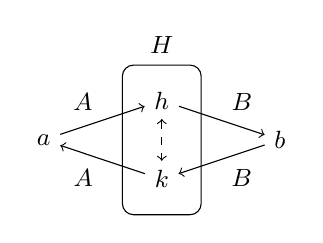
\begin{tikzpicture}[every node/.style={font=\small}]
\draw[rounded corners] (1.0,-.45) rectangle (2.0,1.45);
\node at (1.5,1.7) {$H$};
\node (fa) at (0,.5) {$a$}; \node (fh) at (1.5,1) {$h$};
\node (fb) at (3,.5) {$b$}; \node (fk) at (1.5,0) {$k$};
\draw[->] (fa)--node[above left] {$A$}(fh);
\draw[->] (fh)--node[above right] {$B$}(fb);
\draw[->] (fb)--node[below right] {$B$}(fk);
\draw[->] (fk)--node[below left] {$A$}(fa);
\draw[<->,dashed] (fh)--(fk);
\end{tikzpicture}
\caption{The cross-side cycle in a partial-order amalgam. Solid arrows are
the assumed weak comparisons, labeled by their original order.
Their composites force \(h\leq k\) and \(k\leq h\) inside the common
part \(H\), and then force \(a=h\), contrary to \(a\notin H\).
The relational data are those of \cite[Fig.~1, p.~386]{Fraisse1954}.}
\label{fig:p03-fraisse54-order-cycle}
\end{figure}

\begin{figure}[htbp]
\centering
\begin{tikzpicture}[scale=.9, every node/.style={font=\small}]
\node (a) at (0,1.6) {$a$}; \node (b) at (1.1,1.6) {$b$};
\node (c) at (2.2,1.6) {$c$}; \node (d) at (.55,0) {$d$};
\draw[->] (d)--(a); \draw[->] (d)--(b);
\node at (1.1,-.65) {$A$};
\node (aa) at (4,1.6) {$a$}; \node (bb) at (5.1,1.6) {$b$};
\node (cc) at (6.2,1.6) {$c$}; \node (e) at (5.65,0) {$e$};
\draw[->] (e)--(bb); \draw[->] (e)--(cc);
\node at (5.1,-.65) {$B$};
\node (aaa) at (8,1.6) {$a$}; \node (bbb) at (9.1,1.6) {$b$};
\node (ccc) at (10.2,1.6) {$c$};
\node (dd) at (8.7,-.2) {$d'$}; \node (ee) at (9.5,.5) {$e'$};
\draw[->] (dd)--(aaa); \draw[->] (dd)--(ee);
\draw[->] (ee)--(bbb); \draw[->] (ee)--(ccc);
\draw[->,dashed] (dd) to[bend right=20] (ccc);
\node at (9.1,-.85) {$d'<e'\text{ case}$};
\end{tikzpicture}
\caption{The ramified-order obstruction. Arrows show strict order;
reflexive pairs are implicit. The common base is the antichain
\(\{a,b,c\}\). An amalgam would have to compare the two predecessors of
\(b\), forcing a new comparison inside \(A\) or \(B\).
The dashed comparison in the displayed case contradicts the embedding of
\(A\); the reverse comparison gives the symmetric contradiction in \(B\).
Coincident images of \(d,e\) also force a forbidden comparison.
This redraws the relational data of \cite[Fig.~2, p.~387]{Fraisse1954}.}
\label{fig:p03-fraisse54-ramified}
\end{figure}

\begin{hbtheorem}{thm:p03-fraisse54-orders}{proved=annex:p3.fraisse54.orders}{Homogeneous orders and the countability boundary}
Initial and final segments here mean the strict segments below and above
a specified point; open intervals have two distinct endpoints in increasing
order.
A linear order is homogeneous exactly when its initial segments, final
segments and open intervals have types independent of their
chosen endpoints within each of these three families. For an order with
at least two elements, \(\mathcal H\) is equivalent to density and absence
of endpoints. Consequently the only nontrivial countable homogeneous order
is \((\mathbb Q,<)\).
There are uncountable homogeneous orders of different types, whereas
\(\mathbb R\setminus\{0\}\) satisfies \(\mathcal H\) and is not homogeneous.
\end{hbtheorem}

The source also asks about a merely universal countable ramified order.
Failure of amalgamation rules out a homogeneous representative of the full
age; it does not by itself rule out a countable universal host. These are
the separate questions distinguished in \cite[\S\S4.7, 9.5]{Fraisse1954}.

\section{The explicit countable-signature bridge}
\label{sec:p03-fraisse54-modern}

\begin{hbtheorem}{thm:p03-fraisse54-countable-language}{proved=annex:p3.fraisse54.countable-language}{Fra\"iss\'e limits in a countable relational signature}
Let \(\tau\) be a countable signature of relations of finite arity, with
no function or constant symbols. Let \(\mathcal K\) be a nonempty,
isomorphism-closed class of finite \(\tau\)-structures with countably many
isomorphism types and unbounded finite sizes. Then \(\mathcal K\) is the
age of a countably infinite ultrahomogeneous structure if and only if it
has the hereditary, joint-embedding and amalgamation properties.
The structure is unique up to isomorphism and is universal, by induced
embeddings, for countable structures whose age is contained in \(\mathcal K\).
\end{hbtheorem}

The proof uses an enumeration of finite structures and, at every stage,
the finitely many embeddings of finitely many enumerated structures into
the current stage. It does not assume that a countable signature has only
finitely many structures of a given finite size. In this theorem the age
itself must have countably many types. The original fixed-arity proof and
this enumeration are thus two explicit schedules for the same extension task.

\begin{hbtheorem}{thm:p03-fraisse54-categoricity-boundary}{proved=annex:p3.fraisse54.categoricity-boundary}{Finite signatures and a countable-signature counterexample}
In a finite relational signature with no function or constant symbols,
a countably infinite ultrahomogeneous
structure has quantifier elimination in its complete theory and is
\(\aleph_0\)-categorical. Empty conjunctions and disjunctions may be used
as logical truth and falsity in the quantifier-free language.
The corresponding claim for all countable relational signatures is false,
even for a Fra\"iss\'e class with countably many finite types and amalgamation.
\end{hbtheorem}

\section{The simple-graph interface}
\label{sec:p03-fraisse54-graph}

\begin{hbdefinition}{def:p03-fraisse54-graph-axioms}{Graph language and extension axioms}
A simple graph has one irreflexive symmetric binary relation \(E\).
For a tuple \(\bar w=(w_1,\ldots,w_m)\), let
\(\delta_m(\bar w)=\bigwedge_{1\leq i<j\leq m}w_i\ne w_j\).
For each pair \(r,s\geq0\), its extension axiom is
\[
 \begin{split}
 \forall w_1\cdots\forall w_{r+s}\bigl(&\delta_{r+s}(\bar w)\to
 \exists z\bigl(\delta_{r+s+1}(\bar w,z)\\
 &\land\bigwedge_{i=1}^{r}E(z,w_i)
 \land\bigwedge_{j=1}^{s}\neg E(z,w_{r+j})\bigr)\bigr).
 \end{split}
\]
An empty conjunction is truth, and an empty quantifier prefix is omitted.
The theory consists of these sentences together with
\(\forall x\neg E(x,x)\) and
\(\forall x\forall y(E(x,y)\leftrightarrow E(y,x))\).
\index{random graph!extension axioms}
\end{hbdefinition}

\begin{hbtheorem}{thm:p03-fraisse54-graph}{proved=annex:p3.fraisse54.graph}{Finite graph amalgams and the countable extension graph}
Finite simple graphs, with induced embeddings, form a Fra\"iss\'e class.
Its limit \(G\) is characterized among countable graphs by the property
\[
 \begin{gathered}
 U,V\subseteq G\text{ finite},\quad U\cap V=\varnothing
 \quad\Longrightarrow\\
 \exists z\in G\setminus(U\cup V)\;
   (\forall u\in U\;zEu)\ \land\ (\forall v\in V\;\neg zEv).
 \end{gathered}
\]
It is ultrahomogeneous, contains every countable simple graph as an induced
subgraph, and its extension axioms form a complete
\(\aleph_0\)-categorical first-order theory.
\end{hbtheorem}

The amalgam introduces
no edges between the new vertices on opposite sides. The theorem provides
the graph interface of \cref{thm:p03-random-graph}; its proof below is the
finite-amalgamation consequence, with no probability distribution assumed.

\section{First-order theories and the source's closing questions}
\label{sec:p03-fraisse54-logical-application}

\begin{hbtheorem}{thm:p03-fraisse54-logical-joint}{proved=annex:p3.fraisse54.logical-joint}{Common hosts for a complete first-order theory}
Let \(T\) be a satisfiable complete first-order theory in a relational
signature. Every set-indexed family of models of \(T\) embeds into one
model of \(T\). In fact the embeddings can be chosen elementary.
\end{hbtheorem}

This gives the joint-host conclusion for the source's arithmetic types
\cite[\S10.1]{Fraisse1954}, using first-order compactness and diagrams.
The stronger elementary formulation is justified by the supplied diagram
proof rather than attributed to the source's shorter formulation.

The four questions formulated in \cite[\S10.2]{Fraisse1954} concern:
\begin{enumerate}
\item whether agreement with a fixed age only on restrictions of size at
      most \(p\) still produces a class \(\Gamma_R\);
\item the number of local classes satisfying \(\mathcal D\), or
      \(\overline{\mathcal D}\);
\item whether testing extension to automorphisms only on restrictions of
      size at most the relation's arity implies full homogeneity;
\item replacing homogeneity by the condition that every finite set is
      contained in a finite larger set whose embeddings extend to
      automorphisms, and asking for a unique countable representative.
\end{enumerate}
The printed footnote already records a negative answer to the first question.
This paragraph identifies the historical questions; it makes no assertion
that the remaining questions are still open.

% N-a-002, original Rado1964 presentation, including the transfinite section.
\chapter{Rado's Universal Graphs and Functions}
\label{sec:p03-rado-1964}

Universality depends on the class of objects and on the maps allowed between
them. Rado's 1964 paper constructs universal countable graphs, uniform and
mixed complexes, and finite-colour functions by coding finite requirements
into integer digits. It also gives a nonuniversality theorem for locally finite
graphs and a separate transfinite function theorem under specified cardinal
arithmetic assumptions \cite[pp.~331--340]{Rado1964}.

The constructions retain these different domains. An induced graph embedding
preserves edges and nonedges; a colour-function embedding acts on the arguments
while leaving colours fixed. The transfinite section allows repeated earlier
arguments and a final maximum, unlike the strictly increasing finite tuples
used in the digit constructions. The ambient set theory is ZFC. Additional
GCH assumptions occur only where stated.

\section{Graphs, weak embeddings and binary digits}
\label{sec:p03-rado64-graphs}

\begin{hbdefinition}{def:p03-rado64-graph}{The source graph and embedding conventions}
A graph is a pair \(\Gamma=(A,B)\), where \(B\subseteq[A]^2\);
\([A]^r\) denotes the set of \(r\)-element subsets of \(A\).
Thus graphs here are simple and undirected. A weak embedding is an injection
\(\varphi:A\to A^*\) preserving edges. Write \(xE_\Gamma y\) for
\(\{x,y\}\in B\). An embedding additionally reflects
edges:
\[
 \{x,y\}\in B\quad\Longleftrightarrow\quad
       \{\varphi(x),\varphi(y)\}\in B^*\qquad(x\ne y).
\]
This is an induced embedding. A graph universal for a class belongs to the
class and admits the indicated embedding of every member of that class.
\end{hbdefinition}

The two vertices of an edgeless graph weakly embed into a single edge,
but do not embed as an induced subgraph. Replacing the embedding notion
changes the question \cite[1.1]{Rado1964}.

\begin{hbdefinition}{def:p03-rado64-digits}{Digits and the binary graph}
Write \(\mathbb N_0=\{0,1,2,\ldots\}\). For an integer base \(k\geq2\),
let \(d_k(t,j)\in\{0,\ldots,k-1\}\) be the \(j\)-th digit of \(t\in\mathbb N_0\):
\[
 t=\sum_{j\geq0}d_k(t,j)k^j.
\]
Only finitely many digits are nonzero. Rado's graph \(R\) has vertex set
\(\mathbb N_0\) and, for \(x<y\),
\[
 xE_Ry\quad\Longleftrightarrow\quad d_2(y,x)=1.
\]
Adjacency is extended symmetrically, with no loops.
\end{hbdefinition}

A nonzero \(x\)-th binary digit of \(y\) implies \(y\geq2^x>x\).
This explains the orientation implicit in the original definition using
the two-element set \(\{x,y\}\).

\begin{hbtheorem}{thm:p03-rado64-graph-universal}{proved=annex:p03.rado64.graph-universal}{Rado's Theorem 1: an explicit induced universal graph}
Every graph with at most countably many vertices embeds into \(R\).
For a graph labelled by \(\mathbb N_0\), an increasing embedding is obtained
recursively. At stage \(\xi\), choose a nonnegative integer \(\psi(\xi)\) larger than every
previous \(\varphi(x)\), \(x<\xi\), and put
\[
 \varphi(\xi)=2^{\psi(\xi)}
       +\sum_{\substack{x<\xi\\xE_\Gamma\xi}}2^{\varphi(x)}.
\]
The unused high digit makes the map increasing without changing its required
adjacency digits.
\end{hbtheorem}

The recursion is effective relative to the input graph's adjacency information;
arbitrary countable graphs need not have computable adjacency. Universality
does not require surjectivity or imply uniqueness among all universal graphs.

\section{The extension property and the Fra\"iss\'e interface}
\label{sec:p03-rado64-extension}

\begin{hbtheorem}{thm:p03-rado64-extension}{proved=annex:p03.rado64.extension}{Finite adjacency patterns and the countable extension graph}
For disjoint finite \(U,V\subseteq R\), infinitely many vertices outside
\(U\cup V\) are adjacent to all of \(U\) and to none of \(V\).
Any two countable graphs with this property are isomorphic, and every
isomorphism between finite induced subgraphs of one extends to an automorphism.

In particular \(R\) is isomorphic to the graph in
\cref{thm:p03-fraisse54-graph}. Its extension axioms form the same complete
\(\aleph_0\)-categorical theory. These are the explicit modern graph
consequences, not additional assertions attributed to Rado's Theorem 1.
\end{hbtheorem}

\begin{hbtheorem}{thm:p03-rado64-amalgams}{proved=annex:p03.rado64.amalgams}{A graph amalgam and an amalgamation failure}
Finite simple graphs have the hereditary, joint-embedding and amalgamation
properties for induced embeddings. Their free amalgam identifies the common
induced graph and adds no edges between the two new sides.

Finite forests fail amalgamation for induced embeddings. Take a common graph
of two nonadjacent vertices \(a,b\), one extension \(a-x-b\) and another
\(a-y-z-b\), each an induced path. These have no common forest amalgam.
\end{hbtheorem}

A structural embedding is not by definition a partial elementary map.
The first-order graph conclusions use the separately supplied extension-axiom
argument. The deterministic binary graph is not a distribution on finite graphs.

\section{Why locally finite graphs have no universal member}
\label{sec:p03-rado64-locally-finite}

\begin{hbdefinition}{def:p03-rado64-local}{Local finiteness and finite-step reachability}
A graph is locally finite if each vertex has finitely many neighbours.
For \(m\geq1\), let \(k(\Gamma,x,m)\) count vertices reachable from \(x\)
by a walk of exactly \(m\) edges; vertices in a walk may repeat.
This count is finite in a locally finite graph.

Rado calls an acyclic graph a tree. The specific tree below is also connected,
so the distinction between tree and forest does not affect the construction.
\end{hbdefinition}

\begin{hbtheorem}{thm:p03-rado64-no-local-universal}{proved=annex:p03.rado64.no-local-universal}{Theorem 2, communicated by N. G. de Bruijn}
The class of countably infinite locally finite graphs has no weakly universal
member. For every countably infinite locally finite graph \(H\), there is
a countably infinite locally finite tree that does not weakly embed into \(H\).
\end{hbtheorem}

The candidate host must itself be locally finite. Rado's binary graph has
infinite vertex degrees, so there is no contradiction with Theorem 1.

\section{The binomial code for fixed-size sets}
\label{sec:p03-rado64-binomial}

\begin{hbdefinition}{def:p03-rado64-combinadic}{Rado's increasing-tuple code}
For an integer \(\ell\geq1\) and \(0\leq x_0<\cdots<x_{\ell-1}\), put
\[
 \tau(x_0,\ldots,x_{\ell-1})
       =\sum_{i=0}^{\ell-1}\binom{x_i}{i+1}.
\]
Use \(\binom ab=0\) for integers \(0\leq a<b\).
For the empty tuple put \(\tau(\varnothing)=0\).
Colexicographic order compares tuples at their largest coordinate of
disagreement.
\end{hbdefinition}

\begin{hbtheorem}{thm:p03-rado64-combinadic}{proved=annex:p03.rado64.combinadic}{The lemma of Section 2.2}
For each fixed \(\ell\geq1\), \(\tau\) is an order-preserving bijection from
increasing \(\ell\)-tuples of nonnegative integers in colexicographic order
onto \(\mathbb N_0\). Distinct \(\ell\)-element sets receive distinct digit
positions.
\end{hbtheorem}

This is the original fixed-dimension code. Mixed dimensions use a different
finite-subset code.

\section{Uniform and mixed complexes}
\label{sec:p03-rado64-complexes}

\begin{hbdefinition}{def:p03-rado64-complex}{The source's complex conventions}
An \(\ell\)-dimensional complex is \(C=(A,B)\) with
\(B\subseteq[A]^{\ell+1}\). An embedding is an injection preserving and reflecting
membership of every \((\ell+1)\)-element subset.
A mixed complex has
\[
 B\subseteq[A]^{<\omega}\setminus\{\varnothing\},
\]
allowing unbounded finite simplex sizes. No downward-closure condition is
imposed. The term is used in Rado's specified sense, not replaced by another
convention for abstract simplicial complexes.
\end{hbdefinition}

\begin{hbtheorem}{thm:p03-rado64-uniform-complex}{proved=annex:p03.rado64.uniform-complex}{Rado's Theorem 3}
For \(\ell\geq1\), define \(C_\ell^*\) on \(\mathbb N_0\) by
\[
 \{x_0<\cdots<x_\ell\}\in B_\ell^*
 \quad\Longleftrightarrow\quad
 d_2(x_\ell,\tau(x_0,\ldots,x_{\ell-1}))=1.
\]
It is universal for at most countable complexes of this dimension.
For \(\ell=0\), the analogous universal complex takes the odd vertices
as its singleton simplices.
\end{hbtheorem}

\begin{hbdefinition}{def:p03-rado64-mixed-code}{The source's mixed-length code}
For an increasing tuple \(0\leq x_0<\cdots<x_{\ell-1}\), with
\(\ell\geq0\), put
\[
 \rho(x_0,\ldots,x_{\ell-1})=\sum_{i<\ell}2^{x_i}.
\]
The empty tuple has code zero. Identifying a finite subset with its unique
increasing enumeration, binary expansion makes \(\rho\) a bijection from
all finite subsets of \(\mathbb N_0\) onto \(\mathbb N_0\).
The code \(\tau\) is injective only after the tuple length has been fixed;
\(\rho\) distinguishes lengths as well as the entries.
\end{hbdefinition}

\begin{hbtheorem}{thm:p03-rado64-mixed-complex}{proved=annex:p03.rado64.mixed-complex}{Rado's Theorem 4}
The mixed complex on \(\mathbb N_0\) given by
\[
 \{x_0<\cdots<x_\ell\}\in B_{\rm mix}^*
 \quad\Longleftrightarrow\quad
 d_2(x_\ell,\rho(x_0,\ldots,x_{\ell-1}))=1,\qquad\ell\geq0,
\]
is universal for at most countable mixed complexes.
The singleton case uses digit zero of its vertex.
\end{hbtheorem}

The source excludes the empty simplex. If membership of the empty set were
an additional freely varying truth value, a single host could not represent
both values: every embedding maps the empty set to itself.

\section{Universal finite-colour functions}
\label{sec:p03-rado64-finite-functions}

\begin{hbdefinition}{def:p03-rado64-colour-functions}{The classes \(K_{k\ell}\) and \(K_k\)}
For integers \(k\geq2\), \(\ell\geq0\), \(K_{k\ell}\) consists of functions
on increasing \((\ell+1)\)-tuples of \(\mathbb N_0\) with values in
\(\{0,\ldots,k-1\}\). The class \(K_k\) uses all nonempty finite increasing
tuples with the same colour set.
A universal member \(f^*\) represents every \(f\) through one injection
\(\varphi:\mathbb N_0\to\mathbb N_0\), preserving the argument domain, such that
\[
 f(x_0,\ldots,x_\ell)=
       f^*(\varphi(x_0),\ldots,\varphi(x_\ell)).
\]
The constructed maps are increasing. Arguments are mapped, while colours
remain fixed.
\end{hbdefinition}

\begin{hbtheorem}{thm:p03-rado64-finite-colours}{proved=annex:p03.rado64.finite-colours}{Rado's Theorem 5}
For \(\ell\geq1\), a universal member of \(K_{k\ell}\) is
\[
 f_{k\ell}^*(x_0,\ldots,x_\ell)
       =d_k(x_\ell,\tau(x_0,\ldots,x_{\ell-1})).
\]
For \(\ell=0\), use \(f_{k0}^*(x)=d_k(x,0)\).
This unary clause is included as a separately proved boundary extension;
the printed Theorem 5(a) assumes \(\ell\geq1\).
A universal member of \(K_k\) is
\[
 f_k^*(x_0,\ldots,x_\ell)=
       d_k(x_\ell,\rho(x_0,\ldots,x_{\ell-1})).
\]
All representing injections can be chosen increasing.
\end{hbtheorem}

The binary complexes are the \(k=2\) cases. Rado also interprets colours as
coefficients modulo \(k\); a chosen increasing vertex order then determines
the canonical order for oriented simplices, preserved by the embeddings.
No face-closure or chain-complex axiom is inferred.

These classes are not the class of all algebraic operations on all ordered
tuples. Repetitions, arbitrary order and infinitely many colours require
their own argument domains and proofs.

\section{The transfinite domain and index notation}
\label{sec:p03-rado64-transfinite-data}

\begin{hbconvention}{def:p03-rado64-transfinite-indices}{Initial ordinals and Rado's cofinality indices}
Write \(\omega_n\) for the initial ordinal of cardinality \(\aleph_n\).
Rado's index-valued notation \(\mathrm{cf}(n)\) is the ordinal satisfying
\[
 \operatorname{cf}(\aleph_n)=\aleph_{\mathrm{cf}(n)}.
\]
The left-hand \(\operatorname{cf}\) is ordinary cardinal cofinality;
\(\mathrm{cf}(n)\) on the right is its aleph index, not ordinary
cofinality of the ordinal \(n\). The source also uses \(n-1=r\) if
\(n=r+1\), and \(n-1=n\) if \(n\) has no immediate predecessor.
In this convention the displayed \(n-1\) is a predecessor notation,
including at zero and limit ordinals, rather than ordinal subtraction.
The ordinary cardinal and cofinality conventions are those of
\cref{entry:p06-source-30,def:p06-cofinality-regular-singular}.
\end{hbconvention}

\begin{hbdefinition}{def:p03-rado64-transfinite-domain}{The class \(F(l,m,S)\)}
Let \(l,m\) be ordinals and \(S\ne\varnothing\).
For every \(\lambda<l\), the argument sequences
\(\bar x=(x_i)_{i\leq\lambda}\) have length \(\lambda+1\) and satisfy
\[
 x_i\leq x_\lambda<m\quad(i<\lambda).
\]
Earlier coordinates need not increase or be distinct, and may equal the
final coordinate. \(F(l,m,S)\) is the set of functions on the disjoint union
of these domains, with values in \(S\).
Its universal \(f^*\) represents every \(f\) by one injection \(\varphi:m\to m\)
that preserves the domain and satisfies
\[
 f((x_i)_{i\leq\lambda})=f^*((\varphi(x_i))_{i\leq\lambda}).
\]
For \(l=0\) there are no argument tuples. The constructions below use
increasing injections on the stated initial-ordinal domains; no transfer
to arbitrary ordinal order types of the same cardinality is assumed.
\end{hbdefinition}

\begin{hbtheorem}{thm:p03-rado64-order-type-boundary}{proved=annex:p03.rado64.order-type-boundary}{The argument order type cannot be replaced by its cardinality}
The class \(F(2,\omega+1,\{0,1\})\) has no universal member,
although \(F(2,\omega,\{0,1\})\) has one by the countable case
of Theorem 6 below. The two argument domains have the same cardinality.
\end{hbtheorem}

\begin{hbtheorem}{thm:p03-rado64-restriction}{proved=annex:p03.rado64.restriction}{Reducing arities and the colour set}
If \(F(l,m,S)\) has a universal member, then so does
\(F(l_0,m,S_0)\) for \(l_0\leq l\) and
\(\varnothing\ne S_0\subseteq S\).
The reduction uses restriction and a colour-set retraction; the original
universal function need not already take its values in \(S_0\).
\end{hbtheorem}

\begin{hbdefinition}{def:p03-rado64-marked-template}{A template for a new maximum}
For a bound \(\eta\) in an ordered domain put
\(D_\eta=\{x:x<\eta\}\sqcup\{*\}\), with a new marker \(*\).
An \(l\)-template is a function
\[
 h:\bigsqcup_{\lambda<l}D_\eta^\lambda\longrightarrow S.
\]
Suppose each vertex \(z\) has been assigned one pair \((\eta_z,h_z)\).
For a tuple \((y_i)_{i\leq\lambda}\) ending at \(z=y_\lambda\), define
\[
 f^*((y_i)_{i\leq\lambda})=h_z((u_i)_{i<\lambda}),\qquad
 u_i=\begin{cases}y_i,&y_i<\eta_z,\\ *,&y_i\geq\eta_z.\end{cases}
\]
The tagged disjoint union retains the prefix length, even for an empty
prefix. This supplies a total function on the stated domain once the
assignments are fixed.
In the embedding construction, \(*\) denotes arguments equal to the newly
embedded maximum; all earlier images have already been placed below \(\eta\).
\end{hbdefinition}

\section{The three transfinite regimes}
\label{sec:p03-rado64-transfinite-theorem}

\begin{hbtheorem}{thm:p03-rado64-transfinite}{proved=annex:p03.rado64.transfinite}{Rado's Theorem 6 with the non-strict final-maximum domain}
Let \(l,n\) be ordinals and assume
\[
 2^{\aleph_\nu}=\aleph_{\nu+1}\qquad(\nu<n).
\]
The class \(F(l,\omega_n,S)\) has a universal member in each case:
\begin{enumerate}
\item \(n=n-1=\mathrm{cf}(n)\), \(l<\omega_n\), \(1\leq|S|\leq\aleph_n\);
\item \(n=r+1\), \(l<\omega_{\mathrm{cf}(r)}\), \(1\leq|S|\leq\aleph_n\);
\item \(n>\mathrm{cf}(n)\), \(l<\omega_n\), \(1\leq|S|<\aleph_n\).
\end{enumerate}
Its representing injections may be chosen increasing.
\end{hbtheorem}

In the first case the target is regular and either countable or a limit
cardinal. In the second it is a successor, with arity bound below its
predecessor's cofinality. In the third it is singular and the number of
colours has a strict upper bound. No GCH assumption entered the integer-digit
constructions.

The proof makes repeated occurrences of the final maximum explicit using
the marker in \cref{def:p03-rado64-marked-template}. Thus its requirements
are specified before the new image is chosen. Cardinal estimates and
regular/singular scheduling then establish the full stated non-strict domain.

Rado closes by asking how essential the transfinite argument restrictions
and successor-length tuples are, and for nontrivial nonuniversality cases.
These are the paper's historical questions, not assertions of present open
status or permission to remove the theorem's restrictions.

\begin{hbtheorem}{thm:p03-rado64-arity-obstruction}{proved=annex:p03.rado64.arity-obstruction}{Why all finite repeated-argument arities change the problem}
The class \(F(\omega,\omega,\{0,1\})\) has no universal member.
This is an additional explicit boundary example: it does not contradict
Theorem 5, whose arguments are strictly increasing and hence distinct.
\end{hbtheorem}

\section{Choosing the relevant universal object}
\label{sec:p03-rado64-reference}

The binary graph addresses induced embeddings of countable simple graphs.
The locally finite result changes the host class and fails even for weak
embeddings. Uniform complexes fix subset size; mixed complexes allow all
finite nonempty sizes. Finite-colour functions preserve colour values, while
the transfinite theorem uses a different sequence domain and additional
cardinal hypotheses.

For graphs, specify reflection of nonedges, the host class and countability.
For functions, specify arity, repetition, order, colours and the representation
map. The common word \emph{universal} cannot replace these distinctions.

\chapter*{Further Reading for Part III}
\addcontentsline{toc}{chapter}{Further Reading for Part III}
\chaptermark{Further Reading for Part III}
\label{sec:p03-further-reading}

These sources extend the exact inherited chapters and the separately authored
surveys without changing any theorem's proof status.

\begin{description}
  \item[Maps, elementary substructures, and diagrams.]
    See \textcite{Marker2002,Hodges1993}.
  \item[Types, ultrafilters, ultraproducts, and saturation.]
    See \textcite{ChangKeisler1990,Marker2002}; the original ultraproduct source
    is \textcite{Los1955Ultraproducts}.
  \item[Quantifier elimination, categoricity, and games.]
    See \textcite{Hodges1993,Marker2002}.
  \item[Classification and countable models.]
    See \textcite{Fraisse1954,Rado1964,Marker2002,Hodges1993,
    BaldwinLachlan1971,Shelah1971NonIsomorphicModels,TentZiegler2012}.
  \item[Finite model theory.]
    See \textcite{EbbinghausFlum1995,Libkin2004}.
  \item[Preservation and abstract model theory.]
    See \textcite{RobinsonJointConsistency1956,Beth1953,Craig1957,
    ChangKeisler1990,Lindstrom1969,BarwiseFeferman1985,Keisler1970,
    Vaananen2007}.
\end{description}

